%% LyX 1.1 created this file.  For more info, see http://www.lyx.org/.
%% Do not edit unless you really know what you are doing.
\documentclass[english,twoside]{article}
\usepackage[T1]{fontenc}
\usepackage{geometry}
\geometry{verbose,letterpaper}
\usepackage{fancyhdr}
\pagestyle{fancy}
\usepackage{babel}
\setlength\parskip{\medskipamount}
\setlength\parindent{0pt}
\usepackage{graphicx}
\usepackage{wrapfig}
\usepackage{comment}
\usepackage{amsmath} %uncommented by MT 5/2015, used in "E near charged rod"
\setlength\topmargin{0.2in}
\addtolength{\hoffset}{-1.0cm}
\addtolength{\textwidth}{2.0cm}
\addtolength{\voffset}{-1.5cm} %This line is apparently needed on MikTex XeLatex.  Comment out if your pages appear shifted too high.
\addtolength{\textheight}{3.5cm}
% define a strut for extra vertical space in tables.
\newcommand{\hi}{\rule[-2mm]{0mm}{6mm}}

%The \includonly line below is a great way to save time so you don't always have to compile the WHOLE latex document, if for instance you've only made changes to a single lab.  If you want to compile more than two labs, the syntax is \includeonly{lab1,lab2,lab3} with no spaces after the commas.
%The master.pdf produced will have only the title page, TOC, and that single lab, though the other lab names will appear in the TOC.
%\includeonly{calorimetry/calorimetry}

\makeatletter

%%%%%%%%%%%%%%%%%%%%%%%%%%%%%% LyX specific LaTeX commands.
\providecommand{\LyX}{L\kern-.1667em\lower.25em\hbox{Y}\kern-.125emX\@}
\newenvironment{LyXParagraphIndent}[1]%
{
  \begin{list}{}{%
    \setlength\topsep{0pt}%
    \addtolength{\leftmargin}{#1}
    \setlength\parsep{0pt plus 1pt}%
  }
  \item[]
}
{\end{list}}
%% Special footnote code from the package 'stblftnt.sty'
%% Author: Robin Fairbairns -- Last revised Dec 13 1996
\let\SF@@footnote\footnote
\def\footnote{\ifx\protect\@typeset@protect
    \expandafter\SF@@footnote
  \else
    \expandafter\SF@gobble@opt
  \fi
}
\expandafter\def\csname SF@gobble@opt \endcsname{\@ifnextchar[%]
  \SF@gobble@twobracket
  \@gobble
}
\edef\SF@gobble@opt{\noexpand\protect
  \expandafter\noexpand\csname SF@gobble@opt \endcsname}
\def\SF@gobble@twobracket[#1]#2{}

\makeatother


%I make use of some latex features to manage the section numbers. To use those you have to insert the following lines into the latex preamble (before the %"\begin{document}" command).

% two new commands to do labelling. - gpg 12/4/13
\newcommand{\customlabel}[2]{%
\protected@write \@auxout {}{\string \newlabel {#1}{{#2}{}}}}

\newcommand{\actlabel}[1]{%
\protected@write \@auxout {}{\string \newlabel {#1}{{\arabic{activity}}{}}}}

\newcounter{activity}

\begin{document}

\title{Investigative Physics\\
Module 2: Activity Units for Physics 132}


\author{Emory F. Bunn,$^1$ Mirela Fetea,$^4$ Gerard P. Gilfoyle,$^1$ Henry Nebel,$^1$ \\Jack Singal,$^1$ Matthew Trawick,$^1$ Philip D. Rubin,$^2$ and Michael F. Vineyard$^3$\\[4pt]
$^1$Department of Physics, University of Richmond, VA \\[4pt]
$^2$Department of Physics, George Mason University, Fairfax, VA \\[4pt]
$^3$Department of Physics, Union College, Schenectady, NY \\[4pt]
$^4$Germanna Community College, Fredericksburg, VA 22408}


\maketitle
\begin{abstract}
The exercises in this manual have been developed to support an investigative
physics course that emphasizes active learning. Some of these units
have been taken from the Workshop Physics project at Dickinson College
and the Tools for Scientific Thinking project at Tufts University
and modified for use at the University of Richmond. Others have been
developed locally. 

The units are made up of activities designed to guide your investigations
in the laboratory. The written work will consist primarily of documenting
your class activities by filling in the entries in the spaces provided
in the units. The entries consist of observations, derivations, calculations,
and answers to questions. Although you may use the same data and graphs
as your partner(s) and discuss concepts with your classmates, all
entries should reflect your own understanding of the concepts and
the meaning of the data and graphs you are presenting. Thus, each
entry should be written in your own words. Indeed, it is very important
to your success in this course that your entries reflect a sound understanding
of the phenomena you are observing and analyzing. 

We wish to acknowledge the support we have received for this project
from the University of Richmond and the Instrumentation and Laboratory
Improvement program of the National Science Foundation. Also, we would
like to thank our laboratory directors for their invaluable technical
assistance.
\end{abstract}

\begin{center}

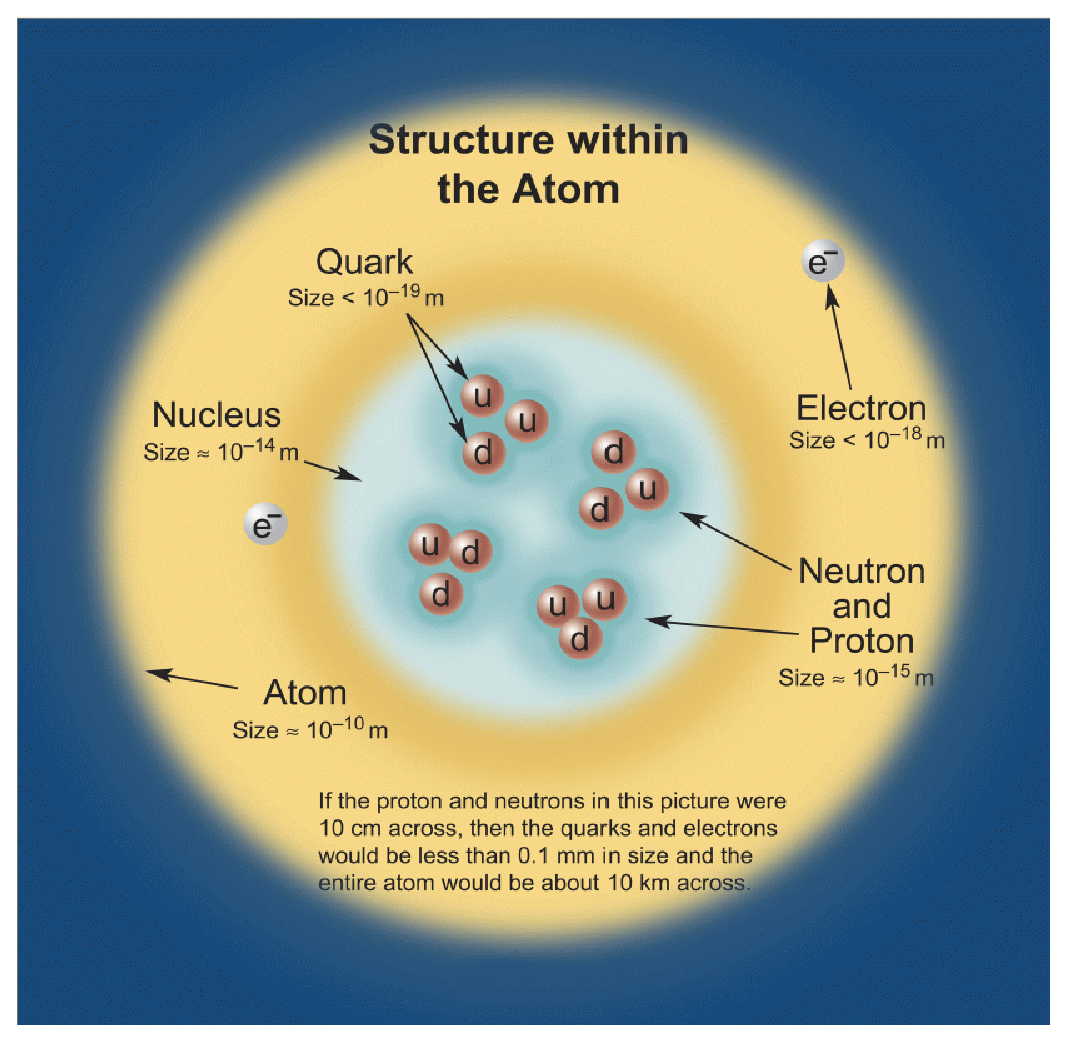
\includegraphics[width=3.2in]{AtomicStructure.ps}

\end{center}

\thispagestyle{empty}

\newpage

\
\setcounter{page}{1}

\vfill

Cover art: The atom consists of smaller electrons and a nucleus consisting of protons and neutrons. The protons and neutrons, in turn, are formed from objects called quarks and gluons. Courtesy, the American Institute of Physics.

\pagebreak

\tableofcontents{}


\section{Heat, Temperature, and Internal Energy}

\makelabheader %(Space for student name, etc., defined in master.tex)

\textbf{Objective}

To investigate the relationship between heat and temperature.

\textbf{Apparatus}

\begin{itemize}
\item Glass beaker 
\item Glass stirring rod
\item Hot plate
\item Ice
\item Pasco 550 interface
\item Temperature probe
\item Clamp and stand
\item Capstone software (\filename{Heat\_Temp\_Internal\_Energy.cap} experiment file)
\end{itemize}
\textbf{Temperature of a Substance as a Function of Heat Transfer}

As part of our quest to understand heat energy transfer, temperature,
and internal energy of a substance, let's consider the temperature
change as ice is changed to water and then to steam.

\textbf{Activity 1: Predicting T \textit{vs.}~t for Water} 

Suppose you were to add heat at a constant rate to a container of
ice water at 0\( ^{\circ } \)C until the water begins to boil. Sketch
the predicted shape of the heating curve on the graph below using
a dashed line. Mark the points at which the ice has melted and the
water begins to boil.

\vspace{0.3cm}
{\centering 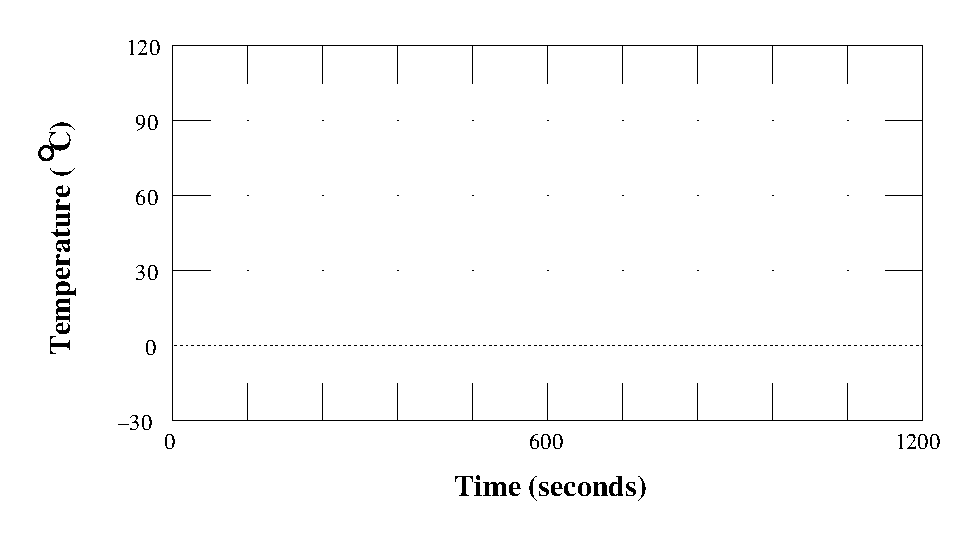
\includegraphics{heat_temp_int_energy/heat_temp_int_energy_fig_1.eps} \par}
\vspace{0.3cm}

\newpage

\textbf{Activity 2: Measuring T \textit{vs.}~t for Water} 

(a) To test your prediction: 

\begin{enumerate}
\item Fill the glass beaker one third full of ice and set it on top of the hot plate.
\item Suspend the temperature probe so that the end is submerged in the ice but not touching the side or bottom of the beaker. You will need to use the clamp and stand to do this. BE SURE THE WIRE FROM THE TEMPERATURE PROBE IS NOT TOUCHING THE HOT PLATE OR GLASS BEAKER. Also, be sure the temperature probe is attached to port ``A'' of the Pasco interface. Let set for 60 seconds so temperature probe can come to equilibrium with the ice.
\item Open the \filename{Heat\_Temp\_Internal\_Energy.cap} experiment file in the
\filename{\coursefolder} folder.
\item Turn on the hot plate to about 6 and click the
\button{Record} button on the monitor to begin recording data. The temperature of the water will be recorded on the graph shown on the monitor. Stir often to keep ice against the temperature probe.
\item When ice begins to turn to water, stir at about 1 minute intervals. When all ice is melted, there is no need to stir any further.
\item After the water begins to boil, keep hot plate on for a minute or two as temperature flattens at 100 degrees.
\item Stop data collection using the \button{Stop} button and turn off hot plate.
\item Sketch the shape of the measured heating curve on the above graph
using a solid line. Ignore small variations due to noise and uneven
heating. Mark the points at which the ice has melted and the water
begins to boil.
\item Print your graph and attach to this unit.
\end{enumerate}
(b) Does your prediction agree with the measured heating curve? If
not, what are the differences?
\vspace{15mm}

(c) What is the relationship between the temperature and the added
heat while the ice is melting?
\vspace{15mm}

(d) What is the relationship between the temperature and the added
heat after the ice has melted, but before the water begins to boil?
\vspace{15mm}

(e) What is the relationship between the temperature and the added
heat while the water is boiling?
\vspace{15mm}

(f) If there are regions of the heating curve in which the temperature
is not changing, what do you think is happening to the added heat
in these regions?\vspace{20mm}



\section{Calorimetry}

\makelabheader %(Space for student name, etc., defined in master.tex)

\bigskip
\textbf{Objectives}
\begin{itemize}[nosep]%[itemsep=1pt]%
\item To learn to use a method for measuring heat called calorimetry.
\item To use calorimetry to determine the specific heat of aluminum and
the heat of fusion of ice.
\end{itemize}

\bigskip
\textbf{Apparatus}

\begin{center}
\begin{tabular}{lll}
\textbullet \  Hypsometer    & \hspace{0.25in}\textbullet \  Calorimeter         & \hspace{0.25in}\textbullet \  Safety goggles \\
\textbullet \  Hot plate     & \hspace{0.25in}\textbullet \  Temperature probe   & \hspace{0.25in}\textbullet \  Compact scale (for measuring masses) \\
\textbullet \  Metal pellets & \hspace{0.25in}\textbullet \  Glass stirring rod  & \hspace{0.25in}\textbullet \  \textit{Capstone} software (\filename{Calorimetry.cap}) \\
\textbullet \  Plastic beaker& \hspace{0.25in}\textbullet \  Pasco 550 Interface & \hspace{0.25in} \\
\textbullet \  Ice           & \hspace{0.25in}\textbullet \  Clamp and stand     & \hspace{0.25in} \\
\end{tabular}
% \begin{tabular}{llll}
% \textbullet \  Hypsometer    &\textbullet \  Ice                &\textbullet \  Pasco 550 Interface                            & \textbullet \ Safety goggles   \\[2pt]
% \textbullet \  Hot plate     &\textbullet \  Calorimeter        &\textbullet \  Clamp and stand                                &  \\[2pt]
% \textbullet \  Metal pellets &\textbullet \  Temperature probe  &\textbullet \  \textit{Capstone} (\filename{Calorimetry.cap}) &  \\[2pt]
% \textbullet \  Plastic beaker&\textbullet \  Glass stirring rod &\textbullet \  Compact scale (for measuring masses)           &  \\
% \end{tabular}
\end{center}

\begin{center}
\begin{tabular}{ccc}
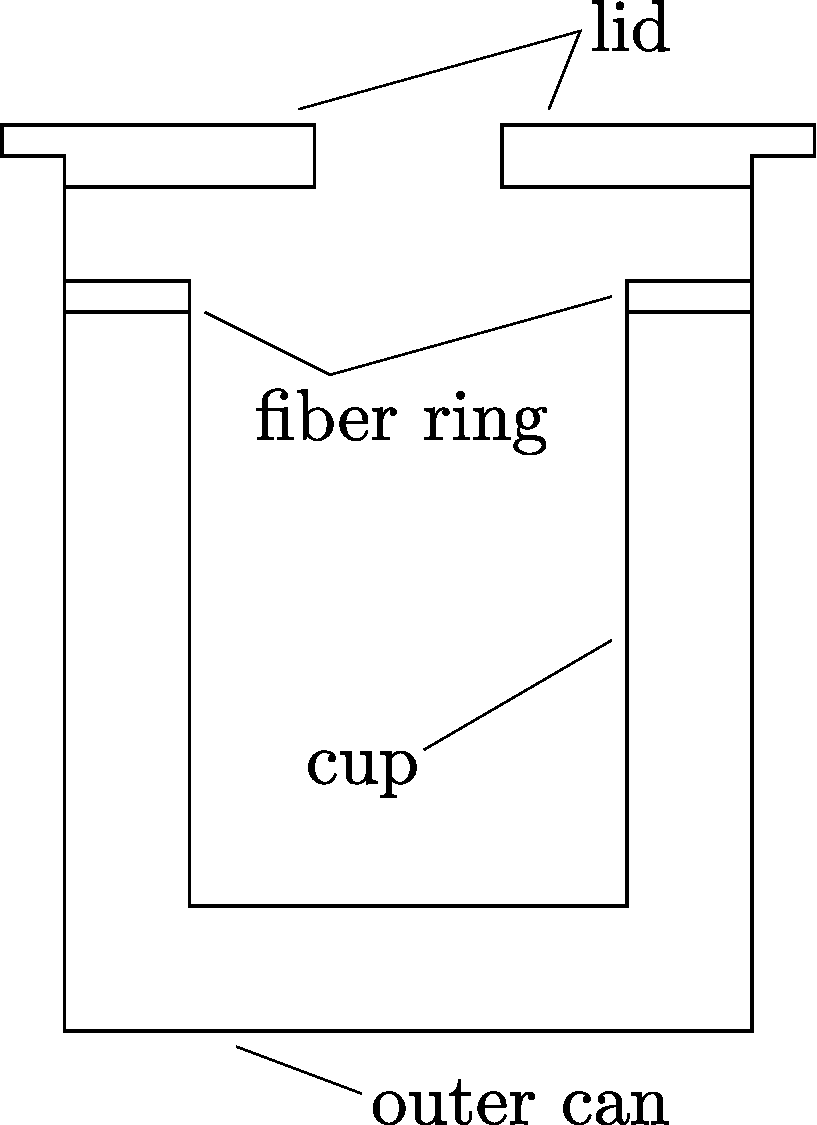
\includegraphics[height=3.0in]{calorimetry/calorimeter1.pdf} & \hspace{0.6in} & 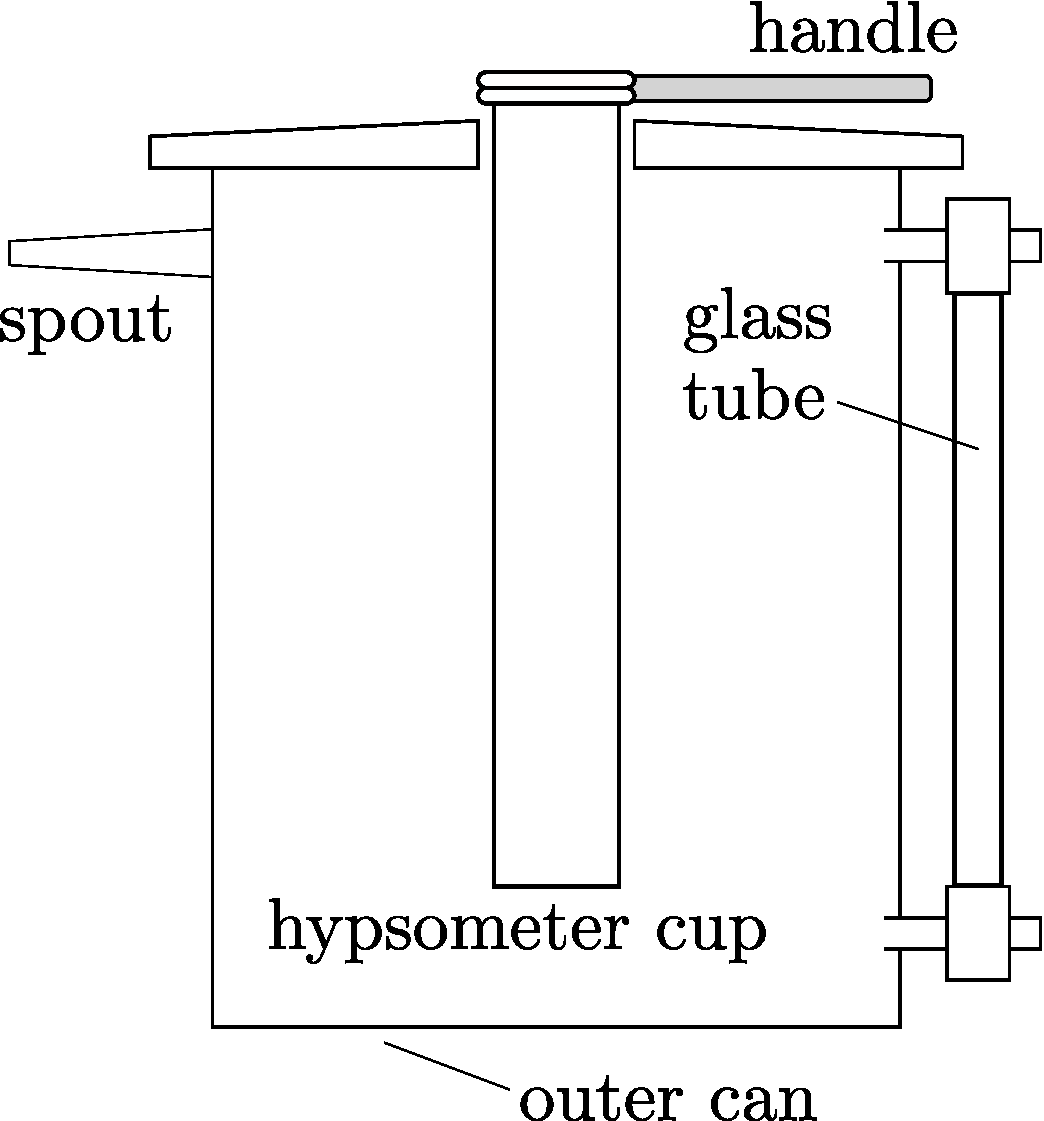
\includegraphics[height=3.0in]{calorimetry/hypsometer1.pdf} \\[5pt]
\LARGE Calorimeter                                           &                & \LARGE Hypsometer  \\
\end{tabular}
\end{center}

\bigskip
\textbf{Introduction} 

Calorimetry is a method for measuring heat. As applied in this experiment,
the method involves the mixing together of substances initially at
two different temperatures. The substances at the higher temperature
lose heat and the substances at the lower temperature gain heat until
thermal equilibrium is reached.

%\textbf{Experimental Equipment} 

A calorimeter, shown in the left-hand side of the figure, is used in this experiment
to minimize the exchange of heat between the system and the surroundings.
The inner calorimeter cup is thermally insulated from the surroundings
by suspending it on a ring of material with low heat conductivity
and surrounding it with a layer of air. Also the cup is shiny to minimize
radiation loss. Hence, if the mixture of substances is placed inside
the calorimeter cup, the heat lost to or gained from the surroundings
can be ignored, and the above relationship can be used. The only part
of the calorimeter which is involved in the calculation is the inner
calorimeter cup which contains water and in which an exchange of heat
between the hot and cold bodies takes place. The cup will undergo
the same temperature change as the contained water. Of course, an
instrument will have to be introduced to measure the temperature of
the system, but the heat gained or lost by the instrument is small
and can be ignored.

\pagebreak[3]

\textbf{Activity 1: Statement of Conservation of Energy}

If no heat is transferred to the surroundings, what is the relationship
between the heat lost by the substances initially at high temperature
and the heat gained by the substances initially at low temperature?
Note: This is simply a statement of conservation of energy.
\answerspace{15mm}

\textbf{Activity 2: Specific Heat of a Metal}

(a) Fill the hypsometer (boiler, shown in the right-hand side of the figure) 
at least half full of water and start heating the water. 
To avoid evaporating all the water (and possibly starting a fire) monitor 
the glass tube on the hypsometer for the water level.
If the water disappears turn the power off.
Ask your instructor which metal pellets to use for this activity.
Record the type of metal.
\answerspace{10mm}

(b) Determine and record the mass of the hypsometer cup, $m_h$.
Then fill it about half full with dry metal pellets. Determine
and record the mass of the cup and pellets, $m_{hp}$, and calculate
the mass of the pellets, $m_p$. Record the measurements here:
\answerspace{10mm}

(c) Fill the plastic beaker with ice water. Open the file \filename{Calorimetry.cap}
in the \filename{\coursefolder} folder and start
collecting data. To make sure the temperature probe is working 
properly place it in the ice water and
check that it is reading approximately 0~$^{\circ }$C. If not,
then consult your instructor.

(d) Place the hypsometer cup in the top of the hypsometer and put the temperature probe into the middle of the pellets.  To do this, remove the pellets from the cup, place the temperature probe in the proper position (using the clamp and stand), then return the pellets to the cup.

(e) Determine and record the mass of the calorimeter cup, $m_c$.
Fill this cup about half full of cold tap water. Determine and record
the mass of the cup and water, $m_{cw}$, and calculate the mass
of the water, $m_w$. Then place the calorimeter cup in the outer
can and put the lid on.
\vspace{15mm}

(f) When the temperature of the pellets becomes constant, at or near
100~$^{\circ }$C, record the temperature of the pellets as $T_{p}$.
Remove the probe from the pellets and put it in the cold water in the calorimeter cup. When the temperature of the water levels off, record it as $T_{w}$.
\vspace{15mm}

\pagebreak[3]
(g) Now, quickly but carefully, pour the pellets into the water in
the calorimeter cup. Stir the water occasionally with the glass stirring rod and
monitor the temperature of the mixture. When the temperature levels off, record
this value as $T$. Click the {\bf Stop} button on the monitor, print your graph of temperature as a function of time and include it in this unit.
\answerspace{20mm}
%\vspace{15mm}

(h) Write the complete heat equation and solve for the unknown specific
heat of the metal pellets.
The specific heat of the calorimeter cup is 900~J/kg$\cdot^{\circ}$C.
\answerspace{1.8in}

(i) Look up the accepted value for the specific heat of your metal and
calculate the percent difference between this value and the one you
determined above. Do the two values agree within experimental uncertainties?
Comment on possible sources of error.
\answerspace{20mm}

\textbf{Activity 3: Specific Heat of Another Metal}

(a) Repeat steps 2(a)--2(i) with pellets of a different metal.
Record the type of metal, the mass of the pellets, the temperature of the
pellets just before you pour them in the cold water, and the temperature of the
combined pellets, water, and cup.
\answerspace{15mm}

(b) Use the equation you derived above for the unknown specific
heat of the new metal. 
The specific heat of the calorimeter cup is 900~J/kg$\cdot^{\circ}$C.

\answerspace{2.5cm}

(c) Look up the accepted value for the specific heat of your new metal and
calculate the percent difference between this value and the one you
determined above. 
\answerspace{25mm}

\pagebreak[3]
\textbf{Activity 4: Average and Standard Deviation}

Consult the other lab groups in class and record their values of the specific
heats below.
Calculate the average and standard deviation for each metal.
%Can you spot any trends in your data?
\answerspace{1.2in}

%(e) The specific heats you measured above were in units of J/kg-\( ^{\circ } \)C. It is more illuminating  to express the the specific heat in units
%of J/mole-\( ^{\circ } \)C, proportional to the specific heat per atom.
%Do this for each of the averages and standard deviations you obtained in part
%3(d) by multiplying the result
%for each metal by its molar mass. Record the results below.
%Can you spot any trends in your data now?
%What effect do the standard deviations have on your conclusion?

\textbf{Activity 5: Heat of Fusion of Ice}

(a) The heat of fusion of ice is found experimentally as follows:
A known mass of warm water is placed in the calorimeter cup and its
temperature recorded. A known mass of ice at 0~$^{\circ}$C (with
no water) is added to the water and allowed to melt. The final temperature
of the mixture after the ice has melted is recorded. Perform the experiment
and record the data in the space below.

\answerspace{20mm}

(b) Write the complete heat equation and solve for the unknown heat
of fusion of ice.
\answerspace{25mm}

\textbf{Activity 6: Molar Specific Heat of Elemental Solids}

Another way to view the specific heat that employs our knowledge of atomic structure
is the molar specific heat. 
Instead of using the mass of the material as we did in Activities 2-3 we use the molar mass.
The molar mass we will use here is determined by taking the numerical value of relative atomic mass 
of each metal in grams and converting to kilograms. 
For example, copper (Cu) has a relative atomic mass of $63.55 u$ so its molar mass in grams
is $63.55~g/mole$ which is then converted to kilograms ($0.06355~kg/mole$).
The units of the molar specific heat for $J/kg-K$.

(a) Go to your results in Activity 4 and convert the specific heat for each metal 
to the molar specific heat. Show your results for all the metals below.

\answerspace{3cm}

(b) Calculate the uncertainty for each molar specific heat. See Appendix \ref{uncertainty} for
details on this calculation. Record your results, average and uncertainty, here.

\answerspace{3cm}

(c) Are there large differences between the different metals?
Are the molar specific heats for the different metals the same?
Be quantitative in your answer.

\answerspace{3cm}







\section{Heat of Vaporization of Nitrogen}

Name \rule{2.0in}{0.1pt}\hfill{}Section \rule{1.0in}{0.1pt}\hfill{}Date
\rule{1.0in}{0.1pt}

\textbf{Objective}

To measure the heat of vaporization of nitrogen.

\textbf{Apparatus}

\begin{itemize}
\item Force probe
\item Lab stand
\item Styrofoam cup
\item Liquid nitrogen
\item Power resistor
\item Power supply
%\item Digital voltmeter
%\item Ammeter (0-3 A)
\item Wires
\item \textit{DataStudio} Software (NitrogenVap)
\end{itemize}
\vspace{0.3cm}
{\centering \resizebox*{0.5\textwidth}{!}{\includegraphics{heat_vap_nit_fig_1.eps}} \par}
\vspace{0.3cm}

\textbf{Introduction}

The experimental setup is shown in the figure above. The styrofoam
cup is filled with liquid nitrogen. The force transducer is used as
an electronic balance to measure the mass of the liquid nitrogen as
a function of time. The power resistor submerged in the liquid nitrogen
converts electrical energy into heat. The power, or rate at which
electrical energy is converted to heat, is determined from
the voltage and current.  The power supply will
display both of these values.
(Note: Power supply is
not shown in the figure.)

\textbf{Activity 1: Measuring the Heat of Vaporization of Nitrogen}

(a) Perform the following steps:

\begin{enumerate}
\item Remove the load from the force probe and press the TARE button.
\item Adjust the power resistor so that it is as far down in the cup as
possible without pushing down on the cup.
\item Fill the cup with liquid nitrogen.
\item Turn on the power supply.. Adjust the voltage and
current controls on the power supply so that the current is
2.0 A. Record the values of the current, I, and the voltage, V,
in the space below. Then turn off the power supply and refill the
cup with liquid nitrogen if necessary.\vspace{1in}

\item Open the \textit{NitrogenVap} application in the 132 Workshop folder
in the {\bf Start} menu.
\item The computer will measure the output of the force transducer every
second. Start collecting data by clicking on the Start button and
recording the force versus time for at least four minutes. When you
are finished make a linear fit to the data using the Fit menu. The
slope is related to the rate of evaporation of the liquid nitrogen.
Calculate the rate of mass loss from this measured slope and enter
the result in the space below. Print the graph of force versus time
and attach a copy to the unit. \vspace{0.75in}

\item Turn on the power supply and repeat step 6.
\item Turn off the power supply and repeat step 6.
\end{enumerate}
(b) Subtract the average of the absolute values of the two slopes
when power was off from the absolute value of the slope when power
was on. This is the net rate of evaporation caused by the energy supplied
to the heater.

(c) Calculate the heat of vaporization, L\( _{v} \), which is given
by

{\centering L\( _{v} \) = \( \frac{power\: to\: heater}{net\, rate\: of\: evaporation} \)=
\( \frac{VI}{net\, rate\: of\: evaporation} \)\par}
\vspace{30mm}

(d) Look up the accepted value for the heat of vaporization of nitrogen
and calculate the percent difference. Do the two values agree within
experimental uncertainties? Comment on possible sources of error.
\vspace{20mm}

(e) Was the temperature of the liquid nitrogen changing during this
experiment? Explain.



\section{Heat of Vaporization of Nitrogen}

\begin{comment}
  Comment by Matt Trawick:
  In one of my 132 classes, when I had used the previous (more cook-booky)
  version of this lab, I put a problem on an exam where I just gave students
  a graph of weight vs. time for liquid nitrogen (part with heater on, part
  with heater off, each with a different slope) and told them the current and
  voltage of the heater, and  asked them to calculate the heat of vaporization.

  Exactly 3 students out of 24 could do it.

  So the next year I wrote a version of this lab, with many fewer
  directions, basically making them figure out for themselves what to
  do (presumably with some help from me when they got unstuck).  I put
  the same question on a different exam and 16 out of 20 students could
  do it (scoring 9 out of 10 points on the problem or above.) Based on
  that data, I conclude that this more minimimalist version of this
  lab is more effective.
\end{comment}

Name \rule{2.0in}{0.1pt}\hfill{}Section \rule{1.0in}{0.1pt}\hfill{}Date
\rule{1.0in}{0.1pt}

\textbf{Objective}

To measure the heat of vaporization of nitrogen.

\begin{wrapfigure}[6]{r}{0.5\textwidth}
    \includegraphics[width=0.5\textwidth]{latent_heat_of_vaporization_of_nitrogen/heat_vap_nit_fig_1.eps}
\end{wrapfigure}

\textbf{Apparatus}
\begin{itemize}
\item Force probe (with calibration weights)
\item Lab stand
\item Styrofoam cup
\item Liquid nitrogen
\item Power resistor
\item Power supply
\item Digital multimeter
  % 5/18/2015: Added the DMM back in.  Although the DMM is not strictly necessary (since our power supplies have current and voltage measurement on them) students should have a DMM in case they want to measure resistance or trouble-shoot something.
  
%\item Digital voltmeter
%\item Ammeter (0-3 A)
\item Wires
\item \textit{DataStudio} Software (NitrogenVap)
\end{itemize}
%\vspace{0.3cm}
%{\raggedleft \resizebox*{0.5\textwidth}{!}{\includegraphics{heat_vap_nit_fig_1.eps}} \par}
%\usepackage{wrapfig}
%\resizebox*{0.5\textwidth}{!}{\includegraphics{heat_vap_nit_fig_1.eps}} \par}
%\vspace{0.3cm}

Your task is to measure the latent heat of vaporization for nitrogen with the equipment given.
Your basic strategy will be to use a resistor ``heater'' to put a known amount of thermal
energy into a container of liquid nitrogen, and to simultaneously use a force probe to
measure the amount of nitrogen changed from a liquid into a gas.

Some points to keep in mind:

\begin{enumerate}

\item You can measure three quantities that can help you find the power
dissipated in the resistor: I, V, and R. Be aware that the ``R'' may change drastically with temperature.

\item Some liquid nitrogen will boil away even with your heater turned off, just due to lousy thermal insulation. You'll have to account for this somehow.

\item Check your force measurements with known weights to make sure your force probe is properly calibrated and not giving completely bogus results.

\item You will probably have to assume that the nitrogen gas given off is at exactly the same temperature as the liquid, even though it could be slightly hotter. Can you think of some good ways to either minimize this problem or account for it somehow?

\item Yes, you will need to estimate your uncertainty for this experiment. Does the accepted value for the latent heat of nitrogen fall within the range of your uncertainty?

\end{enumerate}

Good Luck!  :-)



\section{Boyle's Law}

Name \rule{2.0in}{0.1pt}\hfill{}Section \rule{1.0in}{0.1pt}\hfill{}Date
\rule{1.0in}{0.1pt}

\textbf{Objective}

%test comment

To investigate the relationship between the pressure and volume of
a gas.

\textbf{Apparatus}

\begin{itemize}
\item DataStudio 750 Interface
\item Pasco Pressure Sensor
\item Syringe
\item Tubing
\end{itemize}
\vspace{0.3cm}
{\par\centering 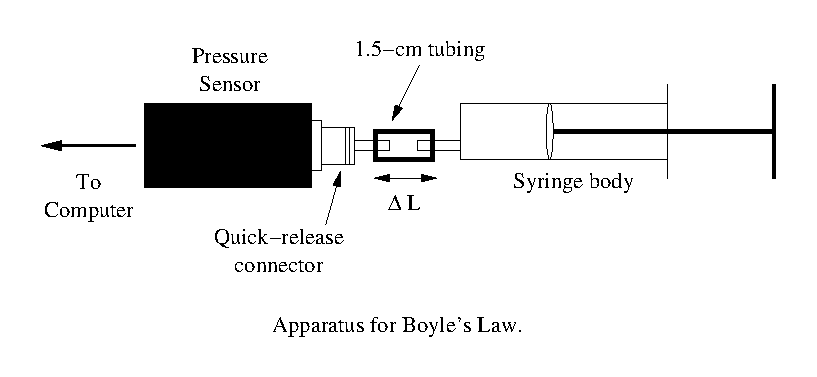
\includegraphics{boyles_law/boyleslawfig1.eps} \par}
\vspace{0.3cm}

\textbf{Introduction}

The behavior of a gas can be described in terms of the macroscopic quantities:
temperature (T), pressure (P), and volume (V). The relationship between these
quantities is given by the equation of state of the gas. A real gas behaves
approximately as an ideal gas if it is far from liquefaction. In that case,
the equation of state of an ideal gas can be used to describe a real gas. For
a given mass of a gas, if one of the quantities P, T, or V is changed, a change
in the other two quantities probably will result. However, if one of the quantities
is kept constant, the relationship between the other two can be studied. The
relationship between pressure and volume of an ideal gas is called Boyle's law.

The experimental apparatus is shown in the figure above. The gas is air contained
in a syringe that has marking on its side to measure the volume of the syringe.
A short tube connects the syringe with a pressure sensor that measures the pressure
in the tube and converts that measurement into a signal that can be read by
the DataStudio interface.

\textbf{Activity 1: Relationship Between P and V of a Gas}

(a) Check that there are no leaks in the apparatus by trying to compressing
the syringe from the 20.0 ml position to the 10.0 ml position. It should become
increasingly difficult to push the plunger as the volume decreases. If this
is not the case, check the couplings for fit. If no problem is obvious, then
consult your instructor. 
\vspace{20mm}

(b) The initial volume of air in the syringe should be set at 20.0 ml. If your
syringe is set to some other value, disconnect the quick release connector from
the sensor by gently rotating it in the counter-clockwise direction as you look
from the syringe toward the pressure sensor. Next, move the piston to the 20.0
ml position, and then re-connect the quick release connector to the pressure
sensor. 

(c) \textbf{Data Recording}. Open the Boyle's Law activity located in the 132
Workshop Folder under the {\bf Start} menu. Click on the window labeled \textit{Volume
and Pressure Table}. This is where your data will be displayed as you record
it. This table display will show the values of the gas volume in the syringe
which you will set by moving the piston to the appropriate marking on the syringe.
You will record the pressure at each of these settings with the pressure sensor.
To begin recording data, make sure the piston is at the 20-ml setting, and click
the Start button. The Start button will change to a Keep button and the table
display will show the value of the pressure next to the first volume value (20
ml) in the table. The reading in the pressure column should be colored red.
Click the Keep button to record this pressure (notice the reading in the Pressure
column beside the 20-ml entry changes from red to black). The next setting for
the volume (18 ml) will appear in the Volume column of the data table display.

NOTE: For the first pressure reading at 20 ml, the air in the syringe will be
in thermal equilibrium with the environment. This will not be the case immediately
after compressing the syringe for the next reading. Therefore, you must allow
a couple of seconds for the system to return to thermal equilibrium after you 
compress the syringe and before clicking on Keep to record pressure values. 

(d) Compress the syringe to the next value of the volume as listed in the data
display table (i.e., the window labeled \textit{Volume and Pressure Table})
and wait a couple of seconds for the system to reach thermal equilibrium. Once 
thermal equilibrium is reached, click Keep to record the pressure. The data 
table display will automatically change to show the next value of the volume 
at which the pressure will be measured. 

(e) Repeat step (d) for the remaining values of the volume listed in the table
display. In other words, continue taking pressure measurements at the prescribed
volume values in the data table display by moving the piston to the prescribed
value and clicking on Keep after thermal equilibrium is reached. After you record
the pressure for the last volume (8 ml), click the small, red box next to the
Keep button (this is the stop button) to end data recording.

(f) \textbf{Analysis.} What happened to the pressure when the volume was 
reduced from 20 ml to 8 ml? From looking at the data, do the pressure and 
volume seem to be directly or inversely proportional? Explain.
%Click on the GraphDisplay to examine the plots of Syringe
%Volume Reading vs. Pressure, and the Volume to Pressure ratio (as a function
%of measuring time). Print the GraphDisplay and attach it to this unit.
\vspace{25mm}

(g) Copy your data into a spreadsheet and plot pressure versus volume 
(including a title and axis labels with units). Next, fit your data with a 
trendline using a power function. Record the result here. What is the power of 
V? Print the graph and include it with this unit.
%What should you get for the power? Why?
\vspace{25mm}

(h) If pressure and volume are inversely proportional, then what can you say
about the product of pressure and volume? Explain.
\vspace{25mm}

\newpage

(i) The measurements you have made are V in milliliters (ml) and P in 
kilopascals (kPa). What are the corresponding units of PV? Show how you get 
this here (the result must be in energy units):
\vspace{40mm}

(j) Construct a table in the space below with the column headings: V (ml), P
(kPa), and PV. Include the units from above in the last column.
Enter the results for P and V in this new table and calculate
PV for each set of readings. Determine the mean value and the standard deviation
\( \sigma  \) for PV. Record the results in the form 
PV = Mean \( \pm \, \sigma  \). Be sure to include the proper units. 
What does this result tell you about the  product PV?

\vspace{12cm}

(k) Is there a trend in the values of PV as the volume decreases? If so, 
what do you suppose causes that trend?

%(j) Examine the plot on the next page with results from two different data 
%runs. How do you explain the difference between the curves for the different 
%tubing lengths (\( \triangle L \) in the diagram on the next page)?

%\vspace{40mm}

%\eject

%\vspace{0.3cm}
%{\par\centering 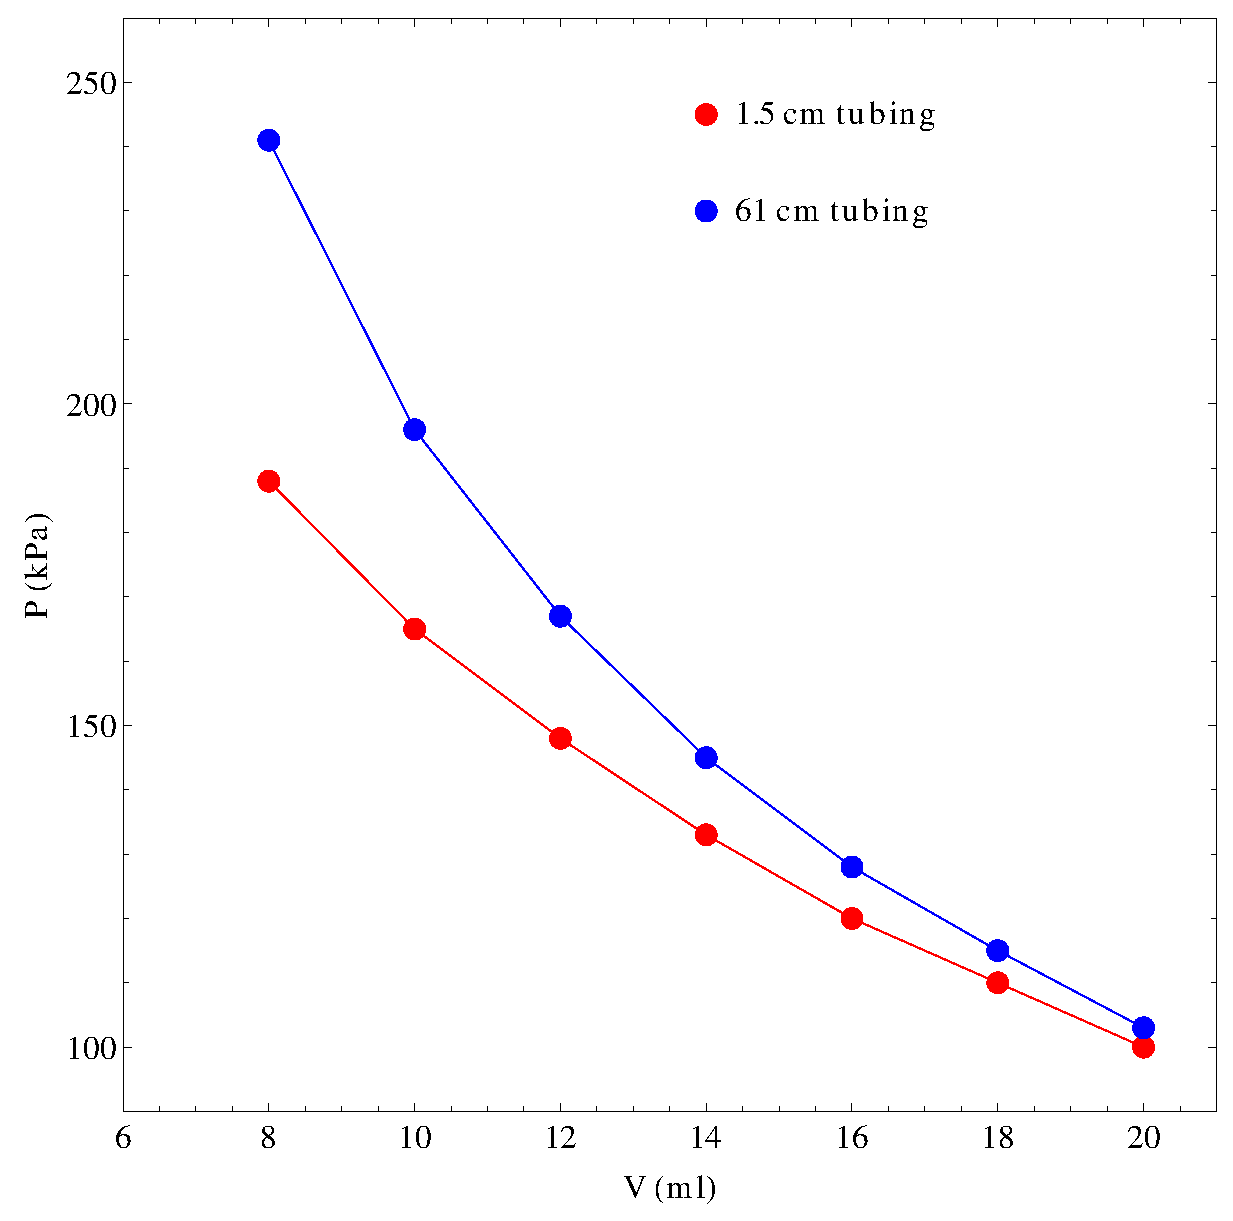
\includegraphics[width=6in]{boyles_law/PVfor132.eps} \par}
%\vspace{0.3cm}

%{\par\centering Results of measurement with Boyle's Law apparatus \par}

%{\par\centering different values of \( \triangle L \), the tubing length.\par}




\section{Charles' Law}

Name \rule{2.0in}{0.1pt}\hfill{}Section \rule{1.0in}{0.1pt}\hfill{}Date
\rule{1.0in}{0.1pt}+

\textbf{Objectives} 

To investigate the relationship between volume and temperature for
a constant mass of gas at constant pressure and determine the value
of absolute zero.

\textbf{Apparatus} 

\begin{itemize}
\item Charles law apparatus with stand.
\item Temperature sensor.
\item Air chamber, tubing, and ballast.
\item Containment vessel.
\end{itemize}
\vspace{0.3cm}

\begin{figure}[hbt]
\begin{center}
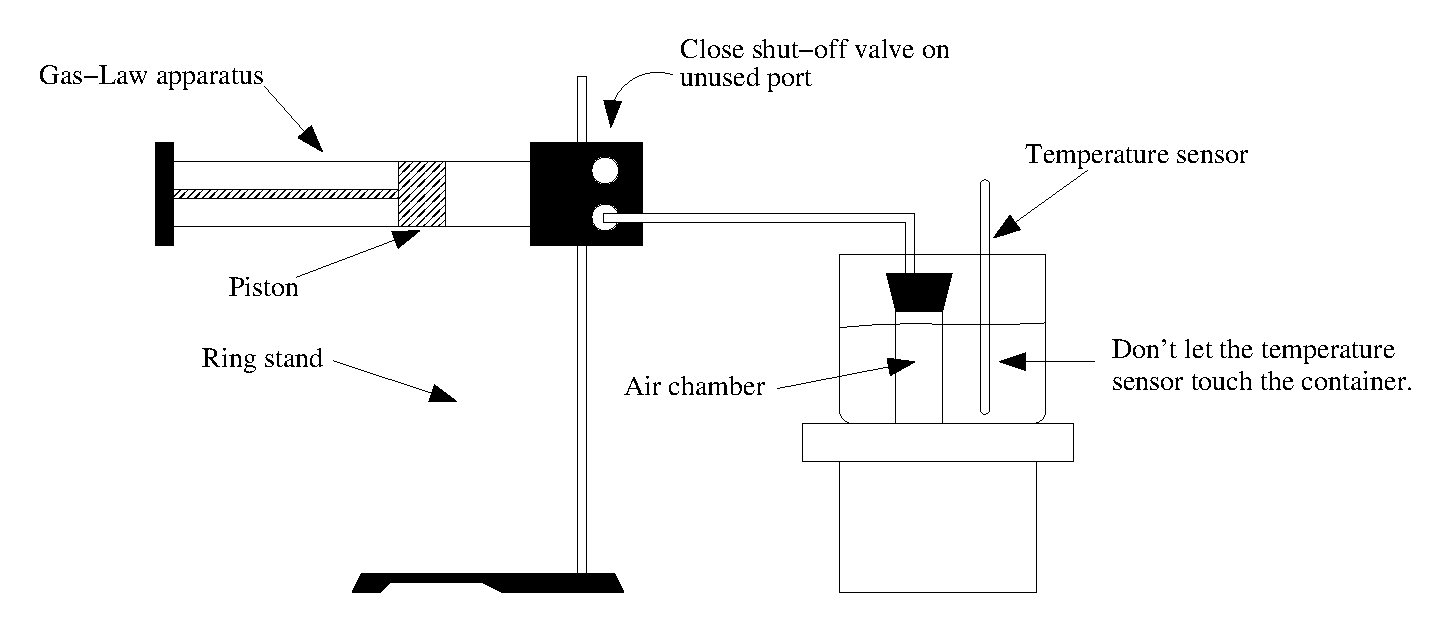
\includegraphics[width=6.0in]{charles_law_fig1.eps}
\caption{Charles' Law apparatus.}
\end{center}
\end{figure}

\textbf{Introduction}

The behavior of a gas can be described in terms of the macroscopic quantities:
temperature (T), pressure (P), and volume (V). The relationship between these
quantities is given by the equation of state of the gas. A real gas behaves
approximately as an ideal gas if it is far from liquefaction. In that case,
the equation of state of an ideal gas can be used to describe a real gas. For
a given mass of a gas, if one of the quantities P, T, or V is changed, a change
in the other two quantities probably will result. However, if one of the quantities
is kept constant, the relationship between the other two can be studied. The
relationship between temperature and volume of an ideal gas is called Charles' law.

The experimental apparatus is shown in the figure above and consists
of an air chamber containing dry air. The pressure on the air in the chamber is due to atmospheric
pressure applied through the movable piston.

\textbf{Activity 1: V-T Relationship for a Gas}

(a) Check that there are no leaks in the apparatus by trying to compressing
the piston from the 100 mm position to the 10 mm position. It should become
increasingly difficult to push the plunger as the volume decreases. If this
is not the case, check the couplings for fit. If no problem is obvious, then
consult your instructor. 

(b) Open the {\it Charles' Law} activity in the 132 Workshop Folder under the
{\bf Start} menu.
Click on the window labeled \textit{Charles' Law Table}. 
This is where your data will be displayed as you record
it. This table display will show the values of the gas temperature in the air chamber
and the entry number.
The data-taking procedure you will follow is described here first.
One member of your team will heat the air chamber in the flask on the hot plate 
and call out the position of the piston.
Another member will record the position settings by hand in the table below
and
click the {\bf Keep} button on the {\it DataStudio} interface to record the 
temperature for that entry.
To begin recording data, make sure the piston is at the low end of the scale, and click
the {\bf Start} button on the {\it DataStudio} interface. 
The {\bf Start} button will change to a {\bf Keep} button and the table
display will show the value of the temperature next to the first entry in the table. 
The reading in the temperature column should be colored red.
Click the {\bf Keep} button to record this temperature (notice the reading in the Temperature
column beside the entry number changes from red to black). The next entry number
 will appear in the Entry column of the data table display.

%NOTE: For the first temperature reading, the air in the chamber will be
%in thermal equilibrium with the environment. This will not be the case immediately
%after adding ice for the next reading. Therefore, you must allow
%3-5 seconds for the system to return to thermal equilibrium after you add ice
% and before clicking on {\bf Keep} to record temperature values. 

(c) Now, immerse the air chamber in a beaker of cold, tap water water and click
{\bf Start} on the {\it DataStudio} interface. You can monitor the temperature
on the temperature versus time plot to the right.
Make sure the set screw on the side of the piston is released.

(d) When the temperature is stable click {\bf Keep} and that point will be recorded in the
table. One team member should read off the piston position while the other 
writes it in the table at the same time.

(e) Now turn up the heat. The piston will move as the gas expands.
Read out the position of the piston every one or two millimeters. The other team member
will click {\bf Keep} (recording the temperature) and record the piston position
in the table.

(f) Repeat step (e) until the piston no longer moves or the water starts to boil.
 
(g) Calculate the volume of the apparatus for each piston position and plot
this volume versus temperature. The diameter of the Gas-Law apparatus is written on its
base.

\vspace{0.3cm}
{\centering \begin{tabular}{|c|c|c|c|}
\hline 
~~~Entry Number~~~&
~~~Piston Position (mm)~~~&
~~~Gas-Law Apparatus Volume (ml)~~~&
~~~Temperature ($^\circ  \rm C$)~~~\\
\hline
\hline 
&
&
&
\\
\hline 
&
&
&
\\
\hline 
&
&
&
\\
\hline 
&
&
&
\\
\hline 
&
&
&
\\
\hline 
&
&
&
\\
\hline 
&
&
&
\\
\hline 
&
&
&
\\
\hline 
&
&
&
\\
\hline
&
&
&
\\
\hline
&
&
&
\\
\hline
&
&
&
\\
\hline
&
&
&
\\
\hline
&
&
&
\\
\hline
\end{tabular}\par}
\vspace{0.3cm}

(h) How are the volume and temperature related?
Fit your data with the appropriate function and record the results here.
Print your plot and attach it to this unit.
\vspace{15mm}

(h) Repeat steps c-h to obtain a second {\it V-T} curve. Record your data in the table below
along with the fit to the V-T data.
\vspace{30mm}


\vspace{0.3cm}
{\centering \begin{tabular}{|c|c|c|c|}
\hline 
~~~Entry Number~~~&
~~~Piston Position (mm)~~~&
~~~Gas-Law Apparatus Volume (ml)~~~&
~~~Temperature ($^\circ  \rm C$)~~~\\
\hline
\hline 
&
&
&
\\
\hline 
&
&
&
\\
\hline 
&
&
&
\\
\hline 
&
&
&
\\
\hline 
&
&
&
\\
\hline 
&
&
&
\\
\hline 
&
&
&
\\
\hline 
&
&
&
\\
\hline 
&
&
&
\\
\hline
&
&
&
\\
\hline
&
&
&
\\
\hline
&
&
&
\\
\hline
&
&
&
\\
\hline
&
&
&
\\
\hline
\end{tabular}\par}
\vspace{2.0cm}

\textbf{Activity 2: Absolute Zero and the Kelvin Scale}

(a) The absolute zero of temperature can be defined as the temperature
at which the volume of an ideal gas is zero. Determine absolute
zero from the equations you obtained by fitting your V-T data.
\vspace{30mm}

(b) Determine the percent difference between your value of absolute
zero and the accepted value of -273\( ^{\circ } \)C. Are you happy or sad?
\vspace{30mm}

(c) Record the results from the other groups in class.
Obtain an average and standard deviation and record it here.
Are your results consistent with the class average? Explain.




\section{The \textit{P-T} Relationship of a Gas}

\makelabheader %(Space for student name, etc., defined in master.tex)

\bigskip
\textbf{Objectives} 

To investigate the relationship between pressure and temperature for
a constant mass of gas at constant volume and determine the value
of absolute zero.

\bigskip

\textbf{Apparatus} 

\begin{itemize}[nosep]
\item Pressure sensor
\item Temperature sensor
\item Air chamber and tubing
\item Hot plate
\item Glass beaker
\item Clamp and stand
\item Plastic beaker
\item Pasco 550 interface
\item \textit{Capstone} software (\filename{P-T.cap} experiment file)
\end{itemize}
\vspace{0.3cm}

\begin{figure}[hbt]
\begin{center}
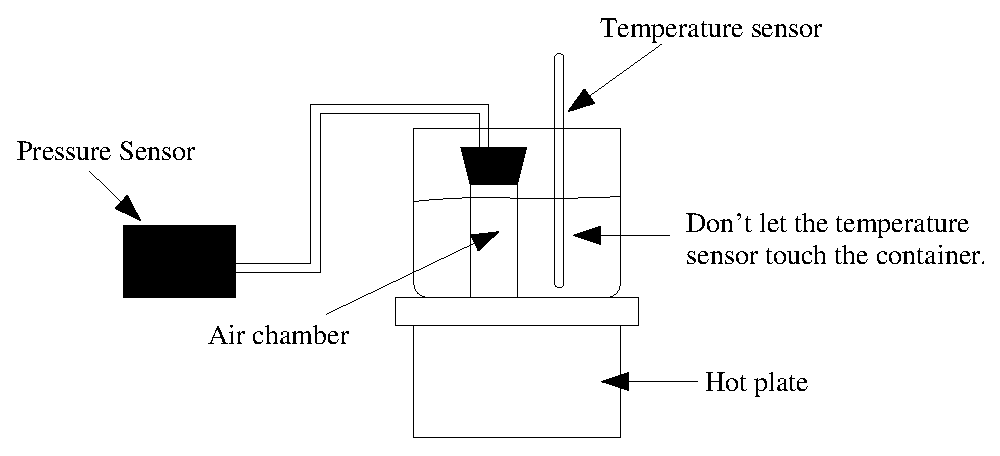
\includegraphics[width=6.0in]{P-T_relationship_of_gas/P-T_fig1b.eps}
\caption{P-T apparatus.}
\end{center}
\end{figure}

\textbf{Introduction}

The behavior of a gas can be described in terms of the macroscopic quantities:
temperature $T$, pressure $P$, and volume $V$. The relationship between these
quantities is given by the equation of state of the gas. A real gas behaves
approximately as an ideal gas if it is far from liquefaction. In that case,
the equation of state of an ideal gas can be used to describe a real gas. For
a given mass of a gas, if one of the quantities $P$, $T$, or $V$ is changed, a change
in the other two quantities probably will result. However, if one of the 
quantities is kept constant, the relationship between the other two can be 
studied. The relationship between temperature and pressure of an ideal gas is 
known as Gay-Lussac's law.

The experimental apparatus is shown in the figure above and consists
of an air chamber containing dry air. The volume of the gas is fixed. 
The temperature and pressure sensors are connected to the 550 Interface. 
Be sure the temperature sensor is connected to port A and the pressure sensor 
to port B. \textbf{Important:} Be sure the cables from the sensors are not touching the hot 
plate.

\bigskip

\pagebreak[2]
\textbf{Activity 1: $P$-$T$ Relationship for a Gas}

%(a) Fill the beaker 3/4 full with cold tap water and place it on the hot plate.  Immerse the air chamber in the water so that most of the volume of the air chamber is submerged.  The air chamber will have to be held in place with a clamp and stand or it will float to the top.  Set the temperature sensor in the water in such a way that it is not touching the side or bottom of the beaker.

(a) The equipment should be set when you arrive in lab. The air chamber is set 
inside the glass beaker on top of the hot plate. The temperature sensor is set 
so that it is not touching the side or bottom of the beaker. Use the plastic 
beaker to fill the glass beaker about 3/4 full of cold tap water.

(b) Open the file \filename{P-T.cap} in the \filename{\coursefolder} folder.
The graphs on the right display the temperature of the heat bath and the gas pressure as functions of time.  
The table on the left will record specific data points that you will choose.  
To begin recording data click
the \textit{Preview} button, which is where the \textit{Record} button usually would be. 
Once you hit \textit{Preview}, the current values of temperature and pressure will be coninuously graphed, and updated in the first row of the table.  When you hit the \textit{Keep Sample} button, the values at that time will be saved to the table, and you will continue to see current values displayed in the next row.


(c) Turn the hot plate on high.  As the temperature rises, click the \textit{Keep Sample} button when the temperature is 5-7\( ^{\circ } \) above its first value.  Continue recording the temperature and pressure at 5-7\( ^{\circ } \) intervals (by clicking the \textit{Keep Sample} button) until the water is close to boiling.  You can monitor the temperature on the temperature versus time plot to the right (on the monitor) or by watching the temperature in the \textit{Temperature and Pressure Table}.  After your last reading, click the \textit{Stop} button and turn off the hot plate.

(d) How are the pressure and temperature related?  Print your data table, enter the data in \textit{Excel} and plot pressure vs. temperature on a linear graph, showing the equation of the graph.  Print this graph and add it to this unit. Write the equation here as pressure $P$ as a function of temperature $T$, including UNITS on the constants.
\vspace{15mm}



\textbf{Activity 2: Absolute Zero and the Kelvin Scale}

(a) The absolute zero of temperature can be defined as the temperature
at which the pressure of an ideal gas is zero. Determine absolute
zero from the equation of your graph by setting $P = 0$ and solving for $T$.
\vspace{25mm}

(b) Record the results from the other groups in the class. 
Obtain an average and standard deviation and record it here.
Are your results consistent with the class average?  Explain.
\vspace{25mm}

(c) Does there appear to be a systematic error in the class results relative 
to the accepted value of $-273~^{\circ}$C?  If so, what do you suppose 
causes the error? Think about this and try to explain.





\setcounter{activity}{0}

\section{Impulse, Momentum, and Interactions\footnote{
1990-93 Dept. of Physics and Astronomy, Dickinson College. Supported by FIPSE
(U.S. Dept. of Ed.) and NSF. Portions of this material may have been modified
locally and may not have been classroom tested at Dickinson College.
}}
\setcounter{activity}{0}


\makelabheader %(Space for student name, etc., defined in master.tex)

\textbf{Objectives }

\begin{itemize}
\item To verify the relationship between impulse and momentum experimentally. 
\item To study the forces between objects that undergo collisions and other types of interactions in a short time period.
\end{itemize}
\textbf{Apparatus} 

\begin{center}
\begin{tabular}{|l|l|l|} \hline
Dynamics cart with flag and track   & Force probe   & Motion sensor \\ \hline
{\it Science Workshop 750 Interface}& compact scale & {\it DataStudio} \\ \hline
\end{tabular}
\end{center}

\textbf{The Impulse-Momentum Theorem }

When an object collides with something the force on it 'pushes' for a while and eventually
stops.
If the force $\vec F$ is constant, we can get some idea of the total `push' by multiplying by
the time $\Delta t$ the force acted.
This product is called the impulse $\vec I = \vec F \Delta t$ and it measures
the total 'kick' received by an object.
Real collisions, like those between eggs and hands, a Nerfball and a wall, or
a falling ball and a table top are tricky to study because $\Delta t$ 
is so small and
the collision forces are not really constant over the time the colliding objects
are in contact. Thus, we cannot calculate the impulse as $\vec F \,\Delta t$. 
Before we study
more realistic collision processes, let's redo the theory for a variable force.
In a collision, according to Newton's second law, the force exerted on a falling
ball by the table top at any infinitesimally small instant in time is given
by
\[
{\bf F}=\frac{d{\bf p}}{dt}\qquad [Eq.\: 1]\]


To describe a general collision that takes place between an initial time \( t_{i} \)
and a final time \( t_{f} \) , we must take the integral of both sides of the
equation with respect to time. This gives
\[
\int _{t_{i}}^{t_{f}}{\bf F}dt=\int _{t_{i}}^{t_{f}}\frac{d{\bf p}}{dt}dt=\left( {{\bf p}_{f}}-{{\bf p}_{i}}\right) =\Delta {\bf p}\qquad [Eq.\: 2]\]


Impulse is a vector quantity defined by the equation
\[
{\bf Area}=\int_{t_{i}}^{t_{f}}{\bf F}\,dt\qquad [Eq.\: 3]\]


By combining equations {[}2{]} and {[}3{]} we can formulate the impulse-momentum
theorem in which
\[
{\bf I}=\Delta {\bf p}\qquad [Eq.\: 4]\]


If you have a fairly smooth graph of how the force $F$ varies as a function
of time, the impulse integral can be calculated as the area under the $F$-$t$ 
curve.

Let's see qualitatively what an impulse curve might look like in a real collision
in which the forces change over time during the collision. In particular, let's
consider the collision of a Nerfball with a wall as shown below.

\vspace{0.3cm}
{\par\centering 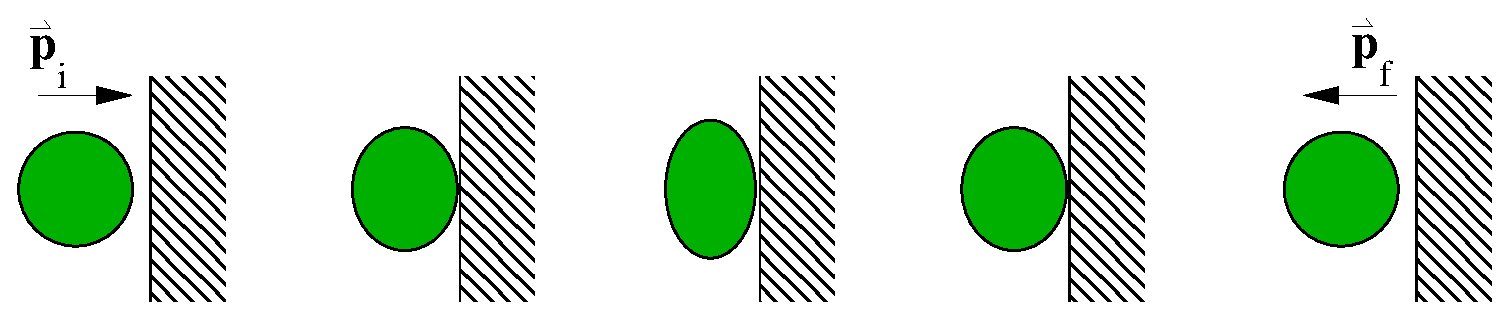
\includegraphics[width=5.0in]{impulseFor132/fig1.eps} \par}
\index{color page}
\vspace{0.3cm}

%\textbf{Activity  \stepcounter{activity}\arabic{activity}: Predicting Collision Forces That Change }
\textbf{Activity  1: Predicting Collision Forces That Change }

(a) Suppose a tennis ball is barreling toward a wall and collides with it. 
If friction is neglected, what is the net force exerted on the object just before it starts to collide?
\vspace{10mm}

(b) When will the magnitude of the force on the ball be a maximum? 
\vspace{10mm}

(c) Roughly how long does the collision process take? Half a second? Less? Several
seconds?
\vspace{10mm}

(d) Attempt a rough sketch of the shape of the force the wall exerts on a moving
object during a collision.

\vspace{0.3cm}
{\par\centering 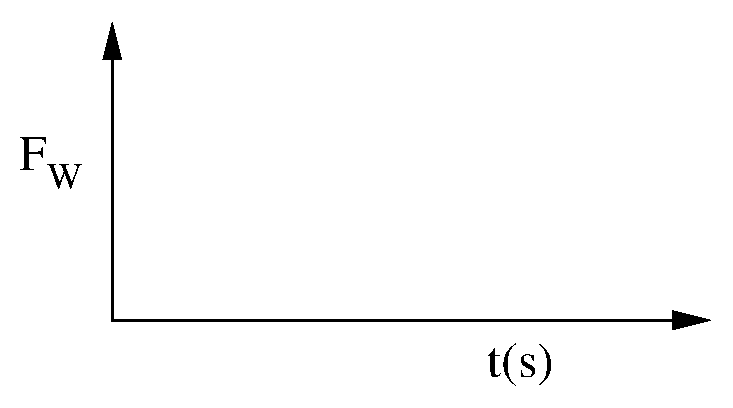
\includegraphics[width=2.5in]{impulseFor132/fig2.eps} \par}
\vspace{0.3cm}

\textbf{Verification of the Impulse-Momentum Theorem} 

To verify the impulse-momentum theorem experimentally we must show that for
an actual collision involving a single force on an object the equation
\[
\int_{t_{i}}^{t_{f}}{\bf F}\,dt=\Delta {\bf p}\]


holds, where the impulse integral can be calculated by finding the area under
the  $F$ \textit{vs.}~$t$ curve.

\vspace{0.3cm}
{\par\centering 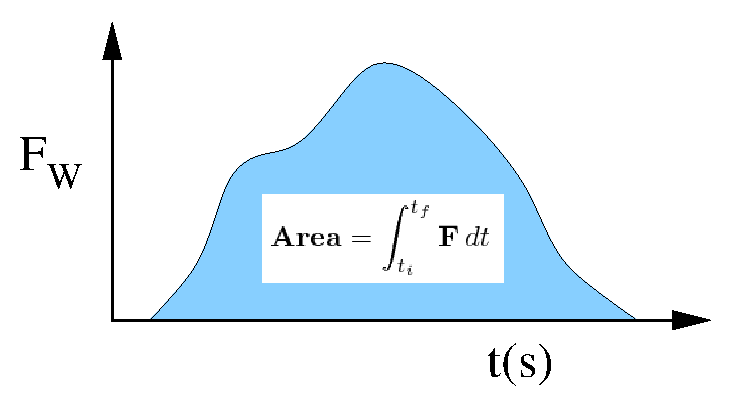
\includegraphics[width=2.5in]{impulseFor132/fig3.eps} \par}
\index{color page}
\vspace{0.3cm}

In this experiment you will investigate this theorem by measuring the impulse
and the change in momentum of a cart undergoing a one-dimensional collision.
The experimental setup is shown in the figure below. The end of the track with
the motion detector should be raised about 1.5 cm so that, when released, the
cart will collide with the force probe. The force probe will measure the force
as a function of time during the collision. The motion detector is used to measure
the velocity of the glider before and after the collision. You will use the
Impulse-Momentum application to make these measurements.

\vspace{0.3cm}
{\par\centering \resizebox*{0.9\textwidth}{!}{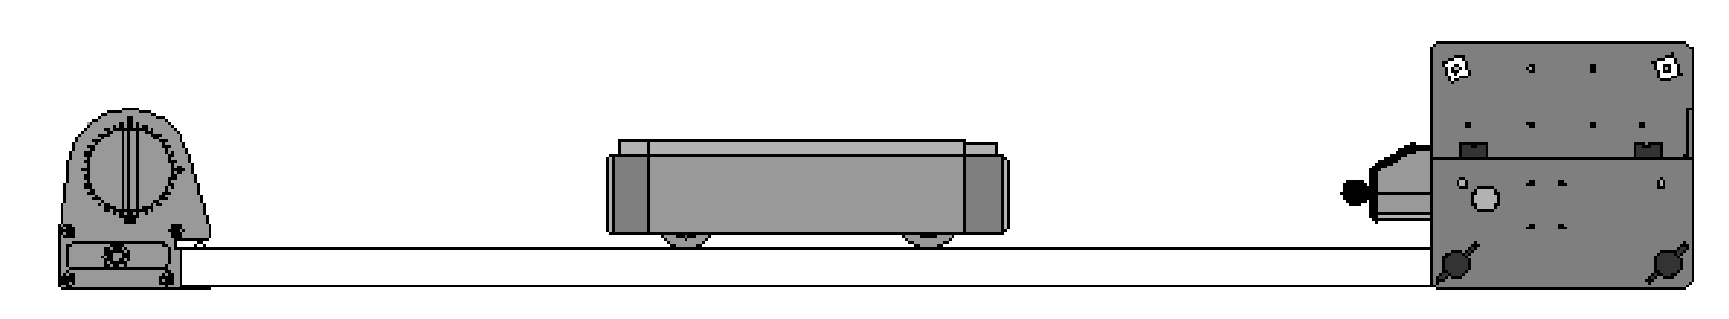
\includegraphics{impulseFor132/impulse_fig4.eps}} \par}
\vspace{0.3cm}

%\textbf{Activity  \stepcounter{activity}\arabic{activity}: Verification of the Impulse-Momentum Theorem} 
\textbf{Activity  2: Verification of the Impulse-Momentum Theorem} 

(a) Measure and record the mass of the cart, $m$, using the compact scale.
\vspace{10mm}

(b) Calibrate the force probe (see \textit{Calibrating Force Sensors} in \textbf{Appendix \ref{datastudio}: DataStudio}). 

(c) Construct a data table in the space below with the column headings Trial
\#, Area, \( v_{i} \), and \( v_{f} \). Make enough room to record five trials.

\begin{center}
\begin{tabular}{|p{1.0in}|p{1.0in}|p{1.0in}|p{1.0in}|} \hline
 & & & \\ \hline
 & & & \\
 & & & \\
 & & & \\
 & & & \\
 & & & \\
 & & & \\
 & & & \\
 & & & \\
 & & & \\
 & & & \\
 & & & \\
 & & & \\
 & & & \\ \hline
\end{tabular}
\end{center}

(d) Position the force probe part way up the track (to be closer to the motion sensor). Open the \textbf{Impulse-Momentum} application in the \textbf{131 Workshop} submenu. 

(e) Set the cart on the track about mid-way between the motion sensor and the force probe. Start recording data and release the cart. Stop recording data after the cart collides with the force probe and bounces back. The computer will then display graphs of velocity and force versus time.

(f) Determine the area under the force \textit{vs.}~time graph and record the value in
your data table. See \textbf{Appendix \ref{datastudio}: Introduction to DataStudio} for instructions on how to determine the area under a curve.

(g) Use the smart tool to find the velocity just before the collision and the
velocity just after the collision from the velocity versus time graph. Record
these values in your data table.

(h) Repeat parts (e) through (g). For these trials, 
the area function and the smart tool must be turned on and off for each trial. 
Print the graphs for one of your trials and include it with this report.

\newpage

(i) Construct another data table below with the column headings
Trial \#, $I$, \( \Delta  p\), Diff., and Percent diff. For each trial, calculate and record
the impulse, $I$, and the change in momentum, \( \Delta  p\), in kg\,m/s. Also,
determine the difference between $I$ and $\Delta p$  for each trial, and the percent difference. Also, show a sample
calculation of $I$ and \( \Delta  p\) for one of your trials.

\begin{center}
\begin{tabular}{|p{1.0in}|p{1.0in}|p{1.0in}|p{1.0in}|p{1.0in}|} \hline
 & & & & \\ \hline
 & & & & \\
 & & & & \\
 & & & & \\
 & & & & \\
 & & & & \\
 & & & & \\
 & & & & \\
 & & & & \\
 & & & & \\
 & & & & \\
 & & & & \\
 & & & & \\
 & & & & \\ \hline
\end{tabular}
\end{center}

(j) What do you expect for the values in the last column of your table (Percent diff)? Make a histogram of your results in that column and calculate the average and standard deviation. For information on making histograms, see \textbf{Appendix \ref{excel}}. For information on calculating the average and standard deviation, see \textbf{Appendix \ref{treatment}}. Record the average and standard deviation here.
Attach the histogram to this unit.
Is your data consistent with your expectation?  Be quantitative in your answer.
\vspace{20mm}

(k) Do your results verify the impulse-momentum theorem? Explain quantitatively.
\vspace{20mm}

(l) What does the histogram of your data tell you? Be quantitative in your answer.
\vspace{20mm}

(m) Is there any indication of a systematic uncertainty? What are the possible
sources of error?




\section{Kinetic Theory of Ideal Gases\footnote{%
1990-93 Dept. of Physics and Astronomy, Dickinson College. Supported
by FIPSE (U.S. Dept. of Ed.) and NSF. Portions of this material may
have been modified locally and may not have been classroom tested
at Dickinson College.
}}

Name \rule{2.0in}{0.1pt}\hfill{}Section \rule{1.0in}{0.1pt}\hfill{}Date
\rule{1.0in}{0.1pt}

\textbf{Objective} 

To derive a relationship between the macroscopic properties of an
ideal gas and the microscopic motion of the unseen atoms that make
up the gas. To do this activity you will need:

\begin{itemize}
\item A computer with an atomic and molecular motion simulation
\end{itemize}
\textbf{Introduction}

Do you believe in atoms? Our forefathers believed in the reality of
witches. In fact, they thought that they had good evidence that witches
existed, good enough evidence to accuse some people of being witches.
We believe in atoms. Are we truly more scientific than they were?

\textbf{Activity 1: Why Atoms!?}

(a) List reasons why you do or do not believe that matter consists
of atoms and molecules, even though you have never seen them with
your own eyes.
\vspace{20mm}

(b) What happens when heat energy is being transferred into a substance?
If you believe that substances are made of atoms and molecules, how
would you use their existence to explain the change in volume of a
heated gas?
\vspace{20mm}

\textbf{Models of Pressure Exerted by Molecules}

So far in physics we have talked about matter as if it were continuous.
We didn't need to invent aluminum atoms to understand how a ball rolled
down the track. But ever since the time of the fifth century B.C.
Greek philosophers Leucippus and Democritus, some thinkers have believed
in {}``atomism'', a picture of the universe in which everything
is made up of tiny {}``eternal'' and {}``incorruptible'' particles,
separated by {}``the void''. Today, we think of these particles
as atoms and molecules.

In terms of every day experience molecules and atoms are hypothetical
entities. In just the past 40 years or so, scientists have been able
to \char`\"{}see\char`\"{} molecules using electron microscopes and
field ion microscopes. But long before atoms and molecules could be
\char`\"{}seen\char`\"{} experimentally, nineteenth century scientists
such as James Clerk Maxwell and Ludwig Boltzmann in Europe and Josiah
Willard Gibbs in the United States used these imaginary microscopic
entities to construct models that made the description and prediction
of the macroscopic behavior of thermodynamic systems possible. Is
it possible to describe the behavior of an ideal gas that obeys the
first law of thermodynamics as a collection of moving molecules? To
answer this question, let's observe the pressure exerted by a hypothetical
molecule undergoing elastic collisions with the walls of a 3D box.
By using the laws of mechanics we can derive a mathematical expression
for the pressure exerted by the molecule as a function of the volume
of the box. If we then define temperature as being related to the
average kinetic energy of the molecules in an ideal gas, we can show
that kinetic theory is compatible with the ideal gas law and the first
law of thermodynamics. This compatibility doesn't prove that molecules
exist, but allows us to say that the molecular model would enable
us to explain the experimentally determined ideal gas law.

\textbf{Atomic Motion and Pressure}

Consider a spherical gas molecule that has velocity 
\( \overrightarrow{v}=v_{x} \)\( \hat{i}+v_{y} \)\( \hat{j} \)\( + v_z\hat k\) and
makes perfectly elastic collisions with the walls of a three-dimensional, cubical
box of length, width, and height $l$. Start the program called \char`\"{}\textit{Atoms
in Motion}\char`\"{}. You will see a screen
like the one shown below. Experiment with it for a few moments. 
The {\it Run} and {\it Stop} buttons control the processing of the 
simulation of the gas atoms while the {\it Step} button allows you to watch the
`movie' one frame at a time.

\begin{figure}[hbt]
\begin{center}
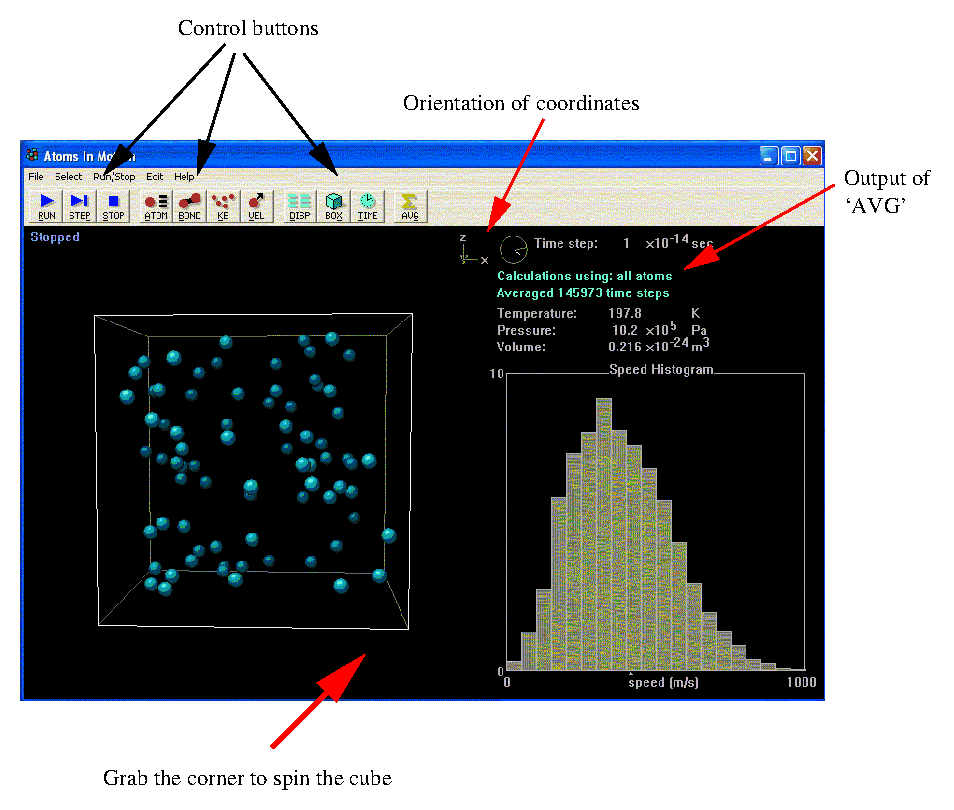
\includegraphics{am4a.eps}
\caption{{\it Atoms in Motion} window.}
\end{center}
\end{figure}

Can we use the concept of molecules behaving like little billiard
balls to explain why the ideal gas law relationship might hold? In
the next activity you are to pretend you are looking under a giant
microscope at a single spherical molecule as it bounces around in
a three-dimensional box by means of elastic collisions and that you
can time its motion and measure the distances it moves as a function
of time. 

If the molecule obeys Newton's Laws, you can calculate how the average
pressure that the molecule exerts on the walls of its container is
related to the volume of the box. The questions we have to consider
are the following. What is the momentum change as the
molecule bounces off a wall? How does this relate to the change in
the velocity component perpendicular to the wall? How often will our
molecule \char`\"{}hit the wall\char`\"{} as a function of its component
of velocity perpendicular to the wall and the distance between opposite
walls? What happens when the molecule is more energetic and moves
even faster? Will the results of your calculations based on mechanics
be compatible with the ideal gas law?

\textbf{Activity 2: The Theory of Atomic Motion}

(a) Stop the simulation if it's running and set the number of molecules to 
one. Do this by clicking on the {\it ATOM} button and getting a dialog box.
Enter `1' for the
number of Type A atoms and zero for all the others. Record the mass of the
Type A atom. Click {\it OK} and
the cube should now contain a single atom. If not, consult your instructor.
\vspace{20mm}

(b) The orientation of coordinates can be seen just about the right-hand corner
of the cube (consult Figure 1 also).
Suppose the molecule moves a distance $l$ in the $x$-direction in
a time \( \Delta t_{x} \). What is the equation needed to calculate
its $x$-component of velocity in terms of $l$ and \( \Delta t_{x} \)?
\vspace{20mm}

(c) Suppose the molecule moves a distance $l$ in the $y$-direction in
a time \( \Delta t_{y} \). What is the equation needed to calculate
its $y$-component of velocity in terms of $l$ and \( \Delta t_{y} \)?
\vspace{20mm}

(d) Suppose the molecule moves a distance $l$ in the $z$-direction in
a time \( \Delta t_{z} \). What is the equation needed to calculate
its $z$-component of velocity in terms of $l$ and \( \Delta t_{z} \)?
\vspace{20mm}

(e) We will now measure the average time $\Delta t_y$ for one complete round trip
from the left side of the cube to the right side and back again.
Click {\it AVG} and you will see some information printed in the color blue
on the right-hand side of the {\it Atoms-in-Motion} window (see also Figure 1).
The simulation takes small steps in time and calculates the positions of the
atoms at the end of each time step.
The number of these time steps taken is shown on the right-hand side and the size 
of each time step is printed at the top, right-hand-side of the window.
Using the {\it Step} button let the atom in the cube move until it bounces off the 
left wall of the cube.
Record the number of time steps in the space below.
\vspace{20mm}

(f) Now run or step the simulation until the atom bounces across the cube, hits the right-hand 
wall, comes back and strikes the left hand wall.
Record the number of time steps.
Calculate $\Delta t_y$ and record it below.
\vspace{20mm}

(g) Each side of the cube has a length $50 \times 10^{-10}$~m.
Combine this with the previous result to determine $v_y$ and record it.
\vspace{20mm}

(h) Repeat the above procedure for the top and bottom walls of the cube to get $v_z$.
\vspace{20mm}

(i) Rotate the cube by clicking and dragging one of the corners of the cube.
Spin it until you can see the atom bounces between the walls in the direction of
the $x$ coordinate.
Measure the $x$ component of the speed of the atom using the same procedure as before.
\vspace{20mm}

(j) Write the
expression for \( v_{total} \) in terms of the $x$, $y$, and $z$ components
of velocity. (Hint: This is an application of the 3-dimensional Pythagorean
theorem.) Determine $v_{total}$ for your atom.
We will use these results in a little while to calculate the pressure exerted by
our one-atom `gas'.
\vspace{20mm}

(k) Record the value of the pressure and temperature for your `gas'.
\vspace{20mm}

(l) We would like to eventually find the average kinetic energy of each atom or molecule
in a gas so we now have to think about a gas with many atoms.
Since the kinetic energy of a molecule is proportional to the square
of its total speed, you need to show that if \emph{on the average}
\( v_{x}^{2}=v_{y}^{2}=v_{z}^{2} \), then \( v_{total}^{2}=3v_{x}^{2} \).
\vspace{20mm}

(m) If the collisions with the wall perpendicular to the $x$ direction
are elastic, show that the force exerted on that wall for each collision
is just \( F_{x}=2m\frac{v_{x}}{\Delta t_{x}} \)where m is the mass
of the particles and \( \Delta t_{x} \) the mean interval between
collisions with the wall. (Hint: Think of the form of Newton's second
law in which force is defined in terms of the change in momentum per
unit time so that \( F=\frac{\Delta p}{\Delta t} \).)

\textbf{Warning:} Physicists too often use the same symbol to stand
for more than one quantity. In this case, note that \( \Delta p \)
(where {}``p'' is in lower case) indicates the change in \emph{momentum},
not pressure.
\vspace{20mm}

(n) Substitute the expression from part (b) for \( \Delta t_{x} \)
to show that 

\[
F_{x}=\frac{mv_{x}^{2}}{d}\]

\vspace{20mm}

(o) For simplicity, let us assume that we have a cubical box so that
\( x=y=z=L \), where L is the length of a side of the cube. Show
that the pressure on the wall perpendicular to the x axis caused by
the force \( F_{x} \) due to \emph{one} molecule is described by
the following expression.

\[
P=\frac{mv_{x}^{2}}{L^{3}}\]

\vspace{20mm}

(p) Let's say that there are not one but N molecules in the box. What
is the pressure on the wall now?
\vspace{20mm}

(q) Next, show that if we write the volume of our box as \( V=L^{3} \),
and recalling that

\[
v_{x}^{2}=\frac{v_{total}^{2}}{3}\]


we can write the following expression.

\[
P=N\frac{mv_{total}^{2}}{3V}\]

\vspace{20mm}

(r) Finally, since the average kinetic energy of a molecule is just

\[
<E_{kin}>=\frac{1}{2}mv_{total}^{2}\]


show that the pressure in the box can be written in the following
way.

\[
P=\frac{2N<E_{kin}>}{3V}\]
\vspace{20mm}

(s) Use the previous result to calculate the pressure using $v_{total}$, the mass of the
atom, $N$ and $V$ for your one-atom gas. Compare your result with the pressure you recorded above from the
output of the simulation.
Do they agree?
Explain any differences.
\vspace{20mm}



\section{Applying the Kinetic Theory\footnote{%
1990-93 Dept. of Physics and Astronomy, Dickinson College. Supported
by FIPSE (U.S. Dept. of Ed.) and NSF. Portions of this material may
have been modified locally and may not have been classroom tested
at Dickinson College.
}}

\makelabheader %(Space for student name, etc., defined in master.tex)

\textbf{Objective}

To derive the relationship between temperature and the kinematic properties
of the monatomic molecules of an ideal gas. We will also calculate
the specific heat per mole of an ideal, monatomic gas at constant
volume using the kinetic theory and compare the prediction with data.
To do this activity you will need:

\begin{itemize}
\item A computer with an atomic and molecular motion simulation
\end{itemize}

\textbf{Kinetic Energy, Internal Energy, and Temperature}

We have hypothesized the existence of non-interacting molecules to
provide the basis for a particle model of ideal gas behavior. We have
shown that the pressure of such a gas can be related to the average
kinetic energy of each molecule:

{\centering \( P=\frac{2N\left\langle E_{kin}\right\rangle }{3V} \)
or \( PV=\frac{2}{3}N\left\langle E_{kin}\right\rangle  \)\par}

Pressure increases with kinetic energy per molecule and decreases
with volume. This result makes intuitive sense. The more energetic
the motions of the molecules, the more pressure we would expect them
to exert on the walls. Increasing the volume of the box decreases
the frequency of collisions with the walls, since the molecules will
have to travel longer before reaching them, so increasing volume should
decrease pressure if \( \left\langle E_{kin}\right\rangle  \) stays
the same.

\textbf{The Molar Specific Heat}

The kinetic theory of gases uses the atomic theory to relate the macroscopic
properties of gases to the microscopic features of the atoms and molecules
that make up the gas. In this laboratory we will extend the calculations
that we have made so far to include the molar specific heat of an
ideal, monatomic gas. The success of that extension of the theory
depends on how well the calculations reproduce the measured heat capacities
of a variety of real (not ideal) gases.

\textbf{Activity 1: Experimenting with the Gas Simulation Program}

Open the {\it Atoms in Motion} program (in {\it Physics Applications}) on the {\it Start} menu.
%(You will need to run it on a ``virtual machine''; see Appendix \ref{virtual_machine}.)  
We are first going to explore the relationship between pressure and volume in
our kinetic theory using the simulation. 

(a) According to the ideal gas law \( PV = nRT = Nk_{B}T \), where \( R \) is the universal gas constant and \( k_{B} \) is Boltzmann's constant. What
should happen to the pressure of an ideal gas as its volume increases
or decreases?
\vspace{1.0in}

(b) We now want to run a more realistic simulation.
Under the \button{ATOM} menu set the number of Type A atoms to 50 and set all the others to zero.
Click on the \button{BOX} button and a new dialog box will appear.
Check the box beside \button{Floor conducts heat} and set the temperature to $200$~K.
Notice at the top that the box width is $l=50 \times 10^{-10}$~m.
We have now set up a situation where one side of the cube is held at a constant
temperature (\textit{e.g.} it's sitting on a stove) so the collisions of the atoms with the
floor are no longer elastic.
The remaining sides of the
cube do not transfer any energy (they're insulated) so elastic collisions still occur 
at those walls.

Start
the simulation and make sure you are averaging the pressure over many time steps.
You should see the number of averaged time steps increasing on the right-hand side 
of the \button{Atoms-in-Motion} window. 
If you don't see this information, click on \button{AVG} and it should appear.

\newpage

(c) What happens to the pressure?
What happens to the temperature of the gas? 
You will find that it can take several minutes of computer time for the temperature of the gas to reach equilibrium with the floor.
Once the gas temperature is within 8 -- 10~K of the floor temperature, we can consider the gas and the floor to be in thermal equilibrium. Record the volume, pressure and temperature of the gas in the first line of the table below.
\vspace{20mm}

(d) Record the volume, pressure and temperature of the gas for five more volumes of the cube. Change the volume of the cube using the \button{BOX} menu and 
increasing the box width in increments of $10 \times 10^{-10}$~m. The volume 
is printed on the \button{Atoms-in-Motion} window. In each case, wait until the
temperature is within 8 -- 10~K of the floor temperature (the closer the better).
Plot your results including a trend line with a power function and attach the 
graph to this unit. Are your results consistent with the ideal gas law and
your prediction in part~(a)? 
%Are they consistent with the results of Experiment \ref{lab_boyles_law} (Boyle's law)?
%\vspace{1.5in}

\vspace{0.3cm}
{\renewcommand{\arraystretch}{1.2}
{\centering \begin{tabular}{|C{1.3in}|C{1.3in}|C{1.3in}|}
\hline 
Volume of Box &
Average Pressure &
Temperature \\
\hhline{|=|=|=|}
& &
\\
\hline 
& &
\\
\hline 
& &
\\
\hline 
& &
\\
\hline 
& &
\\
\hline 
& &
\\
\hline
\end{tabular}\par}}
\vspace{0.3cm}

(e) In the procedure above you should have found the pressure to be inversely
proportional to the volume. How could you modify your plot to show
the pressure is proportional to \( 1/V \)? Make such a plot and fit it with a 
linear function. How close is your data to following a straight line? Attach 
the plot to this unit.
\vspace{1.4in}

(f) According to the ideal gas law \( PV = nRT = Nk_{B}T \). What
should happen to the pressure of an ideal gas as the number of particles
increases or decreases?
We will explore this idea with the simulation next.
\vspace{1.4in}

(g) Start off with the gas parameters from the last `run' of the 
simulation.
Record the number of atoms, temperature, and pressure in the table below.
Use the \button{ATOM} menu to change the number of atoms (or molecules) in the cube.
Start
the simulation. What happens to the pressure? Record the pressure
and the number of molecules for four more values of the number of
molecules and plot your results. Attach the plot to this unit. Are your results consistent with
the ideal gas law and your prediction in part (f)?
\vspace{1.5in}

\vspace{0.3cm}
{\renewcommand{\arraystretch}{1.2}
{\centering \begin{tabular}{|C{1.5in}|C{1.3in}|C{1.3in}|}
\hline 
Number of Molecules&
Average Pressure&
Temperature\\
\hhline{|=|=|=|}
& &
\\
\hline 
& &
\\
\hline 
& &
\\
\hline 
& &
\\
\hline 
& &
\\
\hline
\end{tabular}\par}}
\vspace{0.3cm}

\textbf{Kinetic Theory and the Definition of Temperature}

The model of an ideal gas we have just derived requires that

{\centering \( PV=\frac{2}{3}N\left\langle E_{kin}\right\rangle  \)\par}

But we have determined experimentally the ideal gas law:

{\centering \( PV = Nk_{B}T \)\par}

What can we say about the average kinetic energy per molecule for
an ideal gas? You can derive a relationship between temperature and
the energy of molecules that serves as a microscopic (i.e. molecular)
definition of temperature.

\pagebreak[2]
\textbf{Activity 2: Microscopic Definition of Temperature}

(a) From the two equations above, derive an expression relating \( \left\langle E_{kin}\right\rangle  \)
and \( T \). Show the steps in your derivation.
\vspace{1.5in}

(b) In general, molecules can store energy by rotating or vibrating,
but for an ideal gas of \emph{point} particles (monatomic gas), the only possible form of kinetic energy is the translational motion of the particles. If we can ignore potential energy due to gravity or electrical forces, then the internal
energy \( E_{int} \) of a gas of \( N \) particles is \( E_{int}=N\left\langle E_{kin}\right\rangle  \).
Use this and the formulas above to show that for an ideal gas of point particles, $E _{int}$
\emph{depends only on N and T}. Derive the equation that relates \( E_{int} \),
\( N \) and \( T \). Show the steps.
\vspace{1.5in}

The microscopic and the macroscopic definitions of temperature are
equivalent. The microscopic definition of temperature which you just
derived is fundamental to the understanding of all thermodynamics!

\pagebreak[2]
\textbf{Activity 3: Calculating the Molar Specific Heat}

In this section we will generate a series of equations that we will
then bring together in order to predict the molar specific heat at
constant volume.

(a) Consider an ideal gas in a rigid container that has a fixed volume.
How is the molar specific heat defined in terms of the heat added \( Q \)?
\answerspace{1in}

(b) If the gas is heated by an amount \( Q \), then how much work is done
against the fixed container? Recall the first law of thermodynamics
and incorporate this result into your statement of the first law.
\answerspace{1in}

(c) Now use the equations of parts (a) and (b) to relate the change
in internal energy \( \Delta E_{int} \) to the molar specific heat.
\answerspace{1in}

%(d) We now want to find another expression for the change in internal
%energy \( \Delta E_{int} \) that is related to the average kinetic
%energy of the particles in the gas. How do you think the internal
%energy of an ideal, monatomic gas is related to \( \left\langle E_{kin}\right\rangle  \)
%(notice you are calculating the internal energy \( E_{int} \) here,
%not \( \Delta E_{int} \))?
%\vspace{1in}

(d) Write down an expression for  the change in internal
energy of the ideal gas in terms of \( \left\langle E_{kin}\right\rangle  \).
(Suggestion: see part (b) of Activity 2.)
How is \( \left\langle E_{kin}\right\rangle  \) related to the temperature?
Incorporate this relationship into your expression for the change
in the internal energy. You should find that

{\centering \( \Delta E_{int}=\frac{3}{2}Nk_{B}\Delta T \)\par}

where \( k_{B} \) is Boltzmann's constant and N is the number of
molecules in the gas.
\answerspace{1in}

(e) Use the equations is parts (c) and (d) to relate the molar specific
heat to the number of particles \( N \) and Boltzmann's constant \( k_{B} \).
You should find that

{\centering \( nC_{V}=\frac{3}{2}Nk_{B} \)\par}

where \( n \) is the number of moles.
\answerspace{1.5in}

\pagebreak
(f) How is the number of molecules in the gas \( N \) related to the number
of moles \( n \) and Avogadro's number \( N_{A} \)? Use this expression
and the result of part (e) to show \nopagebreak

{\centering \( C_{V}=\frac{3}{2}N_{A}k_{B} \) or \( \frac{C_{V}}{N_{A}k_{B}}=\frac{3}{2} \)\par} 
\answerspace{1.5in}

Since \( N_{A}k_{B}=R \), this can be written as

{\centering \( C_{V}=\frac{3}{2}R \) or \( \frac{C_{V}}{R}=\frac{3}{2} \)\par}
\vspace{0.3in}

\textbf{Activity 4: Comparing Calculations and Data}

We now want to compare our calculation of the molar specific heat
of an ideal, monatomic gas with the measured molar specific heats
of some real gases. The table below lists some of those measurements.

{\renewcommand{\arraystretch}{1.2}
{\centering \begin{tabular}{|c|c|c|c|}
\hline 
Molecule&
\( \frac{C_{V}}{R} \)&
Molecule&
\( \frac{C_{V}}{R} \)\\
\hhline{|=|=|=|=|}
He&
1.50&
CO&
2.52\\
\hline 
Ar&
1.50&
Cl\( _{2} \)&
3.08\\
\hline 
Ne&
1.51&
H\( _{2} \)O&
3.25\\
\hline 
Kr&
1.49&
SO\( _{2} \)&
3.77\\
\hline 
H\( _{2} \)&
2.48&
CO\( _{2} \)&
3.42\\
\hline 
N\( _{2} \)&
2.51&
CH\( _{4} \)&
3.25\\
\hline 
O\( _{2} \)&
2.53&
&
\\
\hline
\end{tabular}\par}}
\vspace{0.3cm}

(a) Has our theoretical calculation been successful at all? Which
gases appear to be consistent with our calculation? Which gases are
not? How do these two groups of real gases differ?
\answerspace{1in}

(b) Can you suggest an explanation for the partial success of the
theory? Which one of the original assumptions that went into our kinetic
theory might be wrong? (See Activity 2(b).)
\answerspace{2in}



\section{Einstein Solid}

\makelabheader %(Space for student name, etc., defined in master.tex)

\textbf{Objective}

To develop a quantum-mechanical model of an elemental solid ({\it e.g.} aluminum) and
introduce the ideas of statistical mechanics.

\textbf{Overview of the Model}

One of the earliest successful applications of quantum mechanics was done by Albert Einstein
in 1907 when he developed a model of an elemental solid ({\it i.e.} one that consists of a single
element from the periodic table like aluminum, lead, {\it etc.}).
We start by assuming that each atom in the solid is bound in a square lattice with each
of six neighbors. Each bond is treated as a simple spring so the 
mechanical energy for a single atom is
%\begin{wrapfigure}[16]{l}{3.0in}
%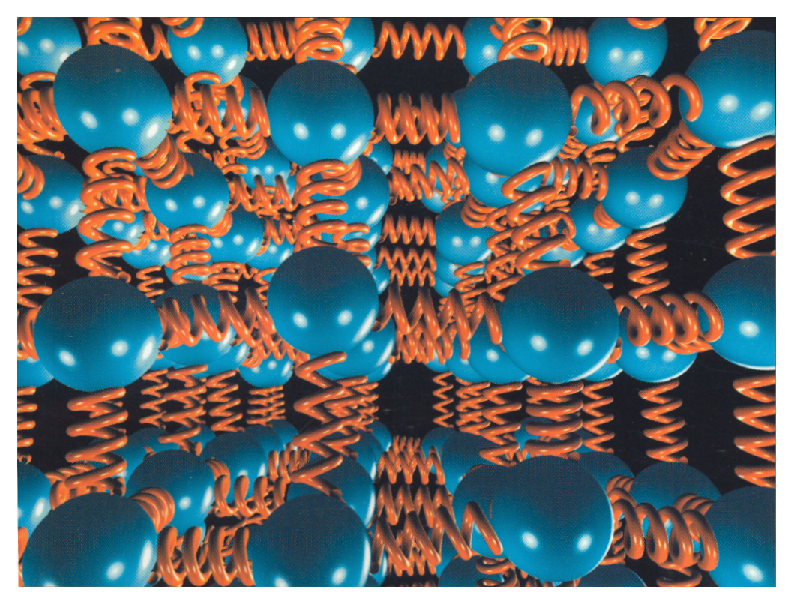
\includegraphics[height=2.0in]{einstein_solid/einstein_solid_picture2.eps}
%
%\hfil Fig. 1 Einstein solid.\hfil 
%
%\setcounter{figure}{1}
%
%\end{wrapfigure}
\begin{equation}
E = \frac{1}{2} m (v_x^2 + v_y^2 + v_z^2) + \frac{1}{2} k (x^2 + y^2 + z^2)
\end{equation}
where $k$ is the spring constant of the bond, the coordinates $x$, $y$, and $z$ are relative to the
equilibrium position of the atom and $v_x$, $v_y$, and $v_z$ are the components of the velocity.
Einstein used an idea pioneered by Max Planck in 1901 and
guessed the energy in the solid came in discrete pieces or quanta that were all
the same size.
Adding or removing these quanta heated or cooled the solid.
Many years later the quantum mechanical energy $E$ for a mass on a spring was found 
to be
\begin{equation}
E = (n_x + n_y + n_z + \frac{3}{2})\hbar \omega
\end{equation}
where $\hbar$ is Planck's constant, $\omega$ is related to the spring constant $k$ of the bond
mentioned
above, and $n_x$, $n_y$, and $n_z$ represent the number of quanta associated with each
degree of freedom of the spring.
The degrees of freedom here correspond to the three possible directions each atom can vibrate.
The size of each energy quantum is $\epsilon = \hbar \omega$.
The total number of energy quanta in the solid is labeled $q_A$ so the internal energy is
$E_{int} = q_A\epsilon$.
We then assume that all microstates of the solid have an equal probability of being populated.
A microstate is a specific arrangement of the quanta on the atoms in the solid.

\textbf{Activity 1: The Statistics of Matter}

Before you embark on building the model of the Einstein solid consider some ideas from
your previous study of gases. 
You will make some predictions here about the statistical nature of matter that you can
refer back to later on in this unit.

(a) Consider a gas in a container. Would it violate Newton's Laws or any other physical law
if all the particles in the gas collided in such a way that all of the gas particles
ended up in the bottom half of the container leaving the top half empty?
\vspace{15mm}

(b) Is such a scenario likely? Explain.
\vspace{15mm}

(c) If you started out with all the gas in the bottom half of the container how likely is
it to stay there?
\vspace{15mm}

The questions you answered above are addressing the notion of irreversibility.
Many processes in nature appear to proceed in one `direction' only.
When you add milk to coffee it disperses throughout the coffee.
After it is dispersed, the milk never re-concentrates into a blob of milk in the
middle of the coffee.
These processes go from a more orderly configuration (a concentrated drop of milk)
to a disordered state (milk spread throughout the liquid).
The reverse never happens.
We will return to this notion again in this laboratory.

\textbf{Activity 2: Calculating the Multiplicity of Some `Solids'}

(a) You will first calculate the configurations of 
the quanta (the microstates) for a VERY simple solid consisting of a single
atom!
The number of atoms for solid $A$ is $N_A=1$ so there are three degrees of
freedom $N_a=3$ because there is one degree of freedom for each
spatial direction.
The atom's vibration can be decomposed into three components, one for each direction.
Let the `solid' contain two quanta of energy so $q_A=2$.
Make a table with the headings $n_1$, $n_2$, and $n_3$ 
and in each row enter one
arrangement of the two quanta.
Each row in the table is a microstate.
Make a table with all of the possible microstates.
The multiplicity $\Omega_A$ of the system is the number of all possible
microstates. What is your multiplicity?
Record it here.
\vspace{45mm}

(b) You can calculate the multiplicity $\Omega_A$ using the expression
\begin{equation}
\Omega(N_A,q_A) = \frac{(q_A + 3N_A -1)!}{q_A! (3N_A-1)!}
\end{equation}
Make the calculation for $N_A = 1$ and $q_A = 2$.
Does this agree with your result in part 2.a?
\vspace{15mm}

(c) Now do the same thing for a different `solid'.
This time for solid $B$, let $N_B = 2$ (two whole atoms!) and $q_B = 1$.
How many degrees of freedom does solid $B$ have?
Make a table analogous to the one in part 2.a on the same sheet as before.
What is the multiplicity of solid $B$?
Record it here.
Use the expression in Activity 2.b to check your calculation.
\vspace{45mm}

\textbf{Activity 3: Putting the `Solids' Together}

When two solids are brought together heat/energy can flow between the two objects.
For the model of the Einstein solid you are building this corresponds to 
energy quanta ($\hbar \omega$) moving from atom to atom and occupying different
microstates of the combined system.

(a) Now bring the your solids $A$ and $B$ `together' into a single system.
What is $N_{AB}$ the total number of atoms?
What is the number of degrees of freedom of the combined system?
\vspace{10mm}

(b) What is the total number of energy quanta $q_{AB}$ for the combined system?
\vspace{10mm}

(c) The system is in its initial macrostate.
A macrostate is a configuration of the system defined here by the total number
of atoms and quanta in each solid.
In this case the macrostate is defined by $N_A=1$, $q_A=2$, $N_B=2$, and $q_B= 1$.
 What is the total multiplicity $\Omega_{AB}$ for the combined system
with $q_A=2$ and $q_B=1$ in its initial macrostate?
\vspace{15mm}

(d) Now take the energy quantum in solid $B$ and put it in solid $A$,
{\it i.e.}, let heat flow from solid $B$ into solid $A$.
This is now a macrostate where $q_A=3$ and $q_B=0$.
What is the new multiplicity $\Omega_A$ for solid $A$ and the  multiplicity $\Omega_B$ for solid $B$?
\vspace{20mm}

(e) What is the multiplicity $\Omega_{AB}$ for the combined system (solids $A$ and $B$)?
\vspace{15mm}

(f) Remember that a macrostate is defined by the combination of $N_A$, $N_B$, $q_A$, and $q_B$.
Which macrostate had the greatest multiplicity, $(q_A=2, ~ q_B=1)$ or $(q_A=3, ~ q_B=0)$
(remember that $N_A$ and $N_B$ are the same in each configuration so we don't 
list those parameters here)?
\vspace{15mm}

(g) If the energy quanta can move from atom to atom
which macrostate $(q_A=2, ~ q_B=1)$ or $(q_A=3, ~ q_B=0)$ is most probable? Why?
\vspace{15mm}

(h) If you started out in the $(q_A=3, ~ q_B=0)$ macrostate is it more likely that you will remain
in that macrostate of evolve to the $(q_A=2, ~ q_B=1)$ macrostate? Why?
\vspace{15mm}

What you have discovered is a version of the irreversibility mentioned earlier,
One macrostate ($q_A=2$, $q_B=1$) is preferred over the other because it has more microstates
than the other.
This result depends critically on your assumption that all states are equally populated.

\newpage

\textbf{Activity 4: Using {\it StatMech} For More Complex Cases}

You should have found in the previous activity that the $(q_A=2, ~ q_B=1)$ 
macrostate was more likely
to occur and the process proposed in part 3.d is relatively unlikely.
In other words, it is more likely for energy to be spread evenly throughout the system.
This is good news because it means the statistical picture we are painting is consistent
with reality.
Remember what happens to the blob of milk in the coffee.

(a) You should realize that making the sorts of calculations you did in Activity 3 above would
become rather painful for say $N_A = 300$ atoms.
In order to push the model further you will use a software packaged called 
{\it StatMech} to perform the same calculations.
To run the program go to the {\tt Physics Applications} menu and click on
{\tt StatMech}.
You should see a window like the one below.
\begin{figure}[!ht]
\begin{center}
\includegraphics[height=4.0in]{einstein_solid/statmech1.eps}
\caption{The {\tt StatMech} window showing the table of multiplicities for each microstate.
Each row corresponds to a different value of $q_A$.}
\index{color page}
\end{center}
\end{figure}
The top of the window has several entry boxes where you can set the number of
atoms ($N_A$ and $N_B$) and the total number of energy quanta in the system $U$.
The parameter $U$ is the total internal energy $_{int}$ in the system in 
units of $\epsilon = \hbar \omega$.
It is equivalent to the sum $q_{AB} = q_A + q_B$.
You can also set the number of rows of microstates to print out
or choose to view a graph instead of the table.
To test the operation of {\it StatMech} redo the calculations of the microstates that
you did in Activity 3. Make sure your results in Activity 3 agree with the output of 
{\it StatMech}.
You will also see there are other macrostates that were ignored in Activity 3 for
simplicity.

(b) Now run {\it StatMech} for the case where $N_A = 10$, $N_B=20$, $U = 500$.
What is the value of $q_A$ for the most probable macrostate? 
%qA = 165.
Record it here.
Click on the button at the top of the {\it StatMech} window and choose graph.
You will see a graph of the table  and it should look something like
Figure 2.
\begin{figure}[!ht]
\begin{center}
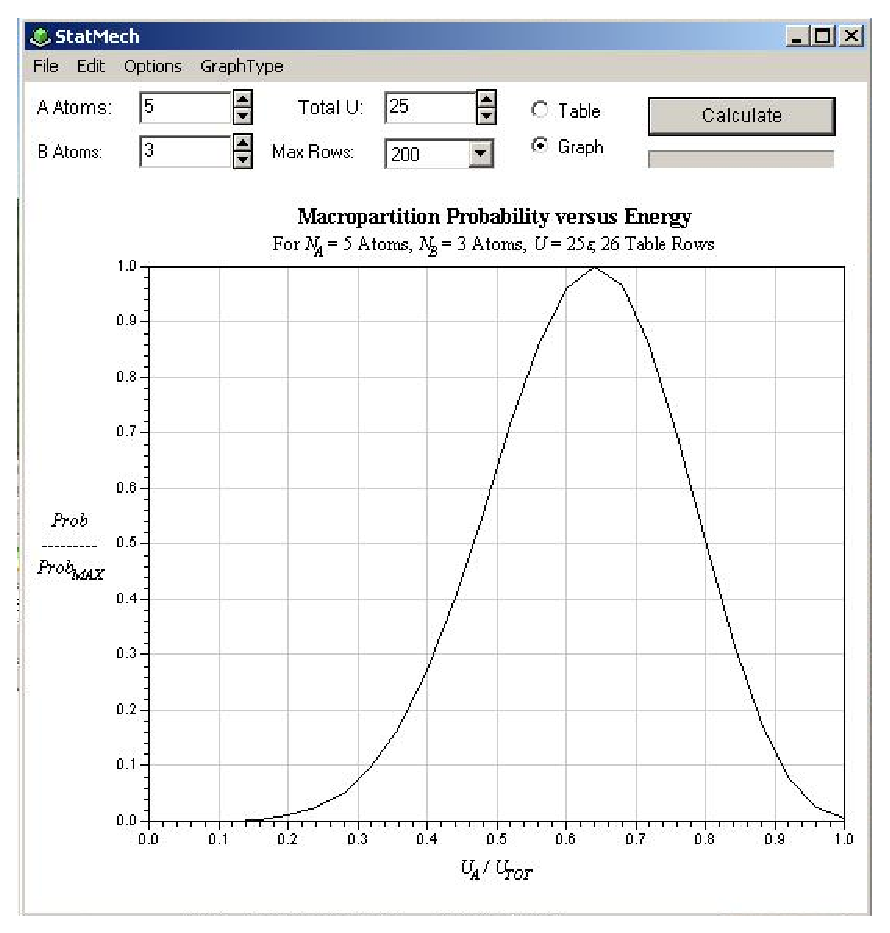
\includegraphics[height=4.0in]{einstein_solid/statmech2.eps}
\caption{The {\tt StatMech} window showing a graph of the multiplicities as a function
of $E_A/E_{int}$ where $E_A = q_A \hbar \omega$ and 
$E_{int} = q_{AB} \hbar \omega = (q_A+q_B)\hbar \omega$.}
\index{color page}
\end{center}
\end{figure}
The vertical axis is the probability of a particular macrostate divided by the maximum
probability of any macrostate.
The horizontal axis is  $U_A/U_{TOT}$ where 
$U_A$ is the energy of solid $A$ in units of $\epsilon$ (equivalent to $q_A$) and $U_{TOT}$ is the total
internal energy of the solid in units of $\epsilon$ (equivalent 
to the total number of quanta $q_{AB}$).
What is the value of $U_A/U_{TOT}$ for the most probable state?
How is this value related to the value of $q_A$ for the most probable macrostate? 
Also, explain in words what this plot is showing you.
\vspace{25mm}

(c) How wide is the distribution of microstates?
Measure this number by estimating the full-width-half-maximum (FWHM) from your graph.
Do this by finding the largest value on the vertical axis, divide that value by two, and find
the two points on either side of the peak where the distribution is equal to that
half-maximum.
Take the difference between these two points along the horizontal and this is the FWHM.
Record your result here.
%$U_A/U_{TOT} = 0.32
% sigma = 0.39-0.26 = 0.13
\answerspace{20mm}

(d) Now repeat steps 4.b-c with $U=100,000$ and $N_A$ and $N_B$ at their last values.
What is the most probable value of $U_A/U_{TOT}$ and the FWHM?
How have things changed?
%$E_A/U_{TOT} = 0.32
% sigma = 0.39-0.26 = 0.13
\answerspace{25mm}

\pagebreak[3]
(e) Keeping $U=100,000$ now repeat steps 4.b-c, but this time double the values of $N_A$ and $N_B$.
Record the most probable macrostate and the FWHM.
Repeat this doubling of the number of atoms in each solid while keeping $U$ fixed at least 3-4 times.
Record the most probable macrostate and the FWHM each time along with $N_A$ and $N_B$.
% 10:20 peak=0.32 sigma=0.13
% 20:40 peak=0.32 sigma=0.38-0.29=0.09
% 40:80 peak=0.32 sigma=0.36-0.30=0.06
% 80:160 peak=0.32 sigma=0.35-0.31=0.04
% 160:320 peak=0.32 sigma=0.34-0.32=0.02
\vspace{45mm}

(f) How does the value of $q_A$ for the most probable macrostate change as the number
of atoms increases?
\vspace{15mm}

(g) How does the FWHM change as the number of atoms increases?
\vspace{15mm}

\textbf{Activity 5: Irreversibility}

You will now use the results from the previous Activity to delve into some of the
implications of the statistical mechanics of the Einstein solid.

(a) As the number of atoms increases, what happens to the probability for finding the
system in a macrostate different from the most probable one?
Use the results of your calculations to explain your answer.
\vspace{15mm}

(b) When the system is in a macrostate far from the most probable one, what is the most
likely thing to happen as energy or heat flows around the system?
\vspace{15mm}

(c) For the last calculation in Activity 4 
what is the probability of the state with the minimum value of $q_A$?
%10^-813
In other words what is the probability that all of the quanta would end up all in solid $B$?
What is the probability of the most probable macrostate?
%qA=334, frac = 0.03186
\vspace{15mm}

(d) Go back to the questions in Activity 1 and look at your answers. 
Do they still appear to be correct?
A situation where all of the gas particles end up in one part of the container is a macrostate
of the system analogous
to the situation in Activity 5.c where all of the quanta end up in one  of the solids and 
not the other.
Answer those questions in Activity 1 again in terms of microstates, macrostates, and probability.

The behavior you are seeing here is for an Einstein solid, but is actually typical for
most macroscopic systems. These systems have a large number of atoms or molecules
with a variety of different energy states available.
They evolve to the most probable macrostate and there is essentially no chance to occupy a state
far from the most probable one. 
When two materials are first put in thermal contact they may be far from the most probable 
macrostate, but they equilibrate at that most probable one (where the temperatures are equal)
and never go back.
This is irreversibility.

%\vspace{15mm}


\bigskip

\textbf{Activity 6: Homework Problems} (E - exercise, P - problem)

\begin{enumerate}

\item(E) Consider the following `gas'.
It consists of four atoms in a cubical box. At any instant, there is a 50\% chance
of each atom being in the left half of the box ($L$) or the right half ($R$).
Make a table showing all the microstates of this system. (Hint: There are 16.)
How many macrostates are there?
How many microstates are in each macrostate?

\item (E) Show that for $N$ gas atoms in a box, the number of possible microstates is
$2^N$ when microstates are defined by whether a given molecule is in the left half
of the box or the right half of the box.
The volumes of each half are equal.


\item (E) Imagine that we have an ideal gas consisting of 15 molecules.  
We can flip the signs of each of the three velocity components of a given molecule w
without changing its overall energy (and thus without changing the gas's macrostate).  
How many possible patterns of sign choices are there?

\item (E) Calculate the multiplicity of an Einstein solid with $N = 1$ and $E_{int} = 6\epsilon$ 
by directly listing and counting the microstates.  
Check your work by using equation 3.

\item (E) Calculate the multiplicity of an Einstein solid with $N = 1$ and 
$E_{int} = 5\epsilon$  by directly listing and counting the microstates.  
Check your work by using equation 3.

\item (E) Use equation 3 to calculate the multiplicity of an 
Einstein solid with $N = 4$ and $E_{int} = 10\epsilon$.

\item (E) Use equation 3 to calculate the multiplicity of an 
Einstein solid with $N = 3$ and $E_{int} = 15\epsilon$.

\item (E) How many times more likely is that the combined system of 
solids described in the table below will be found in macropartition 3:3 than 
in macropartition 0:6, if the fundamental assumption is true?

\item (E) How many times more likely is it that the combined system of 
solids describe in the table below will not be found in macropartition 3:3 
than it is to be found in macropartition 0:6, if the fundamental assumption is true?

\begin{table}[hbt!]
\begin{center}
\begin{tabular}{|lccccc|} \hline
\hi Macropartition  & $E_A$ & $E_B$ & $\Omega_A$ & $\Omega_B$ & $\Omega_{AB}$ \\[5pt] \hline
\hi 0:6             & 0     & 6     & 1          & 28         & 28            \\[5pt]
\hi 1:5             & 1     & 5     & 3          & 21         & 63            \\[5pt]
\hi 2:4             & 2     & 4     & 6          & 15         & 90            \\[5pt]
\hi 3:3             & 3     & 3     & 10         & 10         & 100            \\[5pt]
\hi 4:2             & 4     & 2     & 15         & 6          & 90           \\[5pt]
\hi 5:1             & 5     & 1     & 21         & 3          & 63            \\[5pt]
\hi 6:0             & 6     & 9     & 28         & 1          & 28           \\[5pt] \hline
\hi                 &       &       &            & Total=     & 462         \\[5pt] \hline
\end{tabular}
\end{center}
\caption{Possible macropartitions for $N_A=1$, $N_B=1$, $E_{int}=6\epsilon$.}
\end{table}

\item (E) Consider the system consisting of a pair of Einstein solids in thermal contact.  
A certain macropartition has a multiplicity of $3.7 \times 10^{1024}$, while the total number of 
microstates available to the system in all macropartitions is $5.9 \times 10^{1042}$.  If we look 
at the system at a given instant of time, what is the probability that we will find it 
to be in our certain macropartition?

\item (E) Consider the system consisting of a pair of Einstein solids in thermal contact.  
A certain macropartition has a multiplicity of $1.2\times 10^{346}$, while the total number of 
microstates available to the system in all macropartitions is $5.9 \times 10^{362}$.  If we look 
at the system at a given instant of time, what is the probability that we will find it 
to be in our certain macropartition?

\item (E) Consider the system consisting of a pair of Einstein solids in thermal contact.  
Imagine that it is initially in a macropartition that has a multiplicity of $8.8 \times 10^{123}$.  
The adjacent macrostate closer to the equilibrium macrostate has a multiplicity
of $4.2 \times 10^{1234}$.  If we look at the system a 
short later, how many times more likely is it to have moved to the second macropartition 
than to have stayed with the first?

\item (E) Consider the system consisting of a pair of Einstein solids in thermal contact.  
Imagine that it is initially in a macropartition that has a multiplicity of $7.6 \times 10^{3235}$.  
The adjacent macropartition closer to the equilibrium macropartition has a multiplicity 
of $4.1 \times 10^{3278}$.  If we look at the system a short time later, how many times more likely 
is it to have moved to the second macropartition than to have stayed with the first?

\item(P) Suppose you put 100 pennies in a cup, shake it up, and toss them all into the
air.
(a) After landing, how many different head-tail arrangements (microstates) are possible for
the hundred pennies?
(b) What is the probability of finding exactly 50 heads? 
(c) 49 heads?
(d) 1 head?

\item(P) You ask your roommate to clean up a mess he or she made in your room.  Your roommate 
refuses, because cleaning up the mess would violate the second law of thermodynamics, and 
campus security's record of your roommate's legal violation is already excessive.  
Gently but firmly explain why complying will not put your roommate at risk of such an infraction.

\item(P) The classic statement of Murphy's law reads, `If something can go wrong, it will.'   
Explain how this is really a consequence of the second law of thermodynamics.  (Hint:  
What is the entropy of `wrong' in a given context compared to the entropy of `right'?)

\item(P) Run the {\it StatMech} program to answer the questions below.

\begin{enumerate}

\item For two Einstein solids in contact with 
$N_A = N_B = 100$ and 
$E_{int} = 200\epsilon$ answer the following questions.  (1) How many times more likely is the system 
to be found in the center macropartition than in the extreme macropartition where $E_A = 0$ 
and $E_B = 200\epsilon$ 
(2) What is the range of values that $E_A$ is likely to have more than 99.98\% 
of the time?  (3) if $E_A$ were initially to have the extreme value 0, how many times more 
likely is it to move to the next macropartition nearer the center than to remain in the 
extreme one?
\item  Answer the same question as in (a) for a run where you scale everything up by a 
factor of 10, so that $N_A = N_B = 1000$ and $E_{int} = 2000\epsilon$.
\item  Answer the same question as in (a) for a run where $N_A = N_B = 1000$ and 
$E_{int} = 200\epsilon$.  
Comment on the effect that increasing just the size of the system by a factor of 10 
has on these answers.
\item Answer the same question as in (a) for a run where $N_A = N_B = 100$ and $E_{int} = 2000\epsilon$.  
Comment on the effect that increasing just the energy available to the system by a factor 
of 10 has on these answers.

\end{enumerate}

\item(P) Consider two Einstein solids in thermal contact.  The solids have different 
values of N but are identical in all other respects.  It is plausible, since every atom 
in the combined system is identical, that in equilibrium the energy will be distributed 
among the solids in such a way that the average energy per atom is the same.  Use {\it StatMech} 
to test this hypothesis in the situation where $E_{int} = 1000\epsilon$ and $N_A$ and $N_B$ have various 
different values such that $N_A + N_B = 1000$.  (Set {\tt Max Rows} to 1000 so that you can see 
every macropartition).
\begin{enumerate}
\item Is it true in most cases that in the most probable macropartition the solids have 
energies such that the average energy per atom in each is the same?  Is it strictly 
true in every case?  Answer these questions by discussing the values $N_A$ and $N_B$ you tested, 
and whether the actual most probable macropartition is the same as that predicted by the hypothesis.
\item In any case where the hypothesis does not work, does increasing both $N_A$ and $N_B$ by a 
factor of 10 or 100 (but leaving $U$ alone) yield a result more or less consistent with 
the hypothesis?
\item Speculate as to the value of this hypothesis in the large-$N$ limit.
\end{enumerate}
\item(P) For the following questions, you will find that using {\it StatMech} is 
by far the fastest way to calculate the multiplicity.
\begin{enumerate}
\item  What is the entropy of an Einstein solid with 5 atoms and an energy of 
$15\epsilon$?  Express your answer as a multiple of $k_b$.
\item  What is the entropy of an Einstein solid with 50 atoms and an energy of $100\epsilon$?  
Express your answer as a multiple of $k_b$.
\end{enumerate}

\item(P) A certain macropartition of two Einstein solids has an entropy of $305.2k_b$.  
The next macropartition closer to the most probable one has an entropy of $335.5k_b$.  
If the system is initially in the first macropartition and we check it again later, 
how many times more likely is it to have moved to the other than to have stayed in the first?

\item(P) My calculator cannot display $e^x$ for $x> 230$.  One can calculate $e^x$ for larger 
values of $x$ as follows.  Define $y$ such that $x = y \ln 10$.  This means that 
$e^x = e^{y\ln 10} = (e^{\ln10})^y = 10^y = 10^{x\ln 10}$.  
Note that we can calculate 10 raised to a 
non-integer power (for example, 103.46) as follows:  
$10^{3.46} = 10^{3+0.46} = 10^3(10^{0.46}) = 2.9 \times 10^3$.  
Use these techniques to solve the following problem.  The entropy of the most probably 
macropartition for a certain system of Einstein solids is $6025.3k_b$, while the entropy 
of an extreme macropartition is only $5755.4k_b$.  What is the probability of finding the 
system at a given time in the extreme macropartition compared to that of finding it in 
the most probable macropartition?

\item(P) In principle, the entropy of a isolated system decreases a little bit whenever 
random processes cause its macropartition to fluctuate away from the most probable 
macropartition.  We can certainly see this with small systems. 
But is this really a possibility for a typical macroscopic system?  Imagine that 
we can measure the entropy of a system of two solids to within 2 parts in 1 billion.  
This means that we could just barely distinguish a system that has an entropy of 
4.99999999 J/K (eight 9s!) from one that has 5.00000000 J/K.  (This is a reasonable 
entropy for a macroscopic system).
\begin{enumerate}
\item Imagine that the entropy of the equilibrium macropartition is 5.00000000 J/K.  
Show that the approximate probability that at any given time later we will find the 
system in a macropartition with entropy 4.99999999 J/K ({\it i.e.}, with an entropy that 
is only barely measurably smaller) is about 10315,000,000,000,000 times smaller that 
the probability we will still find it to have entropy 5.00000000 J/K. (Hint:  See problem 17.)
\item Defend the statement that the entropy of an isolated system in thermal equilibrium 
never decreases.
\end{enumerate}

\end{enumerate}





\section{Entropy and Temperature}

\makelabheader %(Space for student name, etc., defined in master.tex)

\textbf{Objective}

To explore the connection between the fundamental definition of entropy and
temperature.

\textbf{Overview}

Consider the microscopic  definition of the entropy of a system
\begin{equation}
S = k_B \ln \Omega
\end{equation}
where $k_B$ is Boltzmann's constant and $\Omega$ is the multiplicity or number of 
microstates.
A microstate is defined by a particular arrangement of energy quanta among the
atoms.
A macrostate is defined by the total number of energy quanta $q$ and the number of atoms $N$.
We are building a model of an elemental solid ({\it e.g.}, like aluminum)
where
the total internal energy in the solid $E_{int}$ is described by
\begin{equation}
E_{int} = q \hbar \omega 
\end{equation}
where $\hbar$ is Planck's constant divided by $2\pi$ and $\omega$ is a constant that
characterizes the strength of the bonds between the atoms.
The parameter 
$q$ is the total number of quanta in the system and is a constant.
These quanta are statistically distributed over the $N$ atoms of the solid so
all possible states of the system are equally likely and the multiplicity $\Omega$
is
\begin{equation}
\Omega = \frac{(q+3N-1)!}{q!(3N-1)!} \qquad .
\end{equation}
This model of an elemental solid is called an Einstein solid.

We want to find a connection between the entropy defined in Equation 1 and the
temperature.
Recall how temperature is usually defined
relative to some properties of matter like the freezing and 
boiling points of water.
You are developing the microscopic picture of entropy, but it won't be successful until
you can connect it to the observed behavior of bulk matter and our familiar notions of 
temperature.

\textbf{Activity 1: The Entropy of Einstein Solids in Thermal Equilibrium}

(a) To start connecting the entropy to the temperature you have to study the 
behavior of the entropy as the energy changes.
To do this we will study two Einstein solids ($A$ and $B$) in thermal equilibrium with 
each other.
Their total internal energy will be
\begin{equation}
E_{int} = q_{AB}\hbar \omega = (q_A + q_B) \hbar \omega
\end{equation}
where $q_A$ and $q_B$ are the numbers of energy quanta in each solid and $q_{AB}$ is 
their sum.

Use the program {\it StatMech} (see the {\tt Physics Applications} menu)
for the configuration where you choose $N_A > 100$, $N_B > 80$ and $U>400$.
The label $U$ in the {\it StatMech} window refers to the total number of energy quanta 
in the system
in units of $\hbar \omega$ and is equivalent to $q_{AB}$ here.
An example of the output of {\it StatMech} is shown in Figure 1.
\begin{figure}[ht!]
\begin{center}
\includegraphics[height=4.0in]{entropy_temperature/statmech1.eps}
\caption{The {\tt StatMech} window showing the table of multiplicities for each microstate.
\index{color page}
Each row corresponds to a different value of $q_A$.}
\end{center}
\end{figure}
The first two columns in the lower panel of Figure 1 represent $U(A)$ and $U(B)$, 
the energies in each 
individual solid (again in units of $\hbar \omega$) and are equivalent to $q_A$ and $q_B$.
After you perform the calculation with {\it StatMech} scan quickly down the column
labeled `Omega(AB)'.
If any of the exponents you see exceed the value 307, then run the calculation again with 
smaller inputs until no exponent exceeds 307.
This limitation is a restriction on MicroSoft {\it Excel} that you will use later to make
plots.
Record your values of $N_A$, $N_B$, and $U$.
\vspace{15mm}

(b) Now generate plots of $S_{AB}=S_A + S_B$, $S_A$, and $S_B$ from the {\it StatMech} table.
You can do this with {\it Excel}, but there are some intermediate steps necessary.
Start Microsoft {\it Word} first.
Next, go to the {\it StatMech} window, highlight the table, copy it
 (see the {\tt Edit} menu on the {\it StatMech} window), and paste it into the {\it Word}
document. 
In {\it Word} edit out all the commas (`,') and asterisks (`*') in the file 
(use the {\tt Replace}
option under the {\tt Edit} menu).
Save the Word file, but save it as a plain text (`\*.txt') file.
You can now open the file in {\it Excel}.
When you open the file, {\it Excel} pops up a {\tt Text Import Wizard} 
that will guide you through
the format of the input file.
The defaults usually seem to work.
Use {\it Excel} to calculate and plot on one graph $S_{AB}$, $S_A$, and $S_B$
as a function of $q_A$.
Print out your plot and attach it to this unit.

(c) What is $q_A$ for the most probable macrostate? What mathematical condition can you impose
on the total entropy $S_{AB}$ to determine the most probable macrostate?
How do you think the temperatures of solids $A$ and $B$ are related at the most probable 
microstate?
\vspace{15mm}

(d) How are the slopes of $S_A$ and $S_B$ related to one another at the most probable
macrostate?
\vspace{30mm}

\newpage

(e) How is $E_A$, the energy in solid $A$ related to $q_A$?
How is $E_B$, the energy in solid $B$ related to $q_A$?
Remember that $q_{AB}$ is a constant and $q_{AB} = q_A + q_B$.
Calculate the differentials $dE_A$ and $dE_B$ and rewrite the answer in part 1.d
in terms of $dS_A/dE_A$ and $dS_B/dE_B$.
\vspace{45mm}

\textbf{Activity 2: Relating Entropy and Temperature}

(a) Using the spreadsheet you generated in Activity 1, calculate $dS_A/dq_A$ as a function
of $q_A$ and plot it. You can do this to an adequate approximation
by doing taking the difference between $S_A$ at adjacent values/rows
of $q_A$.
To do this suppose your spreadsheet has the values of $S_A$ in column $H$.
The {\it Excel} syntax for estimating the derivative for the first value of
$q_A$ (the first row) is 
`{\tt =(H2-H1)/1.0}' where {\tt H2} is the value in the second row and {\tt H1} is the
value in the first row.
The numerator of one is redundant, but it shows you are approximating the derivative
using the data from points that differ by 1.0 in $q_A$, the number of quanta in solid $A$.
The syntax for $dS_A/dq_A$ for the second value of $q_A$ is `{\tt =(H3-H2)/1.0}' and so on.
Do the same for $dS_B/dq_A$ and $dS_{AB}/dq_A$.
Does the slope of $S_{AB}$ pass through zero at the correct spot (recall part 1.c)?
How are $dS_A/dq_A$ and $dS_B/dq_A$ related at the most probable macrostate.
Does you plot agree with that result?
\vspace{15mm}

(b) If the energy $E_A$ and $q_A$ of solid $A$ increases what should the temperature 
of solid $A$ do?
If the energy $E_A$ of solid $A$ increases what happens to $dS_A/dq_A$ in your plot?
Do the temperature and $dS_A/dq_A$ change in the same  way or in a different way 
as $E_A$ increases?
\vspace{15mm}

(c) We want to come up with a relationship between temperature and the entropy.
From the results above (parts 1.a-e) you should have found
\begin{equation}
\frac{dS_A}{dE_A} = \frac{dS_B}{dE_B}
\end{equation}
and
\begin{equation}
T_A = T_B
\end{equation}
for the most probable macrostate.
This means there is some function of the temperature $T$ such that
\begin{equation}
f(T) = \frac{dS}{dE}
\end{equation}
for each solid that will be equal at equilibrium.
We want $f(T)$ to behave like the temperatures we are accustomed to using.
In other words, as the energy in the solid increases $T$ should increase.
Recall part 2.b and the behavior of $dS/dE$ as $T$ increases.
Try to guess a mathematical form of $f(T)$ that acts like `normal' temperatures
and one that doesn't. Explain your reasoning.
\vspace{30mm}

(d) How would you choose which of the forms you guessed in part 2.c is the correct one?
\vspace{15mm}

\textbf{Activity 3: Determining $f(T)$ and the Heat Capacity}

In the previous Activity you should have found that the mathematical form of $f(T)$
has to be something like $1/T^n$ where $n$ is some positive number.
This is necessary because your graphs should show that as the energy $E_A$ (and the number
of quanta $q_A$) of the solid 
increases $f(T)=dS/dE$ goes down. To make sure the temperature $T$ behaves reasonable
(and goes up with $E_A$ and $q_A$) $f(T)$ must be some inverse of function of $T$.
To decide exactly which function is right requires comparing Equation 7 or some
result from it to some data.

Recall the table of heat capacities we generated in the laboratory entitled
{\it Calorimetry}.
Use those results to fill in Table 1 making sure that you are using molar 
heat capacities.
\begin{table}
\begin{center}
\begin{tabular}{|p{0.8in}|l|p{0.8in}|l|} \hline
\hi Solid    & $dE/dT$ per mole & Solid      & $dE/dT$ per mole   \\[2pt] \hline
\hi          &                  &            &       \\[2pt] \hline
\hi          &                  &            &      \\[2pt] \hline
\hi          &                  &            &      \\[2pt] \hline
\end{tabular}
\caption{Molar specific heats ($(1/n)dE/dT$) for several elemental solids.}
\end{center}
\end{table}
%Consider Table 1 of heat capacities ($dE/dT$) for several elemental solids
%for high temperatures.
%\begin{table}
%\begin{center}
%\begin{tabular}{|p{0.8in}|l|p{0.8in}|l|} \hline
%\hi Solid    & $dE/dT$ per mole & Solid      & $dE/dT$ per mole   \\[2pt] \hline
%\hi Lead     & $26.4~J/K-mole$    & Gold     & $25.4~J/K-mole$      \\[2pt]
%\hi Silver   & $25.4~J/K-mole$    & Copper   & $24.5~J/K-mole$      \\[2pt]
%\hi Iron     & $25.0~J/K-mole$    & Aluminum & $26.4~J/K-mole$      \\[2pt] \hline
%\end{tabular}
%\caption{Heat capacities ($dE/dT$) for several elemental solids.}
%\end{center}
%\end{table}
 The heat capacities are constant with respect to temperature and are similar in value to
one another.
These are the data that will help us determine $f(T)$.
To calculate $dE/dT$ we must find a relationship between $E$ and $T$ for the Einstein solid.

(a) Start with Equations 1 and 7 and the chain rule and show the following.
\begin{equation}
\frac{dS}{dE} = k_B \frac{1}{\Omega} \frac{d\Omega}{dE}
\end{equation}
\vspace{15mm}

(b) Use Equation 2 to show 
\begin{equation}
dE = \hbar \omega dq \qquad {\rm and} \qquad  
    \frac{d\Omega}{dE}=\frac{1}{\hbar\omega} \frac{d\Omega}{dq}
\qquad .
\end{equation}
\vspace{15mm}

\newpage

(c) Starting with Equations 1 and 3 one can show
\begin{equation}
\frac{d\Omega}{dq} = \frac{3N\hbar \omega}{E} \Omega
\qquad .
\end{equation}
Combine this equation (number 10) and the  results from 3.a-b to 
get a relationship for $dS/dE$ for the Einstein solid in terms
of $N$ and $E$.
Set that expression equal to $f(T)$,
and solve for $E$ the internal energy.
It is the derivative of this last equation ($(1/n)dE/dT$) that will give you the molar specific heat.
What function of $f(T)$ will give a result that is independent of temperature when you
take the derivative with respect to $T$ of your expression for the internal energy $E$?
\vspace{45mm}

(d)  What is the final form of Equation 7 and $f(T)$?
\vspace{15mm}

(e) Determine the mean and standard deviation of the heat capacity of the elemental solids in
Table 1.
Calculate the molar specific heat ($(1/n)dE/dT$) for the Einstein solid using your results from
parts 3.c-d.
Is the molar specific heat for the model of the Einstein solid consistent with the measured ones?
\vspace{45mm}


\textbf{Activity 4: The Second Law of Thermodynamics}

(a) Go back to your plots of the entropy as a function of $q_A$ from part 1.b. 
Consider two Einstein solids that are brought together at a value of $q_A$ that is higher
than the equilibrium one at the most probable macrostate.
Choose a value of $q_A$ that is halfway between the most probable value and the maximum.
Once the two Einstein solids are in contact, how will the system evolve?
What happens to $S_A$ and $S_B$? Do they go up, down, or stay the same?
What happens to the total entropy $S_{AB}$?
In fact, based on your plot from part 2.b, is there any circumstance where
$S_{AB}$ will not increase?
\vspace{30mm}

(c) To  vividly see what happens when Einstein solids come in thermal contact,
run the program {\it equilib.exe} available in the {\tt Physics Applications} menu.
This program starts with two Einstein solids with all the energy quanta in solid $B$.
It simulates the evolution of the two solids as they march toward
thermal equilibrium.
Click {\tt Evolve} to see the simulation run.

What you should have discovered in the previous part is that the entropy of the combined systems
always increases regardless of what configuration the Einstein solids are in when they
come in contact.
The system always evolves to the most probable, most disordered
 macrostate where the temperatures will
be equal and the entropy is a maximum.
The energy quanta are most spread out.
This result is stated in several different ways, but the most succinct is simply
$\Delta S > 0$ for an isolated system.
The entropy of an isolated system always increases.
This is called the Second Law of Thermodynamics.

\bigskip

\textbf{Activity 4: Homework Problems}

\begin{enumerate}
 
\item (E) An object's entropy is measured to increase by $0.1~ J/K$ 
when we add $35~ J$ of energy.  What is its approximate temperature?  
(Assume that the object's temperature does not change much when we add the $35~J$.)

\item (E) A certain Einstein solid's entropy changes from 
$305.2k_b$ to $338.1k_b$ when we add 1 unit $\epsilon$ of energy.  
What is the value (and units) of $k_bT/\epsilon$ for this solid?  
If $\epsilon = 1.0~eV$, what is its temperature $T$?

\item (E) Does it make sense to talk about the 
temperature of a vacuum?  If so, how could you measure or calculate it?  
If not, why not?  

\item (E) An Einstein solid in a certain macrostate has a multiplicity of $3.8 \times 10^{280}$.  
What is its entropy (expressed as a multiple of $k_B$)?

\item (E) A pair of Einstein solids in a certain macropartition has multiplicities of 
$4.2 \times 10^{320}$ and $8.6 \times 10^{132}$.  What are the entropies of 
each solid?  What is the total 
entropy of the system in this macropartition?  (Express entropies as multiples of $k_b$.)

\item (E) Is it really true that the entropy of an isolated system consisting of two 
Einstein solids never decreases?  (Consider a pair of very small solids.)  Why is this 
statement more accurate for large systems than for small systems?  Explain in your own words.

\item (P) In lab we argued on fairly fundamental grounds 
that $dS/dU = f(T)$.  In principle, we could define $f(T)$ to be anything 
that we like:  this would amount to defining temperature and its scale. 
Still, some definitions would violate deeply embedded preconceptions 
about the nature of temperature.  
For example, the simplest definition of temperature would be $dS/dU = T_{new}$.  
Show that this definition
\begin{enumerate}
\item Would imply that $T_{new}$ has units of $K^{-1}$ and
\item Would imply that heat would flow spontaneously from objects with 
low $T_{new}$ to objects with high $T_{new}$.  
This would imply that object with low values of $T_{new}$ are hot, while 
objects with high values $T_{new}$ are cold (we might want to call $T_{new}$ 
so defined {\it coolness} instead of {\it temperature}).  
While we could define temperature in this way, it would really fly 
in the face of convention (if not intuition).
\item If we did define coolness $T_{new}$ in this way, what ordinary 
temperature $T$ would an object with absolutely zero coolness (
$T_{new} = 0$) have?  What about something that is infinitely cool ($T_{new} = \infty$)?
\end{enumerate}

\item (P) Imagine that the entropy of a certain substance as a function of 
$N$ and $U$ is given by the formula $S = Nk_b \ln U$. Using the definition of temperature, 
show that the thermal energy of this substance is related to its temperature 
by the expression $U=Nk_b T$.

\item (P) Imagine that the multiplicity of a certain substance is 
given by $\Omega(U,N) = Ne^{\sqrt{NU/\epsilon}}$, where $\epsilon$ is some unit of energy.  
How would the energy of an object made out of this substance depend 
on its temperature?  Would this be a `normal' substance in our usual sense 
of temperature.

\item (P) Consider an Einstein solid having $N = 20$ atoms.  
\begin{enumerate}
\item What is the solids temperature when it has an energy of $10\epsilon$, 
assuming that $\epsilon =h\omega = 0.02 eV$?  Calculate this directly from the 
definition of temperature by finding $S$ at $10\epsilon$ and $11\epsilon$, computing 
$dS/dU \approx [S(11\epsilon) - S(10\epsilon)]/\epsilon$, and then applying 
the definition of temperature.  (You will find that your work will 
go faster if you use {\it StatMech} to tabulate the multiplicities.)
\item How does this compare with the result from the formula $U = 3Nk_bT$ 
(which is only accurate if $N$ is large and $U/3N\epsilon > 1$)?
\item If you have access to {\it StatMech}, repeat for 
$N = 200$ and $U =100\epsilon$.  
(Hint:  If your calculator cannot handle numbers in excess of $10^{100}$, 
use the fact that in $(a \times 10^b) = \ln a + b \ln 10 $).
\end{enumerate}

\item (P)  A newly-created material has a multiplicity
$$
\Omega = \alpha N E
$$
where $N$ is the number of atoms in the solid,
$E$ is the total, internal energy in the solid, and $\alpha$ is a constant of 
proportionality.
\begin{enumerate}
\item How does the temperature of the new material depend on the internal energy?
\item What is the molar heat capacity for this solid?
\item Could this material really exist? Why or why not?
\end{enumerate}

\item (P)  A newly-created material has a multiplicity
$$
\Omega = \beta M E^2
$$
where $N$ is the number of atoms in the solid,
$E$ is the total, internal energy in the solid, and $\alpha$ is a constant of 
proportionality.
\begin{enumerate}
\item How does the temperature of the new material depend on the internal energy?
\item What is the molar heat capacity for this solid?
\item Could this material really exist? Why or why not?
\end{enumerate}


\end{enumerate}




%
\section{The Interactions of Electric Charges\footnote{%
Adapted from A. Arons, \underbar{A Guide to Introductory Physics Teaching},
Wiley \& Sons, 1990; and R. Chabay and B. Sherwood, \underbar{Electric
\& Magnetic Interactions}, Wiley \& Sons, 1995.
}}

\makelabheader %(Space for student name, etc., defined in master.tex)

\textbf{Objectives}

\begin{itemize}
\item Note the number of different kinds of charge
\item Characterize the interactions between like and unlike charges
\item Discover the nature of electrical force
\end{itemize}
\textbf{Introduction}

You probably already know this, but electric force between charge
objects is proportional to the amount of charge on each of the objects,
acts along a line between the objects, and decreases rapidly as the
distance between the two objects increases. In the following activities,
you will find out if invisible tape exhibits these properties, and
thus whether such tape becomes electrically charged and therefore
useful in the study of electrical interactions. Use strips of tape
around 20 cm long. Shorter pieces are too inflexible; longer ones
too difficult to handle. Fold one end of each strip to make a non-stick
handle and stick a paper clip on this handle.

Note: The real world is messy. Straight-forward experimental manipulations
and accurate measurements are not always easy to come by. Try to keep
your frustration level down. Rough observations are good enough for
this lab.

\textbf{Apparatus}

\begin{itemize}
\item Invisible ({}``Scotch'') tape
\item Paper clips (2)
\end{itemize}
\textbf{Investigation 1: Your Hand and a U Tape}

\textbf{Preparing a U Tape:}

\begin{enumerate}
\item Stick a strip of tape, sticky-side down, onto the table top and smooth
it down with your thumb or fingers. This base tape provides a standard
work surface and thus ensures consistent results.
\item Stick a second strip of tape, sticky-side down, on top of the base
tape and smooth it down well with thumb or fingertips. Write the letter
U (for Upper) on the handle of this strip.
\item Holding the handle and with a very quick motion, pull the U tape up
and off the base tape, which should remain stuck to the table.
\end{enumerate}
\textbf{Activity:}

\begin{enumerate}
\item Hang the U tape vertically from the edge of the table, handle down.
\item Briefly describe what happens when you slowly bring your hand near
the hanging tape.\vspace{15mm}

\item Is the behavior different when you approach the other side of the
tape?\vspace{15mm}

\end{enumerate}
\textbf{Note:} Tape should react to the presence of your hand. If
not, repeat the U tape preparation.

\textbf{Prediction:} How would you expect two U tapes to interact:
repel each other, attract each other, or not affect each other? Briefly
explain your reasoning.
\vspace{1in}

\textbf{Investigation 2: Two U Tapes}

\textbf{Activity 1:}

\begin{enumerate}
\item Prepare a second U tape, remembering to mark U on its handle.
\item Doing your best to keep your hand out of the way (recall that your
hand attracts the tape--perhaps hold the second strip horizontally
in two hands), bring the second U tape near the hanging first one.
Describe what happens.\vspace{15mm}

\item Hand the second U tape beside the first.
\end{enumerate}
\textbf{Activity 2:}

\begin{enumerate}
\item Suspend a U tape from a piece of thread or hair.
\item Approach the suspended tape from various directions with the other
U tape. Do the tapes repel along or at an angle to the line between
the objects?
\end{enumerate}
\vspace{0.3cm}
{\centering 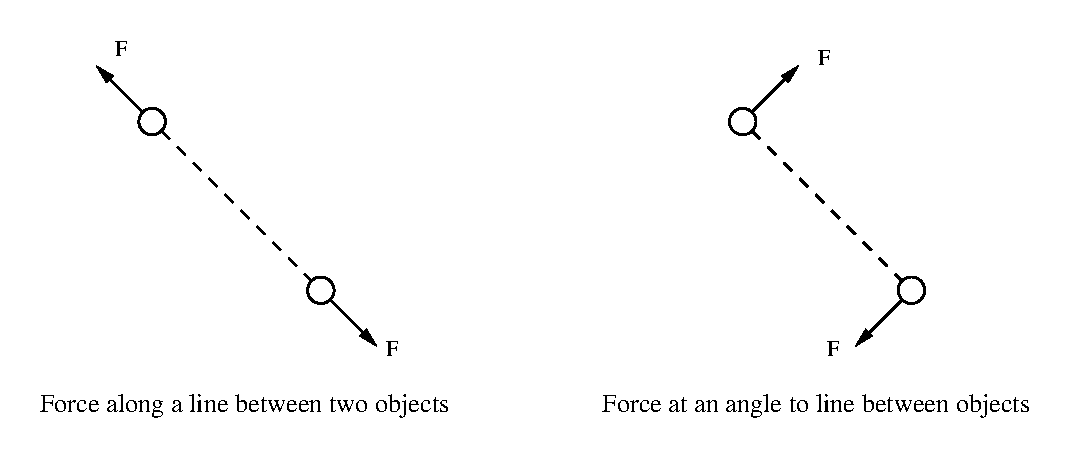
\includegraphics{interactions_of_electric_charges/int_elec_charges_fig_1.eps} \par}
\vspace{0.3cm}

\vspace{15mm}
\textbf{Note:} You may have noticed that if you handle a U tape too
much, it loses its interaction strength. Remember to reactivate the
strips regularly.

\textbf{Activity 3:}

\begin{enumerate}
\item Note that when you move one U tape slowly toward a hanging U tape,
there is a distance at which repulsion is first detectable.
\item Note what happens as you repeatedly halve the distance between the
strips.\vspace{15mm}

\item Graph--very roughly--the deflection of the hanging tape as a function
of the distance between tapes. Note that this deflection from an original
vertical position is a measure of the strength of the interaction.
\end{enumerate}
\vspace{0.3cm}
{\centering 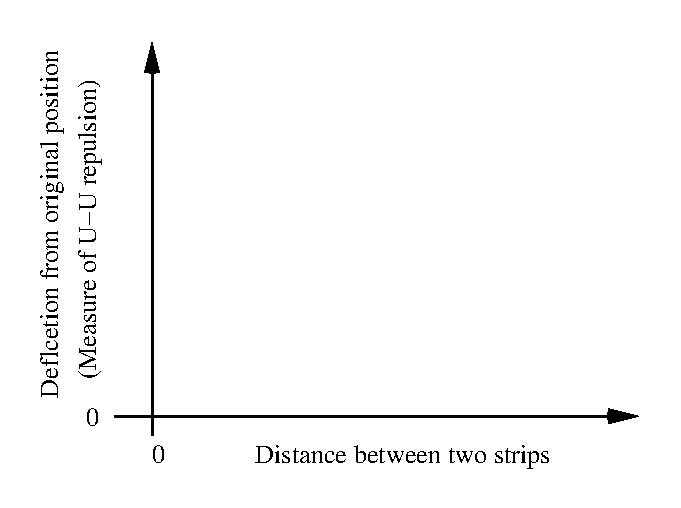
\includegraphics{interactions_of_electric_charges/int_elec_charges_fig_2.eps} \par}
\vspace{0.3cm}

\textbf{Activity 4:}

\begin{enumerate}
\item Hold the bottom of a hanging, active U tape and slowly rub your thumb
or fingers back and forth along its slick side.
\item Describe the changes in how this U tape interacts with your hand.
Also, with another U tape.\vspace{15mm}

\item Reactivate two U tapes. Hang one from the table and note how strongly
the other one repels it.\vspace{15mm}

\item Run a finger along the length of the hanging tape's slick side, but
touch only a portion of its width (not the full side). Be sure to
leave a continuous vertical section untouched. 
\item Do the two tapes now exhibit a weaker or stronger repulsion, or no
repulsion at all?\vspace{15mm}

\item Try to explain what has been going on in this activity.\vspace{15mm}

\end{enumerate}
\textbf{Questions:}

\begin{enumerate}
\item Are U tapes electrically charged?\vspace{10mm}

\item Do U tapes have like or unlike electric charge?\vspace{10mm}

\end{enumerate}
\textbf{Investigation 3: A U and an L Tape}

\textbf{Challenge:} How would you prepare a tape that might have an
electric charge unlike the charge on a U tape?

\textbf{Preparing an L Tape:}

\begin{enumerate}
\item Stick a strip of tape, sticky-side down, on top of the base tape and
smooth it down well with thumb or fingertips. Write the letter L (for
Lower) on the handle of this strip.
\item Stick a second strip of tape, sticky-side down, on top of the L tape
and smooth it down well with thumb or fingertips. Write the letter
U (for Upper) on the handle of this strip.
\item Lifting the handle of the L tape, slowly pull it along with the U
tape up and off the base tape, which should remain stuck to the table.
\item Hang the double layer of tape vertically from the edge of the table,
handles down. Check that there is no interaction between it and your
hand. If there is, do what you need to so the interaction no longer
occurs.
\item While holding down the handle of the L tape, quickly life off the
U tape, then hang it vertically from the edge of the table, not too
close to the L tape.
\end{enumerate}
\textbf{Prediction:} Will the L tape attract, repel, or not interact
with the U tape if the two are brought within proximity of one another?
\vspace{1in}

\textbf{Activity 1:}

\begin{enumerate}
\item With your hand, check that both the U tape and the L tape are active.
How can you tell?\vspace{15mm}

\item What interaction do you observe between an L tape and a U tape?\vspace{15mm}

\end{enumerate}
\textbf{Prediction:} Will an L tape attract, repel, or not interact
with another L tape if the two are brought within proximity of one
another?
\vspace{15mm}

\textbf{Activity 2:}

\begin{enumerate}
\item Make another pair of L and U tapes.
\item Be sure that all four tapes are active.
\item What interaction do you observe between two L tapes?\vspace{15mm}

\item Summarize the interactions you have observed between U and L tapes:
\end{enumerate}
\begin{quote}
L-U:

U-U:

L-L:
\end{quote}
~~~~5.~State a rule for the pattern of interactions between like
and unlike charges:
\vspace{20mm}

\textbf{Activity 3:}

\begin{enumerate}
\item Note that when you move an active L tape slowly toward a hanging U
tape, there is a distance at which attraction is first detectable.
\item Note what happens as you repeatedly halve the distance between the
strips.\vspace{15mm}

\item Graph--very roughly--the deflection of the hanging tape as a function
of the distance between tapes. Note that this deflection from an original
vertical position is a measure of the strength of the interaction.
\end{enumerate}
\vspace{0.3cm}
{\centering 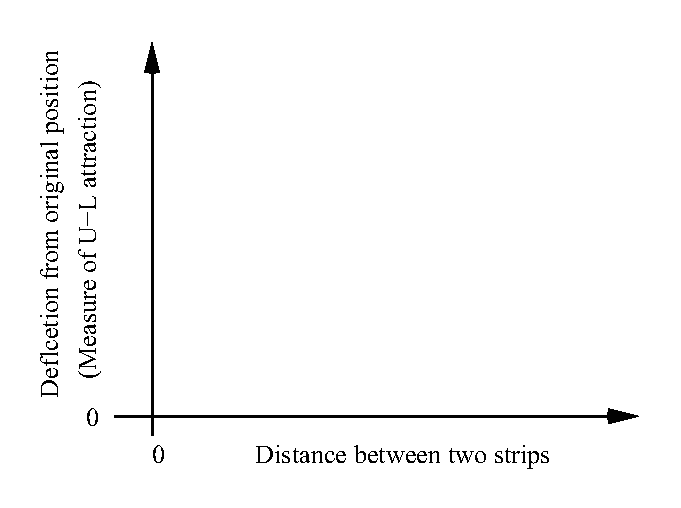
\includegraphics{interactions_of_electric_charges/int_elec_charges_fig_3.eps} \par}
\vspace{0.3cm}

\textbf{Questions:}

\begin{enumerate}
\item Why is this task more difficult now than it was with two U tapes?\vspace{15mm}

\item Do the forces between U and L tapes lie along or at an angle to the
line between the tapes?
\end{enumerate}
\begin{quotation}
Force by U tape on L tape:
\vspace{10mm}

Force by L tape on U tape:\vspace{10mm}

\end{quotation}
\textbf{Summary:} In the table below, state very briefly what you
observed.

\vspace{0.3cm}
{\centering \begin{tabular}{|l|l|}
\hline 
~~~~~~~~~~~~~~~~~~~~~~~~~~~~~~~~\textbf{Property}&
\textbf{Experimental Observation of U and L Tapes}\\
\hline
\hline 
There are two kinds of charges;&
U-U:\\
like charges repel;&
L-L:\\
unlike charges attract.&
U-L:\\
\hline 
Electric force is proportional to amount of charge.&
U tape and partially neutralized U tape:\\
&
\\
\hline 
Electric force acts along a line between charges.&
U-U:\\
&
U-L:\\
\hline 
The strength of interaction decreases&
U-U:\\
rapidly as distance between the charges increases.&
U-L:\\
\hline
\end{tabular}\par}
\vspace{0.3cm}

\textbf{Activity 4:}

\begin{enumerate}
\item Quickly lift off the base tape.
\item Is it U-like or L-like? How can you tell?\vspace{15mm}

\end{enumerate}
\textbf{Questions:}

\begin{enumerate}
\item How does all of this happen: How do the tapes become charged? Why
are both U and L tapes attracted to your hand? Why does rubbing the
slick side of a tape with your finger appear to neutralize the tape?\vspace{20mm}

\item What do you think charges are?\vspace{15mm}
\end{enumerate}



\section{Music to Our Ears: Standing Waves in Strings}

Name \rule{2.0in}{0.1pt}\hfill{}Section \rule{1.0in}{0.1pt}\hfill{}Date
\rule{1.0in}{0.1pt}

\textbf{Aim:}
\begin{itemize}
\item  to study the natural modes of vibration of a stretched string
\end{itemize}

\textbf{Equipment:}
\begin{itemize}
\item  string vibrator and power supply
\item  inelastic braided string
\item  2 clamps
\item  superpulley
\item  mounting rod for the superpulley
\item  mass and hanger set
\item  balance
\item  tape measure
\end{itemize}


How do we make musical sounds? To make a sound , we need something that vibrates. If we want to make musical notes you usually need the vibration to have an almost constant frequency: that means stable pitch. We also want a frequency that can be easily controlled by the player. In electronic instruments this is done with electric circuits or with clocks and memories. In non-electronic instruments, the stable, controlled vibration is produced by a standing wave. Here we discuss the way strings work. This is also a good introduction for studying wind instruments, because vibrating strings are easier to visualise than the vibration of the air in wind instruments, but the math is very similar.  

\textbf{Introduction}

Waves are oscillations in an elastic medium:

\begin{itemize}
\item  your own vocal cords (the medium) vibrating as air is forced over them by your lungs; 
\item  a stretched string (the medium) on a musical instrument vibrating as it is bowed, hammered or plucked; 
\item  pressure oscillations in a column of air (the medium) in a wind instrument, organ pipe or your own oral and nasal cavities.
\end{itemize}

In each case the medium has an equilibrium state, and when displaced or otherwise perturbed from that state, experiences a force which tends to restore it to equilibrium. For small perturbations, the restoring force is proportional to the displacement and the medium becomes a simple harmonic oscillator.

There are also waves that do not require a medium, namely electromagnetic waves, which will be discussed later in the course.

\textbf{Background}

Standing waves (stationary waves) are produced by the interference of two traveling waves, both of which have the
same wavelength, speed and amplitude, but travel in opposite directions through the same medium. The necessary conditions for the production of
standing waves can be met in the case of a stretched string by having waves set up by some vibrating body, reflected at the end of the string and then interfering with the oncoming waves.

One characteristic of every standing wave pattern is that there are points along the medium which appear to be standing still. These points, sometimes described as points of no displacement, are referred to as nodes. There are other points along the medium which undergo vibrations between a large positive and large negative displacement. These are the points which undergo the maximum displacement during each vibrational cycle of the standing wave. In a sense, these points are the opposite of nodes, and so they are called antinodes. A standing wave pattern always consists of an alternating pattern of nodes and antinodes. When a standing wave pattern is established in a medium, the nodes and the antinodes are always located at the same position along the medium; they are "standing still." It is this characteristic which has earned the name "standing wave."

A stretched string has many natural modes of vibration (three examples are shown below). If the string is fixed at both ends then there must be a node at each end. It may vibrate as a single segment, in which case the length ($L$) of the string is equal to 1/2 the wavelength ($\lambda $) of the wave. It may also vibrate in two segments with a node at each end and one node in the middle; then the wavelength is equal to the length of the string. It may also vibrate with a larger integer number of segments. In every case, the length of the string equals some integer number of half wavelengths.

\vspace{0.3cm}
\begin{center}
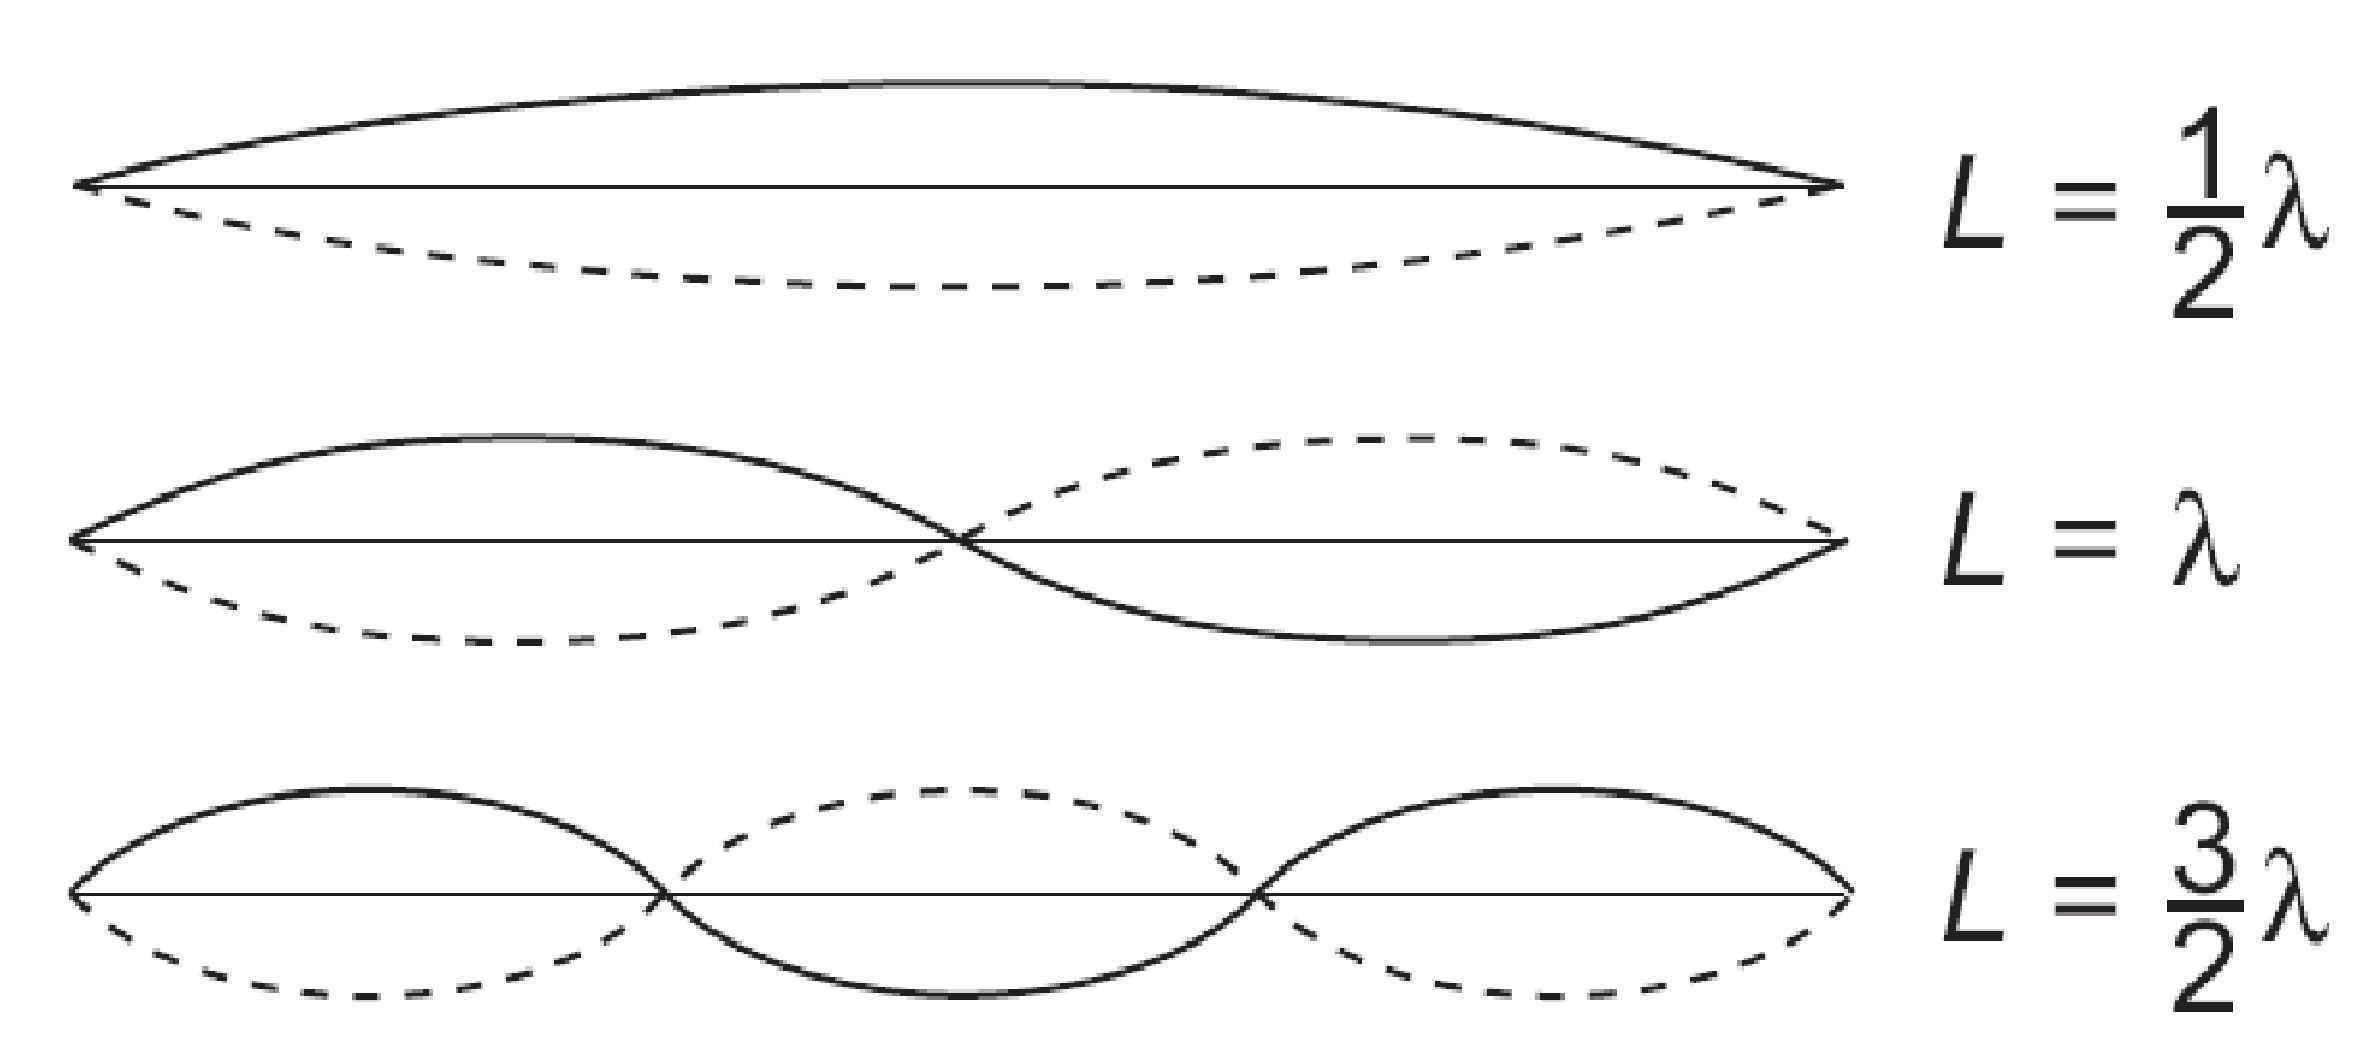
\includegraphics[width=3in]{Standing_waves_strings_fig1_tb.eps}
\end{center}
\vspace{0.3cm}

If you drive a stretched string at an arbitrary frequency, you will probably not see any particular mode; many modes will be mixed together. But, if the tension and the string's length are correctly adjusted to the frequency of the driving vibrator, one vibrational mode will occur at a much greater amplitude than the other modes.
For any wave with wavelength ($\lambda $) and frequency $f$, the speed, $v$, is:
\begin{equation}
v=\lambda f
\end{equation}

The speed of a wave on a string is also given by:
\begin{equation}
v=\sqrt{\frac {T}{\mu }}
\end{equation}
where $T$ is the tension in the string and $\mu $ is the linear density (mass/length) of the string.

In this experiment, standing waves are set up in a stretched string by the vibrations of an electrically-driven String Vibrator. The tension in the string equals the weight of the masses suspended over the pulley. You can alter the tension by
changing the masses. $L$ is the length of the string and $n$ is the number of segments. (Note that $n$ is not the number of nodes). Since a segment is 1/2 wavelength then


\begin{equation}
\lambda =\frac {2L}{n } \qquad n=1,2,3,...
\end{equation}



\vspace{0.3cm}
\begin{center}
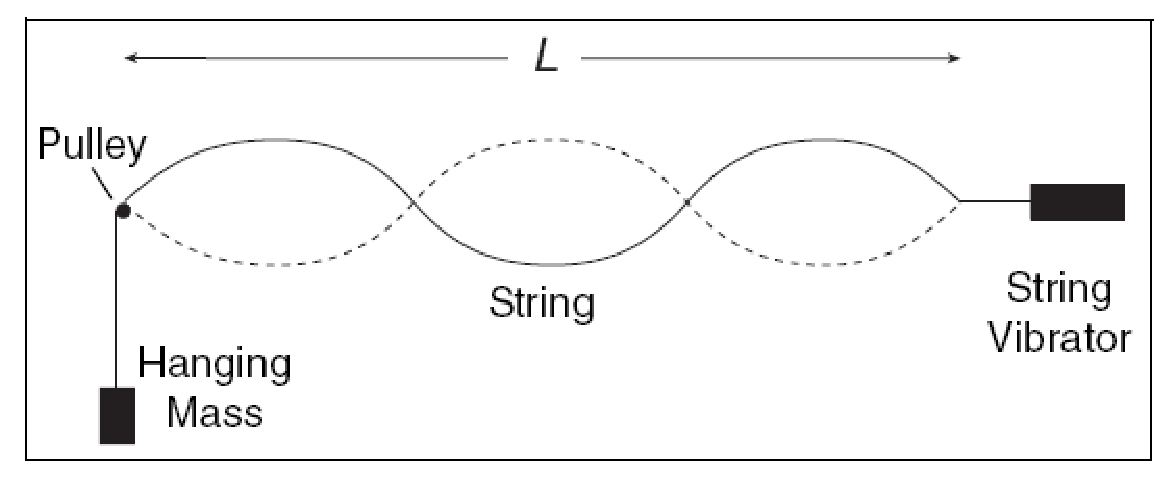
\includegraphics[width=250pt]{Standing_waves_strings_figure2.eps}
\end{center}
\vspace{0.3cm}


\textbf{Procedure}

\textbf{1. } Measure the exact length of a piece of string several meters long. Measure the mass of the
string and calculate the linear density (mass/length).(If your balance is not precise enough to measure that length of string, use a longer
piece of string to calculate the linear density.)

\vspace{2cm}

\textbf{2. } Clamp the String Vibrator and pulley about 100 cm apart. Attach the string to the vibrating blade, run it over the pulley, and hang about 200 g of mass from it. Cut off the excess string.

\textbf{3. } Measure from the knot where the string attaches to the String Vibrator to the top of the pulley.
This is the distance $L$. ($L$ is NOT the total length of the string that you measured in \textbf{1 }.) Record the value here: $L$ =

\vspace{0.3cm}
\begin{center}
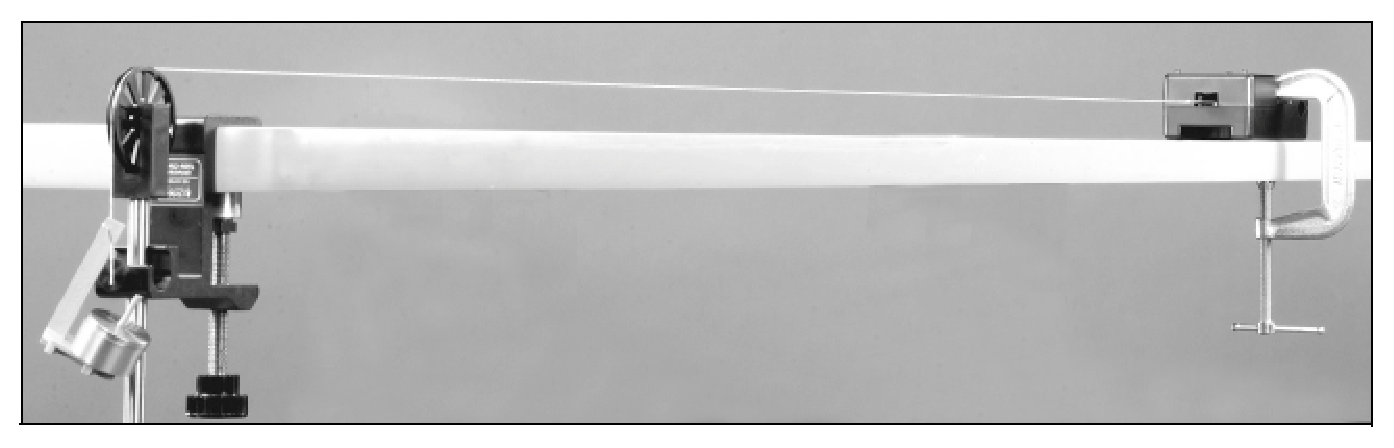
\includegraphics[width=320pt]{Standing_waves_strings_figure3.eps}
\end{center}
\vspace{0.3cm}

\textbf{4. } Connect the AC power supply to the String Vibrator.

\textbf{5. } Adjust the tension by adding to or subtracting from the hanging mass so that the string vibrates in 2 segments. Adjust the tension further to achieve a ``clean'' node at the center. Also check the end of the vibrating blade; the point where the string attaches should be a node. It is more important to have a good node at the blade than it is to have the largest amplitude possible. However, it is desirable to have the largest amplitude possible while keeping a good node.

\textbf{6. } Record the hanging mass, $m$. How much uncertainty is there in your value? By how much can you change the hanging mass before you see an effect? Record the uncertainty.

\vspace{3cm}

\textbf{Part A: Speed of the Wave }

\textbf{a. } Calculate the tension (including the uncertainty) in the string.

\vspace{3cm}

\newpage

\textbf{b. } Calculate the speed $v_A$ (including uncertainty) of the wave from your observed values of tension
($T$) and linear density ($\mu $). Record your calculated value with the uncertainty and the correct number of significant
figures.


\vspace{4cm}

\textbf{c. } Calculate the speed $v_B$ from the wavelength ($\lambda $) and frequency ($f$). (In the U.S. $f$ = 60.0 Hz.)

\vspace{4cm}

\textbf{d. } Compare the two values ($v_A$ and $v_B$) of speed. What is the difference? How does the difference compare
to the uncertainty that you determined in \textbf{b }?

\vspace{4cm}

\textbf{e. } Calculate the percentage by which $v_A$ deviates from $v_B$.

\begin{equation}
\% Deviation =\frac {v_A - v_B}{v_B} \times 100\%
\end{equation}

\vspace{3cm}

\newpage

\textbf{Part B: Linear Density}

\textbf{a. } Produce standing waves of 3, 4, 5, etc. segments in the string by reducing the hanging mass. Get as many as you can. Create a table here with the headings $n$ (number of segments), $m$ (mass), $T$ (tension in the string which is the same as $mg$), and $\frac{1}{n^2}$.

\vspace{6cm}

\textbf{b. } For every value of mass, calculate the tension in the string, and include in the above table.

\textbf{c. } In $Excel$, plot a graph of $T$ versus $n$ including a trend line with a polynomial fit of order 2, and attach it at the end of this activity. What is the power of $n$?
\vspace{20mm}

\textbf{d. } For every value of $n$, calculate $\frac{1}{n^2}$ and include in above table. In $Excel$, plot a graph of $T$ versus $\frac{1}{n^2}$. Does the graph look linear? If so, include a linear trend line. Print the graph and include with this unit.
\vspace{20mm}

\textbf{e. } Using the LINEST function in $Excel$ (see \textbf{Appendix C}), find the slope of the graph and its uncertainty. Record the values here (including units):

\vspace{20mm}

\textbf{f. } Combine the equations in the \textbf{Background } section, and show that the tension can be written as:

\begin{equation}
T=4\mu f^{2}L^{2}\frac{1}{n^2}
\end{equation}

\vspace{25mm}

Thus the slope of a $T$ versus $\frac{1}{n^2}$ graph is $4\mu f^{2}L^{2}$.

\textbf{g. } Use the slope from your graph to calculate the density, $\mu $, of the string. Also calculate the uncertainty in $\mu$, assuming the fractional uncertainty in $\mu$ is the same as the fractional uncertainty in the slope.

\vspace{5cm}

\textbf{h. } Compare this measured value of string density to the accepted value. (You calculated the accepted value of $\mu $ from the mass and length of the string at the beginning of the experiment). Does the accepted value fall within the uncertainty limits of your calculated value?

\vspace{50mm}

%\textbf{i. } Calculate the percent deviation of the measured value of $\mu $ from the accepted value.

%\begin{equation}
%\% Deviation =\frac{Measured-Accepted}{Accepted}\times 100\%
%\end{equation}

%\vspace{4cm}

\textbf{Further Investigation}

%\textbf{1. } Hang a mass on the string with a value that is about halfway between the masses that produced standing waves of 3 and 4 segments. The string should show no particular mode. Place a ``bridge'' so that you can see the exact fundamental ($n = 1$) between the String
%Vibrator and the bridge. What is the wavelength?

%\vspace{1.5cm}

%Slide the bridge away from String Vibrator until the string vibrates in 2 segments. How does the wavelength of the two-segment wave compare to the wavelength of the previous one segment wave?

%\vspace{1.5cm}

%Why is a standing wave created only when the bridge is at certain locations? What are these locations called?

%\vspace{1.5cm}

If a strobe is available, observe the standing wave on a string with the 
strobe light. Draw a diagram explaining the motion of the string.






\section{Resonance in Tubes}

\makelabheader %(Space for student name, etc., defined in master.tex)

\bigskip

\textbf{Objectives}
\begin{itemize}[nosep]
\item Determine the resonant frequency for a tube open at one end.

\item Determine tube lengths at resonance for a tube of variable length.

\item Determine the velocity of sound in air in the laboratory (two ways).

\end{itemize}

\bigskip
\textbf{Apparatus} 
\begin{itemize}[nosep]

\item Economy Resonance Tube 
\item Open speaker
\item Sine wave generator
\item 2 banana plug leads
\item Sound sensor
\item Meter stick
\item Pasco 550 Interface
\item Thermometer

\end{itemize}
\bigskip
\textbf{Introduction} 

The Economy Resonance Tube is designed for the study of resonance in columns of air.  The tube set includes a movable inner tube with a closed end and an outer tube which is open at both ends.  The inner tube also includes a measuring tape to easily find the length of the air column in the outer tube.  To adjust the length of the outer tube, simply slide the inner tube until the desired length appears on the measuring tape.  Open tube experiments can also be performed with the outer tube by removing the inner tube.

In order that the tube resonate, the frequency of the vibrating air must coincide with the natural frequency of the tube (which may be its fundamental or one of its overtones). For the Economy Resonance Tube, which is closed at one end, this requirement is met if the tube length is an odd number of quarter wavelengths of the sound waves produced by the source ($L = \lambda/4, 3 \lambda/4, 5 \lambda/4$, etc., where $L$ is the length of the tube and $\lambda$ is the wave length of the sound). Note that if the length of the tube is gradually increased while the source is vibrating, the distance between successive resonance positions is $\lambda/2$. 

\textbf{Note:} Due to edge effects at the open end of a tube, the effective length of the tube depends on the radius of the opening. Thus, $L_{eff} = L + 0.6r$, where $L_{eff}$ is the \textit{effective} length, $L$ is the length measured, and $r$ is the tube radius.

\medskip
Room Temperature ($^\circ$C) \hrulefill \ \  Tube radius (m) \hrulefill

\bigskip

\textbf{Activity 1: Fixed Tube Length} 
\begin{enumerate}[labparts]

\item Connect the open speaker to the sine wave generator using standard banana plug leads.

\item Adjust the length of the OUTER (blue) tube to 80 cm (check with meter stick).

\item Place the tube in front of the speaker in such a way that the tube is open at one end (the speaker can be set at an angle relative to the tube length).

\item Set the sound sensor inside the tube at the open end and connect it to the Data Studio interface.

\item To view data from the sound sensor, open the file \filename{Resonance.cap} in the \filename{\coursefolder} folder.  To start taking data, hit the \textit{record} button, which is now labeled ``Monitor.'' 

\item The resonant frequencies for a tube open at one end are given by $f=nv/4L$ where $n$ is an odd integer, $v$ is the velocity of sound and $L$ is the effective tube length. Start at a frequency of 50 Hz and increase to 800 Hz, noting any resonances you find.   These will be indicated by peaks on the sound level graph. You need to carefully determine the frequency associated with each peak.  Record the results below. (Note: the speakers themselves have small mechanical resonances at about 140 Hz and 200 Hz; these aren't the ones you're looking for.)
\vspace{10mm}

\item From your data, plot a graph of $f$ \textit{vs.} $n$ using Excel.\footnote{In general, ``plot $A$ \textit{vs.} $B$'' means ``plot $A$ as a function of $B$,'' which implies that thing $B$ should go on the horizontal axis.} Fit with a linear trendline. Print the graph (with title and axis labels) and include with this unit. Use the LINEST function in Excel to determine the slope of the graph and its uncertainty. From these values, calculate the velocity of sound in air, and its uncertainty, and record them here. Don't forget to use $L_{eff}$ - see Introduction.
\vspace{12mm}

\end{enumerate}

%\noindent {\Large{\bf DATA}} \\

%\noindent Room Temperature ($^\circ$C) \hrulefill \ \  Tube radius (m) \hrulefill

%\begin{center} \begin{tabular}{||c|c|c|c|c|c|c|c|c|c|c|c|c|c|c||} \hline \hline Tuning Fork & \multicolumn{4}{|c|}{First Position of} & \multicolumn{4}{|c|}{Second Position} & \multicolumn{4}{|c|}{Third Position of} & Wave- & Velocity of \\ Frequency, & \multicolumn{4}{|c|}{Resonance, m} & \multicolumn{4}{|c|}{of Resonance, m} & \multicolumn{4}{|c|}{Resonance, m} & length, & Sound in \\ \cline{2-13} Hz & 1 & 2 & 3 & Ave. & 1 & 2 & 3 & Ave. & 1 & 2 & 3 & Ave. & m & air, m/s \\ \hline \hline &&&&&&&&&&&&&& \\ \hline &&&&&&&&&&&&&& \\ \hline \hline \end{tabular} \end{center}


\textbf{Activity 2: Fixed Frequency} 

Adjust the outer tube length to 20~cm, and set the sine wave generator frequency to 600 Hz (with low amplitude).
Place the speaker inside the open end of the tube so that the tube is effectively closed at both ends. (Do not include the sound sensor for this activity. You will just be listening for loudness.)

\begin{enumerate}[labparts]
\item Slowly move the inner tube to increase the effective length of the tube. Listen for maximum loudness and record the length of the tube when resonance is achieved:
\vspace{10mm}

\item Increase the length of the tube until two more resonance lengths are found for the constant frequency and record them here:
\vspace{10mm}

%\item Average your two values to determine your experimental velocity of sound in m/s: \ \ \  \rule{2cm}{1pt}

\item The resonant frequencies for a tube closed at both ends are given by 
$f=nv/2L$ where $n$ = 1, 2, 3, etc. Solve this equation for $L$ and plot $L$ 
vs. $n$ (using Excel) where $n$ = 1, 2 and 3 for the three resonance lengths $L$
you found in (a) and (b) above. Fit with a linear trendline. Use the LINEST function in Excel to determine the slope of the graph and its uncertainty. Use these values to determine the velocity of sound in air and its uncertainty and record them here:
\vspace{20mm}

\item The velocity of sound in air at $0^\circ$C is 331.4 m/s.  The temperature dependence of sound velocity in air is given by $v(T) = 331.4 + 0.6T$, where $T$ is in $^\circ$C and $v$ is in m/s. Calculate an ``accepted'' value of the velocity of sound in air from this formula.
\vspace{20mm}

\item Does the ``accepted'' value fall within the range of uncertainty of your experimental value?
\answerspace{5mm}
\end{enumerate}



\section{Electrostatics}

\makelabheader %(Space for student name, etc., defined in master.tex)

\textbf{Objective}

\begin{itemize}
\item To understand the basic phenomena of electric charges at rest.
\end{itemize}
\textbf{Introduction}

Atoms consist of a central nucleus made up of protons and neutrons
surrounded by one or more electrons. While the nuclei of solids are
essentially localized, some of the electrons may be free to move about.
A substance which has as many electrons as it has protons is said
to be electrically neutral. Dissimilar objects have different affinities
for electrons. When two such objects, initially neutral, are rubbed
together, the friction may cause electrons to pass from one to the
other. After separation, neither object is neutral. Each is said to
have been {}``charged by friction''. An isolated, electrified object
becomes neutral again if its electron-proton balance is restored.
A convenient means for accomplishing this is to connect the object
to earth by means of a conductor, through which electrons readily
travel. This process is called {}``grounding the body''. Since an
electrified object is referred to as {}``charged'', grounding is
also referred to as {}``discharging''.

Substances through which electrons do not move easily are called {}``non-conductors'',
or {}``insulators''. Experiment has shown that when rubber and wool
are rubbed together, electrons pass form the wool to the rubber. The
electrons remain on the surface of the rubber--a non-conductor--where
they were transferred.

Rubbing a metal rod with a wool cloth can also transfer electrons.
This rod, however, is a conductor and electrons pass through it to
the experimenter and then to the earth. People, made mostly of salt
water, are good conductors, as well. Metal that is isolated, however,
can be electrified. This can be demonstrated with an electroscope,
which has a metal knob connected to a stem from which a thin metal
leaf hangs. An insulator prevents contact of these metal parts with
the case, and consequently the earth.

\textbf{Apparatus}

\begin{itemize}
\item electroscope
\item rubber and glass rods
\item wool and silk cloth
\item plastic rod with metal disc mounted on one end
\end{itemize}
\textbf{Activity 1: Charging by Friction}

\begin{enumerate}
\item Be sure the electroscope is discharged by touching the knob with your
finger. Explain what happened and why you are convinced the electroscope
is discharged.\vspace{15mm}

\item \textbf{Prediction:} If you rub the knob of an electroscope with a
wool cloth, what will be the state of the electroscope when you remove
the cloth? Explain.\vspace{15mm}

\item Gently and repeatedly rub the knob of the electroscope with the wool cloth for a couple of minutes. Remove the cloth. Note any differences in the electroscope from its appearance before you rubbed.\vspace{15mm}

\item Explain what, if anything, happened.\vspace{15mm}

\end{enumerate}
\textbf{Activity 2: Charging by Contact}

\begin{enumerate}
\item Discharge the electroscope as before.
\item Charge the disc at the end of the plastic rod by friction with
the wool cloth.
\item Does anything occur in the electroscope when you bring the disc close
to the knob without touching it?\vspace{15mm}

\item \textbf{Prediction:} What will happen to the electroscope if you repeatedly
touch its knob with a freshly charged object?\vspace{15mm}

\item Touch the disc to the knob; rub the disc again and again touch it
to the knob; repeat this procedure two or three more times. Describe
any changes to the electroscope.\vspace{15mm}

\item Repeat the procedure above until the electroscope's leaf is at approximately
a twenty degree angle with the stem.
\end{enumerate}
\textbf{Activity 3: Kinds of Electrification}

\begin{enumerate}
\item Electrify one end of the rubber rod by wrapping the wool cloth around
the rod, squeezing the wool against the rod, twisting the rod vigorously
to ensure good contact, and separating the wool from the rod.
\item \textbf{Prediction:} What will happen when you bring the electrified
end of the rubber rod toward, but not touching, the electroscope's
knob? What will happen if you do the same with the wool cloth?\vspace{15mm}

\item Bring the charged end of the rubber rod toward the knob, but do not
touch it. Record what happens.\vspace{15mm}

\item Repeat number 3 with the wool cloth.\vspace{15mm}

\item What differences were there between the trial with the rod and the
trial with the cloth?\vspace{15mm}

\item How would you account for these differences?\vspace{15mm}

\item \textbf{Note:} By definition, the electrical state of the rubber after
being rubbed by the wool is negative. That is, an object that has
an excess of electrons is said to be negatively charged. Realize that
this is only a convention.
\item If the rubber is said to be negatively charged, in what electrical
state is the wool cloth?\vspace{15mm}

\item How can an electroscope be used to determine the nature of any charge?\vspace{15mm}

\item Rub the end of the glass rod with the silk cloth and determine the
charge of each (positive or negative) after they are separated.\vspace{15mm}

\end{enumerate}
\textbf{Activity 4: Action of the Electroscope}

\begin{enumerate}
\item \textbf{Discussion:} Two facts explain the rise or fall of the leaves
of an electroscope: (a) Like charges repel (unlike charges attract);
and (b) Free electrons move about in a conductor when an electric
force acts upon them.
%\item Discharge the electroscope.
%\item \textbf{Prediction:} What will happen when you bring the charged rubber
%rod near the discharged electroscope? What will happen if you do the
%same with the wool cloth?\vspace{15mm}

%\item Test your predictions; record the results; try to explain them.\vspace{15mm}

%\item Do the leaf and stem now become positive or negative?\vspace{15mm}

\item In Activity 3, the electroscope was negatively charged before either
the rubber rod or the wool cloth was brought toward the knob. When the rubber 
rod approaches the knob (in Acticity 3 number 3), in which direction do the 
free electrons in the electroscope move (up toward the knob or down toward the 
leaf)? Does the electron displacement increase or decrease the electrostatic
force separating the leaf from the stem?\vspace{15mm}

\item When the wool cloth approaches the knob (in Activity 3 number 4), which 
way do the free electrons move?

\end{enumerate}

\newpage

\textbf{Activity 5: Charging by Induction}

\begin{enumerate}
\item Discharge the electroscope.
\item \textbf{Prediction:} What will be the effect on the electroscope if
you perform the following experiment: while grounding the electroscope
with your finger, bring an electrified rubber rod near the knob, then
take away your finger and then the rod (in that order)?\vspace{15mm}

\item Carry out the experiment and describe the result.\vspace{15mm}

\item Explain the result and why your prediction agreed or disagreed with
it.\vspace{15mm}

\item \textbf{Prediction:} Note that no electrons moved between the rod
and the electroscope. What charge has been induced on the electroscope?\vspace{15mm}

\item Test your prediction with the negatively charged rubber rod and the
positively charged wool.
\item Does the test verify or contradict your prediction?\vspace{15mm}
\end{enumerate}




\section{The Electrical and Gravitational Forces\footnote{
1990-93 Dept. of Physics and Astronomy, Dickinson College. Supported by FIPSE
(U.S. Dept. of Ed.) and NSF. Portions of this material have been modified locally
and may not have been classroom tested at Dickinson College.
} }

\makelabheader %(Space for student name, etc., defined in master.tex)

\begin{quote}
I began to think of gravity extending to the orb of the moon, and . . . I deduced
that the forces which keep the planets in their orbs must be reciprocally as
the squares of their distances from the centers about which they revolve: and
thereby compared the force requisite to keep the moon in her orb with the force
of gravity at the surface of the earth, and found them to answer pretty nearly.
All this was in the two plague years of 1665 and 1666, for in those days I was
in the prime of my age for invention, and minded mathematics and philosophy
more than at any time since. - Isaac Newton 
\end{quote}
\textbf{Objective }

To understand the similarities of the gravitational and electrical forces. 

\textbf{Overview }

The enterprise of physics is concerned ultimately with mathematically describing
the fundamental forces of nature. Nature offers us several fundamental forces,
which include a strong force that holds the nuclei of atoms together, a weak
force that helps us describe certain kinds of radioactive decay in the nucleus,
the force of gravity, and the electromagnetic force. 

\textit{Two kinds of force dominate our everyday reality-the gravitational force
acting between masses and the Coulomb force acting between electrical charges.}
The gravitational force allows us to describe mathematically how objects near
the surface of the earth are attracted toward the earth and how the moon revolves
around the earth and planets revolve around the sun. The genius of Newton was
to realize that objects as diverse as falling apples and revolving planets are
both moving under the action of the same gravitational force. 

\answerspace{0.3cm}
\begin{center}
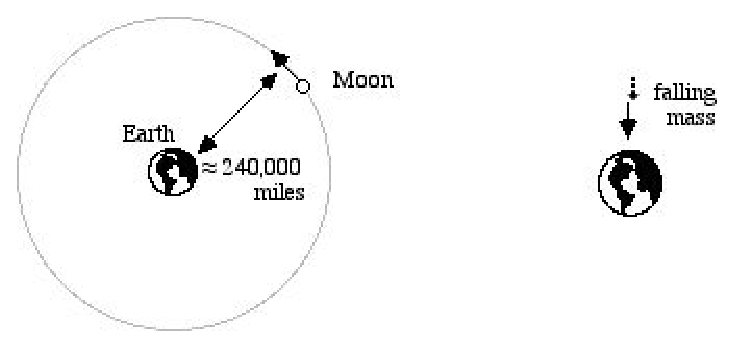
\includegraphics[width=0.9\textwidth]{elec_grav/elec_grav_fig1.eps} 
\end{center}
\answerspace{0.3cm}


\pagebreak[2]
Similarly, the Coulomb force allows us to describe how one charge \char`\"{}falls\char`\"{}
toward another or how an electron orbits a proton in a hydrogen atom. 

\answerspace{0.3cm}
\begin{center}
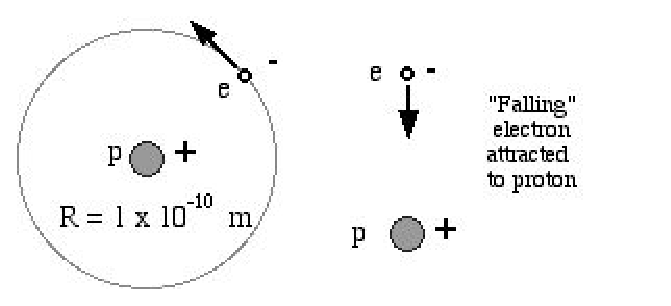
\includegraphics[width=0.9\textwidth]{elec_grav/elec_grav_fig2.eps} 
\end{center}
\answerspace{0.3cm}

The fact that both the Coulomb and the gravitational forces lead to objects
falling and to objects orbiting around each other suggests that these forces
might have the same mathematical form. 

In this unit we will explore the mathematical symmetry between electrical and
gravitational forces for two reasons. First, it is beautiful to behold the unity
that nature offers us as we use the same type of mathematics to predict the
motion of planets and galaxies, the falling of objects, the flow of electrons
in circuits, and the nature of the hydrogen atom and of other chemical elements.
Second, what you have already learned about the influence of the gravitational
force on a mass can be applied to aid your understanding of the forces on charged
particles. 

\textbf{Activity 1: Comparison of Electrical and Gravitational Forces }

Let's start our discussion of this comparison with the familiar expression of
the Coulomb force exerted on charge 1 by charge 2. 

\answerspace{0.3cm}
{\par\centering 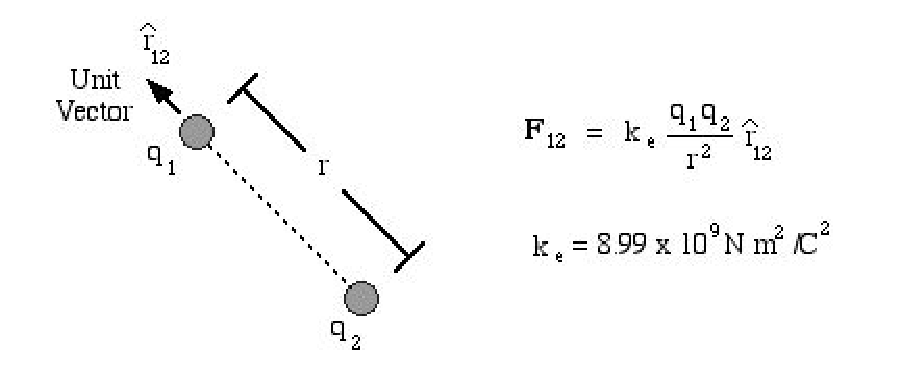
\includegraphics{elec_grav/elec_grav_fig3.eps} \par}
\answerspace{0.3cm}

Charles Coulomb did his experimental investigations of this force in the 18th
century by exploring the forces between two small charged spheres. Much later,
in the 20th century, Coulomb's law enabled scientists to design cyclotrons and
other types of accelerators for moving charged particles in circular orbits
at high speeds. 

Newton's discovery of the universal law of gravitation came the other way around.
He thought about orbits first. This was back in the 17th century, long before
Coulomb began his studies. A statement of Newton's universal law of gravitation
describing the force experienced by mass 1 due to the presence of mass 2 is
shown below in modern mathematical notation: 

\vspace{0.3cm}
{\par\centering 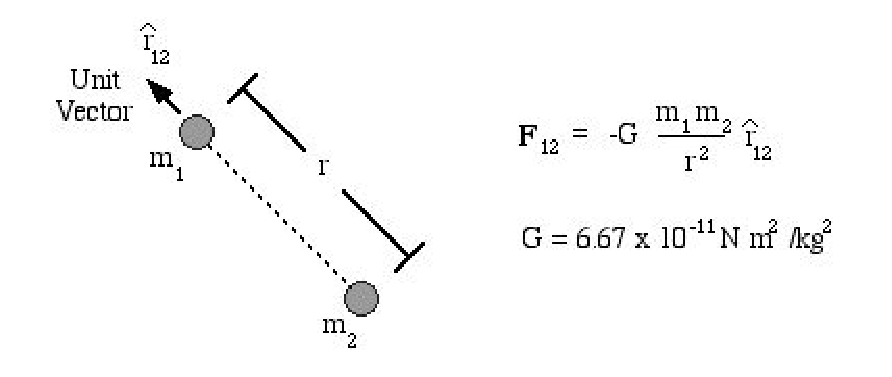
\includegraphics{elec_grav/elec_grav_fig4.eps} \par}
\vspace{0.3cm}

About the time that Coulomb did his experiments with electrical charges in the
18th century, one of his contemporaries, Henry Cavendish, did a direct experiment
to determine the nature of the gravitational force between two spherical masses
in a laboratory. This confirmed Newton's gravitational force law and allowed
him to determine the gravitational constant, G. A fact emerges that is quite
amazing. Both types of forces, electrical and gravitational, are very similar.
Essentially the same mathematics can be used to describe orbital and linear
motions due to either electrical or gravitational interactions of the tiniest
fundamental particles or the largest galaxies. This statement needs to be qualified
a bit when electrons, protons and other fundamental particles are considered.
A new field called quantum mechanics was developed in the early part of this
century to take into account the wave nature of matter, which we don't actually
study in introductory physics. However, even in wave mechanical calculations
electrical forces like those shown above are used. 

\textbf{Activity 2: The Electrical vs. the Gravitational Force} 

Examine the mathematical expression for the two force laws.

(a) What is the same about the two force laws?
\answerspace{20mm}

(b) What is different? For example, is the force between two like masses attractive
or repulsive? How about two like charges? What part of each equation determines
whether the like charges or masses are attractive or repulsive?
\answerspace{20mm}

(c) Do you think negative mass could exist? If there is negative mass, would
two negative masses attract or repel?
\answerspace{20mm}

\textbf{Which Force is Stronger-- Electrical or Gravitational?} 

Gravitational forces hold the planets in our solar system in orbit and account
for the motions of matter in galaxies. Electrical forces serve to hold atoms
and molecules together. If we consider two of the most common fundamental particles,
the electron and the proton, how do their electrical and gravitational forces
compare with each other?

Let's peek into the hydrogen atom and compare the gravitational force on the
electron due to interaction of its mass with that of the proton to the electrical
force between the two particles as a result of their charge. In order to do
the calculation you'll need to use some well known constants.

Electron: m\( _{e} \) = 9.1 x 10\( ^{-31} \) kg, q\( _{e} \) = - 1.6 x 10\( ^{-19} \)
C 

Proton: m\( _{p} \) = 1.7 x 10\( ^{-27} \) kg, q\( _{p} \) = +1.6 x 10\( ^{-19} \)
C 

Distance between the electron and proton: r = 0.53 x 10\( ^{-10} \) m

\textbf{Activity 3: The Electrical vs. the Gravitational Force in the Hydrogen
Atom}

(a) Calculate the magnitude of the electrical force on the electron. Is it attractive
or repulsive?
\answerspace{20mm}

(b) Calculate the magnitude of the gravitational force on the electron. Is it
attractive or repulsive?
\answerspace{20mm}

(c) Which is larger? By what factor (i.e. what is the ratio)?
\answerspace{20mm}

(d) Which force are you more aware of on a daily basis? If your answer does
not agree with the result of part (c), explain why, i.e. why do we usually not 
experience electrical forces in our everyday lives?
\answerspace{20mm}

\textbf{Activity 4: The Gravitational Force of the Earth}

(a) Use Newton's law to show that the magnitude of the acceleration due to gravity
on an object of mass m at a height h above the surface of the earth is given by
the following expression:
\[
\frac{GM_{e}}{\left( R_{e}+h\right) ^{2}}\]

Hint: Because of the spherical symmetry of the Earth you can treat the mass
of the Earth as if it were all concentrated at a point at the Earth's center.
\answerspace{20mm}
\pagebreak

(b) Calculate the acceleration due to gravity of a mass m at the surface of
the earth (h=0). The radius of the earth is R\( _{e} \) \( \approx  \) 6.38
x 10\( ^{3} \) km and its mass M\( _{e} \) \( \approx  \) 5.98 x 10\( ^{24} \)
kg. Does the result look familiar? How is this acceleration related to the gravitational
acceleration g?
\vspace{40mm}

(c) Use the equation you derived in part (a) to calculate the acceleration due
to gravity at the ceiling of the room you are now in. How does it differ from
the value at the floor? Can you measure the difference in the lab using the
devices available?
\vspace{30mm}

(d) Suppose you travel halfway to the moon. What is the new value of the acceleration due to gravity (neglecting the effect of the moon's pull)? (Recall that the earth-moon distance is about 384,000 km.)
\vspace{30mm}

(e) Is the gravitational acceleration \char`\"{}constant\char`\"{}, g, really
a constant? Explain.
\vspace{30mm}

(f) In part (d) you showed that there is a significant gravitational attraction
halfway between the earth and the moon. Why, then, do astronauts experience
``weightlessness'' when they are orbiting a mere 120 km above the earth?



\section{The Electric Field Near a Charged Rod}

\instructornote{%
By Matt, added to manual Fall 2015.  Time: $\sim$45 minutes
}

\makelabheader %(Space for student name, etc., defined in master.tex)

\begin{wrapfigure}[10]{r}{0.385\textwidth}
\vspace{-.25in}
\hspace{0.13in}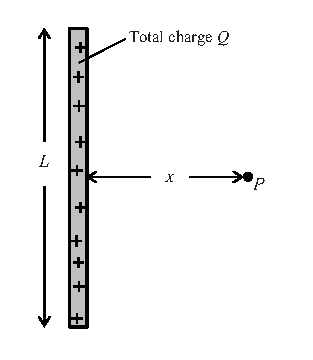
\includegraphics{electric_field_near_a_charged_rod/fig1.eps}
\end{wrapfigure}

\vspace{1cm}

\textbf{Objective and statement of the problem:}

Calculate the electric field $\vec{E}$ at a point $P$ a distance $x$ away from the midpoint of a thin rod
of length $L$ and total charge $Q$.

\vspace{1cm}

\textbf{Introduction and outline of solution:}

Think of the rod as a bunch of teeny-tiny little point charges $dQ$ arranged in a column. You will solve this problem by calculating the sum (actually an integral) of the electric fields due to each point charge.  In the second figure, below, we have added a set of coordinate axes, and defined a tiny bit of charge $dQ$ that is on a tiny bit of length $dy$.  
\par

\begin{wrapfigure}[6]{r}{0.4\textwidth}
\vspace{-.55in}
   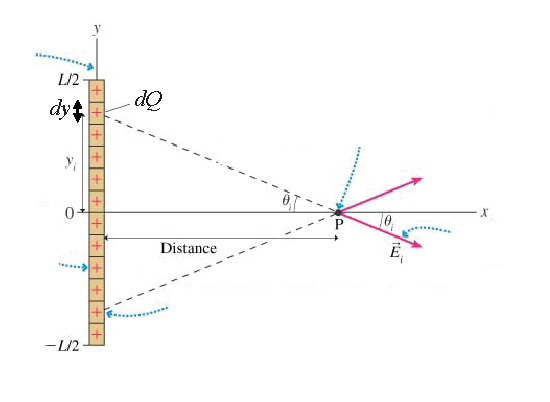
\includegraphics{electric_field_near_a_charged_rod/fig2.eps}
\end{wrapfigure}

%\vspace{0.1cm}
%{\centering \resizebox*{0.5\textwidth}{!}{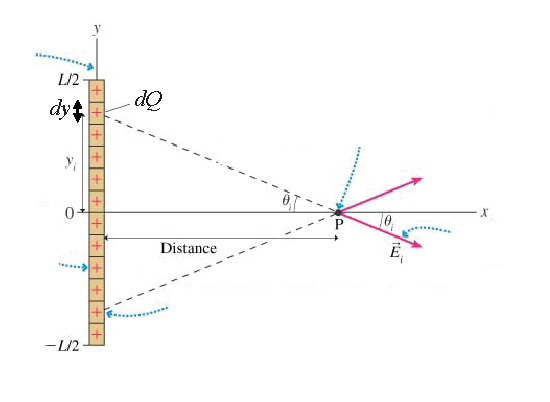
\includegraphics{electric_field_near_a_charged_rod/fig2.eps}} \par}

\par
\vspace{0.5cm}
\par
\textbf{Step 1:} \newline
In words, what is the approximate direction of the electric field at point $P$ due to just the one little bit of charge $dQ$ shown?

\vspace{.6in}

What is the direction of the electric field at point $P$ due to the whole rod?  How do you know?

\vspace{.6in}

\textbf{Step 2:} \newline
What is the magnitude of the electric field $|d\vec{E}|$  due to just the bit of charge $dQ$?  (Write the relevant distance in terms of $x$ and $y$, not $\theta$.)
\[
|d\vec{E}|=\hspace{0.7in}
\]
\vspace{.3in}

\textbf{Step 3:} \newline
What is the magnitude of the $x$-component of   $d\vec{E}$?  (It's similar to your answer above but with an extra $\sin \theta$ or $\cos \theta$.) 
\[
d{E}_x=\hspace{1in}
\]
\vspace{.3in}

\pagebreak
\textbf{Step 4:} \newline
Rewrite the last step, giving  $\sin \theta$ or $\cos \theta$ in terms of a ratio involving $x$, $y$, and/or $\sqrt{x^2 + y^2}$.
\[
d{E}_x=\hspace{1in}
\]
\vspace{.3in}

\textbf{Step 5:} \newline
The linear charge density $\lambda$ of the rod is given by $\lambda = Q/L$.  Write $dQ$ in terms of $\lambda$  and $dy$, then in terms of $Q$, $L$ and $dy$.
\[
dQ=\hspace{0.7in}=\hspace{0.7in}
\]
\vspace{.3in}

\textbf{Step 6:} \newline
Combine your answers to steps 4 and 5 to write $\vec{E}$ as a single integral over $dy$ which you can solve.  What are the limits of the integral?
\[
\vec{E}=\int d\vec{E}_x=\hspace{1.5in}
\]
\vspace{.3in}

\textbf{Step 7:} \newline
Evaluate the integral.  
\[
\vec{E}=\hspace{2in}
\]

 \vspace{3in}

\textit{Note: one of the following might be helpful:}
\begin{flalign*}
& \int \! \frac{1}{\left (u^2 + a^2 \right )^\frac{3}{2}} \, du=\frac{u}{a^2 \sqrt{u^2 + a^2}} &\\
& \int \! \frac{u}{\left (u^2 + a^2 \right )^\frac{3}{2}} \, du=\frac{-1}{\sqrt{u^2 + a^2}} \\
& \int \! \frac{1}{u^2 + a^2} \, du=\frac{1}{a} \tan^{-1} \frac{u}{a}
\end{flalign*}
%\]




\section{The Electric Potential\footnote{%
1990-93 Dept. of Physics and Astronomy, Dickinson College. Supported
by FIPSE (U.S. Dept. of Ed.) and NSF. Portions of this material may
have been modified locally and may not have been classroom tested
at Dickinson College.
}}

\makelabheader %(Space for student name, etc., defined in master.tex)

\bigskip
\textbf{Overview}

It takes work to lift an object in the earth's gravitational field.
Lowering the object releases the energy that was stored as potential
energy when it was lifted. Last semester, we applied the term \emph{conservative}
to the gravitational force because it {}``releases'' \underbar{all}
of the stored energy. We found experimentally that the work required
to move a mass in the gravitational field was path independent. This
is an important property of any conservative force. Given the mathematical
similarity between the Coulomb force and the gravitational force,
it should come as no surprise that experiments confirm that an electric
field is also conservative. This means that the work needed to move
a charge from point A to point B is independent of the path taken
between points. A charge could be moved directly between the two points
or looped around and the work expended to take either path would be
the same. Work done by an electric field on a test charge q traveling
between points A and B is given by

{\centering \( W=\int ^{B}_{A} \)\( \overrightarrow{F}\cdot d\overrightarrow{s}=\int ^{B}_{A}q\overrightarrow{E}\cdot d\overrightarrow{s} \)\par}

\bigskip
\textbf{Activity 1: Work Done on a Charge Traveling in a Uniform Electric
Field}

(a) A charge q travels a distance d from point A to point B; the path
is parallel to a uniform electric field of magnitude E. What is the
work done by the field on the charge? How does the form of this equation
compare to the work done on a mass m traveling a distance d in the
almost uniform gravitational field near the surface of the earth?

\vspace{0.3cm}
{\centering \resizebox*{0.2\textwidth}{!}{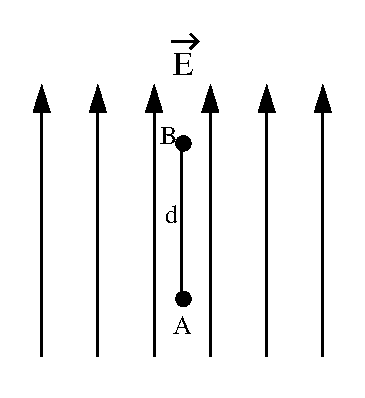
\includegraphics{electric_potential/electric_potential_fig_1.eps}} \par}
\answerspace{0.3cm}

(b) The charge $q$ travels a distance $d$ from point $A$ to point $B$ in a
uniform electric field of magnitude $E$, but this time the path is perpendicular
to the field lines. What is the work done by the field on the charge?

\vspace{0.3cm}
{\centering \resizebox*{0.2\textwidth}{!}{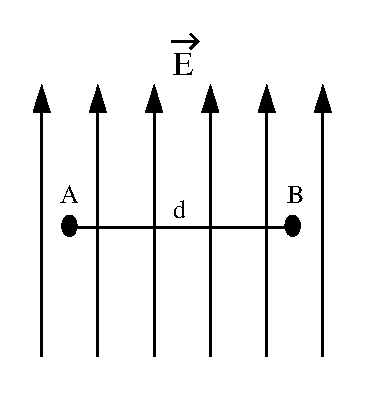
\includegraphics{electric_potential/electric_potential_fig_2.eps}} \par}
\answerspace{0.3cm}

\pagebreak[2]
(c) The charge $q$ travels a distance $d$ from point $A$ to point $B$ in a
uniform electric field of magnitude $E$. The path lies at a 45\( ^{\circ } \)
angle to the field lines. What is the work done by the field on the
charge?

\vspace{0.3cm}
{\centering \resizebox*{0.2\textwidth}{!}{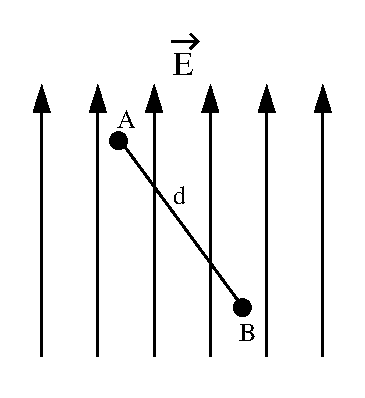
\includegraphics{electric_potential/electric_potential_fig_3.eps}} \par}
\answerspace{0.5cm}

\textbf{Potential Energy and Potential Difference}

Recall that by definition the work done by a conservative force equals
the negative of the change in potential energy, so that the change
in potential energy of a charge moving from point $A$ to point $B$ under
the influence of an electrical force is given by:

{\centering \( \Delta U=U_{B}-U_{A}=-\int ^{B}_{A}q\overrightarrow{E}\cdot d\overrightarrow{s} \)\par}

By analogy to the definition of the electric field, we are interested
in defining the \emph{electric potential difference} \( \Delta V=V_{B}-V_{A} \)
as the change in electric potential energy \( \Delta U \) per
unit charge. Formally, \emph{the potential difference is defined as
the work per unit charge that an external agent must perform to move
a test charge from A to B without changing its kinetic energy}. The
potential difference has units of joules per coulomb. Since 1 J/C
is defined as one \emph{volt}, the potential difference is often referred
to as \emph{voltage}.

\textbf{Activity 2: The Equation for Potential Difference}

Write the equation for potential difference as a function of \( \overrightarrow{E} \),
\( d\overrightarrow{s} \), $A$, and $B$.
\answerspace{15mm}

\textbf{The Potential Difference for a Point Charge}

The simplest charge configuration that can be used to consider how
voltage changes between two points in space is a single point charge.
We will start by considering a single point charge and then move on
to more complicated configurations of charge.

A point charge $q$ produces an electric field that points radially outward
in all directions for a positive charge, radially inward for a negative charge. The line integral equation for the potential difference
can be evaluated to find the potential difference between any two
points in space $A$ and $B$ (a line integral is one that follows a path
through space).

It is common to choose the reference point for the determination of
voltage to be set at infinity so that we are determining the work
per unit charge that is required to bring a test charge from infinity
to a certain point in space. Let's choose a coordinate system so that
the point charge is conveniently located at the origin. In this case
we will be interested in the potential difference between infinity
and some point which is a distance r from the point charge. Thus,
we can write the equation for the potential difference, or voltage,
as

{\centering \( \Delta V=V_{B}-V_{A}=V_{r}-V_{\infty }=-\int ^{r}_{\infty }\overrightarrow{E}\cdot d\overrightarrow{s} \)\par}

Often, when the reference point for the potential difference is at
infinity, this difference is simply referred to as {}``the potential'',
and the symbol \( \Delta V \) is just replaced with the symbol $V$.

\pagebreak[2]
\textbf{Activity 3: Potential at a Distance r from a Charge}

Starting from the expression for the electric field of a point charge,
show that, if $A$ is at infinity and $B$ is a distance $r$ from a point
charge $q$, then the potential $V$ is given by the expression

{\centering \( V=\frac{kq}{r} \)\par}

where \( k=\frac{1}{4\pi \varepsilon _{\circ }} \)= 8.99 x 10\( ^{9} \)
Nm\( ^{2} \)/ C\( ^{2} \).
\textbf{Hint:} What is the mathematical expression for an $E$-field
from a point charge?

%\vspace{0.3cm}
%{\centering \resizebox*{0.4\textwidth}{!}{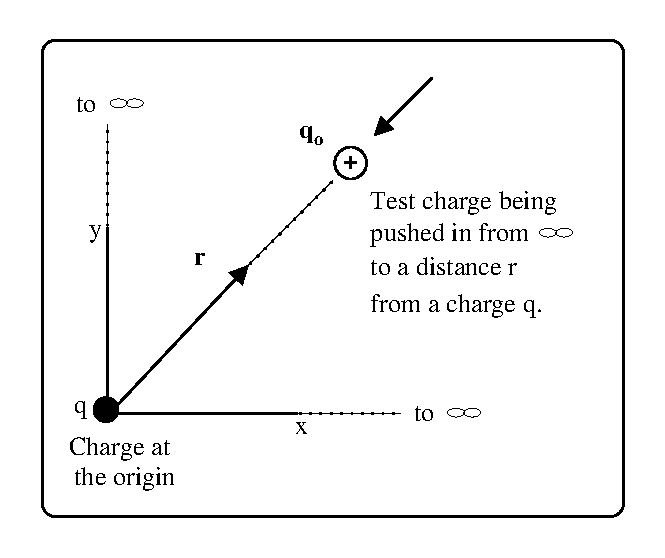
\includegraphics{electric_potential/electric_potential_fig_4.eps}} \par}
{\resizebox*{0.4\textwidth}{!}{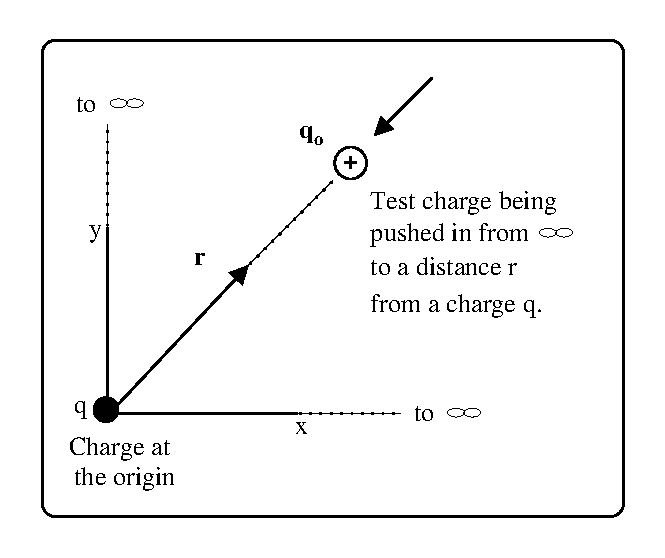
\includegraphics{electric_potential/electric_potential_fig_4.eps}} \par}
%\vspace{0.3cm}

\answerspace{15mm}

\textbf{Activities 4 and 5: Potential Due to Continuous Charge Distributions}

The potential from a continuous charge distribution can be calculated
several ways. Each method should yield approximately the same result.
First, we can use an integral method in which the potential $dV$ from
each element of charge $dq$ is integrated mathematically to give a total
potential at the location of interest. Second, we can approximate
the value of the potential $V$ by summing up several finite elements
of charge \( \Delta q \) by using a computer spreadsheet or hand
calculations.

Again, let's consider a relatively simple charge distribution. In
this case we will look at a ring with charge uniformly distributed
on it. We will calculate the potential on the axis passing through
the center of the ring as shown in the diagram below. (Later on you
could find the potential difference from a disk or a sheet of charge
by considering a collection of nested rings).

\vspace{0.3cm}
{\centering 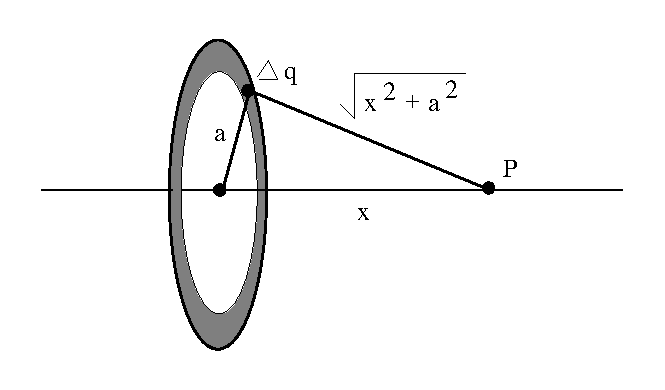
\includegraphics[scale=0.8]{electric_potential/electric_potential_fig_5.eps} \par}
\vspace{0.3cm}

\vspace{2in}
A ring of charge has a total charge of $Q = 20$\( \mu  \)C (i.e. 20
x 10\( ^{-6} \) C). The radius of the ring, $a$, is 30 cm. We want
to find the electric field and the electric potential at a distance $x$ from the ring along an axis that is perpendicular to the ring
and passes through its center. Let's begin by calculating the potential
in the next activity.

\textbf{Hints:} Since the potential is a scalar and not a vector we
can calculate the potential at point $P$ (relative to \( \infty  \))
for each of the charge elements \( \Delta q \) and add them to each
other. This looks like a big deal but it is actually a trivial problem
because all the charge elements are the same distance from point $P$.

\textbf{Activity 4: Numerical Estimate of the Potential due to a Charged
Ring}

(a) Divide the ring into 20 elements, each of charge \( \Delta q \) = 1.0 x 10\( ^{-6} \) C and
calculate the total $V$ at a distance of $x$ = 20 cm from the center of
the ring using a spreadsheet program or by hand calculation. Summarize
the result below. Be sure to attach a printout of your spreadsheet
results.
\answerspace{1.25in}

\textbf{Activity 5: Calculation of the Potential due to a Charged Ring}

By following the steps below, you can use an integral to find a more
exact value of the potential.

(a) Show that

{\centering \( V=k\int \frac{dq}{r}=k\int \frac{dq}{\sqrt{x^{2}+a^{2}}} \)\par}
\answerspace{20mm}

(b) Explain why

{\centering \( k\int \frac{dq}{\sqrt{x^{2}+a^{2}}}=\frac{k}{\sqrt{x^{2}+a^{2}}}\int dq \)\par}

(i.e. explain why \( \sqrt{x^{2}+a^{2}} \) can be pulled out of the integral).
\answerspace{20mm}

(c) Perform the integration in part (b) above. Then substitute values
for $a$, $x$, and $Q$ into the resulting expression in order to obtain a
more {}``exact'' value for the potential.
\answerspace{25mm}

(d) How does the {}``numerical'' value that you obtained in Activity
4 compare with the {}``exact'' value you obtained in (c)?
\answerspace{10mm}

\pagebreak[2]
Now let's take a completely different approach to the same problem.
If we can find the vector equation for the electric field at point
P due to the ring of charge, then we can use the expression

{\centering \( \Delta V=V_{r}-V_{\infty }=-\int ^{r}_{\infty }\overrightarrow{E}\cdot d\overrightarrow{s} \)\par}

as an alternative way to find a general equation for the potential
at point $P$.

\answerspace{0.3cm}
{\centering 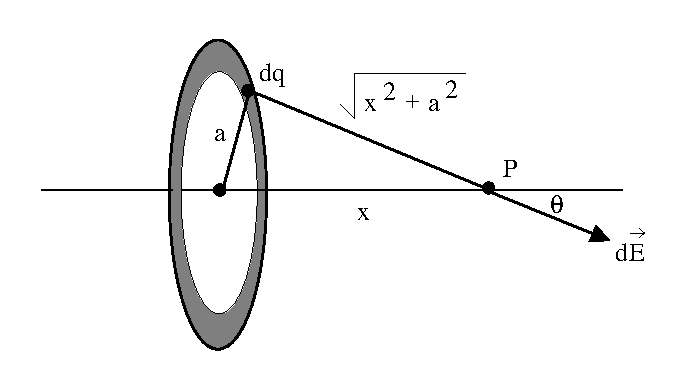
\includegraphics[scale=0.8]{electric_potential/electric_potential_fig_6.eps} \par}
\answerspace{0.3cm}

\textbf{Activity 6: \( \Delta  \)V from a Ring Using the E-field
Method}

(a) Starting from the electric field of a point charge, show that
the electric field at point P from the charged ring is given by

{\centering \( \overrightarrow{E}=\frac{kqx}{(x^{2}+a^{2})^{3/2}}\hat{x} \)\par}

\textbf{Hints:} (1) Why is there no y component of the E-field? (2)
\( \cos \theta =\frac{x}{\sqrt{x^{2}+a^{2}}} \)
\answerspace{30mm}

(b) To find \( \Delta  \)V use the following equation.

{\centering \( \Delta V=V_{r}-V_{\infty }=-\int ^{r}_{\infty }\overrightarrow{E}\cdot d\overrightarrow{s} \)\par}
\textbf{Hint:} You will probably need to consult the integral tables in the appendix of your text.
\textbf{Note:} The above expression for $\overrightarrow{E}$ is only valid along the $x$-axis.
\answerspace{30mm}

(c) How does the result compare to that obtained in Activity 5 (c)?
\answerspace{10mm}

\pagebreak[2]
\textbf{Equipotential Surfaces}

Sometimes it is possible to move along a surface without doing any
work. Thus, it is possible to remain at the same potential energy
anywhere along such a surface. If an electric charge can travel along
a surface without doing any work, the surface is called an \emph{equipotential
surface}.
Consider the three different charge configurations shown below. Where
are the equipotential surfaces? What shapes do they have?

\textbf{Hint:} If you have any computer simulations available to you
for drawing equipotential lines associated with electrical charges,
you may want to check your guesses against the patterns drawn in one
or more of the simulations.

\textbf{Activity 7: Sketches of Electric Field Lines and Equipotentials}

(a) Suppose that you are a test charge and you start moving at some
distance from the charge below (such as 4 cm). What path could you
move along without doing any work, i.e. \( \overrightarrow{E}\cdot d\overrightarrow{s} \)
is always zero? What is the shape of the equipotential surface? Remember
that in general you can move in \emph{three} dimensions.

%\vspace{0.3cm}
{\centering \resizebox*{0.27\columnwidth}{!}{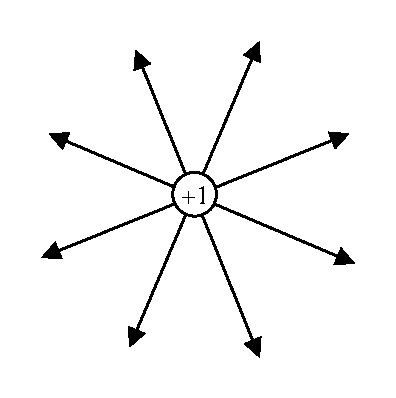
\includegraphics{electric_potential/electric_potential_fig_7.eps}} \par}
%\vspace{0.3cm}

(b) Find some equipotential surfaces for the charge configuration
shown below, which consists of two charged metal plates placed parallel
to each other. What is the shape of the equipotential surfaces?

%\vspace{0.3cm}
{\centering \resizebox*{0.26\textwidth}{!}{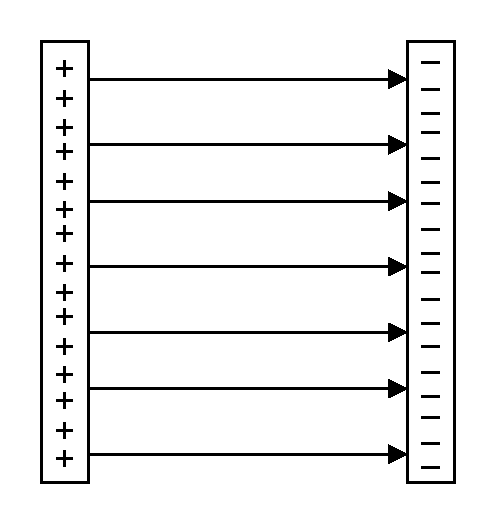
\includegraphics{electric_potential/electric_potential_fig_8.eps}} \par}
%\vspace{0.3cm}

(c) Find some equipotential surfaces for the electric dipole charge
configuration shown below.

\vspace{0.3cm}
{\centering \resizebox*{0.24\textwidth}{!}{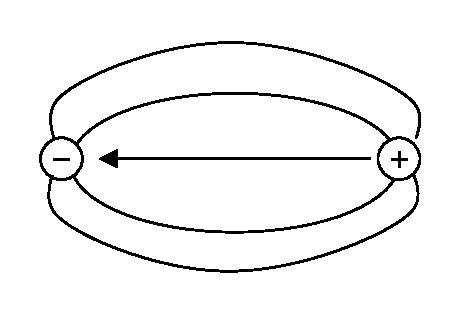
\includegraphics{electric_potential/electric_potential_fig_9.eps}} \par}
\vspace{0.3cm}

(d) In general, what is the relationship between the direction of
the equipotential lines you have drawn (representing that part of
the equipotential surface that lies in the plane of the paper) and
the direction of the electric field lines?
\answerspace{10mm}



\section{Measuring Equipotential Lines and Electric Fields}

\makelabheader %(Space for student name, etc., defined in master.tex)

%\textbf{Objective}
%\begin{itemize}
%\item To learn the shape of electric fields.
%\end{itemize}

\bigskip
\textbf{Apparatus}
%\vspace{-\parskip}
\begin{itemize}[nosep]
\item Power supply
\item Voltmeter
\item Conducting sheets
\item Carbon and white paper
\item Cork board and pins
\end{itemize}

\medskip

\textbf{Introduction}

Charged objects exert an electrical force on other charged objects
in proportion to the amount of charge each has, just as massive objects
exert a gravitational force on one another in proportion to their
masses. The magnitudes of both forces depend, too, on the distance
between objects. However, whereas the gravitational force is always
attractive, electrical forces may be either attractive or repulsive
depending on the sign of the charges. It is convenient in understanding
the nature of electrical forces to draw pictures of them. We represent
the fields, which provide the magnitude and direction of the forces,
as lines. We agree on a convention: the direction of the field is
that of the force on an infinitesimal positive test charge. Thus,
the lines of force originate on and come out of positive charges and
are directed toward and terminate on negative charges (see figure
below). The magnitude of the field, and therefore the force, is proportional
to the density of the field lines.

{\centering 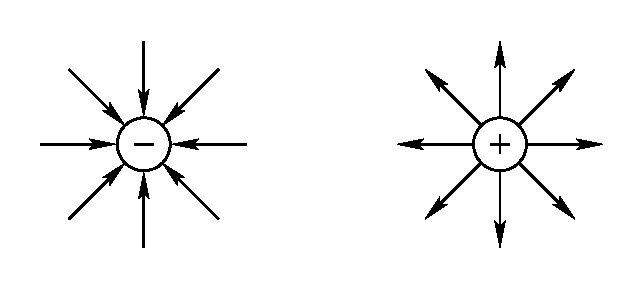
\includegraphics[height=1.6in]{electric_fields_and_equipotential_lines/ef_equipot_lines_fig_1.eps} \par}

Please note that when the situation is electrostatic, 1) the electric
field within a metal is zero, and 2) the electric field just outside
the surface of a metal is perpendicular to the surface. If either
of these conditions were altered, then there would be an electric
current in the metal, which is not an electrostatic situation. Because
an electric field exerts a force on a charge, work must be done to move a
charged object along any of the field lines. On the other hand, movement
perpendicular to the field lines requires no work. Such movement is
said to be along an equipotential line.

{\centering 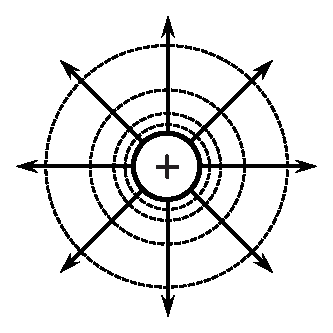
\includegraphics[height=1.6in]{electric_fields_and_equipotential_lines/new_ef_fig_2.eps} \par}

In the figure above, the electric field for a positive point charge
is shown as lines with arrows. The regions of equipotential (equipotential
lines) are shown with circles. Notice that the equipotential lines
are perpendicular to the electric field lines and that the density
of equipotential lines is proportional to the electric field strength.

\pagebreak[2]

Electric field lines are difficult to measure directly, but potentials
can be measured with a voltmeter. An electric field will arise in
the space surrounding two separated charged conductors. With one lead
of a voltmeter connected to one of the conductors and the other used
as a probe, the potentials can be determined (see figure below).

\vspace{0.3cm}
{\centering \resizebox*{0.9\textwidth}{!}{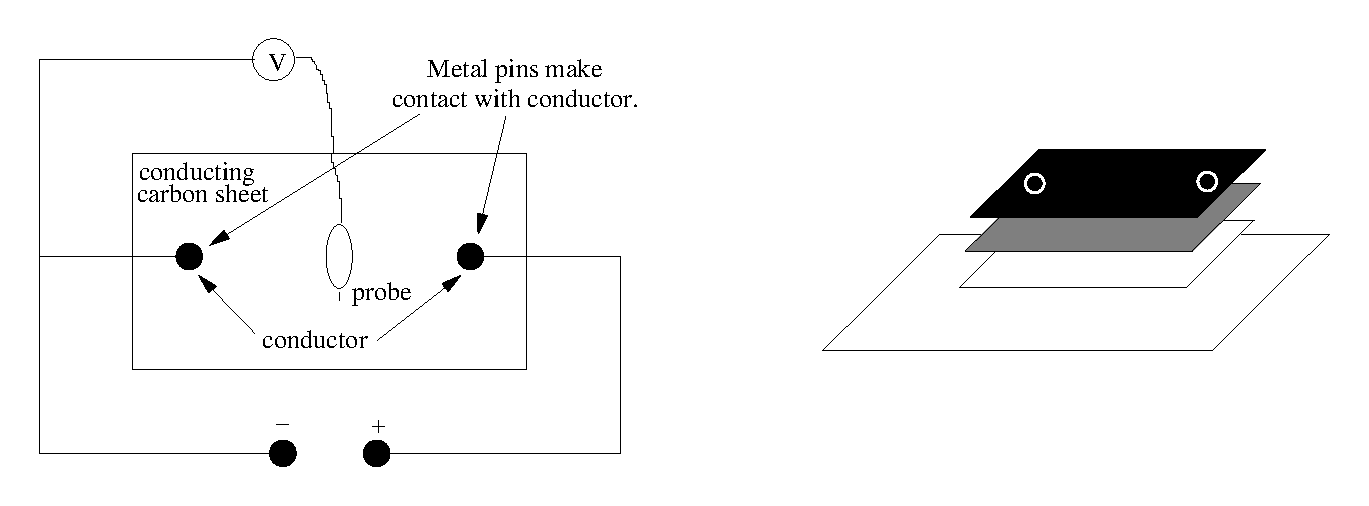
\includegraphics{electric_fields_and_equipotential_lines/ef_equipot_lines_fig_3.eps}} \par}
\vspace{0.3cm}

\textbf{Activity 1: Field Lines for Two Point Charges}

\begin{enumerate}[labparts]
\item\textbf{Prediction:} Using the rules given in the introduction and
given in the first set of figures, draw the electric field lines for two
oppositely charged point objects. Sketch the equipotential lines.
\answerspace{1in}

\item Find the conducting paper with the two silver circles on the front
and lay it over a copy carbon and a sheet of paper on top of the cork
board.
\item Connect the positive output of the power supply to one of the circles
and the negative to the other. NOTE: Push pins must be pushed down HARD on the 
conducting ink of the circles.
\item Connect the negative lead of the voltmeter to the negative conductor
and use the positive lead as the probe. 
\item With the power supply voltage turned on and set to 20 volts, probe
lightly with the voltmeter to find a number of points on the carbon
paper registering 16 volts. Hold the probe at an angle so that more area of the 
point will be in contact with the conducting paper. This will minimize 
uncertainty in the reading. Push down each time you find a point so
that marks will be made on the bottom paper.
\item Repeat for 12 volts, 8 volts, and 4 volts.
\item You should end up with a series of dots on your sheet of paper. Connect
those associated with the same potential with smooth lines. Label each line 
with its associated voltage.
\item Recalling the relationship between electric field lines and equipotential
lines, sketch in the electric field lines. (\emph{Other group members
can sketch copies of the same results.})
\item Does your experimental result agree with your prediction? Explain.
\answerspace{15mm}

\end{enumerate}

\pagebreak[2]
\textbf{Activity 2: Field Lines for Two Parallel Plates}

\begin{enumerate}[labparts]
\item Draw what you \textit{predict} the field lines and equipotential
lines between parallel plates will look like.
\answerspace{1.2in}

\item Carry out the instructions from Activity 1 to check your prediction.  Draw a sketch of your results below.
\answerspace{1.2in}

\item Does your result agree with your prediction? Explain.
\answerspace{.5in}

\end{enumerate}
\textbf{Activity 3: Field Lines Between a Point Charge and a Plate}

\begin{enumerate}[labparts]

\item Draw what you \textit{predict} the field lines and equipotential
lines between a point charge and a parallel plate will look like.
\answerspace{1.2in}

\item Map the field lines as before, andraw a sketch of your results below.
\answerspace{1.2in}

\item Does your result agree with your prediction? Explain.
\answerspace{.5in}

\item If the potential is zero, must the electric field be zero as well?
\answerspace{.3in}
%\item What can you say about the electric field along an equipotential line?\vspace{15mm}

\end{enumerate}
%\textbf{Activity 4: Field Lines for a Plate and a Charged Circle}

%\textbf{Prediction:} Sketch what you think the field and potential
%lines between a charged circle and a plate look like.
%\vspace{1in}

%\begin{enumerate}
%\item Determine the field lines.
%\item What is the field strength within a charged, continuous surface?\vspace{15mm}
%\end{enumerate}




\section{The Electric Field and the Electric Potential I}

\makelabheader %(Space for student name, etc., defined in master.tex)

\textbf{Objective}

\begin{itemize}
\item To investigate the electric field and potential of a point charge.
\end{itemize}

\textbf{Apparatus}

\begin{itemize}
\item Electric field and potential simulation entitled {\it EMField}.
\end{itemize}

\textbf{Introduction}

The direction of an electric field is the direction of the force on
a tiny positive test charge placed in the region of space where the
field is to be measured. If the magnitude of this test charge is infinitesimally
small, so small that it will not displace or disturb the charges that
are the source of the field, we can use the test charge to determine
quantitatively the strength of the electric field. The strength of
the electric field is taken to be the electric force, $F$, on the test
charge divided by the magnitude of the test charge, \( q_{t} \):
\( E=\frac{F}{q_{t}} \). The force (Coulomb's Law) between two charges,
\( q_{1} \) and \( q_{2} \), is \( F=k\frac{q_{1}q_{2}}{r^{2}} \),
where \( k \)= 9 x 10\( ^{9} \) Nm\( ^{2} \)/C\( ^{2} \). The units
of \( E \) are newtons per coulomb, so another way of describing the field
strength is to say it is the force experienced by a unit positive
test charge.

Recall from a previous laboratory exercise that the potential difference
between two points A and B, V\( _{B} \) - V\( _{A} \), is the work
done carrying a unit positive charge from point A to point B. Also,
the lines of force (the electric field lines) are always perpendicular
to the equipotential lines, lines on which all points are at the same
potential. In a static electric field, the electric potential difference
between two points is a constant and does not depend on the path used
for its computation. The absolute potential, as opposed to the potential
difference, is the amount of work done in carrying a unit charge from
infinity to point B. The magnitude of the absolute potential, then,
is computed as the integral from infinity to the point B of the electric
field.

\textbf{Investigation 1: A Single Charge}

\textbf{Activity 1: The Electric Field}

(a) (Note: you will need to run the program \filename{EMField} on a ``virtual machine''; see Appendix \ref{virtual_machine}.)  Go to \filename{Start $\rightarrow$ Programs $\rightarrow$ Physics Applications} and open the program \filename{EMField}. 
Click on the screen and you will see a screen with a set of
instructions.
Go to the \textbf{Sources} menu and select \textbf{3D Point Charges}.
A blank `table top' with a set of menu 
buttons at the top and bottom will appear. See Figure 1 below.

\begin{figure}[hbt]
\begin{center}
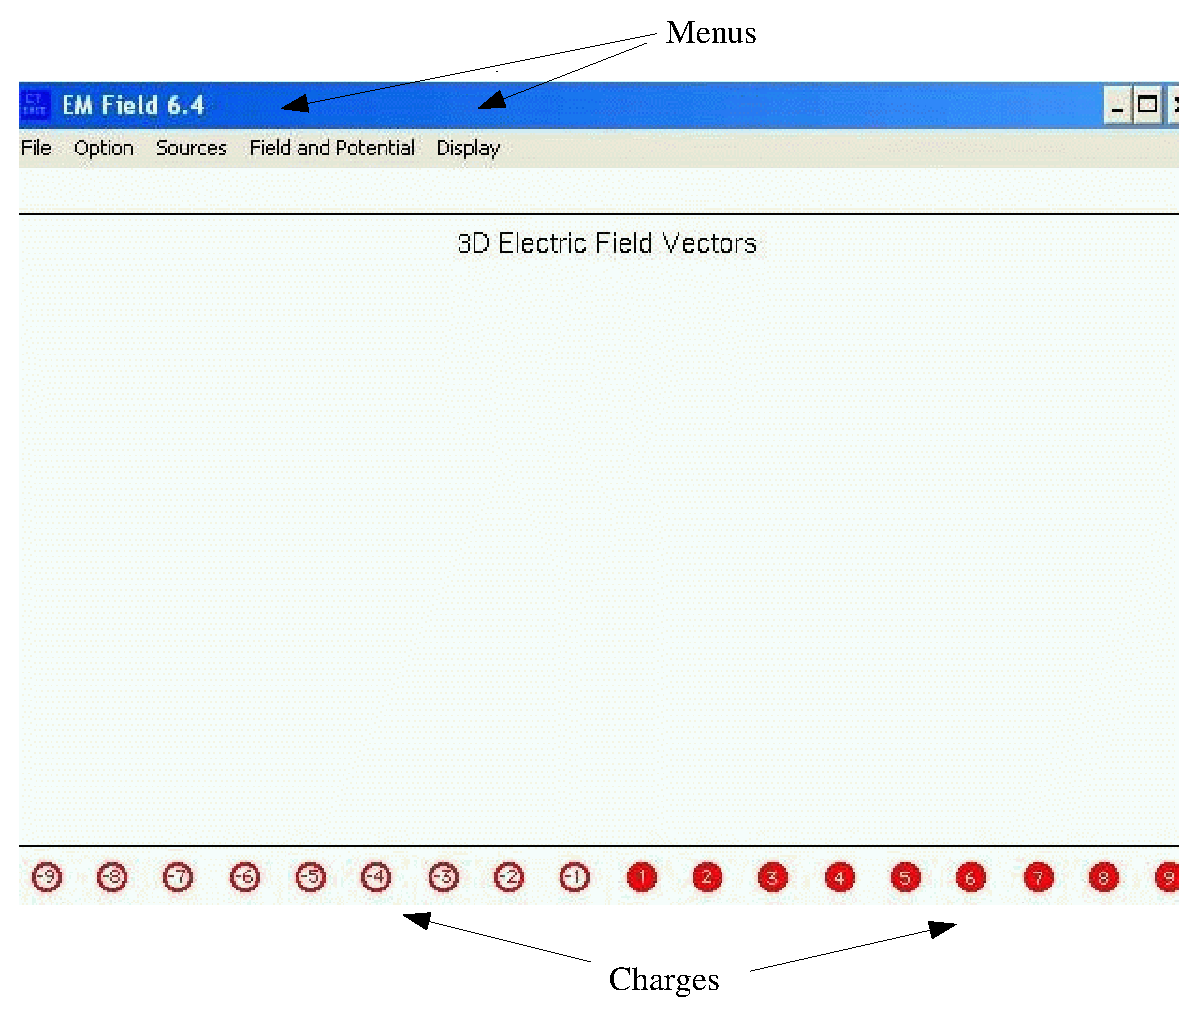
\includegraphics[height=4.0in]{electric_field_and_electric_potential/emfield1c.eps}
\caption{Table top for {\it EMField.}}
\index{color page}
\end{center}
\end{figure}

(b) Go to the {\bf Display} menu and set {\it EMField} to
{\bf Show Grid} and {\bf Constrain to Grid}.
These choices will make the following investigation a bit easier to perform.

(c) Select
the charge labeled {}``+4'' from the available set by clicking
on it and dragging it to the center of the table top. 

(d) \textbf{Prediction}: You will take measurements of the field at different
distances from the charge. You know the relative size of the
charge (+4), but you don't know the size of the charge in coulombs.
Generate an expression for the magnitude of the field from an unknown charge
with appropriate numerical constants and units.
The only unknown in your result should be the charge in coulombs.
How does the electric field depend on $r$, the distance from the point charge?
%\vspace{15mm}
\newpage

(e) Click anywhere in the table top and you will see an arrow drawn.
The size and direction of the arrow represent the magnitude and direction of
the electric field at that point due to the `+4' charge.
In what direction does the arrow point?
Click on the opposite side of the table top.
In what direction does this arrow point? How is it related to the first arrow?
\vspace{15mm}

(f) Click on many points so that you get a wide range of magnitudes from large
(barely fits on the table top) to small (barely bigger than a dot).

(g) Print the table top and use a ruler to measure the distance of each field 
point from the charge and the lengths of each of the arrows on your plot. 
Enter these data in the table below. Use the scale at the bottom of the table 
top to convert the length of each arrow into an electric field magnitude.
The units of the scale electric field vector are $1.0 ~ N/C$.

\vspace{0.3cm}
{\centering \begin{tabular}{|c|c|c|c|}
\hline 
~~~Distance from Charge (cm)~~~&
~~~Arrow Length (cm)~~~&
~~~Measured E (N/C)~~~\\
\hline
\hline 
&
&
\\
\hline 
&
&
\\
\hline 
&
&
\\
\hline 
&
&
\\
\hline 
&
&
\\
\hline 
&
&
\\
\hline 
&
&
\\
\hline 
&
&
\\
\hline 
&
&
\\
\hline
\end{tabular}\par}
\vspace{0.3cm}

%(h) Use the results in column 3 of your table to determine the unknown charge for each electric field measurement and enter the results in the table. NOTE: 
%For this calculation, assume the Coulomb's Law constant $k = 1.00 Nm^{2}/C^{2}$.
%This makes the charge a factor of about $10^{10}$ bigger than it is supposed to 
%be, but we are focussing here on how the electric field varies with distance 
%from the charge. Calculate the average and standard deviation of the values 
%of the charge. Are your results consistent? Explain.
%\vspace{30mm}

(h) \textbf{Prediction}: From Coulomb's Law, we expect the spatial variation
of the field strength to obey a power law: \( \left| E\right| =Ar^{n} \),
where \( A \) and \( n \) are constants. What do you predict the value of 
\( n \) to be?\vspace{15mm}

(i) Graph field strength as a function of $r$. Using the power fitting
function, determine the power of the function, $n$, and record it here.
Attach the plot to this unit.
\vspace{15mm}

(j) Does your result agree with your prediction? Explain any discrepancy.
\vspace{15mm}

\vspace{0.5in}
\textbf{Activity 2: The Electric Potential}

(a) Under the {\bf Display} menu click on {\bf Clean up Screen} to erase the
electric field vectors.

(b) \textbf{Prediction}: You will now take measurements of the potential.
How do you expect the electric potential to change with distance from the point
charge?
\vspace{15mm}
 
(c) Click on the \textbf{Potential} option under the \textbf{Field and Potential} menu. Click on the table top and a marker will be
placed at that point and labeled with the value of the potential there.
Click on many spots on the table top from very close to the point charge to
far away.
When you are finished print the table top.
\vspace{5mm}

(d) Measure and record in the following table the values of the distance from the point charge and the potential.

\vspace{0.3cm}
{\centering \begin{tabular}{|c|c|}
\hline 
~~~Distance (cm)~~~&
~~~Measured V (volts)~~~\\
\hline
\hline 
&
\\
\hline 
&
\\
\hline 
&
\\
\hline 
&
\\
\hline 
&
\\
\hline 
&
\\
\hline 
&
\\
\hline 
&
\\
\hline 
&
\\
\hline
\end{tabular}\par}
\vspace{0.3cm}


%(e) Calculate the value of the electric potential at each of these points
%from the distance you measured from the point charge and the value of the 
%charge from the previous activity. Again, assume $k = 1.00 Nm^{2}/C^{2}$.
%Fill in the appropriate columns of the table  with the distance
%and predicted potential. Show a sample calculation in the space below.
%\vspace{1in}


%(f) Did the measured values agree with your calculations? If they didn't,
%can you explain why not?\vspace{25mm}

(e) \textbf{Prediction}: From Coulomb's Law and the definition of the
electric potential, we expect the spatial variation of the potential
to obey a power law: \( \Delta V=Br^{m} \), where \( B \) and \( m \)
are constants. What do you predict the value of \( m \) to be?
\vspace{12mm}

(f) Graph the voltage as a function of $r$. Using the power fitting
function, determine the power of the function, $m$, and record it here.
\vspace{12mm}

(g) Does your result agree with your prediction? Explain any discrepancy.
\vspace{12mm}

\textbf{Activity 3: Field Lines and Equipotentials}

(a) Under the {\bf Display} menu click on {\bf Clean up Screen} to erase the 
potential values.

(b) Click on {\bf Field Lines} under the {\bf Field and Potential} menu. Click on many spots on the table top all around the charge to create field lines. Why are they straight lines?
\vspace{30mm}

(c) Click on {\bf Directional Arrows} under the {\bf Field and Potential} menu. Click on many spots to create directional arrows for the field lines. (Remember, electric field is a vector quantity.) Why are they directed away from the charge?
\vspace{30mm}

(d) Click on {\bf Equipotentials} under the {\bf Field and Potential} menu. Click on many spots to create equipotential lines. Why are they all circular?
\vspace{30mm}

(e) What is the relationship between the field lines and the equipotentials at 
the points where they cross?



\section{The Electric Field and the Electric Potential II}

\makelabheader %(Space for student name, etc., defined in master.tex)

\textbf{Objective}

\begin{itemize}
\item To investigate the electric field and potential of a charge distribution.
\end{itemize}

\textbf{Apparatus}

\begin{itemize}
\item Electric field and potential simulation entitled {\it EMField}.
\end{itemize}

\textbf{Introduction}

In the previous unit (which we will refer to as Investigation 1) we studied the dependence
of the electric field and the electric potential on $r$, the distance from a
single charge.
Now we will study the same ideas for a different charge distribution.

\textbf{Investigation 2: Four Symmetrically Arranged Charges}

\textbf{Activity 1: The Electric Field}

(a) Go to \filename{Start $\rightarrow$ Programs $\rightarrow$ Physics Applications} and open the program \filename{EMField}.
(Or, if it's already running, use the options under the 
\textbf{Display} menu to clear the table top and delete any charges.)
Go to the \textbf{Sources} menu and select \textbf{3D Point Charges}.
A blank `table top' with a set of menu 
buttons at the top and bottom will appear (see Figure 1 in Investigation 1, the previous unit).

(b) Go to the \textbf{Display} menu and set {\it EMField} to
{\bf Show Grid} and {\bf Constrain to Grid} if they are not already set.
These choices will make the following investigation a bit easier to perform.

(c) Under \textbf{Sources}, click on \textbf{3D Point Charges}. Select the
charge labeled {}``+4'' from the available set by clicking on it.
Add four individual charges, arranging them symmetrically within about
1 cm of the central point where the {}``+4'' charge was located
in Investigation 1 (the previous unit). 

(d) {\bf Prediction:} How will the electric field be oriented within the region of the four charges?
How will the field be oriented outside the region of the four charges?
How will the field depend on $r$, the distance from the center of the four charges, at large $r$?
\answerspace{25mm}

(e) Click anywhere in the table top and you will see an arrow drawn.
The size and direction of the arrow represent the magnitude and direction of
the electric field at that point due to the four charges.
In what direction does the arrow point?
Click on the opposite side of the table top.
In what direction does this arrow point? How is it related to the first arrow?
\answerspace{15mm}

(f) Click on many points so that you get a wide range of magnitudes from large
(barely fits on the table top) to small (barely bigger than a dot).

\pagebreak[2]
(g) Print the table top and use a ruler to measure the lengths of each of the arrows on your plot, for points \textbf{outside} the region of the four charges. Enter this data in the following table. Use the scale at the bottom of the table top to convert the length of each arrow into an electric field magnitude.
The units of the scale electric field vector are $1.0 ~ N/C$.

\vspace{0.3cm}
{\centering \begin{tabular}{|c|c|c|}
\hline 
~~~Distance from Charge Center (cm)~~~&
~~~Arrow Length (cm)~~~&
~~~Measured E (N/C)~~~\\
\hline
\hline 
&
&
\\
\hline 
&
&
\\
\hline 
&
&
\\
\hline 
&
&
\\
\hline 
&
&
\\
\hline 
&
&
\\
\hline 
&
&
\\
\hline 
&
&
\\
\hline 
&
&
\\
\hline
\end{tabular}\par}
\vspace{0.3cm}


(h) \textbf{Prediction}: From Coulomb's Law, we expect the spatial variation
of the field strength to obey a power law: \( \left| E\right| =Ar^{n} \),
where \( A \) and \( n \) are constants. What do you predict the
value of \( n \) to be?
\answerspace{15mm}

(i) Graph your results. Using the power fitting
function, determine the power of the function, $n$, and record it here.
Attach the plot to this unit.
\answerspace{15mm}

(j) Does your result agree with your prediction? Explain any discrepancy.\vspace{15mm}

\textbf{Activity 2: The Electric Potential}

(a) Under the {\bf Display} menu click on {\bf Clean up Screen} to erase the
electric field vectors.

(b) \textbf{Prediction}: You will now take measurements of the potential.
How do you expect the electric potential to change with distance from the center of the four charges?
\answerspace{15mm}
 
(c) Click on the \textbf{Potential} option under the \textbf{Field and Potential} menu. Click on the table top and a marker will be
placed at that point and labeled with the value of the potential there.
Click on many spots on the table top from very close to the charges to
far away.
When you are finished print the table top.
\answerspace{15mm}

\pagebreak
(d) Measure and record in the following table the values of the distance from the center of the point charge region (for points outside the region of the four charges) and the potential.

\vspace{0.3cm}
{\centering \begin{tabular}{|c|c|c|}
\hline 
~~~Distance from Charge Center (cm)~~~&
~~~Measured V (volts)~~~\\
\hline
\hline 
&
\\
\hline 
&
\\
\hline 
&
\\
\hline 
&
\\
\hline 
&
\\
\hline 
&
\\
\hline 
&
\\
\hline 
&
\\
\hline 
&
\\
\hline
\end{tabular}\par}
\vspace{0.3cm}


(e) \textbf{Prediction}: From Coulomb's Law and the definition of the
electric potential, we expect the spatial variation of the potential
to obey a power law: \( \Delta V=Br^{m} \), where \( B \)
and \( m \) are constants. What do you predict the value of \textbf{\( m \)}
to be?\vspace{20mm}


(f) Graph your results. Using the power fitting
function, determine the power of the function, $m$, and record it here.
\vspace{20mm}

(g) Does your result agree with your prediction? Explain any discrepancy.\vspace{20mm}

(h) How do your results for the power constants, $n$ and $m$, of the four
symmetrically-arranged charges compare with the power constants you
determined in Investigation 1 (the previous unit) for the single point charge?\vspace{20mm}

(i) What can you conclude about the field and potential effects due to
a distribution of charge outside the region of the distribution (in
relation to a single point charge)?




\section{The Electric Field and the Electric Potential III}

\makelabheader %(Space for student name, etc., defined in master.tex)

\textbf{Objective}

\begin{itemize}
\item To investigate the electric field and potential of an electric dipole.
\end{itemize}

\textbf{Apparatus}

\begin{itemize}
\item Electric field and potential simulation entitled {\it EMField}.
\end{itemize}

\textbf{Introduction}

In the previous units (which we will refer to as Investigation 1 and 2) we studied the dependence
of the electric field and the electric potential on $r$, the distance from
a charge distribution.
Now we will study the same ideas for a charge distribution commonly found in physics and chemistry
using the same methods we used before.

\textbf{Investigation 3: An Electric Dipole}

\textbf{Activity 1: The Electric Field}

(a) Start the program \filename{EMField} (under \filename{Start $\rightarrow$ Programs $\rightarrow$ Physics Applications}) or use the options under the 
\textbf{Display} menu to clear the table top and delete any charges.
Go to the \textbf{Sources} menu and select \textbf{3D Point Charges}.
A blank `table top' with a set of menu 
buttons at the top and bottom will appear.

(b) Go to the {\bf Display} menu and set {\it EMField} to
{\bf Show Grid} and {\bf Constrain to Grid} if they are not already set.
These choices will make the following investigation a bit easier to perform.

(c) Clear the table top and build an electric dipole by placing two magnitude
{}``8'' charges of opposite sign a distance 4 cm apart near the lower left 
of the table top, oriented along a horizontal line. Put the positive charge 
on the left.


(d) {\bf Prediction} How will the electric field be oriented between the two charges? How will the field be oriented outside the region of the two charges?
How will the field depend on $r$, the distance from the midpoint of a line joining the two charges, at large $r$?
\vspace{25mm}

(e) Click along a line \textit{perpendicular to the midpoint of a line joining the two charges}. The size and direction of the arrow represent the magnitude and direction of the electric field at that point due to the dipole.
In what direction does the arrow point?
\vspace{15mm}

(f) Click on many points along the same line so that you get a wide range of 
magnitudes from large (barely fits on the table top) to small (barely bigger 
than a dot).

(g) Print the table top and use a ruler to measure the lengths of each of the 
arrows on your plot and the distance from the midpoint of a line joining the 
two charges. Enter these data in the following table. Use the scale at the 
bottom of the table top to convert the length of each arrow into an electric 
field magnitude. The units of the scale electric field vector are $1.0 ~ N/C$.

\vspace{0.3cm}
{\centering \begin{tabular}{|c|c|c|}
\hline 
~~~Distance from Charge Center (cm)~~~&
~~~Arrow Length (cm)~~~&
~~~Measured E (N/C)~~~\\
\hline
\hline 
&
&
\\
\hline 
&
&
\\
\hline 
&
&
\\
\hline 
&
&
\\
\hline 
&
&
\\
\hline 
&
&
\\
\hline 
&
&
\\
\hline 
&
&
\\
\hline 
&
&
\\
\hline
\end{tabular}\par}
\vspace{0.3cm}


(h) \textbf{Prediction}: From Coulomb's Law, we expect the spatial variation
of the field strength to obey a power law: \( \left| E\right| =Ar^{n} \),
where \( A \) and \( n \) are constants. What do you predict the
value of \( n \) to be?\vspace{15mm}

(i) Graph your results. Using the power fitting
function, determine the power of the function, $n$, and record it here.
Attach the plot to this unit.
\vspace{15mm}

(j) Does your result agree with your prediction? Explain any discrepancy.\vspace{15mm}

(k) How do your results compare with the power law constants you found
in Investigations 1 and 2? Explain.\vspace{15mm}


\textbf{Activity 2: The Electric Potential}

(a) Under the {\bf Display} menu click on {\bf Clean up Screen} to erase the
electric field vectors.

(b) Reverse the two charges, i.e. put the positive charge on the right, keeping 
the same distance between the charges.

(c) \textbf{Prediction}: You will now take measurements of the potential.
How do you expect the electric potential to change with distance from the 
electric dipole \textit{along the axis of the dipole} (the line joining 
the two charges defines the axis)?
\vspace{15mm}
 
(d) Click on the \textbf{Potential} option under the \textbf{Field and Potential} menu. Click on the table top and a marker will be
placed at that point and labeled with the value of the potential there.
Click on many spots on the table top along the axis of the dipole (outside the dipole itself). When you are finished print the table top.
\vspace{15mm}

(e) Measure and record in the following table the values of the distance from 
the midpoint of a line joining the two charges and the potential.

\vspace{0.3cm}
{\centering \begin{tabular}{|c|c|c|}
\hline 
~~~Distance from Charge Center (cm)~~~&
~~~Measured \( \Delta  \)V (volts)~~~\\
\hline
\hline 
&
\\
\hline 
&
\\
\hline 
&
\\
\hline 
&
\\
\hline 
&
\\
\hline 
&
\\
\hline 
&
\\
\hline 
&
\\
\hline 
&
\\
\hline
\end{tabular}\par}
\vspace{0.3cm}


(f) \textbf{Prediction}: From Coulomb's Law and the definition of the
electric potential, we expect the spatial variation of the potential
to obey a power law: \( \Delta V=Br^{m} \), where \( B \)
and \( m \) are constants. What do you predict the value of \textbf{\( m \)}
to be?\vspace{15mm}


(g) Graph your results. Using the power fitting
function, determine the power of the function, $m$, and record it here.
\vspace{15mm}

(h) Does your result agree with your prediction? Explain any discrepancy.
\vspace{15mm}

(i) How do your results compare with the power law constants you found
in Investigations 1 and 2? Explain.\vspace{15mm}


\textbf{Activity 3: Equipotential Lines and Field Lines}

(a) Under the \textbf{Display} menu click on \textbf{Clean up Screen} to erase the potential values.

(b) Under the \textbf{Field and Potential} menu, drag down to \textbf{Equipotentials}.
Click the mouse on the table top and a
line will be drawn representing the equipotential line with a label
representing the value of the electric potential. {[}If
the curve does not close (i.e., the last point drawn doesn't match
up with the starting point), consult the instructor.{]} Map out the
equipotential lines by moving the cursor across the table top away
from each charge and clicking the mouse at regular intervals.

(c) What do these curves represent?\vspace{15mm}

(d) Under the \textbf{Field and Potential} menu, click on \textbf{Field Lines}.
The field lines of the charge distribution will be drawn. {[}If \textit{EMField} takes a long time to draw one of the field lines, consult your instructor.{]}
Print the result and attach it to this unit.
 
(e) How are the field lines and the equipotential lines related to one
another at the points where they cross?





\section{The Electric Field and the Electric Potential IV}

Name \rule{2.0in}{0.1pt}\hfill{}Section \rule{1.0in}{0.1pt}\hfill{}Date
\rule{1.0in}{0.1pt}

\textbf{Objective}

\begin{itemize}
\item To investigate the electric fields of atoms.
\end{itemize}

\textbf{Apparatus}

\begin{itemize}
\item Electric field and potential simulation entitled {\it EM Field 6}.
\end{itemize}

\textbf{Investigation 4: An {}``Atom''}

\textbf{Activity 1: The Electric Field}

(a) Start the program {\it EM Field 6} from the 132 menu or use the options under the 
\textbf{Display} menu to clear the table top and delete any charges.
Go to the \textbf{Sources} menu and select \textbf{3D Point Charges}.
A blank `table top' with a set of menu 
buttons at the top and bottom will appear.

(b) Go to the Display menu and set {\it EM Field 6} to
{\bf Show Grid} and {\bf Constrain to Grid} if they are not already set.
These choices will make the following investigation a bit easier to perform.

(c) Build an {}``atom'' by symmetrically surrounding
a {}``+36'' charge with four (4) {}``-9'' charges.
Make the positive ``nucleus'' by clicking and dragging a ``+9'' charge
to the same spot four times.


(d) {\bf Prediction} How will the electric field be oriented inside the atom?
How the field be oriented outside the atom?
How will the field depend on $r$, the distance from the nucleus of the atom
at large $r$?
\vspace{25mm}

(e) Click on the \textbf{Field} option under the \textbf{Field and Potential} menu.
Next, click along a line to the right of the positive charge.
What direction does the arrow point?
\vspace{15mm}

(f) Click on many points on the table top so that you get a wide range of magnitudes from large
(barely fits on the table top) to small (barely bigger than a dot).

(g) Print the table top and use a ruler to measure the lengths of each of the arrows
on your plot and the distance from the positive nucleus. 
Enter this data in the table below.
Use the scale at the bottom of the table top to convert the length of each arrow into 
an electric field magnitude.
The units of the scale electric field vector are $1.0 ~ N/C$.

\vspace{0.3cm}
{\centering \begin{tabular}{|c|c|c|}
\hline 
~~~Distance from Charge Center (m)~~~&
~~~Arrow Length (m)~~~&
~~~Measured E (N/C)~~~\\
\hline
\hline 
&
&
\\
\hline 
&
&
\\
\hline 
&
&
\\
\hline 
&
&
\\
\hline 
&
&
\\
\hline 
&
&
\\
\hline 
&
&
\\
\hline 
&
&
\\
\hline 
&
&
\\
\hline
\end{tabular}\par}
\vspace{0.3cm}


(h) \textbf{Prediction}: From Coulomb's Law, we expect the spatial variation
of the filed strength to obey a power law: \( \left| E\right| =Ar^{n} \),
where \( A \) and \( n \) are constants. What do you predict the
value of \( n \) to be?\vspace{15mm}

(i) Graph your results. Using the power fitting
function, determine the power of the function, $n$ and record it here.
Attach the plot to this unit.
\vspace{15mm}

(j) Does your result agree with your prediction? Explain any discrepancy.\vspace{15mm}

(k) How do your results compare with the power law constants you found
in Investigation 3 for the electric dipole? Explain.\vspace{15mm}

(l) How do your results compare with the power law constants you found
in Investigations 1-2 for the positive charge distributions? Explain.\vspace{15mm}


\textbf{Activity 2: The Electric Potential}

(a) Under the {\bf Display} menu click on {\bf Clean up Screen} to erase the
electric field vectors.

(b) \textbf{Prediction}: You will now take measurements of the potential.
How do you expect the electric potential to change with distance from the positive nucleus?
\vspace{15mm}
 
(c) Click on the \textbf{Potential} option under the \textbf{Field and Potential}
menu. Click on the table top and a marker will be
placed at that point and labeled with the value of the potential there.
Click on many spots on the table top along the line to the right of the
positive charge.
When you are finished print the table top.
\vspace{15mm}

(d) Measure and record in the table the values of the distance from the
point charge and the potential.

\vspace{0.3cm}
{\centering \begin{tabular}{|c|c|c|}
\hline 
~~~Distance (m)~~~&
~~~Measured \( \Delta  \)V (volts)~~~\\
\hline
\hline 
&
\\
\hline 
&
\\
\hline 
&
\\
\hline 
&
\\
\hline 
&
\\
\hline 
&
\\
\hline 
&
\\
\hline 
&
\\
\hline 
&
\\
\hline
\end{tabular}\par}
\vspace{0.3cm}


(e) \textbf{Prediction}: From Coulomb's Law and the definition of the
electric potential, we expect the spatial variation of the potential
to obey a power law: \( \Delta V=Br^{m} \), where \( \mathbf{B} \)
and \( m \) are constants. What do you predict the value of \textbf{\( m \)}
to be?\vspace{15mm}


(f) Graph your results. Using the power fitting
function, determine the power of the function, $m$ and record it here.
\vspace{15mm}

(g) Does your result agree with your prediction? Explain any discrepancy.\vspace{15mm}


(h) How do your results compare with the power law constants you found
in Investigation 3 for the electric dipole? Explain.\vspace{15mm}

(i) How do your results compare with the power law constants you found
in Investigations 1-2 for the positive charge distributions? Explain.\vspace{15mm}

(j) Atoms, and therefore molecules, are composed of equal numbers of positive
and negative charges (protons and electrons), each with its own electric
field. In many circumstances, we can treat the whole atom as a neutral
particle with no electric field (recall, for example, our treatment
of ideal gas particles). How do the electric fields of different charges
{}``cancel'' out to reduce the magnitude of the electric field?\vspace{15mm}




\section{The Electric Field of the Atomic Nucleus}

Name \rule{2.0in}{0.1pt}\hfill{}Section \rule{1.0in}{0.1pt}\hfill{}Date
\rule{1.0in}{0.1pt}

\textbf{Introduction}

In this exercise you will make a theoretical investigation of the
electric field associated with the atomic nucleus. Our current understanding
of the nucleus is the product of scattering experiments where a projectile
(e.g. an electron, photon, or even another nucleus) is given an initial
kinetic energy and collides with a target nucleus (see figure below). 

\vspace{0.3cm}
{\centering \resizebox*{0.45\textwidth}{!}{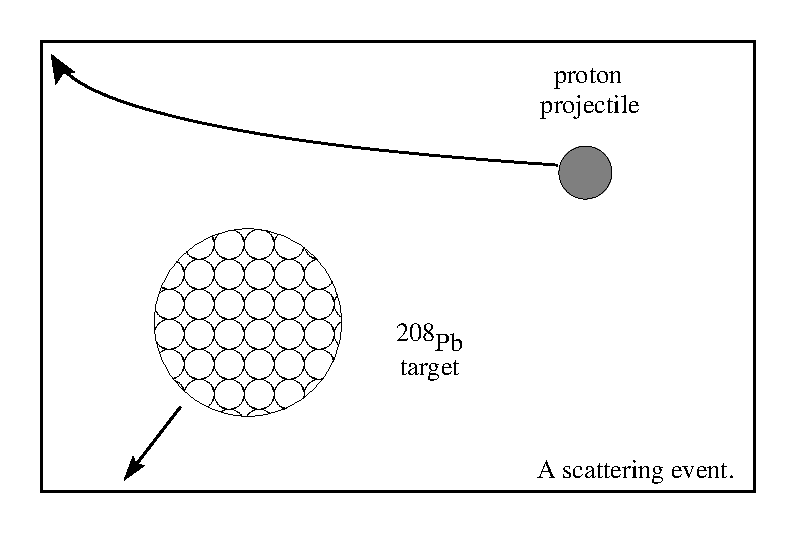
\includegraphics{electric_field_atomic_nuleus_fig_1.eps}} \par}
\vspace{0.3cm}

The final energies and velocities of the products of the reaction
are then measured and the nature of the interaction is inferred. There
are several important features of the nucleus that can be learned
from these experiments:

\begin{enumerate}
\item The nucleus is small, about 100,000 times smaller than the atom itself.
\item Most of the matter and all of the positive charge is located in this
tiny object.
\item There exists a force, called the strong force, that is attractive,
acts only within the volume of the nucleus, and is powerful enough
to overcome the repulsion between the positive charges concentrated
in the nucleus. 
\end{enumerate}
Below you will calculate the electric field of the \( ^{208} \)Pb
nucleus and the force between an incident proton and \( ^{208} \)Pb.
You will also calculate the work necessary to penetrate the nucleus.

\textbf{Activity 1: The Electric Field of \( ^{208} \)Pb}

(a) From scattering experiments like those described above one finds
that the positive charge of \( ^{208} \)Pb is uniformly distributed
throughout the volume of the nucleus, which can be treated as a sphere
of radius 7.11 x 10\( ^{-15} \) m or in units common to nuclear physics,
7.11 fm, where {}``fm'' is known as a fermi. Calculate the total
charge, Q, of the \( ^{208} \)Pb nucleus.
\vspace{30mm}

(b) Calculate the volume charge density, \( \rho  \), of the \( ^{208} \)Pb
nucleus.
\vspace{30mm}

(c) Starting with Gauss' Law, generate an expression for the electric
field, \textbf{E}, outside of the \( ^{208} \)Pb nucleus as a function
of r, the distance from the center of the sphere. Show and explain
each step of the calculation.
\vspace{2in}

(d) Use Gauss' Law to find an expression for \textbf{E} inside the
nucleus as a function of r. Show and explain each step of the calculation.
\vspace{2in}

(e) Construct a data table with the column headings r (fm), E (N/C),
and F (N) in the space below. Then use the expressions you derived
above to calculate the electric field for at least ten radial positions
between 0 and 20 fm and enter the results in the table. Include 7.11
fm as one of your radial positions.
\vspace{3in}

\textbf{Activity 2: The force on a Proton}

(a) Consider a head-on collision between a proton and the \( ^{208} \)Pb
nucleus. Generate an expression for the force on the proton as a function
of r outside the lead nucleus.
\vspace{20mm}

\vspace{1in}
(b) Calculate an expression for the force on the proton as a function
of r inside the lead nucleus.
\vspace{30mm}

(c) Use these expressions to calculate the force at the same radial
positions you calculated E and enter the results in the table.

(d) Graph F (y axis) vs. r and attach a copy to the unit.
\vspace{10mm}

\textbf{Activity 3: The Work Done by the Field}

(a) Recall that the work done by a force is \( W=\int ^{r_{f}}_{r_{i}}\overrightarrow{F}\cdot d\overrightarrow{s} \)
where r\( _{i} \) and r\( _{f} \) are the initial and final positions
of the object in motion. Treat the \( ^{208} \)Pb nucleus as a fixed
target and calculate the work done by the Coulomb force on the proton
if the proton approaches from infinity and reaches the surface of
the lead nucleus. Show all work.
\vspace{40mm}

(b) We know that the nuclear force binds particles like neutrons and
protons together once they enter the nucleus. From the graph of the
force as a function of position, what is the minimum strength of the
nuclear force in \( ^{208} \)Pb that will bind the proton in the
nucleus? Clearly state your reasoning.
\vspace{15mm}

(c) Consider a proton that has just enough initial kinetic energy
to move from infinitely far away and just reach the surface of the
lead nucleus. How is the initial kinetic energy related to the work
done by the field?
\vspace{15mm}

(d) How would the trajectory of the proton be affected if the kinetic
energy is less?
\vspace{15mm}

(e) How would the trajectory of the proton be affected if the kinetic
energy is greater?
\vspace{15mm}

(f) What minimum kinetic energy is needed for a proton to probe the
nucleus? Explain.\vspace{20mm}




\section{The Charge Distribution of the H\protect\( _{2}\protect \)O Molecule}

Name \rule{2.0in}{0.1pt}\hfill{}Section \rule{1.0in}{0.1pt}\hfill{}Date
\rule{1.0in}{0.1pt}

\textbf{Introduction}

In this exercise you will make a theoretical investigation of the
charge distribution within a water molecule (H\( _{2} \)O). The molecule
is electrically neutral and is made of 10 positive electric charges
and 10 negative electric charges (8 protons and electrons from the
oxygen atom and 1 proton and electron from each of the two hydrogen
atoms). Despite the net electrical neutrality of the molecule it can
produce an electric field if the positive and negative charges within
it have different configurations. If the most probable position of
the positive charges in the molecule does not coincide with the most
probable position of the negative charges as shown in Figure 1a, then
we call that configuration an electric dipole. Another candidate for
the charge distribution of H\( _{2} \)O is shown in Figure 1b and
is called an electric quadrupole. The most probable position of the
positive charge is either above or below the x-axis while the negative
charge is most likely to be found at the origin. This 'probabilistic'
view of the location of the charges is the basis of quantum mechanics,
the theory describing the subatomic world. Below you will calculate
the electric potential for these two charge distributions and you
will use your results to find the electric field for the dipole and
quadrupole. You will then consider the design of an experiment to
distinguish between the two different charge distributions.

\vspace{0.3cm}
{\centering 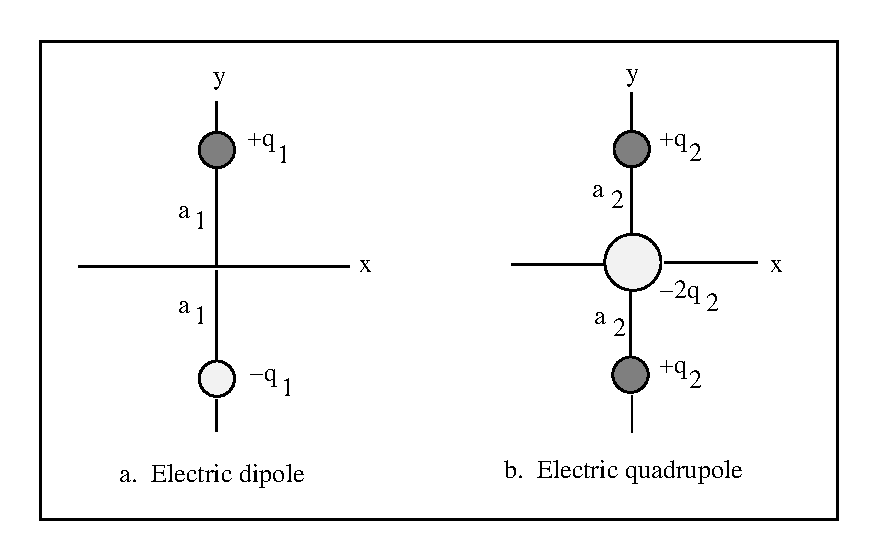
\includegraphics{charge_dist_water_mol_fig_1.eps} \par}
\vspace{0.3cm}

\textbf{Activity 1: The Electric Dipole }

(a) Calculate the electric potential, V, for the electric dipole for
a point along the y-axis, but at a position \( \left| y\right|  \)>
a\( _{1} \). Your final expression should depend on the position,
y, the charge, q\( _{1} \), and the most probable location of the
charges, a\( _{1} \).
\vspace{40mm}

(b) Generate an expression for the potential energy, U, of the charge
distribution when another charge, q\( _{test} \),  placed somewhere
on the y-axis with \( \left| y\right|  \)> a\( _{1} \).
\vspace{40mm}

(c) Recall the component of the force on a particle is related to
the potential energy of the particle by F\( _{y} \) = -\( \frac{dU}{dy} \).
Calculate the force on the test charge in terms of the position on
the y-axis, the charges, and a\( _{1} \).
\vspace{40mm}

(d) Make the approximation that the test charge is far from the molecule,
i.e., \( \left| y\right|  \) \( \gg  \) a\( _{1} \), to generate
a new expression for the force.
\vspace{40mm}

\textbf{Activity 2: The Electric Quadrupole} 

(a) Calculate the electric potential, V, for the electric quadrupole
for a point along the y-axis, but at a position \( \left| y\right|  \)
> a\( _{2} \). Your final expression should depend on the position,
y, the charge, q\( _{2} \), and the most probable location of the
charges, a\( _{2} \).
\vspace{40mm}

(b) Generate an expression for the potential energy, U, of the charge
distribution when another charge, $q_{test}$, is placed somewhere
on the y-axis with \( \left| y\right|  \) > a\( _{2} \).
\vspace{40mm}

(c) Calculate the force on the test charge in terms of the position
on the y-axis, the charges, and a\( _{2} \).
\vspace{40mm}

(d) Make the approximation that the test charge is far from the molecule,
i.e., \( \left| y\right|  \) \( \gg  \) a\( _{2} \), to generate
a new expression for the force.
\vspace{40mm}

\textbf{Activity 3: Distinguishing Between the Two Different Charge
Distributions} 

(a) Construct a table in the space below with column headings y (angstroms),
Dipole Force (arbitrary units), and Quadrupole Force (arbitrary units).
The units of distance known as angstroms are commonly used in atomic
physics. One angstrom is equal to 10\( ^{-10} \) m.
\vspace{40mm}

(b) To calculate the force on the test charge one must know the charges
and their positions for each charge distribution (q\( _{1} \), q\( _{2} \),
a\( _{1} \), a\( _{2} \)). These quantities are unknown to us at
this point. However, we want to compare the behavior of the force
due to each as a possible probe of the molecule's charge distribution.
In the expressions you generated in step (d) of Activities 1 and 2
for \( \left| y\right|  \) \( \gg  \) a\( _{1} \) or \( \left| y\right|  \)
\( \gg  \) a\( _{2} \) the forces depend on some power of y. For
\emph{convenience}, set the constant in front of this power of y to
unity. Calculate the forces for the dipole and quadrupole at distances
between 1.5 angstroms and 5.0 angstroms in 0.5 angstrom steps. Enter
your results in the table.

(c) Make a graph of the force due to the dipole and due to the quadrupole
as a function of y. Insert a copy of the graph into your notebook.

(d) In many experiments constants like those in your expressions for
the force on the test charge are unknown or poorly known. Suppose,
however, that you are able to accurately measure the radial dependence
of the force on q\( _{test} \) at distances far from the H\( _{2} \)O
molecule. If that is the case use the results from steps (b) and (c)
to propose a technique to distinguish between the two candidates for
the charge distribution of H\( _{2} \)O. Support your proposal with
a mathematical argument. (Hint: Consider a ratio involving the measured
force.)
\vspace{40mm}

(e) Experiment has found that water behaves as an electric dipole
with the electric dipole moment, q\( _{1} \)a\( _{1} \), measured
to be 6.2 x 10\( ^{-30} \) C-m. If the charge that creates the dipole,
q\( _{1} \), is the charge associated with the protons and electrons
of the molecule calculate the separation of the charges, a\( _{1} \).
How does it compare with the size of the H\( _{2} \)O molecule of
about 1.0 angstroms?\vspace{40mm}




\section{Capacitance Series Circuit}

Name \rule{2.0in}{0.1pt}\hfill{}Section \rule{1.0in}{0.1pt}\hfill{}Date
\rule{1.0in}{0.1pt}

\textbf{Objective}

\begin{itemize}
\item To investigate the relationship among charge, potential difference, and capacitance in a series combination of capacitors.
\end{itemize}
\textbf{Introduction} 

In class the series combination of capacitors was studied with the assumption
of a constant potential difference energizing the circuit.  In practice this
is difficult to reproduce in the lab because capacitors typically do not
maintain a steady charge for very long.  To get around this we will energize
the circuit with an alternating potential difference provided by a sine wave
generator.  The relationships among $Q$, $V$, and $C$ are still the same, so
we can study these circuits in the lab.

For a series combination of capacitors, the total voltage across the circuit
is the sum of the voltages across the individual capacitors, that is

\begin{displaymath} V = V_1 + V_2 + V_3 \end{displaymath}

The equivalent capacitance of the combination is given by

\begin{displaymath} \frac{1}{C} = \frac{1}{C_1} + \frac{1}{C_2} + \frac{1}{C_3} \end{displaymath}

\textbf{Apparatus}

\begin{itemize}
\item Sine wave generator 
\item Capacitors of 1.0, 4.7, and 10 $\mu$f
\item Digital multimeter
\item Connecting leads
\end{itemize}
\textbf{Activity}

%\vspace{0.3cm}
%{\centering \resizebox*{0.45\textwidth}{!}{\includegraphics{magnetism_2_fig_1.eps}} \par}
%\vspace{0.3cm}

\begin{enumerate}
\item Connect the three capacitors in series with the sine wave generator.
\item Set the sine wave generator to 200 Hz (not critical) and adjust the
amplitude so that the output measures 5 to 6 volts as measured with the
digital multimeter set for \underline{AC volts}.
\item Using the multimeter, measure $V$ for the sine wave generator and also
for each of the individual capacitors (all with uncertainties) and
list them here. Don't forget units.\vspace{20mm}
\item Calculate the total voltage and its uncertainty from the first equation
above and compare with your measured value.  Do they agree?\vspace{30mm}
\item Assuming 10 percent uncertainties on each of the capacitances,
calculate the equivalent capacitance and its uncertainty from the second
equation above.\vspace{30mm}
\item Calculate the total charge for the circuit (and its uncertainty) from
$Q = CV$.\vspace{30mm}
\item \textbf{Prediction:} How will the charge on the individual capacitors
compare with the total charge calculated above?\vspace{30mm}
\item Calculate the charge on each capacitor (and its uncertainty) and compare with the total.
Do the results agree with your prediction?
\end{enumerate}



\section{Ohm's Law}

\makelabheader %(Space for student name, etc., defined in master.tex)

\textbf{Objectives}

\begin{itemize}
\item To investigate the most important principle in electronics.
\item To determine how resistors in series and parallel add.
\end{itemize}
\textbf{Introduction}

The rate at which electric charge flows through a conductor is called
the electric current. In order to have a current, a potential difference,
or voltage is necessary. We first want to determine the relationship
between the potential difference at two ends of a conductor and the
current flowing through it.

\textbf{Note}: Do not turn on a power supply until you are sure your
circuit is correct. If you are at all unsure, please ask your instructor
to approve your setup. Ammeters can be instantly and permanently ruined
by an improper connection. Be sure to turn off the power supply before
making any changes to the circuit.

\textbf{Apparatus}

\begin{itemize}
\item Power supply
\item Two resistors
\item Leads and alligator clips
\item DC Milliammeter
\item Multimeter
\end{itemize}
\textbf{Activity 1: Ohm's Law}

\begin{itemize}
%\item Connect two rheostats (or variable resistors) in series as shown in
%the figure below. Set R\( _{1} \) at about the halfway point and
%R\( _{2} \) at the maximum. Connect an ammeter as shown. Also, connect
%a voltmeter across (that is, connect a probe to each side of) R\( _{1} \).
%\item The fixed resistor will be considered an ``unknown'' and will be called 
%R\( _{1} \). The variable resistor will be called R\( _{2} \), and will be used 
%to vary the current. Connect the two resistors in series as shown in the 
%figure. Set R\( _{2} \) at its maximum value. Connect a milliammeter as shown, 
%at the point marked ``A'' (for ``ammeter''). Leave the positive lead to the 
%power supply disconnected.
\item With the power supply off, turn the coarse current control all the way up 
and both voltage controls all the way down.  Connect one of the resistors in 
series with the milliammeter (marked ``A'' for ``ammeter'') as shown in the 
figure below. Be sure the polarity of the milliammeter is as shown.
\end{itemize}
\vspace{0.3cm}
{\centering \resizebox*{0.35\textwidth}{!}{\includegraphics{ohms_law/ohms_law_fig_3.eps}} \par}
\vspace{0.3cm}

\begin{itemize}
\item When sure of your circuit, turn on the power supply, and turn the coarse 
voltage control up until the milliammeter reads 20 ma. Measure the voltage 
across the resistor (with the multimeter set for DC voltage) and record both voltage and current here. Include an uncertainty in the voltage measurement.
\vspace{10mm}

%\item Reduce the resistance of R\( _{2} \) and record the current and voltage
%three more times by turning down R\( _{2} \) in approximately equal steps so 
%that for the last time R\( _{2} \) is turned completely down. 
%Record your results here:\vspace{30mm}

\item Now turn the coarse voltage control up and record current and voltage 
for four more values of current: 40, 60, 80, and 100 ma. Include uncertainties
 in the voltage measurements.
\vspace{30mm}

\item Turn off the power supply.

\item Using $Excel$, plot your five pairs of readings with the voltage on the 
vertical axis and the current on the horizontal axis. Include the origin as a 
sixth point (why is this valid?).
\vspace{6mm}
\item Fit a straight line to the points (including the origin).
Include a trendline with equation.
\item Use the LINEST function in $Excel$ (see \textbf{Appendix C}) to 
determine the slope of the line and its uncertainty.  What is the meaning 
of the slope? Write its value with uncertainty here (including units):
\vspace{20mm}

\item Print the graph and include it with this unit.

\item Remove the resistor from the rest of the circuit and use the ohmmeter
option on the multimeter to measure the resistance of R directly.
Does it fall within the range of values determined above? Can you think of 
a reason for any discrepancy?
\vspace{20mm}

\item What is the general relationship between voltage, current, and resistance?
This is Ohm's Law.\vspace{15mm}

\item Why is the origin a legitimate point on the curve?\vspace{15mm}

\end{itemize}
\textbf{Activity 2: Resistors in Series}

\begin{itemize}
%\item Turn rheostat R\( _{2} \) to its maximum setting. Connect the multimeter
%across this resistor, being sure to set it for reading voltages.
%\item When you are sure the circuit is set, turn on the power supply and
%record the current and voltage. Turn off the power supply.\vspace{10mm}

%\item \textbf{Prediction}: Based on your measurements, predict the resistance
%of R\( _{2} \).\vspace{15mm}

%\item Remove and measure the resistance of R\( _{2} \). Record the percent
%difference between your prediction and measurement. Replace R\( _{2} \).\vspace{30mm}

%\item Was the current this time different from the first reading in Activity
%1?\vspace{15mm}

\item Turn the voltage control down to zero, and connect two resistors in 
series as shown in the figure below.
\end{itemize}
\vspace{0.3cm}
{\centering \resizebox*{0.35\textwidth}{!}{\includegraphics{ohms_law/ohms_law_fig_1.eps}} \par}
\vspace{0.3cm}

\begin{itemize}

\item Turn on the power supply and turn up the coarse voltage control to 
approximately 10 volts. Measure the voltages across R\( _{1} \), R\( _{2} \), 
and the milliammeter. (The voltage across the milliammeter may be in \underline{millivolts}.) Also measure the total voltage across all three elements 
in series. Include uncertainties in each measurement. Record your results here:
\vspace{20mm}

\item How is the last measurement related to the three individual 
measurements?
\vspace{10mm}

\item What can you conclude about the voltage across resistors in series?
\vspace{10mm}

\item Measure the current in the series circuit and record it here:
\vspace{10mm}

\item Using Ohm's Law, determine the total resistance of the circuit from the 
total voltage and the current which you have measured.
\vspace{10mm}

%\item Connect the multimeter across both resistors, being sure to switch
%to voltage readout.
%\item When you are sure the circuit is correct, turn on the power supply
%and record the current and voltage. Turn off the power supply.\vspace{10mm}

%\item Has the current changed?\vspace{15mm}

%\item Has your previous conclusion been substantiated or refuted?\vspace{15mm}

%\item How is the voltage just measured related to the first voltage measurements
%in Activities 1 and 2?\vspace{15mm}

%\item What can you conclude about the voltage across resistors in series?\vspace{15mm}

\item Turn the voltage control down to zero and turn off the power supply.

\item Calculate R\( _{1} \), R\( _{2} \), and R\( _{A} \) from Ohm's Law and 
your above readings. From these three values, determine the total resistance of 
the circuit. Does it agree with the value you calculated above? Record your 
results here:
\vspace{20mm}

\item What can you conclude about the total resistance in a circuit 
containing resistors in series?\vspace{15mm}

\end{itemize}

\pagebreak

\textbf{Activity 3: Resistors in Parallel}

\begin{itemize}
\item Connect the two resistors in parallel as shown in figure \textbf{a} 
below, with the milliammeter at the point marked ``A''. Have circuit checked 
before continuing.
\end{itemize}
\vspace{0.3cm}
\begin{center}
%\includegraphics[width=6.0in]{ohms_law_fig_2.eps}
\includegraphics[width=4.6in]{ohms_law/ohms_law_fig_2b.eps}
\end{center}
\vspace{0.3cm}

\begin{itemize}
\item When you are sure the circuit is set up correctly, turn on the power 
supply and turn the coarse voltage control up to about 10 volts. Record the 
total current through the circuit and the voltage across 
the parallel resistance combination. Also measure the voltage across the 
milliammeter (which may be in millivolts). Turn off the power supply.
\vspace{20mm}

\item Connect the milliammeter to the point marked A\( _{1} \) in figure 
\textbf{b} above, without disturbing the rest of the circuit. Turn on the 
 power supply and 
record the current through R\( _{1} \) and the voltage across the parallel 
combination. Turn off the power supply.
\vspace{20mm}

\item Repeat the above measurements for R\( _{2} \), connecting the 
milliammeter at A\( _{2} \) as in figure \textbf{c} above. Turn off the 
power supply.
\vspace{20mm}

%\item Using Ohm's Law, calculate the two resistances of the parallel connection
%and also the total resistance of the circuit. Check with the ohmmeter
%and determine the percent differences.\vspace{30mm}

\item What is the relationship between the total current and the current
in each of the branches of the parallel circuit? (This is an example of 
Kirchhoff's junction rule which is based on conservation of charge.)
\vspace{30mm}

\item Using Ohm's Law and your data above, calculate the resistance of each 
resistor and the total resistance of the circuit.
\vspace{60mm}

\item What is the relationship between the total resistance of the parallel
circuit and the resistance of each of the branches? Using this relationship, 
calculate the total resistance of the circuit from the individual resistances 
you determined above. Does the result agree with what you calculated in the 
previous item? Calculate a percent difference and record it here.


%\item Determine, using Ohm's law, what the voltage was in each branch of
%the parallel circuit. Did it make any difference that you didn't reposition
%the voltmeter during this activity? On the basis of Ohm's law, does
%the result make sense?\vspace{30mm}

%\item Can the total resistance of a series combination ever be less than
%the resistance of the largest resistor? Explain.\vspace{30mm}

%\item Can the total resistance of a parallel combination ever be greater
%than the resistance of the smallest resistor? Explain.\vspace{30mm}
\end{itemize}




\section{Kirchhoff's Rules}

Name \rule{2.0in}{0.1pt}\hfill{}Section \rule{1.0in}{0.1pt}\hfill{}Date
\rule{1.0in}{0.1pt}

\textbf{Objective}

\begin{itemize}
\item To study Kirchhoff's rules for analyzing circuits.
\end{itemize}
\textbf{Introduction}

Two statements comprise Kirchhoff's rules. The first, the so-called
junction rule, restates the conservation of charge; the second, the
so-called loop rule, restates the conservation of energy:

\begin{enumerate}
\item The sum of the currents entering any junction (or node) must equal
the sum of the currents leaving that junction.
\item The algebraic sum of electrical potential changes across all the elements
around any closed loop must be zero.
\end{enumerate}
\textbf{Note}: Do not turn on a power supply until you are sure your
circuit is correct. Please ask your instructor to approve your setup.
Ammeters can be instantly and permanently ruined by an improper connection.
Be sure to turn off the power supply before making any changes to
the circuit.

\textbf{Apparatus}

\begin{itemize}
\item power supply
\item three-resistor board
\item analog ammeter
\item digital voltmeter
\end{itemize}
\textbf{Activity}

\vspace{0.3cm}
{\centering \resizebox*{0.5\textwidth}{!}{\includegraphics{kirchhoffs_rules/kirchhoffs_rules_fig_1.eps}} \par}
\vspace{0.3cm}

\begin{enumerate}
\item Referring to the circuit above, choose a junction and write an equation
which satisfies Kirchhoff's first rule.\vspace{20mm}

\item Identify two closed loops on the circuit which contain at least one
element not included in the other. Write an equation for each loop
that satisfies Kirchhoff's second rule.\vspace{20mm}

\item You now have three equations that can be solved for the three currents
in terms of the supplied voltage (emf), \( \varepsilon  \), and the
three resistors, R\( _{A} \), R\( _{B} \), and R\( _{C} \). Carry
out the algebra to obtain expressions for the three currents in terms
of these quantities.\vspace{50mm}

\item Now use Ohm's law and the sum rules for resistors in series and in
parallel to derive expressions for the three currents.\vspace{50mm}

\item Are the results of 3 and 4 the same? They should be.\vspace{15mm}

\item Set a digital multimeter to measure resistance. Determine and record
values for the three resistors, R\( _{A} \), R\( _{B} \), and R\( _{C} \),
which are mounted on the wooden block.\vspace{15mm}

\item \textbf{Prediction}: if the emf, \( \varepsilon  \), were 5.0 V,
what do you predict the three currents would be?\vspace{30mm}

\item Configure the circuit as in the figure above, using the power supply
as the source of emf. With the power supply off, set the current control
at mid-range and the voltage control all the way down. Set the digital
multimeter to measure voltage and connect it in parallel with the
power supply to measure \( \varepsilon  \). Connect the analog ammeter
in series with resister R\( _{A} \) to measure the current I\( _{A} \).
\item After checking with your instructor that the circuit is correct, turn
on the power supply and set \( \varepsilon  \) to about 5.0 V. Record \( \varepsilon  \) and I\( _{A} \), then turn off the power supply.\vspace{15mm}

\item Set up the circuit to measure I\( _{B} \). After getting assurance
from you instructor that your circuit is correct, turn on the power
supply and record \( \varepsilon  \) and I\( _{B} \). Turn off the
power supply.\vspace{15mm}

\item Set up, measure and record I\( _{C} \).\vspace{15mm}

\item Do your results agree with your prediction? How large, in terms of
percentage, are the discrepancies? Speculate on what might cause any
differences.\vspace{15mm}
\end{enumerate}



\setcounter{equation}{0}

\section{RC Circuits}

\makelabheader %(Space for student name, etc., defined in master.tex)

\textbf{Objective}

\begin{itemize}
\item To investigate the behavior of a series RC circuit, i.e. one containing a resistor and a capacitor in series with a DC power supply of fixed emf $V_{0}$.
\end{itemize}
\textbf{Introduction} 

For the charging circuit, the charge on the capacitor as a function of time
is given by
\begin{equation}
Q(t)=CV_{0}\left(1-e^{-t/RC}\right)
\end{equation}
while for the discharging circuit (no emf) the charge is
\begin{equation}
Q(t)=Q_{0}e^{-t/RC}
\end{equation}
where $Q_{0}$ is the initial charge on the capacitor.  Since $Q=CV$ for the
capacitor, the voltage across the capacitor has the same time dependence,
namely
\begin{equation}
V(t)=V_{0}\left(1-e^{-t/RC}\right)
\end{equation}
for the charging circuit and
\begin{equation}
V(t)=V_{0}e^{-t/RC}
\end{equation}
for the discharging circuit.
\vspace{5mm}

We will use the discharging circuit in this experiment.
For this circuit, the time required for $Q$ (or $V$) to decrease to
$1/e$ of its initial value (the time constant) is
\begin{equation}
\tau=RC
\end{equation}
The time required for $Q$ (or $V$) to decrease to 1/2 of its initial value (the
half-life) is
\begin{equation}
t_{1/2}=(ln2)\tau =.693\tau
\end{equation}
This will be useful because in practice it is easier to measure the half-life
than the time constant.


\textbf{Apparatus}

\begin{itemize}
\item DC power supply (low voltage)
\item Electrolytic capacitor (1000-5000 $\mu$f)
\item Voltmeter (0-3V)
\item Stop watch
\item Connecting leads
\item Voltage sensor
\end{itemize}
\textbf{Activity 1: Proof of Equation (6)}

Prove equation (6) above, beginning with equation (2).
\vspace{3in}

\textbf{Activity 2: Measurement of Half-life}

The capacitor will be charged briefly, then allowed to discharge through the
voltmeter which will act as the resistor in this case. The internal resistance
of the voltmeter (0-3V) is about 3000 ohms.  Assume this is known to within
10\% and the capacitance as marked is known to within 10\%.

\begin{enumerate}
\item Connect the voltmeter directly across the capacitor.  Electrolytic
capacitors are polarity sensitive, so be sure the terminal marked with a minus
sign is connected to the \underline{negative} terminal of the voltmeter.

\item Set the power supply to about 2.5 volts and connect its negative terminal
to the negative terminal of the capacitor.

\item Connect the positive terminal of the power supply to the corresponding
terminal of the capacitor briefly to charge it, then disconnect the positive 
lead and observe the exponential decay of the voltage.  Use a stop watch to 
measure the half-life (5 trials) as follows: switch the stop watch on when the 
voltmeter reads 2.0 volts, and switch it off when the meter reads 1.0 volt. 
Record your five measurements here.\vspace{30mm}

\end{enumerate}

\textbf{Activity 3: Determination of Time Constant}

\begin{enumerate}
\item Experimental:  Find the average of your five half-life measurements and 
its uncertainty (the standard deviation) and determine the time constant from 
equation (6) above, and its uncertainty. (Note: Since the time constant and the 
half-life are directly proportional, the fractional uncertainty in the time 
constant will be the same as the fractional uncertainty in the half-life.)
\vspace{40mm}
\item Theoretical:  Calculate the time constant and its uncertainty from 
equation (5). Do your two results agree within experimental uncertainties?
\end{enumerate}

\newpage

\textbf{Activity 4: Determination of Time Constant Using Pasco Interface and Computer}

We will now look at a graph of the discharge curve using the Pasco interface 
and computer. Plug the voltage sensor into the input channel $A$ of the Pasco 
interface. Then connect the red and black leads from the voltage sensor to the 
terminals of the capacitor (the voltmeter should still be connected to the 
capacitor as before), being sure to connect the red lead to positive and black 
lead to negative. Connect the negative lead from the power supply to the 
negative terminal of the capacitor.
\vspace{10mm}

To record voltage versus time data, go to $Start$ $\rightarrow$ $Programs$ 
$\rightarrow$ $Physics Applications$ $\rightarrow$ $Data Studio$. Select the 
option $Create Experiment$. You will see an image of the 750 interface box. 
On this image, single click on the channel $A$ input. You will see a list of 
sensors. Scroll down to the $voltage sensor$ and select by clicking $OK$. 
Finally, open a graph display by double clicking on the $Graph$ option (on 
the left).
\vspace{10mm}

Make sure your power supply is still set at around 2.5 volts. Charge the 
capacitor (by touching the positive lead from the power supply to the positive 
capacitor terminal) and click the $Start$ button to begin taking data. 
Disconnect the positive power supply lead and you will see the 
discharge curve on the screen as the capacitor discharges. When you have an 
acceptable curve, click $Stop$. Print the graph and attach it to this unit.
\vspace{10mm}

Use the $Smart$ tool to determine the time when the voltage is 2.00 volts 
and again when the voltage is 1.00 volt. The difference is the half-life. 
Record it here, with an \underline{estimated} uncertainty:
\vspace{40mm}

Now calculate the time constant and its uncertainty from equation (6) and 
compare with your value of $RC$ determined from equation (5). Do they agree 
within experimental uncertainty (i.e. do the ranges overlap)?




\section{Magnetism I}

Name \rule{2.0in}{0.1pt}\hfill{}Section \rule{1.0in}{0.1pt}\hfill{}Date
\rule{1.0in}{0.1pt}

\textbf{Objectives}

\begin{itemize}
\item To investigate the characteristics of magnets.
\item To understand how a compass works.
\end{itemize}
\textbf{Introduction} 

The electric interaction, you probably know, is not the only one in
which opposites attract and likes repel. Magnetic interactions have
similar characteristics. All simple magnets, regardless of size, are
bipolar: there are two magnetic poles. Consider this question, then:
Can we talk about like and unlike as we do for electricity?

\textbf{Apparatus}

\begin{itemize}
\item 2 bar magnets 
\item 2 cylindrical magnets 
\item rods and clamps
\item wool cloth
\item rubber rod
\item string
\end{itemize}
\textbf{Activity 1: The Characteristics of Magnets}

\begin{enumerate}
\item Feel the attraction between two magnets when pulled apart after having
come together without effort on your part. Describe qualitatively
in terms of strength and separation.\vspace{15mm}

\item Feel the repulsion when one of them is turned around and pushed toward
the other. Describe as in step 1.\vspace{15mm}

\item Note and describe the difference in (strength and direction of) interactions
between the ends and the middle.\vspace{15mm}

\end{enumerate}
\textbf{Activity 2: How a Compass Works}

\begin{enumerate}
\item Identify geographic north and south.
\item Hang one of the cylindrical magnets horizontally from a horizontal rod.
\item When it comes to rest, along which geographical line does the magnet
lie? \vspace{15mm}

\item Which end (colored or uncolored) is the \char`\"{}north-seeking\char`\"{}
end?\vspace{15mm}

\item Remove the cylindrical magnet and repeat step 2 with the second cylindrical magnet. Answer, again, the questions above.\vspace{15mm}

\item What happens when you bring the \char`\"{}north-seeking\char`\"{}
end of the first magnet near the hanging one's north-seeking end?\vspace{15mm}

\item What happens when you bring the first magnet's opposite end near the
second's north-seeking end?\vspace{15mm}

\item What about the first magnet's north-seeking end near the opposite
end of the hanging one?\vspace{15mm}

\item What happens when you bring the opposite ends near one another?\vspace{15mm}

\item Define in your own words like and unlike poles?\vspace{15mm}

\item What always happens between like poles?\vspace{15mm}

\item What always happens between unlike poles?\vspace{15mm}

\item Determine with a labelled bar magnet which end of your hanging magnet
should be identified as the north pole and which the south.
\vspace{10mm}
\item Why do we identify one end of a magnet as the north pole and the other
as the south?\vspace{15mm}

\item In your own words, explain a compass.\vspace{15mm}

\item In terms of magnetism, what is the earth?\vspace{15mm}

\item Charge a rubber rod with the wool cloth and bring it near the ends
of the suspended magnet; describe its effect on the magnet.\vspace{15mm}

\item Does a south magnetic pole repel a negative electric charge?\vspace{15mm}

\item Does a north magnetic pole attract a negative electric charge?\vspace{15mm}
\end{enumerate}




\section{Magnetism II}

Name \rule{2.0in}{0.1pt}\hfill{}Section \rule{1.0in}{0.1pt}\hfill{}Date
\rule{1.0in}{0.1pt}

\textbf{Objective}

\begin{itemize}
\item To investigate the magnetic field around a permanent magnet.
\end{itemize}
\textbf{Introduction} 

The magnetic field characterizes magnetic forces in much the same way
that the electric field characterizes electric forces.
At a given point in the region around a magnet,,
the strength of the field, similar to that of an electric field, is
the force per unit north pole (one positive unit of magnetism), and
the direction is indicated by the orientation of the north pole of
a compass located at the point. On earth, the field mapped out around
the magnet is actually the resultant of the field due to the magnet
and the field due to the earth.

\textbf{Apparatus}

\begin{itemize}
\item 2 bar magnets 
\item small compass 
\item white paper and tape
\end{itemize}
\textbf{Activity 1: A Single Bar Magnet}

\vspace{0.3cm}
{\centering \resizebox*{0.45\textwidth}{!}{\includegraphics{magnetism_2_fig_1.eps}} \par}
\vspace{0.3cm}

\begin{enumerate}
\item Center and tape a bar magnet on a piece of paper and orient it so
that the magnet's south pole points to the earth's geographic north
pole. Indicate the magnet's polarity and the direction of the earth's
field.
\item Place the small compass near the north pole of the magnet and make
a dot at each end of the needle using a pencil not encased in metal.
\item Move the compass forward until its south pole points at the previous
north pole dot, and make a new dot at the north pole.
\item Repeat 3 until the series of dots reaches the south pole of the magnet
or the edge of the paper.
\item In a similar manner, trace enough lines to map the magnetic field
over the entire paper. Take points about 0.5 cm apart near the poles
and about 2 cm apart near the middle of the magnet.
\item There are two points, called neutral points, near each end of the
magnet where the magnet's field and the earth's field are equal and
opposite and so cancel. At these points, the compass will align in
no particular direction. Try to locate these points by tracing very
carefully the lines of force in the neighborhood of the poles.
\item Do lines of force ever cross?\vspace{15mm}

\item Where are the magnetic forces strongest? Weakest? How do the force
lines indicate this? Does a line of force represent a constant force
along its entire length?\vspace{15mm}

\item Do the lines intersect the magnet at a particular angle (like the
electric field lines near a conductor)? What does this imply about
the source of a magnetic field as opposed to the surface charge of
a conductor as the source of an electric field? \vspace{15mm}

\end{enumerate}
\textbf{Activity 2: Two Bar Magnets--Unlike Poles Facing One Another}

\vspace{0.3cm}
{\centering \resizebox*{0.45\textwidth}{!}{\includegraphics{magnetism_2_fig_2.eps}} \par}
\vspace{0.3cm}

\begin{enumerate}
\item Set up two bar magnets on a sheet of paper as shown in the figure
above. The magnets should be 8-10 cm apart.
\item Repeat steps 2 through 5 from the previous activity.
\item What sort of charge configuration produces an electric field that
looks similar to the magnetic field you just identified?\vspace{15mm}

\item What differences can you recognize?\vspace{15mm}

\end{enumerate}
\vspace{25mm}
\textbf{Activity 3: Two Bar Magnets--Like Poles Facing One Another}

\vspace{0.3cm}
{\centering \resizebox*{0.45\textwidth}{!}{\includegraphics{magnetism_2_fig_3.eps}} \par}
\vspace{0.3cm}

\begin{enumerate}
\item Set up two bar magnets on a sheet of paper as shown in the figure
above. The magnets should be 8-10 cm apart.
\item Repeat steps 2 through 5 from Activity 1 of this investigation.
\item Try to identify on your map a point at which the magnetic field is
zero. Explain what causes this effect.\vspace{15mm}

\item What sort of electric charge configuration would produce a similar
field map?\vspace{15mm}
\end{enumerate}




\section{Magnetism III}

Name \rule{2.0in}{0.1pt}\hfill{}Section \rule{1.0in}{0.1pt}\hfill{}Date
\rule{1.0in}{0.1pt}

\textbf{Objectives}

To investigate:

\begin{itemize}
\item The effect of magnetic fields on moving charges. 
\item The effect of moving charges (currents) on magnets. 
\end{itemize}

\textbf{Apparatus} 

\begin{itemize} 
\item Bar magnet
\item Oscilloscope
\item Tangent galvanometer
\item Compass
\item Power supply
\item Banana plug leads (2) with alligator clips
\end{itemize}

%\textbf{Introduction} 

%Where did this intro come from??? It has nothing to do with the lab!
%A charged object moving through a magnetic field experiences a force
%which is proportional to the magnitude of its charge and to its speed
%perpendicular to the field: $F = qvB_\perp$. Changing the number of
%magnetic field lines--the flux--through a coil of wire results in
%a current in the wire. The direction of this current is such that
%the magnetic field it produces opposes the change in the external
%field. Similarly, varying the current in one coil (the primary) produces
%a current in another nearby coil (the secondary). The current in the
%second coil, too, will flow in a direction that creates a magnetic
%field opposing that which is changing in the first coil. These relationships
%between changing fields and currents are known collectively as electromagnetic
%induction.



\textbf{Activity 1: Magnetic Forces on Moving Charges }

\begin{enumerate}
\item An oscilloscope is built around the principle of the cathode ray tube. It emits electrons from its back end. These are accelerated by a series of electrodes and focused to strike a fluorescent screen at its front. The result is a visible spot (or trace) indicating voltage as a function of time.

\item \textbf{Predictions}: What, if anything, will happen to the spot on
the screen if the north pole of a magnet is brought near the left
side of the oscilloscope? What will happen if you do the same with
the south pole? What about when each of the poles are brought near
to the top? {[}Please do not touch the oscilloscope with the magnet.{]} 
\vspace{30mm}

\item Turn on the oscilloscope by pressing the power button. Turn the TIME/DIV 
knob completely counterclockwise. Adjust the INTEN (intensity) and FOCUS knobs 
so that a small bright spot is formed on the oscilloscope screen by the beam of 
electrons traveling toward the screen. Do not make the spot very bright. 
Adjust the ILLUM (illumination) knob so that the grid on the screen can be seen 
clearly. Use the horizontal and vertical POSITION controls to center the spot 
on the screen.

\item Bring the N-pole of a horizontal bar magnet near, but not touching,
the left side of the oscilloscope case at the height of the spot.
Record the direction of any deflection. Repeat with the S-pole.\vspace{20mm}

\item Bring the N-pole of a vertical bar magnet near, but not touching,
the top of the oscilloscope case just above the spot. Record the direction
of any deflection. Repeat with the S-pole.\vspace{25mm}

\item Turn off the oscilloscope.
\item Did the directions of deflections meet your expectations? Explain. 
\vspace{25mm}

\end{enumerate}

\textbf{Activity 2: The Effect of Moving Charges (Currents) on Magnets}

In this investigation we will use a device known as a tangent galvanometer to make a qualitative study of the effect of current (moving charges) in a coil of wire on a compass. A sketch of the galvanometer is shown below.

\begin{center}
\includegraphics{magnetism_3/tangent_galvanometer.eps}
\par
Figure 1. Tangent galvanometer and compass.
\end{center}

\begin{enumerate}

\item With the power supply off, connect the positive and negative terminals 
on the power supply to the two side screws on the tangent galvanometer. Turn 
the coarse current control on the power supply all the way up and the voltage 
controls all the way down.

\item Before turning the power supply on, place the compass on the platform 
in the center of the tangent galvanometer. Rotate the galvanometer until the 
compass needle is aligned with the plane of the wire coil of the galvanometer.
Turn the power supply on and slowly turn up the fine voltage control.
What do you observe? Make a sketch to show the orientation of the compass 
needle and galvanometer coil with the voltage on and off. 
(It may be easiest to do this with TOP views.)
\vspace{20mm}

\newpage

\item Turn the voltage on the power supply to zero.
Rotate the entire setup (galvanometer, compass, wires) $180^\circ$
so the contacts are on the opposite side from where they were before.
Make sure the compass needle is again aligned with the plane of the wire coil.
Slowly turn the voltage back up. What do you observe?
Make another sketch to show the orientation of the compass needle and
galvanometer coil with the voltage on and off.
\vspace{30mm}

\item The deflection of the compass when current flows in the tangent 
galvanometer implies the current creates a magnetic field.
From your observations can you tell the direction
of the magnetic field?  Explain.
\vspace{30mm}

\item Reverse the wires on the contacts of the tangent galvanometer to reverse 
the direction of the current in the coil of the galvanometer.
We will now repeat the observations from above.
With the voltage off, align the compass needle and the plane of the wire coil 
of the galvanometer as in number 2 above.
Slowly turn up the voltage.
What do you observe?
Make a sketch to show the orientation of the compass and
galvanometer coil with the voltage on and off.
\vspace{30mm}

\item Rotate the entire setup (galvanometer, compass, wires) $180^\circ$
so the contacts are on the opposite side from where they were before.
Make sure the compass needle is again aligned with the plane of the wire coil.
Slowly turn the voltage back up. What do you observe?
 Make another sketch.
\vspace{30mm}

\item Based on your observations, what happens to the magnetic field of the 
tangent galvanometer when you reverse the direction of the current?

\end{enumerate}


\setcounter{equation}{0}

\section{Magnetic Field of the Earth}

\makelabheader %(Space for student name, etc., defined in master.tex)

\textbf{Objective}

\begin{itemize}
\item A measurement of the earth's magnetic field.
\end{itemize}
\textbf{Introduction} 

The magnetic field lines of a bar magnet, though emanating from its
full length, are densest near the poles. These lines are typically
not perpendicular to the faces of the magnet. The Earth, as you know,
is like a giant bar magnet, with its magnetic south pole near its
geographic north pole.

The field lines of the Earth's magnetic field, therefore, tend to
point obliquely at any given spot on its surface. The angle (let's
call it \( \phi  \)) that a line makes with a surface is known as
its \emph{dip angle} (see figure). Thus, each locality on earth has
its characteristic value for \( \phi  \) with regard to the terrestrial
magnetic field.

\begin{center} \begin{picture}(200,70) \put(0,0){\line(1,0){200}} \put(150,50){\vector(-2,-1){100}} \put(150,50){\vector(0,-1){50}} \put(150,50){\vector(-1,0){100}} \put(100,60){\makebox(0,0){$B_h$}} \put(160,25){\makebox(0,0){$B_v$}} \put(90,30){\makebox(0,0){$\bf B$}} \put(75,6){\makebox(0,0){$\phi$}} \put(60,0){\oval(10,10)[tr]} \end{picture} \end{center}

The horizontal component of the Earth's magnetic field,

\begin{equation}
B_h = B\cos\phi,
\end{equation}

causes the magnetized needle of a compass to align in the geographic
north-south direction.

%%This is about 1000 times more complicated than it has to be!
% by producing a torque on it. Recall that the
%magnitude of a torque is \( \tau  \) = r F\( \sin \theta  \), where
%F is the force, r is the distance from the axis of rotation to the
%point at which the force acts, and \( \theta  \) is the angle between
%the line from the axis of rotation to the point of interaction and
%the direction of the force.
%
%\begin{center} \begin{picture}(200,75) \put(0,0){\line(0,1){10}} \put(150,0){\line(0,1){10}} \put(65,5){\vector(-1,0){65}} \put(85,5){\vector(1,0){65}} \put(75,5){\makebox(0,0){$\bf r$}} \put(0,15){\circle*{3}} \put(80,55){\makebox(0,0){$\tau = r F \sin\theta$}} \put(150,15){\vector(0,1){50}} \put(150,15){\vector(3,4){37.5}} \put(160,20){\makebox(0,0){$\theta$}} \put(130,35){\makebox(0,0){$F \sin\theta$}} \put(170,50){\makebox(0,0){$\bf F$}} \thicklines \put(0,15){\line(1,0){200}} \end{picture} \end{center}
%
%The force on the compass is due to the Earth's magnetic field,
%F = pB, where p is the so-called \emph{pole strength} (recall that
%F = qE, for static electric fields, where q is the charge). In this
%case, the force acts on both ends of the magnet, so that r (the distance
%from the axis of rotation to the point at which the force acts) is
%half the length of the compass needle, $l$; \( \theta  \) is the
%angle between the alignment of the compass needle and the direction
%of B\( _{h} \). Hence, the torque on a compass needle due to the
%Earth's magnetic field is
%
%\begin{displaymath} \tau_e = plB_h\sin\theta. \end{displaymath}
%

You will use a tangent galvanometer to produce an additional horizontal
magnetic
field perpendicular to the Earth's field (in other words, one that
points east or west).
A tangent galvanometer consists of a vertical, circular coil of wire
with N turns, a pedestal compass at the center of the coil, and electrical
contacts so that a direct current can be established in the coil.
The magnetic field at the center of the galvanometer coil caused by a current
I in the coil is

\begin{equation}
B_c = N\frac{\mu_0I}{2R}
\end{equation}

where R is the radius of the coil and \( \mu _{0} \) is the permeability
of free space (1.25664 x 10\( ^{-6} \) T\( \cdot  \)m/A). B\( _{c} \)
is perpendicular to the vertical plane of the coil. If the plane of
the coil is placed in the north-south direction (that is, parallel
to the compass needle when there is no current in the coil), then,
when there is current in the coil, the compass will be influenced
by two perpendicular fields, B\( _{h} \) and B\( _{c} \). 
The compass needle will now point in the direction of the vector
sum ${\bf B}_h+{\bf B}_c$.  

Let $\theta$ be the angle through which the compass needle turns
when the current in the tangent galvanometer is turned on.
In other words, $\theta$ is the angle between ${\bf B}_h$ and
${\bf B}_h+{\bf B}_c$.  Sketch a picture of these vectors, and
use it to convince yourself that

%The
%latter provides a second torque (see figure, checking carefully the
%angles, \( \cos \theta =\sin (\frac{\pi }{2}-\theta ) \) ):
%
%\begin{displaymath} \tau_c = plB_c\cos\theta \end{displaymath}
%
%\begin{center} \begin{picture}(150,150) \put(10,75){\line(1,0){100}} \put(60,25){\line(0,1){100}} \put(5,75){\makebox(0,0){W}} \put(60,130){\makebox(0,0){N}} \put(115,75){\makebox(0,0){E}} \put(60,20){\makebox(0,0){S}} \put(34,40){\vector(3,4){54}} \put(34,40){\vector(-1,0){10}} \put(34,40){\vector(0,-1){10}} \put(88,112){\vector(1,0){10}} \put(88,112){\vector(0,1){10}} \put(65,90){\makebox(0,0){$\theta$}} \multiput(34,40)(12,-9){4}{\line(4,-3){10}} \multiput(88,112)(12,-9){4}{\line(4,-3){10}} \multiput(60,75)(12,-9){2}{\line(4,-3){10}} \put(15,40){\makebox(0,0){$\scriptstyle pB_c$}} \put(108,112){\makebox(0,0){$\scriptstyle pB_c$}} \put(34,25){\makebox(0,0){$\scriptstyle pB_h$}} \put(88,127){\makebox(0,0){$\scriptstyle pB_h$}} \put(92,81){\makebox(0,0){$\scriptstyle r$}} \put(104.5,43){\makebox(0,0){$\scriptstyle l$}} \put(89,77){\vector(-3,-4){10}} \put(95,85){\vector(3,4){10}} \put(100,37){\vector(-3,-4){20}} \put(109,49){\vector(3,4){20}} \end{picture} \end{center}
%
%When current is established in the coil, the needle will rotate through
%an angle \( \theta  \) with respect to the plane of the coil until
%the opposing torques are equal in magnitude. Thus, when equilibrium
%is established, we have
%
%\begin{displaymath} \tau_e = \tau_c \Rightarrow plB_h\sin\theta = plB_c\cos\theta \end{displaymath}

\begin{equation}
%\begin{displaymath} 
B_h = \frac{B_c}{\tan\theta} 
%\end{displaymath}
\end{equation}

\vskip 1in

By measuring the angle $\theta$, we can determine $B_h$.  
If we then measure the dip angle $\phi$, we can determine
the Earth's magnetic field from equation (1) above.

\textbf{Apparatus}

\begin{itemize}
\item tangent galvanometer 
\item power supply 
\item DC ammeter (0-1 amp)
\item banana plug leads (1 red, 2 black) with alligator clips
%\item switch
\item compass
\item ruler 
\item dip angle compass 
%\item wooden stand
\end{itemize}
\vspace{15mm}
\textbf{Activity}

\begin{enumerate}
\item Measure and record on the accompanying data sheet the diameter D of
the galvanometer coil. Calculate and record the radius R of the coil.
\item Count and record the number of turns, N, of the coil.
\item With the power supply off, connect its positive and negative terminals 
to the tangent galvanometer and  a DC ammeter (in series). 
Be sure the ammeter is connected in \underline{series} with 
the coil. Use long wires to connect the outside terminals of the coil
to the circuit so that the coil may be removed from the magnetic effects
of the ammeter and power supply. Be sure no magnetic material other
than the compass is in the vicinity of the coil. Turn the coarse current 
control on the power supply all the way up and the voltage controls all the 
way down.
\item Place the compass on the platform of the tangent galvanometer and rotate  
the galvanometer until the compass needle is aligned with the plane of the wire 
coil of the galvanometer. Rotate the compass body so that the needle points 
north and south on the compass.
\item Turn on the power supply and slowly turn up the fine voltage control 
until the current is about 0.2 A as measured with the orange ammeter.
Note that the compass needle rotates. It might be a good idea to tap
lightly the face of the compass to be sure the needle hasn't become
stuck. Record the current and the displacement angles at both the
north and south poles of the needle. Calculate B\( _{c} \) from equation (2).
\item Average the north and south angles; use this average to calculate 
B\( _{h} \) from equation (3).
\item Repeat steps 5 and 6 for currents of 0.4 A, 0.6 A, and 0.8 A.
\item Reverse the current (by switching the two leads at the galvanometer coil)
 and repeat steps 5, 6 and 7.
\item Determine and record the dip angle at two separate locations in the 
classroom (using the dip angle compasses). Average these measurements and use 
the result for the dip angle, \( \phi  \).
\item Using equation (1) above, calculate the Earth's magnetic field 
\textbf{B} for each set of data. Remember that in equation (1), \( \phi  \) 
is the \underline{dip angle}, not the displacement angle of the compass.
Calculate an average value for \textbf{B} and a standard deviation.
How far off, in terms of numbers of standard deviations, is your result
from the accepted value for Richmond, $5.1 \times 10^{-5}$ T?
\end{enumerate}
\hrulefill

\newpage

{\centering \textbf{Data Sheet}\par}

%Diameter of Coil, D (m) \> \rule{2cm}{.1pt}  

Diameter of Coil, D (m)  \rule{2cm}{.1pt}  

Radius of Coil, R (m) \rule{2cm}{.1pt} 

Number of Turns of Coil, N  \rule{2cm}{.1pt}

Dip Angle, \( \phi  \) (\( ^{\circ } \)): reading 1 \rule{1cm}{.1pt}
~~reading 2 \rule{1cm}{.1pt}

Average Dip Angle, \( \phi  \) (\( ^{\circ } \)): \rule{2cm}{.1pt}

\vspace{0.3cm}
{\centering \begin{tabular}{|c|c|c|c|c|c|c|}
\hline 
Current  &
Coil Field &
North Angle &
South Angle &
Average Angle &
Horizontal &
Earth's Field \textbf{B} \\
(A)&
B\( _{c} \) (T)&
\( \theta  \)\( _{N} \) (\( ^{\circ } \))&
\( \theta  \)\( _{S} \) (\( ^{\circ } \))&
(\( ^{\circ } \))&
Component B\( _{h} \) (T)&
(T)\\
\hline 
&
&
&
&
&
&
\\
\hline 
&
&
&
&
&
&
\\
\hline 
&
&
&
&
&
&
\\
\hline 
&
&
&
&
&
&
\\
\hline 
&
&
&
&
&
&
\\
\hline 
&
&
&
&
&
&
\\
\hline 
&
&
&
&
&
&
\\
\hline 
&
&
&
&
&
&
\\
\hline
\end{tabular}\par}
\vspace{0.3cm}

\vspace{15mm}
Earth's Magnetic Field (measured), <\textbf{B}> (T) \rule{2cm}{.1pt}

Standard Deviation on Measurement, \( \sigma _{B} \) (T) \rule{2cm}{.1pt}

Number of Standard Deviations from Accepted Value, \( \frac{\left| <B>-B_{accepted}\right| }{\sigma _{B}} \):
\rule{2cm}{.1pt} 

\textbf{Show calculations for one trial here:}


\section{Centripetal Force\footnote{
1990-93 Dept. of Physics and Astronomy, Dickinson College. Supported by FIPSE
(U.S. Dept. of Ed.) and NSF. Portions of this material have been modified locally
and may not have been classroom tested at Dickinson College.
}}

\makelabheader %(Space for student name, etc., defined in master.tex)

\textbf{Objective} 

To explore uniform circular motion and the accelerations and
forces needed to maintain it.

\textbf{Overview} 

In this unit you will explore uniform circular motion, in which an object moves at a constant
speed in a circle. In particular, you will develop a mathematical description
of centripetal acceleration and the force needed to keep an object moving in
a circle.

\vspace{0.3cm}
{\par\centering \includegraphics{centripetalForceFor132/centripetal_fig1b.eps} \par}
\vspace{0.3cm}

\textbf{Apparatus}

\begin{itemize}
\item A video analysis system. 
\item {\it DataStudio}
\item A ruler. 
\item Graphing software ({\it Excel}). 
\end{itemize}
\textbf{Moving in a Circle at a Constant Speed }

When a race car speeds around a circular track, or when David twirled a stone
at the end of a rope to clobber Goliath, or when a planet like Venus orbits
the sun, they undergo uniform circular motion. Understanding the forces which
govern orbital motion has been vital to astronomers in their quest to understand
the laws of gravitation. 

But we are getting ahead of ourselves, for as we have done in the case of linear
and projectile motion we will begin our study by considering situations involving
external applied forces that lead to circular motion in the absence of friction.

\vspace{0.3cm}
{\par\centering \includegraphics{centripetalForceFor132/centripetal_fig2b.eps} \par}
\vspace{0.3cm}

Let's begin our study with some very simple considerations. Suppose an astronaut
goes into outer space, ties a ball to the end of a rope, and spins the ball
so that it moves at a constant speed.

\textbf{Activity 1: Uniform Circular Motion }

\begin{enumerate}

\item Consider the figure above. What is the speed of a ball that moves in a circle
of radius $r = 2.5$ m if it takes 0.50 s to complete one revolution?
\vspace{18mm}

\item The speed of the ball is constant! Would you say that this is accelerated
motion?
\vspace{18mm}

\item What is the definition of acceleration? (Remember that acceleration is a
vector!)
\vspace{18mm}

\item Are velocity and speed the same thing? Is the velocity of the ball constant?
(Hint: Velocity is a vector quantity!)
\vspace{18mm}

\item In light of your answers to (c) and (d), would you like to change your answer
to part (b)? Explain.
\vspace{18mm}

\item As the ball moves on around the circle, what is the direction of its acceleration?
\vspace{18mm}

\item Use Newton's second law in vector form (\( \sum {\bf F} = m{\bf a}\)
) to describe the direction of the net force on the ball as it moves around
the circle.
\vspace{18mm}

\item If the ball is being twirled around on a string, what is the source of the
net force needed to keep it moving in a circle?
\vspace{18mm}

\end{enumerate}

\newpage 

\textbf{Activity 2: How Does a\( _{c} \) Depend on v and r?} 

\begin{enumerate}

\item Do you expect you would need more centripetal acceleration or less centripetal
acceleration to cause an object moving at a certain speed to rotate in a smaller
circle? In other words, would the magnitude, a\( _{c} \), have to increase
or decrease as $r$ decreases if circular motion is to be maintained? Explain.
\vspace{20mm}

\item Do you expect you would need more centripetal acceleration or less centripetal
acceleration to cause an object to rotate at a given radius $r$ if the speed $v$
is increased? In other words, would the magnitude, \( a_{c} \), have to increase
or decrease as $v$ increases if circular motion is to be maintained? Explain.
\vspace{20mm}

\end{enumerate}

You may have guessed that it requires more acceleration to move an object
of a certain speed in a circle of smaller radius and that it also takes more
acceleration to move an object that has a higher speed in a circle of a given
radius. From our past study of kinematics you might remember that the magnitude
of the centripetal acceleration is
\begin{equation}
a_{c}=\frac{v^{2}}{r}
\end{equation}
where $r$ is the radius of the circular motion and $v$ is the constant speed of the object.
The direction of the acceleration is always towards the center of the circle and it's magnitude is
constant (the speed doesn't change).


\textbf{Experimental Test of the Centripetal Force Equation }

Whenever you see an object of mass $m$ moving in a circle of
radius $r$ at a constant speed $v$, it must at all times be experiencing a net centripetal
force directed toward the center of the circle that has a magnitude of
\begin{equation}
F_{c}=ma_{c}=m\frac{v^{2}}{r}\label{eq:Fcent}
\end{equation}

Let's check this out. Does this rather odd equation really work for an external
force?

To test the validity of the derivation we must compare it to experience. We
will use a ``toy'' airplane suspended from a string and flying
in a circular path. See Figure \ref{fig:airplane}. 
We will use the video analysis system to measure the properties
of the motion and determine the horizontal and vertical components of the force
exerted on the airplane using Equation \ref{eq:Fcent}. We will compare that result with a
direct measurement of the tension in the string using a force sensor. 
\begin{figure}[hbt]
\begin{center}
\includegraphics[height=4.0in]{centripetalForceFor132/airplaneSetupB.eps}
\caption{Setup for testing the centripetal force equation. Red line is the
string from the force sensor to the airplane.}\label{fig:airplane}
\end{center}
\end{figure}

\textbf{Activity 3: Verifying the F\( _{c} \) Equation }

\begin{enumerate}

\item To test the validity of Equation \ref{eq:Fcent} you will analyze data that has already been collected
(because of time constraints).
Download the movie {\it airplaneMovie.wmv} from the location\raggedright

{\verb!https://facultystaff.richmond.edu/~ggilfoyl/genphys/131/links.html!}

\noindent and store it on your computer {\tt Desktop}.
Download the {\it DataStudio} file {\it airplaneData.ds} from the same site and also store it on your {\tt Desktop}.

\item Some of the parameters of the airplane's ``flight'' are
\[
m_{plane} = 0.172~kg \qquad l_{plane} = 0.169~m \qquad L = 0.984~m
\]
where $m_{plane}$ is the mass of the plane, $l_{plane}$ is the length of the plane, and $L$
is the distance from the center of mass of the airplane, along the string, up to the pivot where
the string becomes vertical. See Figure \ref{fig:airplane}.

\item Determine the force exerted by the string as shown in Figure \ref{fig:airplane}.
Open {\it DataStudio} (Go to {\tt Start $\rightarrow$ All Programs $\rightarrow$ Physics  Application $\rightarrow$ DataStudio} 
and click `Open Activity' on the pop-up window when {\it DataStudio} starts.
Open the file you just downloaded.
You will see a measurement of the force exerted by the string on the airplane as a function of time.
The measurement was made using a force sensor.
See Figure \ref{fig:airplane}.
A string was attached from the hook on the sensor (red line in Figure \ref{fig:airplane}), ran vertically downward, passed through 
a small hole in a fixed steel rod (the pivot), and then was attached to the airplane.
This setup allowed the string to rotate freely so the only forces acting on the airplane were
gravity and the tension in the string (the friction force here is very small).
There are two distinct regions on your plot; where the airplane was orbiting ($0 < t < 40~s$)and then after it was caught
and placed on the lab table so the tension in the string went to zero ($45~s < t < 65~s$).
Use the {\it DataStudio} tools to measure the average force exerted by the string while it was orbiting.
Record your answer here along with the standard deviation.\label{getFscale}\\
\vspace{2mm}

\hspace{0.5in} $F_{scale} = \qquad\qquad \pm$

\vspace{5mm}

\item Determine the position of the airplane during at least two complete revolutions. To
do this task follow the instructions in the Appendix
for analyzing a movie file.
Calibrate your plot with the known length of the airplane $l_{plane}$.
When finished, you may want to export your measurements to a file for safekeeping.

\item Make a plot of all the points on the trajectory of the airplane during those two  revolutions  
by turning on all the measured points by clicking on {\bf Set trail length} (see {\bf Appendix \ref{videopoint}}).
Print your plot and attach it to your lab.

\item Is the motion circular? What is your evidence?
\vspace{10mm}

\item Use a ruler and your plot to measure the diameter of the airplane's trajectory.
Make at least five separate measurements between different diameters of the trajectory
and enter them in the table below.
Use the known length of the airplane $l_{plane}$ to convert those measurements to the scale of
the movie and then calculate each radius.

\begin{table}[h!]
\begin{center}
\begin{tabular}{|c|c|c|} \hline
Measured  &  Converted  &            \\
Diameter  &  Diameter   & Radius (m) \\ \hline
          &             &            \\
          &             &            \\
          &             &            \\
          &             &            \\
          &             &            \\
          &             &            \\
          &             &            \\ \hline
\end{tabular}
\end{center}
\end{table}

\item What is the average radius of the motion? \\
\answerspace{2mm}

\hspace{0.5in} $r_{ave} =$

\answerspace{5mm}

\item To test the validity of the expression for \( F_{c} \) we must know the
speed. Use the measurements of the radius of the airplane's trajectory and the
time for at least two complete revolutions to calculate the average speed.
The time is recorded in the data table in the video analysis software.
\answerspace{5mm}

\hspace{0.5in} \( v_{ave} \) = 
\answerspace{5mm}

\item Use your results for the mass, the average velocity of the airplane, and
the average radius of the circular motion to calculate the centripetal force exerted by
the string.\label{getFc}
\answerspace{5mm}

\hspace{0.5in} \( F_{c} \) = 
\answerspace{5mm}

\item We will now determine the net force exerted by the string on the airplane
by using a little trigonometry.
Recall that we know $r_{ave}$, the radius of the airplane's circular path, and 
$L$, the total length of the string that is actually rotating. 

\begin{enumerate}
\item Using these two distances ($r_{ave}$ and $L$), 
calculate the angle the string makes with
the horizontal. You may want to draw a diagram to do this. \\
\answerspace{5mm}

\( \theta  =\)  
\answerspace{5mm}

\item We determined the horizontal component of the force on the airplane 
\( F_{c} \) in part \ref{getFc}. Knowing the angle \( \theta \) we can determine an
expression for the
net force exerted by the string on the airplane, \( F_{plane} \). Draw a vector
force diagram including \( F_{c} \) and \( F_{plane} \), derive an expression
for \( F_{plane} \) and calculate it. \\
\vspace{5mm}

\( F_{plane} =\)  \vspace{30mm}

\end{enumerate}

\item Compare your result for \( F_{plane} \) with the measurement of the spring
scale \( F_{scale} \) from part \ref{getFscale}. Should they be different? Should they be the same? Explain.
\vspace{30mm}


\item Calculate the difference between \( F_{plane} \) and \( F_{scale} \) (\( F_{plane} - F_{scale} \))and record it below.
Go around to the other lab groups and get their results for this quantity.
Make a histogram of the results you collect and calculate the average and standard deviation.
Print the histogram and attach it to this unit.
For information on making histograms, see \textbf{Appendix \ref{excel}}. For information on calculating the average and
standard deviation, see \textbf{Appendix \ref{treatment}}. Record the average and standard deviation here.
\vspace{30mm}


\item What is your expectation for the difference \( F_{plane} - F_{scale} \)?
Do the data from the class support this expectation? 
Use the average and standard deviation for the class to quantitatively answer this question.
\vspace{15mm}

\item What does the histogram of the class data tell you? Be quantitative in your answer.
\vspace{15mm}

\item Discuss the major sources of uncertainty in this experiment.
\vspace{15mm}

\end{enumerate}


%\setcounter{page}{1}
\setcounter{equation}{0}
\setcounter{figure}{0}

\section{Weighing an Electron}

Name \rule{2.0in}{0.1pt}\hfill{}Section \rule{1.0in}{0.1pt}\hfill{}Date
\rule{1.0in}{0.1pt}

\textbf{Objective}

To investigate the force on a charged particle due to a magnetic field and 
learn how the motion of the particle can be used to weigh it.

\textbf{Apparatus}

\begin{itemize}

\item $e/m$ apparatus

\item Low- and high-voltage power supplies

\item Analog ammeter and digital multi-meter

\item Flashlight

\end{itemize}

\textbf{Overview}

Mass spectroscopy is an experimental technique that is used to determine
the mass of atoms, molecules, and sub-atomic particles.
The central idea is to make a version of the particle carrying an electric
charge ({\it e.g.}, a bare electron, an ionized molecule, {\it etc}), accelerate it
through an electric potential, and then inject it into a magnetic field.
If properly oriented, the magnetic field will bend the object into
a curved path.
The amount of curvature depends on the mass of the object and the electric
charge it is carrying so that different mass particles with the same charge will
bend by different amounts.
Measuring this bend is equivalent to a mass measurement.
This method is widely used to do things like determine the mass of newly discovered particles,
hunt for oil, and even validate the authenticity of works of art.

\textbf{Activity 1: Magnetic Force on a Charged Particle}

It has been found by careful measurements that the force $\vec F_B$ on a charged
particle due to a magnetic field is
\begin{equation}
\vec F_B = q \vec v \times \vec B
\end{equation}
where $q$ is the electric charge of the particle, $\vec v$ is its velocity,
and $\vec B$ is the local magnetic field.
Find the relevant sections in your text for a discussion of the cross product.

(a) The figure below shows the relationship between $\vec F_B$, $\vec v$,
and $\vec B$.
How is the magnitude of the cross product $\vec v \times \vec B$ related to
the magnitude of $v$, $B$, and $\theta$ the angle between $\vec v$ 
and $\vec B$?
\vspace{5mm}

\begin{figure}[h!]
\begin{center}
\includegraphics[height=2.0in]{eoverm/vCrossB.eps}
\caption{Vectors associated with the magnetic force. \hfill}
\end{center}
\end{figure}

(b) Consider a situation where the magnetic field is uniform in space
and points in the $z$ direction $\vec B = B \hat k$ and the velocity of
the charged particle is in the $y$ direction $\vec v = v \hat j$. 
What is $\theta$, the angle between the magnetic field and velocity vectors?
What is 
$\vec F_B$ in terms of the magnitudes of $q$, $v$, and $B$ and the appropriate unit
vectors?
\vspace{25mm}

%\newpage

(c) Describe the trajectory of the charged particle.
What is the $z$ component of its trajectory?
\vspace{30mm}

(d) What is the magnitude of the magnetic force as this charged particle
moves through the region of the magnetic field?
Does this magnitude change as the particle moves through the field?
\vspace{15mm}

(e) How are the directions of $\vec F_B$ and $\vec v$ related?
\vspace{15mm}


\textbf{Activity 2: Relating $\vec F_B$ to the Kinematics}

At the end of the previous section you should have found that the magnitude 
of the magnetic force is $|qvB|$ and that $\vec v$ and $\vec B$ are
always perpendicular to one another.

(a) What type of force have we encountered 
that is perpendicular to the velocity and constant in magnitude?
(Hint: Recall some of the applications of Newton's Laws in your text.)
\vspace{15mm}

(b) How is centripetal acceleration related to $v$ and $r$ (the radius of the
circular motion)? From Newton's 2nd Law, what is the expression for the magnitude of the centripetal force $|\vec F_c|$?
\vspace{15mm}

\newpage

(c) If the magnetic force from Activity 1 is the only force acting on the particle and we know it moves in a circle, then the magnetic force must be the centripetal force causing the particle to move in a circle. Equate the expressions for the magnitudes of $\vec F_B$ from 1(d) and
$\vec F_c$ from 2(b).
Solve for the mass $m$ in terms of the radius $r$ of the particle's path,
$|q|$, $v$, and $B$.
\vspace{35mm}


(d) Using your result from 2(c), answer the following questions.
For two particles with the same charge and velocity, but different mass, which one will have the larger path radius?
How will increasing the velocity change the path radius?
\vspace{30mm}

(e) Remember that in a mass spectrometer, the particle is first accelerated
across an electric potential difference. Typically, we know the kinetic 
energy $K$ of the charged particle after this acceleration instead of the 
velocity. Rewrite your result in 2(c) in terms of the kinetic energy $K$ 
instead of the velocity $v$. (Solve the kinetic energy equation for velocity 
and substitute in result of 2(c). Then sove for $m$.)
\vspace{30mm}

(f) The electron `falls' across a potential difference created by the 
accelerating voltage to gain a velocity $v$ before it enters the magnetic 
field region. Assuming the electron starts from rest, what is the relationship 
between the accelerating voltage and the kinetic energy $K$ when it leaves the 
accelerating region and enters the magnetic field? (Use conservation of energy 
to determine this.) Combine this result with the one from part 2(e) to get an 
expression for the mass of the electron in terms of the accelerating voltage 
$V$, the electron charge $e$, the radius of the electron's path $r$, and the 
magnetic field $B$.
\vspace{30mm}

%(f) We will use the mass spectrometer to measure the radius of the particle's trajectory
%and then derive a mass from that measurement. Rearrange your result from
%section 2.e to isolate the mass $m$ on one side of the equation.
%\vspace{30mm}

\textbf{Activity 3: Predictions for a Charged Particle in a Magnetic Field}

We now have the mathematical tools to understand the motion of a charged
particle in a magnetic field so we can start investigating the physics.

\newpage

(a) First make some predictions.
If $\vec B = B \hat k$ and $\vec v = v \hat j$, then what direction is
$\vec v \times \vec B$?
\vspace{15mm}

(b) What direction is $\vec F_B$ for a positively charge particle 
if $\vec B = B \hat k$ and $\vec v = v \hat j$?
\vspace{15mm}

(c) What direction is $\vec F_B$ for a negatively charge particle
if $\vec B = B \hat k$ and $\vec v = v \hat j$?
\vspace{15mm}

\textbf{Activity 4: Measuring a Charged Particle in a Magnetic Field}

The last piece of the puzzle before we start measuring things is the magnetic 
field $\vec B$. The apparatus you are using consists of a pair of wire coils 
(called Helmholtz coils) and an electron gun that produces a beam of electrons.
See Figure 2 and identify the Helmholtz coils on your apparatus.
\begin{figure}[hbt]
\begin{center}

\includegraphics[height=3.5in]{eoverm/apparatus1.eps}

\caption{The $e/m$ apparatus.}

\end{center}
\end{figure}
The magnitude of the magnetic field along the axis of the pair of coils is
\begin{equation}
B = \left ( \frac{4}{5} \right )^{3/2} \frac{N \mu_0 I}{a}
\end{equation}
where $N$ is the number of turns of wire in each coil, $\mu_0$
is the permeability constant,  $I$ is the current in the coils,
and $a$ is the radius of the coil.
The direction of the field is parallel or anti-parallel
to the axis of the pair of coils depending on the direction of the current
in the coils.
The direction of the current is the same in each coil.
The magnetic field in the region between the coils is approximately equal
to the field along the axis of the coils so we will use
the expression above for our magnetic field in the equation you generated in
Activity 2.f.

\newpage

(a) The number of turns of wire in each Helmholtz coil is $N=130$. Notice that 
the turns on each coil are wrapped on top of one another, so the radii of the 
turns are not all the same. We will approximate an average value by measuring 
the diameter of the coils from the center of the housing on one side to the 
center of the housing on the other side. Record that diameter and the value of 
$a$ (half the diameter) here:
\vspace{15mm}

Now calculate the magnetic field $B$ due to the Helmholtz coils using equation 
(2), assuming a current of 1.50 amperes in the coils. Show that the result is 
in $tesla$.
\vspace{30mm}

(b) Identify each item on the front panel below
the Helmholtz coils using Figure 3 as a guide.
Check that all the connections are correct using Figure 3 as your guide. 
\begin{figure}[hbt]
\begin{center}

\includegraphics[height=3.5in]{eoverm/apparatus2.eps}

\caption{Instrument connections for the e/m experiment.}

\end{center}
\end{figure}

(c) Place the hood over the $e/m$ apparatus and flip the 
toggle switch up to the $e/m$ MEASURE
position.
Turn the current adjust knob for the Helmholtz coils to the vertical position (white line
at the 12 o'clock noon position).

(d) Identify the ammeter used to measure the current in the Helmholtz
coils using Figure 3 as a guide. 
Next, turn on the low-voltage power supply for the Helmholtz coils.
Now watch the current in the ammeter (it should not exceed $2~A$ under
any circumstances) and
turn up the voltage on the Helmholtz coils into the range of $6-9~V$.

(e) As you watch the ammeter slowly turn the current adjust knob for the 
Helmholtz coils clockwise. Take care that
the current in the ammeter does not exceed $2 ~A$.
Set the current adjust knob for the Helmholtz coils to $1.50~A$.

(f) Identify the power supply that runs the heater for the electron gun using 
Figure 3 as a guide and turn on the power supply. Turn the voltage up to 
6 volts. {\bf CAUTION:} Do not exceed 6 volts or you may destroy the $e/m$
tube.

(g) Turn on the power supply for the accelerating voltage for the electron gun.
Turn the voltage up so that it is in the range of $150-160~V$.

(h) Wait several minutes for the cathode to heat up. When
it does, you will see the electron beam emerge from
the electron gun and it will be curved by the field from
the Helmholtz coils. If the electron beam is not sharp, adjust the focus knob. 
Check that the electron beam is
parallel to the Helmholtz coils. If it is not, consult your instructor.
 Carefully read the current in the Helmholtz coils from
your ammeter and the accelerating voltage from your
voltmeter. Record the values here.
\vspace{15mm}

(i) Carefully measure the radius of the electron beam.
Look through the tube at the electron beam. To avoid
parallax errors, move your head to align the electron
beam with the reflection of the beam that you can see
on the mirrored scale. Measure the radius of the beam as you
see it on both sides of the scale, then average the results.
Record your results here.
\vspace{20mm}

(j) Slowly turn the current adjust knob for the Helmholtz
coils either up or down as you watch the ammeter and take care that
the current does not exceed $2 ~A$.
What parameter does this action affect, the magnetic field or the
accelerating voltage?
What happens to the path of the electrons as the current in the Helmholtz
coils changes? Does this agree with what you expected? Explain.
%Set the current adjust knob to some value and
%repeat parts 4.h-i to get a second measurement. Record the current in the
%Helmholtz coils, the accelerating voltage, and the average radius of the electron beam.
\vspace{20mm}

%(k) Slowly change the accelerating voltage either up or down.
%What parameter does this voltage effect? Consider your result for part 2.f.
%What happens to the electron's path?
%Set the accelerating voltage 
%to some value and
%repeat parts 4.h-i to get a third measurement. Record the current in the
%Helmholtz coils, the accelerating voltage, and the average radius of the electron beam.
 (k) Return the current in the Helmholtz coils to the value you recorded in 
part (h) ($1.50~A$). Slowly increase the accelerating voltage. What parameter 
does this voltage affect? What happens to the electron's path?
For four additional values of the accelerating voltage (two lower than $150~V$
 and two higher) record the accelerating voltage, the current in the 
Helmholtz coils (should be the same for all) 
and the average radius of the electron beam (by measuring the radius of the 
beam on both sides of the scale and averaging as you did in part (i) above). 
Create a table in the space below with the headings $V$, $I$, $r_{left}$, 
$r_{right}$, $r_{ave}$, $r^2$. Your data from part (i) above will be the third 
line in the table (with two voltages below 150 and two voltages above 150).

\newpage

(l) When you are finished, turn down to zero the accelerating voltage, the 
heater voltage, the Helmholtz coil voltage, and the current adjust knob.
\vspace{10mm}

\textbf{Activity 5: Extracting the Electron Mass From Your Data.}

%(a) You should now have three separate measurements of the radius of the electron's path.
%for each measurement.

%(b) Almost there! Now calculate the electron mass for each of your three measurements using
%the values of the average $r$, $V$, and $B$. 
%Record your results below.
(a) Use $Excel$ to plot a graph of $r^2$ vs $V$ for the measurements you have 
tabulated in part 4(k). Be sure and include the proper units on the axes. 
Include a trendline with a linear fit. Use the LINEST function in $Excel$ to 
determine the slope and the uncertainty in the slope of your graph, including 
proper units for both. Print the graph and attach it to this unit. 
From your result of Activity 2(f), solve for $r^2$ and write a formula for the 
slope of the $r^2$ vs $V$ graph.
\vspace{50mm}

%(c) Can you spot any trends in your results for the electron mass?
%Try averaging the three results and determine the standard deviation.
%Is your average and uncertainty consistent with the accepted value of the electron mass?
%Is this averaging of your results acceptable in this situation?
%Why?
%What are the possible sources of uncertainty in this experiment?
(b) Set the slope of your graph (including units) equal to the formula you 
obtained in part (a), and calculate the mass of the electron. (Remember that you determined the magnetic field $B$ due to the Helmholtz coils in Activity 4(a).)
\underline{Show} that the units are kilograms.
\vspace{50mm}

(c) Calculate the uncertainty in the mass assuming the fractional uncertainty 
in mass is equal to the fractional uncertainty in the slope. Write the mass as 
$mass$ = $m$ \( \pm \ \Delta m\). Does the accepted value fall within your 
range?  What are some sources of error?

%\begin{table}[h!]
%\begin{center}
%\begin{tabular}{|l|c|l|c|l|c|} \hline
%\hi Particle         & mass ($MeV/c^2$)  & Particle             & mass ($MeV/c^2$)  & Particle             & mass ($MeV/c^2$) \\ \hline
%\hi electron($e^-$)  & 0.511             & u-quark($u$)         & 1.5-4.0           & $\rm ^{12}C$         & 11,178 \\[2pt] \hline
%\hi positron($e^+$)  & 0.511             & neutrino($\nu_\tau$) & < 18.2            & $\rm ^{16}O$         & 14,904 \\[2pt] \hline
%\hi proton           & 938.27            & neutrino($\nu_e$)    & < 0.000003        & muon($\mu^+$)        & 105.66 \\[2pt] \hline
%\hi neutron          & 939.57            & neutrino($\nu_\mu$)  & < 0.19            & pion($\pi^+$)        & 139.57 \\[2pt] \hline
%\hi muon($\mu^-$)    & 105.66            & tau($\tau^-$)        & 1,777.0           & pion($\pi^-$)        & 139.57 \\[2pt] \hline
%\end{tabular}
%\caption{Some  particle masses.}
%\end{center}
%\end{table}

%\begin{table}[h!]
%\begin{center}
%\begin{tabular}{|l|c|l|c|} \hline
%\hi Particle         & mass ($MeV/c^2$)  & Particle             & mass ($MeV/c^2$) \\ \hline
%\hi electron($e^-$)  & 0.511             & $\rm ^{12}C$         & 11,178 \\[2pt] \hline
%\hi positron($e^+$)  & 0.511             & $\rm ^{16}O$         & 14,904 \\[2pt] \hline
%\hi proton           & 938.27            & muon($\mu^+$)        & 105.66 \\[2pt] \hline
%\hi neutron          & 939.57            & pion($\pi^+$)        & 139.57 \\[2pt] \hline
%\hi muon($\mu^-$)    & 105.66            & tau($\tau^-$)        & 1,777.0 \\[2pt] \hline
%\hi neutrino($\nu_e$)& < 0.000003        & neutrino($\nu_\mu$)  & < 0.19 \\[2pt] \hline
%\hi u-quark($u$)     & 1.5-4.0           & neutrino($\nu_\tau$) & < 18.2 \\[2pt] \hline
%\end{tabular}
%\caption{Some atomic and sub-atomic particle masses.}
%\end{center}
%\end{table}




\section{Nuclear Decay and Radiocarbon Dating}

Name \rule{2.0in}{0.1pt}\hfill{}Section \rule{1.0in}{0.1pt}\hfill{}Date
\rule{1.0in}{0.1pt}

\textbf{Objective}

To develop an understanding of the use of the radioactive decay of
atomic nuclei to date objects like the Shroud of Turin.

\textbf{Apparatus}

\begin{itemize}

\item Radioactive sources.
\item Radiation counter.
\item Jack.
\item Isotope generator.
\item Surgical gloves, eye protection, and lab coat for handling radioactive liquids.
\item Lead and plastic sheets.

\end{itemize}

\textbf{Introduction}

Atoms can be broken down into light, negatively-charged, electrons,
and a small, dense, positively-charged nucleus. These atomic nuclei
can spontaneously break apart into smaller nuclei in a process called
radioactive decay. By measuring the rate of this decay under the appropriate
circumstances one can develop a {}``clock'' that can be used to
determine how long ago in the past an event occurred. In this laboratory
we will apply this notion to a particular object, the Shroud of Turin
which is purported to be the burial cloth of Jesus Christ.

\textbf{Activity 1: Nuclear Terminology }

Atomic nuclei can be constructed from protons and neutrons. The number
of protons in a nucleus is called the atomic number and is represented
by the letter Z while the number of neutrons is represented by the
letter N. The protons carry a charge of +e while the neutrons are
electrically neutral. The sum of these two quantities is the mass
number A.

{\centering A = N + Z\par}

Protons and neutrons are often referred to as nucleons.

Nuclei are represented using their chemical symbol (determined by
the atomic number) and the mass number. For example, the most common
form of carbon has six protons and six neutrons in its nucleus and
is written as \( ^{12} \)C. If another neutron is added to this nucleus,
then one has an isotope of carbon, \( ^{13} \)C. Isotopes of a chemical element
have the same atomic number(Z), but have a different numbers of neutrons
(N) and a different mass number (A). The difference is reflected in
the value of the superscript on the chemical symbol.

(a) Consider the following list of the number of protons and neutrons
that combine to form a particular nucleus. In the third column enter the chemical
symbol and mass number as shown above (e.g., \( ^{12} \)C). Use the
periodic chart at the end of this unit to determine what to enter in the third
column.

\vspace{0.3cm}
{\centering \begin{tabular}{|c|c|c|}
\hline 
Number of Protons&
Number of Neutrons&
Nucleus\\
\hline
\hline 
7&
8&
\\
\hline 
79&
118&
\\
\hline 
26&
30&
\\
\hline
\end{tabular}\par}
\vspace{0.3cm}

(b) Consider the following list of atomic nuclei. In the second and
third columns enter the number of protons and neutrons in each nucleus.

\vspace{0.3cm}
{\centering \begin{tabular}{|c|c|c|}
\hline 
Nucleus&
Number of Protons&
Number of Neutrons\\
\hline
\hline 
\( ^{4} \)He&
&
\\
\hline 
\( ^{235} \)U&
&
\\
\hline 
\( ^{108} \)Ag&
&
\\
\hline
\end{tabular}\par}
\vspace{0.3cm}

Some isotopes can spontaneously decay into other nuclei.
In many of these decays the number of nucleons is conserved. 
This
means that the number of protons and neutrons added together in the parent nucleus before
the decay must be the same in the final products.
Electric charge
is always conserved.

(c) In the table below a nuclear decay is shown in the first column.
In most cases the original nucleus (often referred to as the parent)
produces two smaller nuclei (called daughters). Only one of the
daughter nuclei is listed. In the adjacent column list the missing
nucleus.
Notice there are two emitted particles that we have not mentioned
before.
The $e^-$ which is an electron and is often called a
beta particle.
It has almost zero mass compared to a nucleon.
The other is $\gamma$ and is called a ``gamma'' particle.
This is photon or a particle of light
or electromagnetic energy.
The gamma has no mass or charge, but does carry energy and momentum.

\vspace{0.3cm}
{\centering \begin{tabular}{|c|c|}
\hline 
~~~~~~~~~~~~~Decay~~~~~~~~~~~~~&
~~~~~~~~Unknown~~~~~~~~\\
\hline
\hline 
\( ^{190} \)Po \( \rightarrow  \) \( ^{4} \)He + ?&
\\
\hline 
\( ^{210} \)Th \( \rightarrow  \) \( ^{4} \)He + ?&
\\
\hline 
\( ^{16} \)Ne \( \rightarrow  \) p + ?&
\\
\hline 
\( ^{90} \)Sr \( \rightarrow  \) \(e^-\) + ?&
\\
\hline 
\( ^{60} \)Co \( \rightarrow  \) \(\gamma\) + ?&
\\
\hline
\end{tabular}\par}
\vspace{0.3cm}

% \textbf{Activity 2: Calibrating the Geiger Counter} 

%Before we proceed we have to understand how to use the device that will detect
%the radiation from radioactive material.
%The device is called a Geiger counter and it will ``count'' the number
%of nuclear particles that pass through it.
%The device consists of a sealed cylinder with a wire
%running down the center and argon gas filling the cylinder.
%The center wire is kept at a large, positive voltage while the walls of the cylinder
%are at zero or negative voltage.
%When an energetic nuclear particle passes through the counter it ionizes the argon
%atoms in the cylinder.
%The electrons are attracted to the center wire and produce a voltage pulse which is
%detected and counted by the electronics. 
%To count the number of particles that pass through the detector accurately
%the voltage of the center wire must be set to produce the same signal regardless of the energy
%of the particle passing through the Geiger tube.
%To find this ``plateau'' voltage follow the procedure below.

%(a) Make sure the Geiger counter is plugged into the computer interface and into the power
%supply. If not, consult your instructor.

%(b) There will be a radioactive source at each station for calibrating the Geiger counter.
%The window on the end of the cylinder is very fragile so avoid touching it at all costs.
%Place the radioactive source on the square palette and slip it into one of the slots
%underneath the Geiger counter.

%(c) Start the {\it Geiger Counter Calibration} application. You will see a panel with
%a bunch of options on it.
%Click on Setup and set the ``Count Time Period'' to something like 0.5-1.0 minutes.
%Click ``Done'' when you are finished.

%(d) Turn the Geiger counter on using the switch on the barrel of the detector.
%(e) Now click ``Record'' on the {\it Geiger Counter Calibration} application.
%The device will count the number of nuclear particles striking the Geiger counter
%for the time period you set above.
%This count will show in the panel at the bottom, right-hand portion of the
%window.
%The count rate should be
%about zero.

%(f) Slowly turn up the voltage.
%This can be done by clicking on ``Voltage'' and entering a value in the pop-up window.
%Increase this voltage in steps no large than 100 volts 
%until the Geiger Counter starts counting at an appreciable
%rate. 
%This is called the threshold voltage. record this value in the table below.

%(g) Now start increasing the voltage on the Geiger counter in steps of 25 volts
%and recording the number of counts per minute in your chosen time period.
%Make sure you divide the number of counts you record by the length of the time
%period.
%Use the space below to record your results.
%You should see the count rate increase rapidly at first as you raise the
%voltage.
%Eventually, the count rate will level off and be constant as the voltage is
%increased. When this levelling off occurs you have found the plateau.
%See the figure below.
%You will set the voltage on the Geiger counter in the center of this plateau
%in the remaining 
%activities.

%\vspace{0.3cm}
%{\centering \resizebox*{0.4\textwidth}{!}{\includegraphics{radiocarbon_dating/geiger1.eps}} \par}
%\vspace{0.3cm}

%(h) Make a plot of counts per minute versus voltage and attach it to your unit.
%Check with your instructor that it looks acceptable.

%\vspace{3.0in}

\textbf{Activity 2: The Properties of Radiation}

An essential attribute of radiation is its ability to penetrate
matter.
Here we will study how three different types of radiation (alpha, beta,
and gamma radiation) penetrate matter. We will do this by using a radiation counter
 and samples of three nuclei.
The heart of the radiation counter is a gas-filled cylinder with a wire at
high voltage running down its center.
This cylinder is called a Geiger-Muller or G-M tube.
Sub-atomic particles flying through the counter ionize atoms in the gas which are 
collected at the center wire producing a voltage pulse that can be measured.
NOTE: Before going any further read the appendix on nuclear safety.

(a) Compare the figure below with your setup. Familiarize yourself with the
different components. DO NOT TOUCH THE FACE OF THE DETECTOR INSIDE
THE SNOUT UNDER ANY CIRCUMSTANCES.

\vspace{0.3cm}
{\centering \resizebox*{0.5\textwidth}{!}{\includegraphics{radiocarbon_dating/rad_counter.eps}} \par}
{\centering Figure 1. Schematic drawing of radiation counter and setup. \par}
\vspace{0.3cm}

(b) Carefully remove the red, plastic cover on the snout of the radiation counter.
DO NOT TOUCH THE FACE OF THE DETECTOR UNDER ANY CIRCUMSTANCES. This would likely
break the window and destroy the counter.

(c) Obtain a set of radioactive sources from your instructor.
Pick one of the sources, place it on the jack, and position the source about 1 cm below
the snout of the radiation counter.
Plug the power cord into a standard electric outlet and make sure the data cable is plugged
into digital channel 1 on the {\it DataStudio} 750 interface.
You should see the power light come on near the base of the counter (which is actually at the
top).
Another light near the snout of the counter blinks whenever a particle
is detected.
If you don't see either light, consult your instructor.

(d) Open the {\it Radiation Counter} activity in the {\bf 132 Workshop} menu and click
the {\bf Start} button on the {\it DataStudio} interface.
Nothing will seem to be happening, but after 30 seconds (watch the clock at the top
of the {\it DataStudio} interface) the number of radioactive decays detected by the 
radiation counter will appear.
Record this result in the appropriate place in the table below.

(e) Now carefully place a piece of plastic on top of the source and run the
counter for another 30 seconds. Record the result below.

(f) Remove the plastic and place a small sheet of lead on top of the source.
Run the counter and record the result.

(g) Repeat steps d-f for the other two radioactive sources.


\vspace{0.3cm}
{\centering \begin{tabular}{|c|c|c|c|}
\hline 
Radiation&
~~~Air~~~~&
~~Plastic~&
~~~Lead~~~\\
\hline
\hline 
\( \gamma \)&
&
&
\\
\hline 
\( \beta \)&
&
&
\\
\hline 
\( \alpha \)&
&
&
\\
\hline
\end{tabular}\par}
\vspace{0.3cm}

(h) Which type of radiation is most penetrating? Why?
\vspace{15mm}

(i) Which type of radiation is least penetrating? Why?
\vspace{15mm}

(j) What material provides the best shielding of radioactivity? Why?
\vspace{15mm}

\textbf{Activity 3: Background Radiation}

(a) Return the radioactive sources to the instructor's table.

(b) With no radioactive sources nearby, make several runs with the radiation counter.
The counts you observe in the detector are due to cosmic rays, radioactive decay
in the building materials surrounding you, and even your own body.
Record the counts and calculate the average and standard deviation of this background
radiation.
\vspace{15mm}

\vspace{1.0in}


\textbf{Activity 4: Nuclear Decay }

To understand the ``clock'' we will use to date the Shroud of Turin we will investigate
how the clock ``ticks''.
In this activity you will use a sample of radioactive material and a nuclear to 
detector to measure the behavior of the material as a function of time.
We will then build a mathematical model of the time dependence of nuclear decay.
We will apply this model to analyze the results of $\rm ^{14}C$ measurements on
the Shroud.

To obtain the radioactive material we will use a procedure known as
``milking the cow''.
We start with a liquid that contains the radioactive isotope $\rm ^{137}Cs$ or
cesium-137.
This isotope decays very slowly; it would take about 30 years for half of a sample
to decay (a bit long for an introductory physics experiment).
However, when $\rm ^{137}Cs$ does decay it usually does so in the following way.

{\centering \( \rm ^{137}Cs \rightarrow e^- + ^{137}Ba(0.662) \) \par}

Notice the additional number ``0.662'' beside the Ba-137. This number means there
is still some energy (0.662 million electron-volts or MeV)
stored in the Ba-137 nucleus and it has not yet reached
its lowest-energy or ground state.
This ``excited'' state of Ba-137 then emits a high-energy photon or gamma ray to 
reach the stable ground state of $\rm {^{137}Ba}$. A diagram of the
process is below. 

\vspace{0.3cm}
{\centering \resizebox*{0.5\textwidth}{!}{\includegraphics{radiocarbon_dating/Cs-137_decay.eps}} \par}
{\centering Figure 2. Decay scheme of cesium-137. \par}
\vspace{0.3cm}

This intermediate state (labeled ``0.662'') decays quickly to the ground state and
it is the one we will study.

We will prepare a sample of Ba-137 in its excited, 0.662-MeV state 
by starting with a Cs-137 ``generator''.
The Cs-137 produces
Ba-137 at a steady rate. We remove the Ba-137 from the ``generator''
by passing a hydrochloric-acid-saline solution through the generator
(your instructor will do this). This is called eluting which means separate by
washing. The generator is commonly referred to as the ``cow''
and the Ba-137 is ``milked'' from the cow.
The Ba-137 is eluted from the generator and can then be used to study its
decay.


(a) First, make a prediction of the count rate as a function of time.
Sketch your prediction in the space below.

\vspace{1.5in}

(b) What is the mathematical form of your prediction? Why did you choose it?

\vspace{1.5in}

(c) Open the {\it Nuclear Decay} application in the {\bf 132 Workshop} menu. 
When you click {\bf Start}
it will plot the count rate in intervals of 10 seconds.
Get the radioactive sources from your instructor and
try this out with one of them
to make sure you know how to use the hardware and software.
Return the sources to your instructor when you are finished with this test.

(d) Read the rest of this procedure carefully. 
If you have to redo the procedure it may take a long time for the ``generator'' to
produce enough Ba-137 for you to use.

(e) You have a small, metal disk called a planchette that sits on the 
jack which will be positioned close to the snout of the radiation counter.
This will hold the radioactive material.
Put the empty planchette in place and do a ``dry run''.

(f) One team member should be responsible for positioning the planchette.
That person should put on the surgical gloves, eye protection, and a lab coat.
The other team member can run the data acquisition.

(g) When you are ready, alert the instructor. He or she will come over and place 
a few drops of the eluate containing the Ba-137 on the planchette.
Immediately place this under the Geiger counter and
click {\bf Start} on the {\it DataStudio} interface.

{\bf Caution:} Care should be taken in handling the sample.
If any portion of the sample touches your skin immediately wash off in the sink.

(h) Let the data acquisition run for about fifteen minutes or so and then click {\bf Stop}.
Dispose of the planchette according to the guidance from the instructor.

(i) Make a plot of your results using the data in the {\it Counts versus Time Table}. 
Notice that if you 
click on the title of the table, all of the
data will be selected. You can then paste the data into {\it Excel}.
Make sure you subtract the background radiation from your results.

(j) Make a fit to your data. What is the best choice of function for fitting 
your data? How did you make your choice?
Attach a copy of your plot with the fit to this unit.
Record the fit equation below.
Do NOT close your spreadsheet. We may use it later.

\vspace{0.5in}

\textbf{Activity 5: Analyzing Nuclear Decay }

Observation of a sample of radioactive material reveals that the decay
of the atomic nuclei in the sample is determined by statistical processes.
In other words, the number of nuclei N\( _{nuc} \) that decay per
unit time is proportional to the number of nuclei in the sample.

\[
\frac{dN_{nuc}}{dt}\propto N_{nuc}\]


This expression can be turned into an equality by inserting a constant
of proportionality \( \lambda  \) so

\[
\frac{dN_{nuc}}{dt}=-\lambda N_{nuc}\]


where the minus sign is needed because the number of nuclei N\( _{nuc} \)
decreases with time. The decay constant \( \lambda  \) is a characteristic
of each atomic nucleus. 

(a) In the previous activity, you used a particular function to fit 
your data.
Try to prove that you made the right choice by taking derivatives and
seeing if they will satisfy the original differential equation above.
Did it work?
\vspace{30mm}

(b) It is claimed the solution of the differential equation above
describing nuclear decay is the following expression.

\[
N_{nuc}(t)=N_{0}e^{-\lambda t}\]


Prove this statement by taking the derivative of N\( _{nuc} \)(t)
and showing it satisfies the original differential equation. Make
a sketch of the function and describe it in words.
How did your fit function do?
\vspace{40mm}

(c) The decay of atomic nuclei is often characterized by a quantity
known as the half-life \( \tau  \). The half-life is the period of
time for one-half of the original sample to disappear via radioactive
decay. This statement can be expressed mathematically in the following
way.

\[
N_{nuc}(t=\tau )=\frac{N_{0}}{2}\]


Starting with the above expression show that the decay constant \( \lambda  \)
and the half-life are related by the following equation.

\[
\tau =\frac{\ln 2}{\lambda }\]


\vspace{2in}

(d) Now return to the results of your experiment.
Does your count rate fall off exponentially?
Did you fit your data with an exponential? If not,
go back and do so.
Record the decay constant $\lambda$.
\vspace{0.75in}

(e) What is the half-life of Ba-137? Compare this with the accepted value of 2.552 minutes.
\vspace{1.5in}

(f) Consider the following example as a warm-up. A sample of the isotope of iodine
\( ^{131} \)I has an initial decay rate of 1.8 x 10\( ^{5} \) decays/s.
This isotope has a half-life of 8.04 days. It is shipped to a medical
diagnostic laboratory where it will be used as a radioactive tracer.
When the shipment arrives at the lab the decay rate has fallen to
1.4 x 10\( ^{5} \) decays/s. How long did it take for the shipment
to reach the laboratory?
\vspace{2in}


\textbf{Activity 6: Dating the Shroud of Turin }

The previous example shows how one can use the measured decay rate
of an atomic nucleus as a {}``clock'' to determine the passage of
time. The same concept is used in radiocarbon dating. Carbon on the
planet Earth consists largely of three isotopes with A = 12, 13, and
14. The most common form is \( ^{12} \)C and only a very small fraction
of the carbon is \( ^{14} \)C. However, \( ^{14} \)C decays via 

{\centering \( ^{14} \)C \( \rightarrow  \) \( ^{14} \)N + \( \beta ^{-} \)
+ \( \overline{\nu } \)\par}

where \( \beta ^{-} \) is an electron and \( \overline{\nu } \)
is a particle known as a neutrino. Notice this decay does NOT preserve
the number of protons and neutrons in the original nucleus. The ratio
R of \( ^{14} \)C to \( ^{12} \)C on the Earth is 1.30 x 10\( ^{-12} \)
and is roughly constant despite the fact that the \( ^{14} \)C constantly
disappears. The ratio is constant because the supply of \( ^{14} \)C
in the atmosphere is replenished by the reaction of cosmic rays from
outer space with the nitrogen in the upper atmosphere.

Living organisms contain large quantities of carbon and are constantly
exchanging carbon with their surroundings. They contain the same proportion
of \( ^{14} \)C to \( ^{12} \)C as observed in the atmosphere. However,
this proportion begins to change after the organism dies. The \( ^{12} \)C
remains in the dead body, but the \( ^{14} \)C turns into gaseous
\( ^{14} \)N (see decay above) and leaves the body. Hence, the proportion
of \( ^{14} \)C decreases with time, and one has a {}``clock''
that can be used to determine when an organism died. 

The Shroud of Turin is a piece of cloth that bears the image of a
man who appears to have been crucified. It was first displayed in
France in the fourteenth century and has been kept at the Royal Chapel
of Turin Cathedral in a special shrine since 1694. Many believe the
image on the Shroud is of Christ and the cloth is his burial wrap.
In 1989, three laboratories in Arizona in the USA, Oxford in the UK,
and Zurich in Switzerland used advanced methods of radiocarbon dating
in an attempt to determine the age of the Shroud{[}1{]}. The Shroud
is woven of cloth made from plants. Like a living organism that has
died, the \( ^{14} \)C in the Shroud began to gradually disappear
after the plants used to make it were harvested.

(a) The half-life of \( ^{14} \)C is 5730 years. What is the decay
constant \( \lambda  \)?
\vspace{25mm}

\newpage

(b) The three laboratories obtained the following results for the
ratio R of \( ^{14} \)C to \( ^{12} \)C. The ratio of \( ^{14} \)C
to \( ^{12} \)C in the atmosphere is R\( _{i} \) = 1.30 x 10\( ^{-12} \).
What is the implied age of the Shroud for each measurement? Use the
space below for your calculations and enter the results in the table. 

\vspace{0.3cm}
{\centering \begin{tabular}{|c|c|c|}
\hline 
~~~~~Laboratory~~~~~&
~~~~~~~~R\( _{f} \)~~~~~~~~&
~~~~~Age (years)~~~~~\\
\hline
\hline 
Arizona&
1.20 x 10\( ^{-12} \)&
\\
\hline 
Oxford&
1.18 x 10\( ^{-12} \)&
\\
\hline 
Zurich&
1.19 x 10\( ^{-12} \)&
\\
\hline
\end{tabular}\par}
\vspace{0.3cm}

\vspace{5in}
(c) What is the average age of the Shroud? 
\vspace{1in}

(d) The typical uncertainty in these measurements is a standard deviation
of \( \pm  \)40 years. Are the results of the three laboratories
consistent? 
\vspace{1in}

\vspace{15mm}
(e) Is the age of the Shroud consistent with it being the burial wrap
of Christ? 
\vspace{1in}

(f) Are there any reasons to doubt these results?
\vspace{1in}

\textbf{Homework} 

\begin{enumerate}
\item The half-life of a particular radioactive isotope is 6.5 h. If there
are initially 48 x 10\( ^{19} \) atoms of this isotope, how many
atoms of this isotope remain after 26 h? 
\item A radioactive isotope of mercury, \( ^{197} \)Hg, decays into gold,
\( ^{197} \)Au, with a disintegration constant of 0.0108 h\( ^{-1} \).
(a) What is its half-life? (b) What fraction of the original amount
will remain after three half-lives? (c) What fraction will remain
after 10.0 days?
\item The radionuclide \( ^{64} \)Cu has a half-life of 12.7 h. How much
of an initially pure, 5.50-g sample of \( ^{64} \)Cu will decay during
the 2.0-h period beginning 14.0 h later? 
\end{enumerate}

\textbf{The Periodic Chart} 

\begin{center}
%\includegraphics{radiocarbon_dating/pertable2.eps}
\includegraphics[width=5.5in]{radiocarbon_dating/pertable3.eps}
\end{center}

\textbf{References}

\begin{enumerate}
\item P.E.Damon, D.J.Donahue, B.H.Gore, A.L.Hathaway, A.J.T.Jull, T.W.Linick,
P.J.Sercel, L.J.Toolin, C.R.Bronk, E.T.Hall, R.E.M.Hedges, R.Housley,
I.A.Law, C.Perry, G.Bonani, S.Trumbore, W.Woelfli, J.C.Ambers, S.G.E.Bowman,
M.N.Leese, and M.S.Tite, \emph{Nature}, Vol. \textbf{337}, No. 16,
P. 611-615.\end{enumerate}



\setcounter{equation}{0}
\setcounter{figure}{0}

\section{Electromagnetic Induction}

Name \rule{2.0in}{0.1pt}\hfill{}Section \rule{1.0in}{0.1pt}\hfill{}Date
\rule{1.0in}{0.1pt}

\textbf{Objectives}

To investigate:

\begin{itemize}
\item The effect of changing magnetic fields on induced emf and current.
\end{itemize}
\textbf{Introduction} 

%A charged object moving through a magnetic field experiences a force
%which is proportional to the magnitude of its charge and to its speed
%perpendicular to the field: $F = qvB_\perp$. 
If the magnetic flux through a coil of wire changes, an emf (or voltage) 
will be induced in the coil. This is Faraday's Law. If the coil of wire 
forms a closed loop, then a current will be induced in the wire. The direction 
of this current is such that the magnetic field it produces opposes the change 
in the external field. This is known as Lenz's Law. Similarly, varying the 
current in one coil (the primary) produces a current in another nearby coil 
(the secondary) due to the varying magnetic field produced by the first coil. 
The current in the second coil, too, will flow in a direction that creates a 
magnetic field which opposes the change in the field of the first coil (again, 
due to Lenz's Law). 
These relationships between changing fields and currents are known 
collectively as electromagnetic induction.

\textbf{Apparatus} 

\begin{itemize}
\item one small wire coil
\item voltage sensor
\item two alligator clips
\item bar magnet
\item Pasco 750 Interface
\end{itemize}

\textbf{Activity 1: A Moving Magnet and a Coil}

\begin{enumerate}
\item Connect the coil to the voltage sensor using the alligator clips. Connect the voltage sensor to port A on the Pasco 750 interface.
\item Turn on the computer and launch {\it EM Induction} in the $132 Workshop$ 
under $Physics Applications$ in the {\bf Start, Programs} menu.

\item Place a bar magnet vertically along the axis of the small coil with
the N-pole touching the coil.

\item Start recording data and lift the bar magnet quickly straight up.

\item At the end of the data taking interval, the computer should display
a value for the electromotive force (emf) induced in the small coil.
Several trials may be required to get the correct timing between starting
the data acquisition and removing the magnet. Note and record the sign of the 
induced emf.\vspace{10mm}

\item \textbf{Prediction}: If you lower the magnet, N-pole down, quickly
toward the coil, what will be the sign of the emf? \vspace{15mm}

\item Carry out the experiment, starting the data acquisition, then lowering the magnet.
Record the sign of the induced emf.\vspace{10mm}

\item Did your result confirm or refute your prediction?\vspace{15mm}

\item \textbf{Prediction}: What will happen to the emf if you perform the
same pair of experiments with the S-pole toward the coil? \vspace{15mm}

\item Perform the two experiments, lifting and lowering the magnet, with
the S-pole down. Record the sign of the induced emf in each case.\vspace{10mm}

\item How did the results compare with your predictions?\vspace{15mm}

\end{enumerate}

\textbf{Activity 2: Predictions About Making Waves Electromagnetically}

Consider what we have observed about electricity and magnetism.
A static, unchanging magnetic field does not do much to our coil of wire.
A varying magnetic field creates, across space, a current in our coil.
The changing magnetic field must be creating an electric field or else the electrons
in the coil would not feel a force.
We have also observed phenomena where a changing electric field induced a magnetic
field.
In other words, a changing electric field induces a magnetic field and vice versa;
a changing magnetic field induces an electric field.
Notice these statements don't require the presence of electrons or other material.
The fields can be induced in a vacuum.
We are now going to explore via a simulation, what happens when  charges are wiggled
({\it i.e.} oscillate) up and down.

\begin{enumerate}

\item To begin to explore our wiggling charges, consider some questions.
Suppose the motion of the charges can be described as an oscillating dipole so the \
dipole moment as a function of time looks like Figure 1.
Assume the dipole is aligned with the $z$-axis.
What do you expect the electric field to look like as a function of time 
at some arbitrary distance $r$
away from the source in the $x-y$ plane?
What is the direction of the $\vec E$ field?
Make a sketch of your answer on the plot and label your curve.
\begin{figure}[hbt]
\hspace{0.375in}\includegraphics[height=2.5in]{induction3/fig1.eps}
\caption{Time dependence of a dipole source oriented along the $z$-axis.}
\end{figure}

\newpage

\item What would the magnetic field strength look like as a function of time at the same 
distance $r$ from the source?
In what direction does the $\vec B$ field point?
How are the directions of the $\vec E$ and $\vec B$ field related?
Draw a dashed line on Figure 1 to represent the magnetic field strength.
\vspace{2.0cm}

\end{enumerate}

\textbf{Activity 3: Simulating Electromagnetic Waves}

We are now going to use a computer simulation to investigate the behavior of our oscillating dipole.
The situation we are exploring is very similar to the generation of radio waves with an antenna.
Charges (usually electrons) are driven up and down in the antenna and emit electromagnetic 
waves.

\begin{enumerate}

\item Open {\it Internet Explorer} ({\it IE$~$}) and go to the website
{\tt \verb!http://www.falstad.com/emwave2!}. A Java applet will pop up showing
brightly colored waves like the ones in Figure 2 propagating outward from our oscillating
electric dipole. 
If you don't see this window, consult your instructor.
\begin{figure}[hbt]
\begin{center}
\includegraphics[width=6.0in]{induction3/emwaves1.eps}
\caption{Applet showing electromagnetic waves.}
\end{center}
\end{figure}

\item It is useful to slow down the simulation speed to observe the waves more clearly.
Do this using the slide labeled
{\tt Simulation Speed} on the right-hand side of the applet window.
The alternating yellow and blue circle at the top of the applet is the source (the dipole)
as viewed from above.
The color indicates the electric field; green areas are positive 
($\vec E$ toward you) and the red areas are negative ($\vec E$ away from you). 
The electric field is always perpendicular to the plane of the screen.
In addition to the red and green color, you will see arrows which indicate the 
direction of the magnetic field (which is always in the plane of the screen).
Also, sources and conductors may show a blue or yellow color, indicating current. 
Yellow means that current is flowing toward you and blue means it is flowing away from you. 
Describe what you see in your own words.
\vspace{3.0cm}

\item Are these waves spherical or plane waves? Why?
\vspace{1.5cm}

\item What is the orientation of the $\vec E$ field?
What is the orientation of the $\vec B$ field?
How are the two related?
\vspace{2.0cm}

\item Go back to your predictions in Activity 2 about the directions of the $\vec E$ 
and $\vec B$ fields.
Compare your predictions with these observations. Correct any disagreements.
\vspace{2.0cm}

\item Reduce the frequency of the oscillation of the dipole using the slide labeled
{\tt Source Frequency} on the right-hand side of the applet.
You may have to increase the brightness of the applet using the slide labeled
{\tt Brightness}.
What happens to the distance between equal positions on successive waves
({\it i.e.}, successive peaks or crests of the waves defined by the red regions in the
applet)?
This distance is called the wavelength and it is characteristic of a particular
wave.
Light, for example,  is an electromagnetic wave and different wavelengths correspond 
to different colors.
\vspace{2.0cm}

\item One can calculate a quantity known as the Poynting vector which points in the direction of the flow of energy in an individual wave. Make the applet draw the Poynting vector by clicking on the arrow in the box with 
{\tt Show E/B/j} entered in it. Scroll up or down until you find
{\tt Show Poynting vector} and highlight it.
In what direction does the energy flow?
\vspace{1.0cm}

\item Go back to {\tt Show E/B/j} mode you were in before. 
Just for fun, we want to introduce one of the central phenomena associated
with waves known as interference.
Go to the second menu from the top of the right-hand side of the applet.
Click and highlight {\tt 2 Src, 1 Freq}.
This will place an additional oscillating dipole at the bottom of the applet.
Describe what happens.
When waves add together they can cancel one another (this is called destructive 
interference).
Do you observe destructive interference?
What do you think happens for constructive interference?
\vspace{1.5cm}

\item Now use your mouse to grab one of the sources and drag it to a position
near the other one.
How does the interference pattern change?
Try different positions for the source (move it closer or further away).
Describe what you see.
If these were light waves, where would you see bright light?
Where would you see dark regions?
\vspace{2.0cm}

\end{enumerate}

\textbf{Activity 4: Plane Waves}

You just completed a study of spherical waves emitted by a dipole source.
We now want to consider another type of wave that we will study when we explore light.

\begin{enumerate}

\item  Use {\it IE} to go to the site
{\tt \verb!http://www.amanogawa.com/archive/PlaneWave/PlaneWave-2.html!} and a Java applet will appear 
like the one in Figure 3. 
If you don't see this window, consult your instructor.
The top panel of the applet shows a plane, electromagnetic wave.
The red lines represent the direction and magnitude of the $\vec E$ field and the
blue ones do the same for the $\vec B$ field.
NOTE: The magnetic field in this applet is labeled $\vec H$.
In this case, this is exactly the same as our previous $\vec B$.
To eliminate some unnecessary lines, click the box beside {\tt Phasors} so the check in the box 
disappears.
\begin{figure}[hbt]
\begin{center}
\includegraphics[width=4.0in]{induction3/emwaves3.eps}
\caption{Applet showing plane electromagnetic waves.}
\end{center}
\end{figure}

\item Why do you think it's called a plane wave?
\vspace{2.0cm}

\item What is the orientation of the $\vec E$ field?
What is the orientation of the $\vec B$ field?
Compare your answer here with your predictions in Activity 2 and your observations in part 3.4.
Correct any disagreements.
\vspace{2.0cm}

\item Click the start button to watch the wave move or propagate. The button is the one to the
left of the STOP button on the top of the applet.
Describe what happens to the electric and magnetic fields and how they are related
({\it i.e.} When the $\vec E$ is large, what is the $\vec B$ field doing?).
\vspace{3.0cm}

\item Click on the {\tt Cross Sections} button at the top of the applet.
You will see new panels that show the $\vec E$ (red) and $\vec B$ (blue) vectors in cross section at the
planes $A$ and $B$ labeled in the top panel.
Use these vectors to confirm your observations in parts 4.3-4.4.
\vspace{3.0cm}

\item Use the $B$ slide at the bottom of the applet to move the $B$ cross 
section position.
Set it one-half wavelength from the $A$ cross section.
How are the $\vec E$ and $\vec B$ vectors in the $A$ cross section related to their partners 
in the $B$ cross section.
What will be the total electric and magnetic fields if two waves are added that are out of line
by one-half wavelength?
\vspace{3.0cm}

\end{enumerate}



%
\section{Electromagnetic Induction II}

Name \rule{2.0in}{0.1pt}\hfill{}Section \rule{1.0in}{0.1pt}\hfill{}Date
\rule{1.0in}{0.1pt}

\textbf{Objectives}

To investigate:

\begin{itemize}
\item The effect of magnetic fields on moving charges. 
\item The effect of changing magnetic fields on charge.
\item The effect of changing currents on magnetic fields.
\end{itemize}
\textbf{Introduction} 

A charged object moving through a magnetic field experiences a force
which is proportional to the magnitude of its charge and to its speed
perpendicular to the field: $F = qvB_\perp$. Changing the number of
magnetic field lines--the flux--through a coil of wire results in
a current in the wire. The direction of this current is such that
the magnetic field it produces opposes the change in the external
field. Similarly, varying the current in one coil (the primary) produces
a current in another nearby coil (the secondary). The current in the
second coil, too, will flow in a direction that creates a magnetic
field which opposes the change in the field of the first coil. These relationships between changing fields and currents are known collectively as electromagnetic induction.

\textbf{Apparatus} 

\begin{itemize}
\item signal generator 
\item two coils, one large, one small 
\item bar magnet
\item oscilloscope
\item Pasco 750 Interface
\end{itemize}
\textbf{Activity 1: Magnetic Forces on Moving Charges }

\begin{enumerate}
\item Turn on the oscilloscope by pressing the power button. Turn the TIME/DIV
knob completely counterclockwise. Adjust the INTEN (intensity) and
FOCUS knobs so that a small bright spot is formed on the oscilloscope
screen by the beam of electrons traveling toward you. Adjust the ILLUM
(illumination) knob so that the grid on the screen can be seen clearly.
Use the horizontal and vertical POSITION controls to center the spot
on the screen.
\item \textbf{Note}: An oscilloscope is built around the principle of the
cathode ray tube. It emits electrons from its back end. These are
accelerated by a series of electrodes and focussed to strike a fluorescent
screen at its front. The result is a visible trace identifying voltage
as a function of time.
\item \textbf{Predictions}: What, if anything, will happen to the spot on
the screen if the north pole of a magnet is brought near the left
side of the oscilloscope? What will happen if you do the same with
the south pole? What about when each of the poles are brought near
to the top? {[}Please do not touch the oscilloscope with the magnet.{]} \vspace{30mm}

\item Bring the N-pole of a horizontal bar magnet near, but not touching,
the left side of the oscilloscope case at the height of the spot.
Record the direction of any deflection. Repeat with the S-pole.\vspace{20mm}

\item Bring the N-pole of a vertical bar magnet near, but not touching,
the top of the oscilloscope cast just above the spot. Record the direction
of any deflection. Repeat with the S-pole.\vspace{20mm}

\item Turn off the oscilloscope.
\item Did the directions of deflections meet your expectations? Explain. \vspace{15mm}

\end{enumerate}
\textbf{Activity 2: A Moving Magnet and a Coil}

\begin{enumerate}
\item Turn on the computer and launch {\it EM Induction} in the 132 Workshop in the {\bf Start} menu.
\item Move the large coil as far as possible away from the small one.
\item Place a bar magnet vertically along the axis of the small coil with
the N-pole touching the coil.
\item Start recording data and lift the bar magnet quickly straight up.
\item At the end of the data taking interval, the computer should display
a value for the electromotive force (emf) induced in the small coil.
Several trials may be required to get the correct timing between starting
the data acquisition and removing the magnet. Note and record the sign of the induced
emf.\vspace{10mm}

\item \textbf{Prediction}: If you lower the magnet, N-pole down, quickly
toward the coil, what will be the sign of the emf? \vspace{15mm}

\item Carry out the experiment, starting the data acquisition, then lowering the magnet.
Record the sign of the induced emf.\vspace{10mm}

\item Did your result confirm or refute your prediction?\vspace{15mm}

\item \textbf{Prediction}: What will happen to the emf if you perform the
same pair of experiments with the S-pole toward the coil? \vspace{15mm}

\item Perform the two experiments, lifting and lowering the magnet, with
the S-pole down. Record the sign of the induced emf in each case.\vspace{10mm}

\item How did the results compare with your predictions?\vspace{15mm}

\end{enumerate}
\textbf{Activity 3: Two Coils and a Varying Current}

\begin{enumerate}
\item With the large coil laying flat on the table, place the small coil
at its center so that the axes of the coils coincide. Be sure no magnets
are near either coil.
\item Set the signal generator FREQUENCY knob to the 2K-20K position and
the frequency dial to 40. In other words, set the frequency to 4 kHz.
Set the function switch to SINE, the OUTPUT (VOLT P-P) RANGE knob
at 10 and the LEVEL knob at mid-range. Turn on the generator.
\item Run the VI. Two sine curves will be displayed: the red one is the
voltage signal being supplied to the large coil by the generator.
The blue curve is the emf induced in the small coil by the varying
current in the large coil. Note the amplitude of the induced current
and the phase relationship between the two curves. Ypu may have to
adjust the number of scans and scan rate to get good traces of the
signals.
\item Tilt the small coil to $45^\circ$ with the vertical, keeping the coil
at the center of the large coil. While holding the small coil in this
position, run the VI and note the amplitude of the induced current
and the phase relationship between the curves.
\item Repeat for rotations of $90^\circ$ and $180^\circ$, again noting the
amplitude and phase relationship. 
\item What can you conclude about the orientation of the secondary relative
to the primary in terms of the response of the secondary to a varying
current in the primary? Can you explain this? \vspace{15mm}

\item Move the coil to different positions inside and outside the large
coil. Run the VI for each position and note changes in amplitude and
phase of the induced emf in the small coil. \vspace{15mm}

\item Do your results support your explanation given in the previous question?
Justify your response.\vspace{15mm}
\end{enumerate}




\section{Electromagnetic Induction II: Sinusoidal Fields}

\makelabheader %(Space for student name, etc., defined in master.tex)

\bigskip

\textbf{Introduction}

In this lab, we'll take a further look at Faraday's Law, which says
that a changing magnetic field can produce an emf (that is, a voltage)
in a loop of wire.  Current will be supplied to a large coil (which is a 
series of loops of wire), resulting in a magnetic field.  
If the current were constant in time,
then a steady magnetic field would be produced.  Since we want to
produce a changing magnetic field, we supply the coil with {\it
alternating current}, that is, current that flows back and forth in
alternating directions, oscillating in a sinusoidal (sine-wave) fashion.  The
result is an ever-changing magnetic field, which induces an emf in
a separate small coil.

\begin{wrapfigure}[12]{r}{0.4\textwidth}
    \includegraphics[width=0.4\textwidth]{induction2/induction2_setup_550.eps}
\end{wrapfigure}

\bigskip

\textbf{Apparatus}
\begin{itemize}
\setlength\itemsep{-2pt}
\setlength\topsep{-6pt}
\setlength\partopsep{-6pt}
\vspace{-0.15in}  %Spacing on this page is awkward; setting these lengths manually at least looks ok.  --MT
\item one large wire coil
\item one small wire coil
\item two banana plug leads with alligator clips
\item voltage sensor
\item Pasco 750 Interface
\end{itemize}

\textbf{Setup}

Connect the large coil to the output
terminals on the right side of the interface using banana plug wires and 
alligator clips). These output terminals supply alternating current to the 
large coil. Connect the small coil to the ``voltage 
sensor'' (really just an over-priced adapter), and plug it into port A on the interface. Place the small coil in 
the center of the large coil as shown.
\bigskip

\textbf{Activity 1: Qualitative Predictions} 

The top graph on the 
following page shows the current flowing through the large 
coil as a function of time. When $I$ is positive, that means current is 
flowing in one direction around the coil, and when $I$ is negative the current 
is flowing in the other direction. 

On the axes below the top graph, used dotted lines to sketch your predictions of the 
shapes of the following other quantities.
(Don't worry about the overall scale on the vertical axis;
just focus on the shapes of the graphs, and particularly the locations
of the peaks and valleys.  Hint: some of the graphs will be exactly
the same shape as the given graph of $I$.)

\begin{enumerate}
\item
On the first set of axes, sketch the vertical component of the magnetic field,
$B_z$, at the center of the large coil (realizing that this field is directly
proportional to the current in the coil).
\item On the the next set of axes, sketch the magnetic flux $\Phi_ B$ passing
through the small coil. (This flux is proportional to the magnetic field 
produced in the large coil).
\item On the bottom set of axes, sketch the emf ${\cal E}$ induced in the small
coil (which, by Faraday's law, is proportional to the negative time derivative 
of the flux through the coil).
\end{enumerate}

\begin{center}
    \includegraphics[width=0.7\textwidth]{induction2/sine_curve.eps}
\end{center}

The computer will measure and graph
the current $I(t)$ in the large coil, and the emf ${\cal E}(t)$
in the small coil.  We want to test whether the two graphs are related
to each other in the way you predicted.  To be specific, make the following
predictions from your graphs before trying the experiment:

(a) At times when $I(t)$ is at its maximum value, what is ${\cal E}$?
\answerspace{.8in}

(b) At times when $I(t)$ is at its minimum value, what is ${\cal E}$?
\answerspace{.8in}

(c) At times when $I(t)=0$, what is ${\cal E}$?
\answerspace{.8in}


\pagebreak[2]

{\bf Activity 2: Testing the Predictions}

Start the program called ``induction2.'' You should see two graphs,
one showing the current in the large coil and one showing the emf (voltage)
across the small coil.  Both graphs will be blank until you start taking
data, of course.  There should be an additional box that allows you to control
the frequency of oscillation of the alternating current.  Leave this alone
for now; we'll mess around with it later.

Hit ``Start'' and take data for about 5 seconds.  

(a) Do the shapes of the
two graphs generally match your predictions from Activity 1? (To answer this, you may want to expand the scales of the horizontal axes of the graphs so you can see the shapes better.  Be sure to align the graphs so that the times are synchronized.) 

\answerspace{1in}

\textit{If the answer to this question is ``yes,'' then go on.  If it's ``no,
the shape of the second one is exactly the opposite of what I expected,''
then you just have the small coil upside-down; turn it over and 
try again.  If the answer is not one of those two, then consult your 
instructor.}

(b) Sketch the actual shape of ${\cal E}(t)$ using a solid line on the last graph on the previous page.
\bigskip

(c) Let's be a bit more specific in comparing the predictions
with the data.  Examine the current graph, and record the
times of the first two or three moments when the current reaches a maximum.
Then look at the other graph, and record the emf at those same two or three times.
Are the results consistent with your prediction in part (a) of Activity 1?

\answerspace{1in}

(d) Perform a similar analysis to check your predictions in (b) and (c) of Activity 1.
In each case, check several appropriately-chosen moments of time to see
if the relationship between $I$ and ${\cal E}$ is as you predicted.

\answerspace{1in}

(e) Suppose that you rotate the small coil 90$^\circ$, so that its axis
is horizontal.  What do you predict about the resulting emf ?
\answerspace{0.8in}

(f) Test your prediction and record the results here.  Did your result match your prediction?
\answerspace{0.8in}

\pagebreak[2]

\textbf{Activity 3: A More Quantitative Analysis}

In the previous activities, we just looked at the shapes of the graphs, without worrying
about the exact details.  In this activity we'll do things a bit more precisely.

(a) Suppose we have a current $I$ in a circular wire of radius $R$.  What will be the magnitude of the magnetic field $B_z$ at the center of the coil? (Answer in terms of $I$ and $R$ and any other physical constants like $\mu_0$.)
\answerspace{1.2in}

(b) The big coil you actually used is also basically a big circle of wire, carrying a current given by the equation
$$
I(t)=I_{\rm max}\sin(2\pi f t).
$$
Here $I_{\rm max}$ is the maximum value of the current, and
$f$ is the frequency (that is, the number of cycles per second).  
Your big coil also has multiple turns of wire to make the magnetic field bigger.
Assuming that your coil consists of $N_1$ circular loops of
wire, each with radius $R$, write down a similar expression for
the magnetic field $B_z(t)$ at the center of the coil.
\answerspace{0.8in}

(c) Now suppose that the small coil consists of $N_2$ loops of wire,
each having area $A$.  Write down an expression for $\Phi_B(t)$, the
flux through the small coil.
\answerspace{0.8in}

(c) Using Faraday's Law, give an expression for ${\cal E}(t)$, the emf in
the small coil.
\answerspace{0.8in}

(d) What is the maximum emf ${\cal E}_{\rm max}$?  Express your prediction
in terms of quantities such as $I_{\rm max},f,A,N_1,N_2,R$.
\answerspace{0.8in}

(e) Rearrange this expression so that it has the quantities ${\cal E}_{\rm max}$,
$I_{\rm max}$, and $f$ on the left-hand side, and everything else on the right.
\answerspace{0.8in}


\pagebreak[3]
We will now try an experiment in which we vary the frequency $f$.  We'll
find that this results in changes in both the current and the emf.
But note that everything on the right-hand side of the above expression
must remain constant throughout this experiment.  That
means that the expression on the left must also remain
constant.  We will test this prediction.

(f) Record the frequency $f$, the maximum current $I_{\rm max}$, and the
maximum emf ${\cal E}_{\rm max}$ from your data.
Then, using the box on your screen that controls the 
current in the coil, change the frequency to a higher value,
and record these three quantities again.  Repeat this a total of four
times, so that you have four sets of values $f,I_{\rm max},{\cal E}_{\rm max}$.
Take care not to move the coils from one run to the next.
\answerspace{3in}

(g) You made a prediction above that a certain combination of these
three quantities would remain constant throughout this experiment.
Calculate that quantity for each of the four data runs.  Are the
results consistent with your prediction?
\answerspace{3in}




%
\section{The Generator}

Name \rule{2.0in}{0.1pt}\hfill{}Section \rule{1.0in}{0.1pt}\hfill{}Date
\rule{1.0in}{0.1pt}

\textbf{Objectives}

\begin{itemize}
\item To understand Faraday's Law of Induction.
\item To discover how an electric generator works.
\end{itemize}
\textbf{Introduction} 

The amount of magnetic field that passes (or the number of magnetic
field lines that pass) perpendicularly through a bounded region is
known as the magnetic flux through that area. Mathematically, the
flux is given by

{\raggedright \begin{displaymath} \Phi = B_\perp A = BA\cos\theta \end{displaymath}\par}

where the symbol $\perp$ indicates the perpendicular component and
$\theta$ is the angle between the direction of the magnetic field
and the normal to the surface of the area (see figure below). 

\begin{center} \begin{picture}(150,150) \put(25,50){\line(5,1){100}} \put(25,50){\line(-2,5){15}} \put(125,70){\line(-3,4){26.5}} \put(10,87.5){\line(5,1){88.5}} \multiput(0,65)(15,3){9}{\line(5,1){10}} \multiput(85,45)(-7.5,15){5}{\line(-1,2){5}} \put(68,79){\vector(1,4){15}} \multiput(22.5,69.5)(15,3){6}{\vector(0,1){40}} \multiput(23,10)(15,3){6}{\line(0,1){40}} \put(40,120){\makebox(0,0){$\bf B$}} \put(82,145){\makebox(0,0){normal}} \put(72,110){\makebox(0,0){$\theta$}} \put(68,98){\oval(10,10)[tr]} \put(110,75){\makebox(0,0){$A$}} \end{picture} \end{center}

When the boundary of the region is a loop of wire, and the amount
of flux through it changes, an electromagnetic force (emf) is induced
in the loop. Faraday's law states that the magnitude of the emf in
a single loop is proportional to the amount of flux change in one
unit of time: $\varepsilon = -\Delta\Phi/\Delta t$, where the minus
sign indicates that the polarity of the coil voltage opposes the flux
change (Lenz's Law). That is, if the flux decreases, the emf will
cause current to flow in the coil in such a way (using the right-hand
rule) as to create a magnetic field that compensates for the loss.
If the flux increases, the emf will cause the current to flow in the
opposite direction.

\begin{itemize}
\item Faraday's law was given for a single loop coil; what is Faraday's
law for a coil of N turns? \vspace{15mm}

\item Assume the coil is rotating clockwise around the axis OO$'$ (see figure
below). In what direction (towards O or towards O$'$) does the induced
current flow when the coil has rotated through an angle of 90$^\circ$
from the position shown? \vspace{15mm}

\end{itemize}
\begin{center} \begin{picture}(100,100) \put(30,60){\line(0,1){10}} \put(50,70){\line(0,1){10}} \put(45,35){\line(0,1){10}} \put(30,60){\line(2,1){20}} \put(30,70){\line(2,1){20}} \put(45,45){\line(2,1){20}} \put(30,60){\line(-1,2){15}} \put(30,70){\line(-1,2){15}} \put(50,80){\line(-1,2){15}} \put(45,35){\line(1,-2){15}} \put(45,45){\line(1,-2){15}} \put(65,55){\line(1,-2){15}} \put(15,42.5){\line(2,1){20}} \put(35,52.5){\line(0,1){8}} \put(35,60.5){\line(2,1){20}} \put(55,70.5){\line(0,-1){16}} \put(55,54.5){\line(-2,-1){18}} \put(37,45.5){\line(0,1){14}} \put(37,59.5){\line(2,1){20}} \put(57,69.5){\line(0,-1){11.5}} \put(57,58){\line(2,1){25}} \put(38,81){\makebox(0,0){\bf N}} \put(59,45){\makebox(0,0){\bf S}} \multiput(-5,30)(20,10){6}{\line(2,1){10}} \put(-10,25){\makebox(0,0){O}} \put(115,90){\makebox(0,0){O$'$}} \multiput(15,40)(2,1){3}{\circle*{5}} \multiput(15,37.5)(1,.5){7}{\line(2,-5){5}} \multiput(80,72.5)(2,1){3}{\circle*{5}} \multiput(80,70)(1,.5){7}{\line(2,-5){5}} \put(20,20){\makebox(0,0){{\small brush}}} \put(80,85){\makebox(0,0){{\small slip ring}}} \end{picture} \end{center}

A generator converts mechanical power into electrical power. It generally
consists of magnets, a coil (also called the armature), and a device
(like a pair of slip rings and brushes) to connect the coil to terminals.

\begin{itemize}
\item What happens to the potential difference across the terminals as the
armature rotates? Explain. \vspace{15mm}

\item Recalling that magnetic field lines run from north pole to south pole,
what will be the magnitude of the emf as it passes through the position
shown in the drawing above. \vspace{15mm}

\item At what angle, $\theta$, will the current be a maximum?\vspace{15mm}

\end{itemize}
The change in flux through a single loop is determined by taking the
derivative of the first equation:

\begin{displaymath} \Delta\Phi = \Delta (BA\cos\theta) = -BA\Delta\theta\sin\theta. \end{displaymath}

Then the emf is $\varepsilon = BA\omega\sin\theta$, since $\varepsilon = -\Delta\Phi/\Delta t$
and $\Delta\theta/\Delta t = \omega$. So, the induced emf is proportional
to $\sin\theta$.

\begin{itemize}
\item What is the induced emf in terms of $\sin\theta$ for a coil with $N$
turns? \vspace{15mm}

\item \textbf{Prediction}: Sketch a graph of the induced emf you expect
in the multiple-loop armature of a generator as a function of angle,
$\theta$. Make your prediction for angles: $0^\circ < \theta < 360^\circ$.
Under the reasonable assumption that the resistance is constant as
the coil rotates, what do you expect a graph of the current in the
coil as a function of $\theta$ to look like?\vspace{15mm}

\end{itemize}
\textbf{Note}: The model generator you will use in this experiment
consists of a coil which rotates in a nearly uniform field produced
by two sets of permanent horseshoe magnets. A spring-and-ratchet mechanism
rotates the coil in equal steps: the spring providing a torque and
a ratchet wheel turning 10$^\circ$ each time the ratchet is released.
The spring is loaded by pushing down on a catch arm, and the ratchet
is released by tipping it to one side or the other.

\textbf{Apparatus}

\begin{itemize}
\item model generator
\item galvanometer 
\end{itemize}
\textbf{Activity}

\begin{enumerate}
\item Connect the armature terminals of the model generator to the galvanometer,
which in this configuration measures current.
\item Rotate the coil through a 10$^\circ$ interval. Observe and record
(under the Deflection (I) column of the table below) the maximum deflection
of the galvanometer. The maximum value will be reached instantaneously,
so observe carefully along with at least one lab partner. It gets
easier with practice.
\item Repeat the procedure for each 10$^\circ$ rotation of the coil over
one complete revolution. The numbers on the wheel are 1/10 the angles
of the coil with respect to the vertical. Reload the spring after
every second rotation to ensure the spring tension, and therefore,
the speed of rotation remains the same. Hold the wheel while reloading
to prevent it from moving. Note that the deflection of the galvanometer
corresponds to the position of the coil at the middle of its movement.
\item Take another set of data and record it under Deflection (II).
\item Average the two readings for each angle and record in the appropriate
column.
\item Plot Average Deflection (y-axis) vs. angle (x-axis) and draw a smooth
curve as best you can through the points.
%\item Also plot Average Deflection $\times \sin\theta$ vs. angle.
\item How do the curves compare to your prediction? Explain.\vspace{15mm}

\item If the resistance of the model generator coil were doubled, while
the size, shape and number of turns remained the same, what would
be the effect on the e.m.f. produced in the coil?\vspace{15mm}

\item If the coil resistance were doubled, what would be the effect on the
galvanometer deflection?\vspace{15mm}

\item What effect would changing the speed of rotation have on the galvanometer
deflection?\vspace{15mm}

\end{enumerate}
\vspace{0.3cm}
\begin{center} 
\begin{tabular}{|c|c|c|c|c|c|}
\hline 
Coil Setting&
Deflection&
Deflection&
Average &
\( \sin \theta  \)&
Avg. Deflection\\
(\( \theta  \)) {[}degrees{]}&
(I)&
(II)&
Deflection&
&
\( \times  \) \( \sin \theta  \)\\
\hline 
&
&
&
&
&
\\
\hline 
&
&
&
&
&
\\
\hline 
&
&
&
&
&
\\
\hline 
&
&
&
&
&
\\
\hline 
&
&
&
&
&
\\
\hline 
&
&
&
&
&
\\
\hline 
&
&
&
&
&
\\
\hline 
&
&
&
&
&
\\
\hline 
&
&
&
&
&
\\
\hline 
&
&
&
&
&
\\
\hline 
&
&
&
&
&
\\
\hline 
&
&
&
&
&
\\
\hline 
&
&
&
&
&
\\
\hline 
&
&
&
&
&
\\
\hline 
&
&
&
&
&
\\
\hline 
&
&
&
&
&
\\
\hline 
&
&
&
&
&
\\
\hline 
&
&
&
&
&
\\
\hline 
&
&
&
&
&
\\
\hline 
&
&
&
&
&
\\
\hline 
&
&
&
&
&
\\
\hline 
&
&
&
&
&
\\
\hline 
&
&
&
&
&
\\
\hline 
&
&
&
&
&
\\
\hline 
&
&
&
&
&
\\
\hline 
&
&
&
&
&
\\
\hline 
&
&
&
&
&
\\
\hline 
&
&
&
&
&
\\
\hline 
&
&
&
&
&
\\
\hline 
&
&
&
&
&
\\
\hline 
&
&
&
&
&
\\
\hline 
&
&
&
&
&
\\
\hline 
&
&
&
&
&
\\
\hline 
&
&
&
&
&
\\
\hline 
&
&
&
&
&
\\
\hline 
&
&
&
&
&
\\
\hline
\end{tabular}\vspace{0.3cm}

\end{center}




\section{The LR Circuit}

\makelabheader %(Space for student name, etc., defined in master.tex)

\textbf{Objective} 

To investigate the relationships among the voltages in a series LR
circuit.

\textbf{Apparatus} 

\begin{itemize}
\item DataStudio 750 Interface
\item AC/DC Electronics Laboratory
\item Resistor (5$\Omega$)
\item Inductor and iron core 
\item Voltage sensors (2)
\item Digital multimeter (DMM)
\item LR Circuit activity
\item Wires to complete the circuit
\end{itemize}
\textbf{Introduction} 

In this exercise you will study a series LR circuit. If a sinusoidally
varying source of emf with a frequency f is placed in series with
a resistor and a pure inductor, the current $I$ will vary with the same
frequency as the generator, but it will be shifted in phase by an
angle \( \phi  \) relative to the voltage of the generator. The voltage
across each of the circuit elements has its own characteristic phase
relationship with the current. The voltage across the resistor V\( _{R} \)
is in phase with the current $I$, the voltage across the inductor V\( _{L} \)
leads the current by 90\( ^{\circ } \), and the voltage across the
generator leads the current by the phase angle \( \phi  \) whose
value is dependent on the circuit parameters. Measurements of the
voltage across each element in a series circuit containing an inductor,
a resistor, and a sine wave generator will be used to perform a detailed
study of the LR circuit.

\vspace{0.3cm}
{\centering \resizebox*{0.75\textwidth}{!}{\includegraphics{lr_circuit/lr_circuit_fig_1.eps}} \par}
\vspace{0.3cm}

Let's begin by considering the circuit obtained by placing a pure
inductance $L$ and a resistor $R$ in series with a sine wave generator
with a voltage amplitude V as shown in the figure above. Also shown
in the figure is a phasor diagram for the circuit. Note that the voltage
across the resistor V\( _{R} \) is in phase with the current $I$, the
voltage across the inductor V\( _{L} \) is 90\( ^{\circ } \) ahead
of $I$, and the generator voltage V is angle \( \phi  \) ahead of $I$.
From the phasor diagram we can write 

\[
V=\sqrt{V_{L}^{2}+V_{R}^{2}}\]


and 

\[
\tan \phi =\frac{V_{L}}{V_{R}}=\frac{I\omega L}{IR}=\frac{\omega L}{R}\]


where \( \omega  \) =2\( \pi  \)f is the angular frequency of
the generator and we have used the inductive reactance and Ohm's Law.

Real inductors have both an inductance $L$ and an internal resistance
$r$. A real inductor can be represented by a pure inductance $L$ in series
with a resistance $r$. In the figure below a real inductor is shown
in series with a resistor $R$ and a generator of voltage amplitude V.
Also shown in the figure is a phasor diagram for the circuit. The
voltage across the real inductor is referred to as V\( _{ind} \).
There is, of course, some voltage V\( _{L} \) across $L$ alone, and
some voltage V\( _{r} \) across $r$ alone. However, there can be no
direct measurement of V\( _{L} \) or V\( _{r} \) since they are from the
same length of wire. The only quantity
which can be measured is V\( _{ind} \) which is the vector sum of
V\( _{L} \) and V\( _{r} \). Applying the law of cosines to the
triangle formed by V, V\( _{R} \), and V\( _{ind} \) leads to the
following equation.

\[
V_{ind}^{2}=V^{2}+V_{R}^{2}-2VV_{R}\cos \phi \]


Solving this equation for cos \( \phi  \) we get

\[
\cos \phi =\frac{V^{2}+V_{R}^{2}-V_{ind}^{2}}{2VV_{R}}\]


Further examination of the phasor diagram shows that the unknown voltages
V\( _{L} \) and V\( _{r} \) can be determined from V, V\( _{R} \),
and \( \phi  \) by the following: 

{\centering \( V_{L}=V\sin \phi  \) \par}

{\centering \( V_{r}=V\cos \phi -V_{R} \)\par}

The current $I$ can be related to the voltage across each element by
the following equations:

\[
V_{L}=I\omega L\]


\[
V_{R}=IR\]


%\[
%V_{r}=Ir\]


Once V\( _{L} \) and V\( _{r} \) have been determined, the equations
above can be used to solve for \( \omega  \)L by eliminating
$I$ to get 

{\centering \( \omega L=R\frac{V_{L}}{V_{R}} \) \par}

%{\centering \( r=R\frac{V_{r}}{V_{R}} \)\par}

\vspace{0.3cm}
{\centering \resizebox*{0.75\textwidth}{!}{\includegraphics{lr_circuit/lr_circuit_fig_2.eps}} \par}
\vspace{0.3cm}

\textbf{Activity 1: Voltage in the LR Circuit }

In this laboratory you will be using a voltage source that varies
sinusoidally in time.
What will the voltage from this source look like as a function
of time?
In the space below sketch your answer.
What is the phase relationship between the source voltage and the
voltage drop across an inductor?
Sketch that relationship on the same graph below.
Label your curve $V_{ind}$.
What is the phase relationship between the voltage drop
across a resistor in the LR circuit and the source voltage?
Sketch it below and label it $V_R$.

\vspace{0.3cm}
{\centering \resizebox*{0.75\textwidth}{!}{\includegraphics{lr_circuit/lr_circuit_fig_3.eps}} \par}
\vspace{0.3cm}

\textbf{Activity 2: Measuring Voltages} 

(a) Construct a data table with 2 columns and nine rows in the space
below. In the first column, label the rows $R$ (\( \Omega  \)), $r$ (\( \Omega  \)), V (V),
V\( _{R} \) (V), V\( _{ind} \) (V), \( \phi  \) (deg), V\( _{L} \)
(V), V\( _{r} \) (V), and $L$ (H).
\vspace{4in}

(b) Open the \emph{LR Circuit} activity
in the 132 Workshop folder in the Programs menu. 
Go to the `Signal Generator' window and set the frequency to 50 Hz, the amplitude 
to 3.0 V, and the wave form to `Sine Wave'.
If you can't find the `Signal Generator' window, click the `setup' button at
the top of the DataStudio menu.
You will see an image of the Pasco 750 interface with several
connections marked.
Single click on the one called `Output'.
The `Signal Generator' window should pop up. 
Set the values on it and return to the original voltage graph window.

(c) Set up the circuit on the AC/DC Electronics Laboratory so that it corresponds to the one shown in the second figure. The iron core (a long metal cylinder) should be inserted in the inductor. The inductor is the large open, cylinder in the upper-right-hand part of the AC/DC Electronics Laboratory.
The computer is set up to measure the voltage
across each of the circuit elements. The resistor in the circuit 
has a value $R\approx 5\Omega$. Check this value with the DMM and record it
as $R$ on your data sheet. Measure and record the value for $r$ with the DMM.
\textbf{NOTE: These values must be measured with $R$ and $L$ disconnected from the circuit.}

(d) Take data by clicking the \emph{Start} button. The computer will display three sinusoidal
voltage signals. The color scheme to identify each voltage measurement
is shown on the right of the voltage graph window. Determine which trace
corresponds to V (the source signal), V\( _{R} \) (the resistor voltage), and V\( _{ind} \) (the inductor voltage). 
Print a copy of this graph and attach it to this unit.
Check that the phase relationships agree with
the phasor diagram in the second figure above, i.e. V\( _{ind} \) leads V, V\( _{R} \) lags V.
\vspace{5.0mm}

\hspace{2.0in} V\( _{ind} \) leads V?
\vspace{5.0mm}

\hspace{2.0in} V\( _{R} \) lags V?
\vspace{5.0mm}

(e) Measure the amplitude of each of the signals and record these
quantities in your data table. This can be done using the SmartTool 
(see Appendix B), or read directly from the graph.

\textbf{Activity 3: Analyzing the Circuit}
 
(a) Calculate the remaining quantities necessary to complete your
data table. Show the calculations in the space below.
\vspace{3in}

(b) Determine and record the  value of $L$  for your inductor.
Make careful note of
the particular inductor and AC/DC Electronics Laboratory
which you have used. You may need to identify
it and use it again in another laboratory exercise.
\vspace{1.5in}

\newpage

(c) Construct to scale a phasor diagram like the one shown in the
second figure in the space below, based on your data.
\vspace{2in}

%(d) If your inductor was used in a series circuit with a 10-k\( \Omega  \)
%resistor and a generator with f = 20 kHz, what would be the phase
%angle \( \phi  \)?

(d) From the three sinusoidal voltage signals found in 2(d) above, determine the phase difference between the resistor voltage and the output voltage, convert to degrees and compare with your calculated value of \( \phi  \). You may want to expand the time axis on the graph to do this more accurately. Also, determine the phase difference between the resistor voltage and the inductor voltage, convert to degrees and compare with the corresponding angle in your phasor diagram above. Present the results here.
\vspace{1.2in}

\textbf{Activity 4: Determining L from Half-life Measurement}

(a) Delete the sinusoidal graphs from Activity 2.

(b) Go to the 'Signal Generator' window and change the wave form to 'Positive Square Wave' and the frequency to 30 Hz. 

(c) Take data by clicking the \emph{Start} button. The computer will display a square wave for the output voltage, and rising and falling exponential curves for the voltages across the resistor and inductor, characteristic of an LR circuit energized by a constant emf.

(d) Measure the half-life from one of the exponential curves.
\vspace{10mm}

(e) Determine the time constant \( \tau  \) from \( \tau  \) = half-life/ln2.
\vspace{10mm}

(f) Determine the inductance $L$ from \( \tau  \) = $L/R$.
\vspace{15mm}

Does the result agree with what you found in Activity 3? What is the percent difference?






%
\section{The LRC Circuit}

Name \rule{2.0in}{0.1pt}\hfill{}Section \rule{1.0in}{0.1pt}\hfill{}Date
\rule{1.0in}{0.1pt}

\textbf{Objective}

To investigate the relationships among the voltages in a series LRC
circuit.

\textbf{Apparatus} 

\begin{itemize}
\item DataStudio 750 Interface
\item AC/DC Electronics Laboratory
\item Resistor (10$\Omega$)
\item Inductor and iron core 
\item Capacitor (100$\mu F$)
\item Voltage sensors (3)
\item LRC Circuit activity
\item Wires to complete the circuit
\end{itemize}
\textbf{Introduction} 

In this exercise you will investigate a series LRC circuit through
measurements of the voltage across the generator, the resistor, the
capacitor, and the inductor in the circuit. The computer will be used
as a storage oscilloscope to make these measurements and to illustrate
the phase relationships among the voltages across the circuit elements.

Consider the series LRC circuit shown in the figure below with a generator
of voltage amplitude V, a resistor $R$, a capacitor $C$, and an inductor
having inductance $L$ and resistance $r$. Note that the capacitor is assumed
to have no resistance. Also shown in the figure is the phasor diagram
for the voltages V, V\( _{R} \), V\( _{C} \), V\( _{L} \), and
V\( _{r} \). From the phasor diagram, we can write the following
expressions:

\[
V=\sqrt{(V_{L}-V_{C})^{2}+(V_{R}+V_{r})^{2}}\]


\[
\tan \phi =\frac{V_{L}-V_{C}}{V_{R}+V_{r}}\]


\vspace{0.3cm}
{\centering \resizebox*{0.75\textwidth}{!}{\includegraphics{lrc_circuit_fig_1.eps}} \par}
\vspace{0.3cm}

It is not possible to measure either V\( _{L} \) or V\( _{r} \)
directly. The only voltage associated with the inductor that can be
measured experimentally is the voltage across the inductor V\( _{ind} \)
which is the vector sum of V\( _{L} \) and V\( _{r} \).

\[
V_{ind}^{2}=V_{L}^{2}+V_{r}^{2}\]


The voltages V\( _{L} \) and V\( _{r} \) can be expressed in terms
of the current $I$ as

{\centering \( V_{L}=I\omega L \) \par}

{\centering \( V_{r}=Ir \)\par}

If the above expressions for \( V_{ind}^{2} \), V\( _{L} \), and
V\( _{r} \) are combined, and the current $I$ is eliminated it can
be shown that

\[
V_{L}=V_{ind}\frac{\omega L}{\sqrt{(\omega L)^{2}+r^{2}}}\]


\[
V_{r}=V_{ind}\frac{r}{\sqrt{(\omega L)^{2}+r^{2}}}\]


Assuming that \( \omega  \), $L$, and $r$ are known, V\( _{L} \) and
V\( _{r} \) can be determined from the two expressions above if V\( _{ind} \)
is measured. These values of V\( _{L} \) and V\( _{r} \) combined
with measured values of V\( _{C} \) and V\( _{R} \) can be used
in the expression for V to verify the relationship between these quantities
and the measured generator voltage V.

\textbf{Activity 1: Voltage in the LRC Circuit }

In this laboratory you will be using a voltage source that varies
sinusoidally in time.
What will the voltage from this source look like as a function
of time?
In the space below sketch your answer.
What is the phase relationship between the source voltage and the
voltage drop across an inductor?
Sketch that relationship on the same graph below.
Label your curve $V_{ind}$.
What is the phase relationship between the source voltage and the voltage
drop across a capacitor?
Again, sketch your answer on the graph below and label it $V_C$.
Finally, what is the phase relationship between the voltage drop
across a resistor in the LRC circuit and the source voltage?
Sketch it below and label it $V_R$.

\vspace{0.3cm}
{\centering \resizebox*{0.75\textwidth}{!}{\includegraphics{lrc_circuit_fig_2.eps}} \par}
\vspace{0.3cm}

\newpage

\textbf{Activity 2: Analysis of the LRC Circuit }

(a) Construct a data table with 2 columns and 10 rows. In the first
column, label the rows C (\( \mu  \)F), V (V), V\( _{R} \) (V),
V\( _{ind} \) (V), V\( _{C} \) (V), V\( _{L} \) (V), V\( _{r} \)
(V), \( \phi  \) (deg), \( \sqrt{(V_{L}-V_{C})^{2}+(V_{R}+V_{r})^{2}} \)
(V), and \% Diff.
\vspace{5in}

(b) Open the \emph{LRC Circuit} activity
in the 132 Workshop folder in the Programs menu. 
Go to the `Signal Generator' window and set the frequency to 30 Hz, the amplitude 
to 3.0 V, and the wave form to `Sine Wave'.
If you can't find the `Signal Generator' window, click the `setup' button at
the top of the DataStudio menu.
You will see an image of the Pasco 750 interface with several
connections marked.
Single click on the one called `Output'.
The `Signal Generator' window should pop up. 
Set the values on it and return to the original voltage graph window.

(c) Set up the circuit on the AC/DC Electronics Laboratory so that it corresponds to the one
shown in the first figure above. The iron core (a long metal cylinder)
should be inserted in the inductor.
The inductor is the large open, cylinder in the upper-right-hand part of
of the AC/DC Electronics Laboratory.
The computer and the circuit are set up to measure the voltage
across each of the circuit elements. The resistor in the circuit 
has a value $R=10\Omega$. Check this value with the DMM and record it
as $R$ on your data sheet. In the last lab you determined the inductance
$L$ and resistance $r$ of your inductor. Record these values in the space
below. Use the value for $r$ measured with the DMM in the previous experiment.
Record the value of the capacitor (100 \( \mu  \)F) in your data table.
\vspace{15mm}

(d) Take data! The computer will display four sinusoidal
voltage signals. 
The color scheme to identify each voltage measurement
is shown on the right of the voltage graph window. Determine which trace
corresponds to V (the source signal), V\( _{R} \) (the resistor voltage),
V\( _{C} \) (the capacitor voltage), and V\( _{ind} \) (the inductor voltage).
Examine
the phase relationships among the signals. Do these relationships
agree with the phasor diagram in the above figure? Explain.
Do they agree with the predictions you made in Activity 1?
Explain any differences.
\vspace{20mm}

(e) Measure the amplitude of each of the signals and record these
quantities in your data table. This can be done using the SmartTool graph
accessory (see Appendix B), or read directly from the graph.

(f) Calculate the remaining quantities necessary to complete the data
table. The \% Diff should be determined between the measured value
for the generator voltage V and \( \sqrt{(V_{L}-V_{C})^{2}+(V_{R}+V_{r})^{2}} \).
Show the calculations in the space below. Do your
results confirm the phasor diagram shown in the figure above as a
correct model for the addition of voltages in an LRC circuit? Explain.
\vspace{4in}

(g) Construct to scale a phasor diagram like the one shown in the
figure above, based on your data. Choose some scale (for example
1.00 V/cm) so that the diagram is as large as possible, but still fitting 
in the space below. Are the phase relationships consistent
with what was observed on the computer screen? Is the phase angle
\( \phi  \) consistent with the calculated value?
\vspace{3.5in}

\textbf{Activity 3: Resonance in the LRC Circuit }

(a) Construct a data table with the column headings f (Hz),
V\( _{R} \) (V), and I\(_R \) (A) in the space below.
\vspace{3in}

(b) Set the frequency of the generator to 30 Hz and record this
frequency in your data table. Take data for a few seconds and stop. You may
have to adjust the horizontal scale to see at least two complete
cycles of the signals. Use the button on the horizontal axis.
Measure V\( _{R} \)  and record it in your data table. (Note: If the peaks 
of the curves appear
to be cut off, reduce the input amplitude and repeat the measurements.)

(c) Repeat step (b) for frequencies of 50, 70, 80, 90,
100, 110, 130, 150, 170, 200, 250, 300, and 350 Hz. The \textbf{}horizontal scale \textbf{}should
be adjusted so that at least two cycles of the signals can be viewed.
Examine the change in the phase relationship between the signals as
the frequency is changed. 

(d) Record V\( _{R} \)  for each
frequency in the second data table. What is resonating in the
circuit? Calculate I\(_R\) for each entry in your table.
Construct a graph of I\( _{R} \)
(y axis) versus frequency and insert it into your notebook. Calculate
the resonant frequency that you would expect from the values of $L$
and $C$ in the circuit. Does the calculated value for the resonant frequency
agree with the graph? Explain.
\vspace{40mm}

(e) Set the frequency of the generator to the resonant
frequency and use the LRC Circuit activity to display the
four voltage signals. Describe and explain the phase relationships
among the signals at resonance. Compare them with the predictions
you made earlier. \vspace{20mm}




\section{Refraction of Light}

Name \rule{2.0in}{0.1pt}\hfill{}Section \rule{1.0in}{0.1pt}\hfill{}Date
\rule{1.0in}{0.1pt}

\textbf{Objective}

To investigate the path traveled by light through a plate of plexiglass
(a transparent solid material).

\textbf{Introduction}

The speed of light depends on the medium in which it travels. In passing
from one medium, at least some light energy is reflected. If the second
medium is transparent, most of the light will pass into and through
it. If the beam is not perpendicular to the boundary between the two
media, it will bend as it enters, an effect known as refraction. The
direction a single ray of light travels when refracted is given by
Snell's law:

\begin{displaymath} \frac{sin~i}{sin~r} = \frac{v_1}{v_2} = \frac{n_2}{n_1} \end{displaymath}

where

\begin{quote}
i = incident angle

r = refracted angle

v\( _{1} \) = light speed in medium 1

v\( _{2} \) = light speed in medium 1

n\( _{1} \) = index of refraction of medium 1 

n\( _{2} \) = index of refraction of medium 2
\end{quote}
\textbf{Note}: All angles are measured from the normal to the boundary
at the point the ray enters the medium. The index of refraction is
the ratio of light's speed in a vacuum, $c$, to its speed in the medium,
$v$: $n = c / v$. It is worth remembering that $n_{air} \approx 1.00$.

\vspace{0.3cm}
{\centering \includegraphics{refraction_of_light_fig_1.eps} \par}
\vspace{0.3cm}

\vspace{15mm}
\textbf{Apparatus} 

\begin{itemize}
\item light fence 
\item plexiglass block 
\item white paper, pins, and wood board 
\item protractor
\end{itemize}
\textbf{Activity} 

\begin{enumerate}
\item Put a plexiglass plate at the center of a piece of paper. Outline
its position. Identify a normal, $N_1$, perpendicular to an edge of
the plate.
\item Arrange the light source apparatus so that the parallel rays of light
cross the paper and are incident at a $30^\circ$-$35^\circ$ angle
to the normal. Trace one of these rays.
\item Sight the corresponding ray as it emerges from the other side of the
plexiglass. Trace this ray.
\item Construct the normal, $N_2$.
\item Measure and record $i$, $r$, $i'$, and $r'$. Compute and record $n_{plexiglass}$.\vspace{20mm}

\item Repeat the above procedure for different incident angles of between
$25^\circ$ and $40^\circ$.
\item Calculate and record an average $n_{plexiglass}$.\vspace{20mm}

\item Does $i = i'$? Explain.\vspace{15mm}

\item Does $r = r'$? Explain.\vspace{15mm}

\item Are the incident and exit rays parallel? Explain.\vspace{15mm}

\item What is the speed of light in the plexiglass?\vspace{15mm}

\item Under what conditions would a refraction angle be greater than an
incident angle?\vspace{15mm}
\end{enumerate}




\section{Refraction at Spherical Surfaces: Thin Lenses}

\makelabheader %(Space for student name, etc., defined in master.tex)

\textbf{Objective}

\begin{itemize}
\item To investigate thin lenses.
\end{itemize}
\textbf{Introduction} 

A lens converges or diverges light rays. It is a transparent material
bounded, in the case of thin lenses, by spherical edges. The line
between the centers of curvature of these edges is referred to as
the principal axis. The principal focus is the point on the principal
axis where parallel incident rays converge. The distance from the
lens to this point is known as the focal length. The relation between
the focal distance, $f$, the object distance, $p$, and the image distance,
$q$, is:

\begin{displaymath} \frac{1}{p} + \frac{1}{q} = \frac{1}{f}. \end{displaymath}

\textbf{Apparatus}

\begin{itemize}
\item light fence
\item converging (convex) lens in holder
\item converging and diverging lenses (1 each) without holders
\item optical bench 
\item light source with 12v output power source
\item optical viewing screen (white)
\item plastic ruler
\end{itemize}
%\textbf{Investigation 1: The Converging Lens}

\textbf{Activity 1}

\begin{itemize}
\item Arrange the light source apparatus so that the parallel rays of light
cross a piece of paper. 
\item Place a convex lens (without holder) on the paper perpendicular to the central ray.
Outline its position and the path of the rays. Pay particular attention
to the condition near the principal focus.
\item What is the focal length of this lens?\vspace{15mm}
\item Include a sketch of the light rays in your lab book, showing the focal point and focal length of the lens.
\end{itemize}
\textbf{Activity 2 }

\begin{itemize}
\item Place the light source in its bracket at one end of the optical bench. 
The arrow on the light source will be the object in this investigation. Measure
and record its height, $h_0$.\vspace{10mm}

\item Place a converging lens in its holder on the optical bench 70 cm from the object (this is the object distance $p$). Turn on the light source and position the optical viewing screen on the optical bench so that a sharp image of the arrow appears on the screen. Measure the distance of the screen from the lens. This is the image distance $q$. Also measure the height of the image $h_i$. Record $p$, $q$, and $h_i$ in the first line of the following table.
\end{itemize}
\vspace{0.3cm}
{\centering \begin{tabular}{|c|c|c|c|c|c|}
\hline 
~~~~~~~\( p \)~~~~~~~&
~~~~~~~\( q \)~~~~~~~&
~~~~~~~\( h_{i} \)~~~~~~~&
~~~~~~~\( \frac{h_{i}}{h_{0}} \)~~~~~~~&
~~~~~~~\( \frac{q}{p} \)~~~~~~~&
~~~~~~~\( f \)~~~~~~~\\
\hline
\hline 
&
&
&
&
&
\\
\hline 
&
&
&
&
&
\\
\hline 
&
&
&
&
&
\\
\hline 
&
&
&
&
&
\\
\hline 
&
&
&
&
&
\\
\hline
\end{tabular}\par}
\vspace{0.3cm}

\begin{itemize}
\item Move the lens to create four more object distances of 60, 50, 40, and 30 cm. In each case, measure the image distance and the height of the image and record in the above table. Calculate and record the ratios of the image and object heights, $h_i / h_0$, and the image and object distances, $q / p$. Record these values in the above table. You should now have the first five columns of the above table filled in.
\item Calculate and record the focal length, $f$, for each observation. Show one of the calculations here:\vspace{15mm}
\item Determine an average focal length, $f_{ave}$, and a standard
deviation based on your five values.\vspace{15mm}
\item What is the relationship between the ratio of the image to object
heights and the ratio of image and object distances? The first ratio
is called the magnification.\vspace{15mm}

\item Replace the converging lens with a diverging one. Try to obtain a
real image on the viewing screen.
\item Why can you not form a real image with a diverging lens?\vspace{15mm}

\end{itemize}
%\textbf{Investigation 2: Lenses in Combination (Optional)}

%\textbf{Activity}

%\begin{itemize}
%\item Place a converging lens and a diverging lens together into the lens
%holder. Check to see that you can get a real image with this combination.
%\end{itemize}
%\vspace{0.3cm}
%{\centering \begin{tabular}{|c|c|c|c|c|c|}
%\hline 
%~~~~~~~\( p \)~~~~~~~&
%~~~~~~~\( q \)~~~~~~~&
%~~~~~~~\( h_{i} \)~~~~~~~&
%~~~~~~~\( \frac{h_{i}}{h_{0}} \)~~~~~~~&
%~~~~~~~\( \frac{q}{p} \)~~~~~~~&
%~~~~~~~\( f \)~~~~~~~\\
%\hline
%\hline 
%&
%&
%&
%&
%&
%\\
%\hline 
%&
%&
%&
%&
%&
%\\
%\hline 
%&
%&
%&
%&
%&
%\\
%\hline 
%&
%&
%&
%&
%&
%\\
%\hline 
%&
%&
%&
%&
%&
%\\
%\hline
%\end{tabular}\par}
%\vspace{0.3cm}
%
%\begin{itemize}
%\item Repeat the five sets of observations of Investigation 1, Activity
%2, to get an equivalent focal length $f_{ave}^{eq}$.\vspace{40mm}
%
%\end{itemize}
%\textbf{Investigation 3: The Diverging Lens}
%
%\textbf{Activity 1 (Optional)}
%
%\begin{itemize}
%\item Using the relation:
%\end{itemize}
%\begin{displaymath} \frac{1}{f^{eq}} = \frac{1}{f_1} + \frac{1}{f_2}, \end{disp%laymath}
%
%\begin{quote}
%determine the focal length of the diverging lens, $f_2$. Use $f^{eq}_{ave}$
%for $f^{eq}$ and $f_{ave}$ for $f_1$.\vspace{2in}
%
%\end{quote}
\textbf{Activity 3}

\begin{itemize}
\item Repeat the procedure of Activity 1 with a concave
lens. Locate the principal focus by extending the refracted rays backwards.

\item What is the focal length of this lens?\vspace{15mm}
\item Include a sketch of the light rays in your lab book, showing the focal 
point and focal length of the lens.
\end{itemize}




\section{The Interference of Light}

Name \rule{2.0in}{0.1pt}\hfill{}Section \rule{1.0in}{0.1pt}\hfill{}Date
\rule{1.0in}{0.1pt}

\textbf{Objective}

\begin{itemize}
\item To investigate the interference of light waves as they pass through
a set of slits. 
\end{itemize}
\textbf{Apparatus}

\begin{itemize}
\item Basic optics diode laser
\item Optical bench with rotary motion sensor
\item Phototransistor for measuring light intensity (mounted on rotary motion sensor)
\item ``Multiple Slit Set'' slit accessory
\item Glass plate with sets of narrow slits
\item {\it DataStudio} 750 Interface
\end{itemize}
\textbf{Introduction}

In this laboratory you will investigate the interference of light
produced by a laser beam passing through a set of narrow, adjacent
slits. When light passes the slits each opening acts as an independent
source of waves that can overlap one another to produce a distinctive
pattern of bright and dark spots on a screen. The position of the
bright spots depends on the separation of the adjacent slits and the
wavelength of the incident light. 

You can measure this interference pattern with the setup shown below. 
(This is a \underline{top} view of the set-up.) 
A phototransistor is seated behind the narrow opening on top of the large,
metal mount sitting on a rail. The phototransistor can translate the intensity 
of the light falling on it into a voltage signal that can be read by the
computer. In addition, the phototransistor can be moved back and
forth on a rotary motion sensor that measures the position of the 
mount. These two signals can be combined to
make a graph of the intensity as a function of position.

\vspace{0.3cm}
%{\centering \resizebox*{0.75\textwidth}{!}{\includegraphics{interference_of_light/interference_of_light_fig_1.eps}} \par}
{\centering \resizebox*{0.75\textwidth}{!}{\includegraphics{interference_of_light/interference_of_light_fig1b_bw.eps}} \par}
\vspace{0.3cm}

In this unit you will pass light from the laser through slits of known
separation and use the interference pattern to determine the wavelength
of the light.

\textbf{Activity 1: An Alternative View}

Isaac Newton believed that light was made up of small, unseen particles
that obeyed (surprisingly enough!) Newton's Laws. This view is known
as the corpuscular theory. We want to consider how this model of light
predicts different behavior from the wave theory.

\vspace{35mm}
(a) Consider a laser beam shining on a circular hole. If a beam of
light consisted of small, unseen particles that behaved as tiny billiard
balls what would you see on a screen that is downstream from the circular
hole? A sketch might be useful here.
\vspace{30mm}

(b) Now consider the same laser beam shining on a pair of narrow slits.
What would you see on a screen downstream from the slits if light
were made of corpuscles?
\vspace{30mm}

For the questions above you should have predicted that the laser would
form a single bright spot (for part a) or two parallel lines (for part
b). The experiment you are about to perform provided compelling evidence
that Newton's corpuscular theory was wrong. 

\textbf{Activity 2: The Interference of Light }

(a) You are now ready to turn on the laser. DO NOT LOOK DIRECTLY INTO
THE BEAM OR POINT THE LASER CARELESSLY ABOUT THE ROOM. Mount the laser on the 
optical bench at the opposite end from the rotary motion sensor. Turn on the
laser and you should see the bright red spot of the beam striking
the rotary motion sensor assembly. On the ``Multiple Slit Set'' accessory, 
select a double slit of width .04 mm amd separation .125 mm. Rotate the 
wheel so that the double slit is at the center of the opening.
%You should have a glass plate with a green border and several
%different slit arrangements on it. Place the opening in the center
%of the plate in the path of the laser beam. The adjacent slits in
%the center hole are 0.03295 mm apart. What do you see? 
\vspace{10mm}

%(b) Position the glass plate about 30-40 cm from the phototransistor
%mount with the central maximum (the brightest spot) 
%striking the center hole. Measure and record this
%distance. You may find it useful to use the plumb line to measure
%this distance.
(b) Position the double slit about 70 cm from the phototransistor mount. Adjust 
the laser beam direction so that it falls on the double slit you have selected. 
(There are two adjustment screws on the back of the laser.) 
You should see the interference pattern on the phototransistor mount. 
\vspace{10mm}

(c) Position the phototransistor mount so the interference pattern
is at the same height as the opening in the center of the phototransistor mount. The phototransistor is mounted behind this hole. To make accurate measurements it is important to carefully determine the geometry of your setup. Check to see if the slits and the phototransistor mount are perpendicular to the incident
laser beam.  You want to make sure the phototransistor can {}``see'' as many
bright spots as possible. Carefully slide the phototransistor mount back and forth to make sure that it stays centered on the interference pattern. Then set it 
at one side of the pattern to begin the experiment.
Start the ``Interference'' activity in the {\bf 132 Workshop} folder. 
When you are ready, click {\bf Start} and slowly move the phototransistor 
from one side of the slide to the other by turning the wheel on the rotary 
motion sensor. Move carefully and take about 4-5 seconds to complete the 
motion. Click {\bf Stop}.
When data acquisition is complete you will see a graph representing
the intensity reading versus the position reading. You should see
several distinct peaks. This graph is the interference pattern. If
you do not see this pattern consult your instructor. Add the title ``Double 
Slit Interference/Diffraction Pattern'' and the axis labels ``Relative 
Intensity'' (vertical) and ``Position (m)'' (horizontal). Make a hardcopy
of this graph and attach it to this unit.

\newpage

(d) In theory, the interference pattern should look like the figure at the 
bottom of page 915 of your textbook (also shown in Fig. 2 of the next 
experiment). The intensity is just a $cos^2$ function. Obviously, the pattern 
doesn't look like that. The reason is that light from each slit undergoes 
single slit diffraction which we will study in the next experiment. (That's 
why we are calling the pattern an ``inteference/diffraction'' pattern.) 
But the peaks should still be equally spaced. 
Is the spacing between the intensity peaks constant? Is the intensity
of each peak the same? Does it appear that any peaks are missing?
The more peaks you see the more (and hopefully better) data you can collect.
There is a button on top of the phototransistor labeled ``Gain'' which changes
the size of the intensity signal. Try changing this setting to see if you can 
get more peaks in your spectrum (do this only if necessary).
\vspace{15mm}

(e) Now switch to 3 slits by rotating the wheel on the slit accessory 
appropriately, and run the pattern again. You will see that the peaks are 
narrower, because the pattern is not just a $cos^2$ function; it is more 
complicated. Now try 4 slits and then 5 slits. In each case the peaks are a bit 
narrower, although overall the pattern is similar because you haven't changed 
the slit width or the slit separation. 

(f) Now switch to the center opening in the glass plate. This has 15 or 20 
slits, so the peaks will be narrower still. In this case the the slit 
separation is 0.03295 mm, so the maxima will be farther apart than in the 
previous cases. Run the pattern again. Measure the distance from the glass plate
 to the phototransistor as accurately as possible (the distance $L$ below), 
realizing that the phototransistor lies 25.4 mm behind the opening in the mount.

(g) When you are satisfied with the quality of your spectrum record the 
position of each peak in the left column of the table below, with the central 
peak halfway down the column. Use the {\bf Smart Tool} to accurately read off 
the peak positions by clicking on the appropriate button along the top of the 
graph. A set of cross-hairs will appear on the plot. Grab the cross-hairs by 
clicking on them and dragging them to the point you want to measure.
The coordinates will be printed by the cross-hairs.
Turn off the laser when you are finished. Print the graph with the title 
``Multiple slit Interference/Diffraction pattern'' and the same axis labels as 
before.

\vspace{0.3cm}
{\centering \begin{tabular}{|c|c|}
\hline 
Position Reading (m)&
Change in Reading (m)\\
\hline
\hline 
&
\\
\hline 
&
\\
\hline 
&
\\
\hline 
&
\\
\hline 
&
\\
\hline 
&
\\
\hline 
&
\\
\hline
&
\\
\hline
&
\\
\hline
&
\\
\hline
&
\\
\hline
\end{tabular}\par}
\vspace{0.3cm}

\textbf{Activity 3: Determining the Wavelength of the Laser }

(a) For the data you recorded in the previous activity, calculate the 
difference between each pair of adjacent readings and record it in the 
right column of the above table (first space will be blank).

(b) Calculate the average and standard deviation of the separation between 
adjacent peaks (right hand column values). Don't forget units.
\vspace{15mm}

\newpage

(c) The position of the interference maxima can be described by (see text p. 
914)

\[
y_{m}=\frac{\lambda L}{d}m\]


where $y_{m}$ is the distance of a bright spot from the central
maximum (the distance along the slide in this experiment) and $L$ is
the distance from the slits to the phototransistor. The quantity $d$
is the slit separation, \( \lambda  \) is the wavelength of the light,
and $m$ is the order of the bright spot. Generate an expression for
the distance $\Delta y$ between adjacent bright spots.
\vspace{20mm}

(d) Use the expression you generated in part (c) and the average separation
between bright spots you determined in part (b) to calculate the wavelength of 
the laser light and its uncertainty (both in nm). Show how you get the result 
in nanometers. Compare your result with the wavelength range indicated on the 
laser.
\vspace{40mm}

(e) Collect the results for the wavelength from the other teams in class
and calculate the average and standard deviation. Record the results here. 
(Don't forget units.)
Are your results consistent with the class results? Why or why not?
\vspace{60mm}

(f) Recall the earlier discussion of Newton's corpuscular theory of
light. Does your data support Newton's theory or the wave theory?
Why?\vspace{15mm}




\section{Diffraction of Light}

Name \rule{2.0in}{0.1pt}\hfill{}Section \rule{1.0in}{0.1pt}\hfill{}Date
\rule{1.0in}{0.1pt}

\textbf{Objective}

To investigate how the interference and diffraction of light waves
combine to form a distinctive pattern and how that pattern can be
used to measure the size of an object.

\textbf{Introduction}

In this laboratory you will investigate the interference and diffraction
of light produced by a laser beam passing through a set of narrow,
adjacent slits. When light passes through a set of slits, each opening
acts as an independent source of waves that can overlap one another
to produce a distinctive pattern of bright and dark spots on a screen.
The position of the bright spots depends on the separation of the
adjacent slits and the wavelength of the incident light. In addition,
diffraction produced by the individual slits modifies the intensity
of each spot. To perform the following activities you will need:

\begin{itemize}
\item Laser.
\item Phototransistor for measuring light intensity (mounted on rotary motion sensor).
\item Set of narrow slits.
\item {\it DataStudio} 750 Interface.
\item Plumb line.
\end{itemize}
You can measure this interference/diffraction pattern with the setup
shown below. A phototransistor is seated behind the narrow opening on top
of the metal mount. The phototransistor can translate the intensity
of the light falling on it into a voltage signal that can be read
by the computer. In addition, the phototransistor can be moved back and
forth on a rotary motion sensor that measures the position of the 
mount.
These two signals can be combined to
make a graph of the intensity as a function of position.

\vspace{0.3cm}
%{\centering \resizebox*{0.75\textwidth}{!}{\includegraphics{interference_of_light_fig_1.eps}} \par}
\begin{center}
\includegraphics{interference_of_light_fig1b.eps}
\end{center}
\vspace{0.3cm}

{\centering \textbf{Fig. 1}. View of diffraction apparatus from above.\par}

In this unit you will  pass light of known wavelength through slits 
and use the diffraction pattern to determine the size of the individual
slit through which the light passed.

\textbf{Intensity of Interference }

For light that passes through two very narrow slits one can calculate
a theoretical expression for the interference pattern that would be
produced in such a situation. The expression is 

\begin{displaymath} I_{int} = 4I_0 cos^2 (\frac {\pi d} {\lambda} \sin \theta ) \end{displaymath}

where $I_{int}$ is the intensity of the light at the phototransistor,
$I_{0}$ is the maximum intensity of the incident light, d is
the slit separation, \( \theta  \) is the angular position of the
scattered light relative to the incident beam, and \( \lambda  \)
is the wavelength of the light. This expression has a characteristic
shape shown below. We will compare this prediction of {}``pure''
interference (without diffraction effects) with the measured pattern
in the next activity.

\vspace{0.3cm}
{\centering \includegraphics{diffraction_of_light_fig_2.eps} \par}
\vspace{0.3cm}

{\centering \textbf{Fig. 2}. Intensity distribution of pure interference.\par}

\textbf{Activity 1: The Interference of Light }

(a) You are now ready to turn on the laser. DO NOT LOOK DIRECTLY INTO
THE BEAM OR POINT THE LASER CARELESSLY ABOUT THE ROOM. Turn on the
laser and you should see the bright red spot of the beam striking
the wall. You should have a glass plate with a green border and several
different slit arrangements on it. Place the opening in the center
of the plate in the path of the laser beam. The adjacent slits in
the center hole are 0.03295 mm apart.What do you see? 
\vspace{20mm}

(b) Position the glass plate about 30-40 cm from the phototransistor
apparatus with the beam striking the center opening. Place the apparatus
so the intensity pattern is at the same height as the opening in the
center of the device mounted on a movable slide. The phototransistor
is mounted behind this opening. To make accurate measurements it is important
to carefully determine the geometry of your setup. Check to see if
the slits and the phototransistor mount are perpendicular to the incident
laser beam. You also want the phototransistor to {}``see'' as many
bright spots as possible. Gently slide the mount back and forth to
make sure the phototransistor stays centered on the interference pattern.
You need to know the perpendicular distance from the center hole to
the position of the phototransistor. Place the phototransistor mount
at the position of the central maximum (the brightest spot) and measure
the distance from the center hole of the slits to the front face of
the phototransistor mount. You may find it useful to use the plumb
line to measure this distance. Record your result. The phototransistor
itself sits 25.4 mm behind the opening on the front face of the phototransistor
mount.
\vspace{20mm}

(c) Start the ``Interference'' activity in the {\bf 132 Workshop} folder. 
When you are ready, click {\bf Start} and slowly move the phototransistor from one side of the slide to the other by turning the wheel on the rotary motion sensor. Move carefully and take about 4-5 seconds to complete the motion. When data acquisition is complete, click {\bf Stop} and you will see a graph
representing the intensity reading versus the position reading. You
should see several distinct peaks. This graph is the interference
pattern. If you do not see this pattern, consult your instructor.
Make a hardcopy of this graph and attach it to this unit.

(d) Is the spacing between the intensity peaks constant? Is the intensity
of each peak the same? Does it appear that any peaks are missing?
How does the measured intensity spectrum compare with the one predicted
for {}``pure'' interference discussed above? What is different?
What is the same?
\vspace{30mm}

(e) Measure and record the Position Reading and Intensity Reading
of each peak in the table below.
Use the
{\bf Smart Tool} to accurately read off the peak positions by clicking on the
appropriate button along the top of the graph. A set of cross-hairs will appear on the
plot. Grab the cross-hairs by clicking on them and dragging them to the point you want
to measure.
The coordinates will be printed by the cross-hairs.
Turn off the laser when you are finished.

\vspace{0.3cm}
{\centering \begin{tabular}{|c|c|}
\hline 
Position Reading (m)&
Intensity Reading (\%)\\
\hline
\hline 
&
\\
\hline 
&
\\
\hline 
&
\\
\hline 
&
\\
\hline 
&
\\
\hline 
&
\\
\hline 
&
\\
\hline 
&
\\
\hline 
&
\\
\hline
\end{tabular}\par}
\vspace{0.3cm}

\textbf{Activity 2: Intensity of Diffraction} 

Applying the same theoretical techniques that were applied to interference
(see equation above) one can derive a prediction for the intensity
pattern due to diffraction of light passing through a single slit.
The result is 

\begin{displaymath} I_{diff} = I_m (\frac {\sin (\frac {\pi a} {\lambda} \sin \theta)} {\frac {\pi a} {\lambda} \sin \theta} )^2 \end{displaymath}

where $a$ is the size of the single slit, \( \theta  \) is the angular
position of the phototransistor relative to the incident beam, $I_{m}$
is the maximum intensity at the center of the diffraction pattern,
and \( \lambda  \) is the wavelength of the light. The shape of this
intensity distribution is shown in Figure 3.

\vspace{0.3cm}
{\centering \includegraphics{diffraction_of_light_fig_3.eps} \par}
\vspace{0.3cm}

{\centering \textbf{Fig. 3}. Intensity distribution of diffraction
from a single slit.\par}

(a) The figure above shows the diffraction pattern has a central maximum
with a series of points where the intensity goes to zero at positive
and negative angles. When is the expression for the intensity in the
equation above equal to zero?
\vspace{20mm}

(b) Using the result of part (a), what is the angular position of
the minima on either side of the central maximum?
\vspace{20mm}

(c) Finally, generate an expression for the angular width of the central
maximum in terms of $a$, \( \lambda  \), and any other constants you
need.
\vspace{30mm}

\textbf{Combining Interference and Diffraction}

By now you should have realized that your measured intensity distribution
does not completely agree with the distribution predicted by {}``pure''
interference as represented by the first equation and Figure 2. When
light passes through a pair of slits diffraction occurs at each individual
slit and casts the characteristic pattern described by the second
equation. At the same time there is interference between the light
from different slits that creates an interference pattern described
by the first equation. The net effect is a multiplication of these
two equations to yield 

\begin{displaymath} I_{total} = I_m \cos^2 (\frac {\pi d} {\lambda} \sin \theta ) (\frac {\sin (\frac {\pi a} {\lambda} \sin \theta)} {\frac {\pi a} {\lambda} \sin \theta} )^2 \end{displaymath}

where $I_{m}$ is the intensity of the central maximum, \( \theta  \)
is the position of the phototransistor, $d$ is the separation of the
slits, $a$ is the size of an individual slit, and \( \lambda  \) is
the wavelength of the light. The shape of this distribution is shown
by the solid curve in Figure 4.

\vspace{0.3cm}
{\centering \includegraphics{diffraction_of_light_fig_4.eps} \par}
\vspace{0.3cm}

{\centering \textbf{Fig. 4}. Intensity distribution of light passing
through a pair of slits.\par}

The intensity of the interference peaks is no longer constant, but
is modulated by the diffraction envelope represented by the dashed
curve. This dashed curve is a plot of the second equation normalized
to the maximum intensity at zero degrees. The intensity of each peak
in the distribution represents the intensity due to the diffraction
effects. If more slits are added, then the widths of the individual
peaks in Figure 4 become narrower, but their intensity remains the
same. In the next Activity you will use your data to determine the
diffraction pattern and the angular width of the central diffraction
envelope. This width can be used to measure the size of the individual
slits that produced the distribution.

\textbf{Activity 3: Measuring the Size of the Slit with the Diffraction
Pattern }

(a) Does the intensity distribution you measured with the phototransistor
resemble the pattern shown in Figure 4? If not, consult your instructor.
\vspace{10mm}

(b) In Activity 1 you recorded the position and intensity of the interference
peaks you measured with the phototransistor. How would you calculate
the angular position of each peak relative to the central maximum?
A sketch might be helpful here.
\vspace{30mm}

(c) Use your expression to calculate the angular position of each
interference peak that you recorded and enter your results in the
table below. Plot intensity versus angular position.
Does your plot resemble the shape of the diffraction pattern shown
in Figure 3? If not, consult your instructor. Print the plot and attach
it to this unit.

\vspace{0.3cm}
{\centering \begin{tabular}{|c|c|}
\hline 
Angular Position (radians)&
Intensity Reading (V)\\
\hline
\hline 
&
\\
\hline 
&
\\
\hline 
&
\\
\hline 
&
\\
\hline 
&
\\
\hline 
&
\\
\hline 
&
\\
\hline 
&
\\
\hline 
&
\\
\hline
\end{tabular}\par}
\vspace{0.3cm}

(d) What is the angular width of the central maximum in your data?
Use the expression from part 2(c) to calculate the size of the slit.
The expected result is 0.015 mm. What is your percent difference?
Use the wavelength for the laser light that you found in the unit
on interference of light.
\vspace{30mm}

(e) Collect the results for the slit width from the other teams in class
and calculate the average and standard deviation. Record the result here.
Are your results consistent with the class results? Why or why not?
\vspace{60mm}

(f) Can you think of any other methods for measuring small separations
like this accurately?


\section{Diffraction 2}

Name \rule{2.0in}{0.1pt}\hfill{}Section \rule{1.0in}{0.1pt}\hfill{}Date
\rule{1.0in}{0.1pt}

\textbf{Objective}

\begin{itemize}
\item To investigate the diffraction of light from a single slit and to see how 
this diffraction combines with interference from multiple slits.
\end{itemize}

\textbf{Apparatus}

\begin{itemize}
\item Basic optics diode laser
\item Optical bench with rotary motion sensor
\item Phototransistor for measuring light intensity (mounted on rotary motion 
sensor
\item ``Single Slit Set'' slit accessory
\item ``Multople Slit Set'' slit accessory
\item {\it DataStudio} 750 Interface
\end{itemize}

\textbf{Introduction}

The set-up for this experiment is the same as for the Interference of Light 
experiment. Mount the laser on the optical bench on the opposite end from the 
rotary motion sensor. 

\textbf{Activity 1 - Single Slit Diffraction}

(a) On the ``Single Slit Set'' slit accessory, select a slit of width .08 mm. 
Rotate the wheel so that this single slit is at the center of the opening. 
Position the single slit about 70 cm from the phototransistor mount. Measure 
the distance from the slit to the phototransistor carefully, realizing that 
the phototransistor lies 25.4 mm behind the opening in the mount. This is the 
distance $L$ below. Record the distance here.
\vspace{10mm}

(b) Turn on the laser and adjust the beam direction so that it falls on the 
single slit you have selected. (There are two adjustment screws on the back 
of the laser.) You should see the diffraction pattern on the phototransistor 
mount.

(c) Position the phototransistor mount so the diffraction pattern is at the 
same height as the opening in the center of the phototransistor mount. The 
phototransistor is mounted behind this hole. Slide the phototransistor mount 
back and forth to make sure that it stays centered on the diffraction pattern. 
Then set it at one side of the pattern to begin the experiment. Start the 
``Interference'' activity in the \textbf{132 Workshop} folder. When you are 
ready, click \textbf{Start} and move the phototransistor from one side of the 
slide to the other as you did in the Interference of Light experiment, taking 
4-5 seconds to complete the motion. Click \textbf{Stop}. The diffraction 
pattern will appear on the computer screen. In theory, the pattern should look 
like Fig. 3 of the Diffraction of Light experiment (also see p. 921 of your 
textbook). Add the title ``Single Slit Diffraction Pattern'' and the axis 
labels ``Relative Intensity'' (vertical) and ``Position (m)'' (horizontal). 
Print the graph and attach it to this unit.

(d) Use the \textbf{Smart Tool} to measure the positions of the first minima 
on either side of the central maximum and record them here. Estimate an 
uncertainty in each measurement.
\vspace{15mm}

\newpage

(e) Determine the difference between these two measurements (with uncertainty).
\vspace{15mm}

(f) The width of the central maximum is given by (see text p. 922)

\[\Delta y = \frac{2 \lambda L}{a}\]

where \( \lambda \) in the wavelength of the laser beam, $L$ is the distance 
from the slit to the phototransistor, and $a$ is the slit width. Using your 
data from above, calculate the wavelength of the laser beam and its uncertainty.
\vspace{30mm}

\textbf{Activity 2 - Double Slit Interference/Diffraction Pattern}

(a) Replace the ``Single Slit Set'' accessory with the ``Multiple Slit Set'' 
accessory that you used in the Interference of Light experiment.  Select a 
double slit of width .04 mm and separation .125 mm. Position the double slit 
about 70 cm from the phototransistor, measure the distance carefully, and run 
the scan as you did in the Interference experiment. The result should look like 
Fig. 4 of the Diffraction of Light experiment. This is the same pattern you did 
in Activity 2 of the Interference experiment. Include an appropriate title and 
axis labels and print the graph. Use the \textbf{Smart Tool} to read the 
positions of the maxima in the left column of the table below, with the 
central peak half way down the column.

\vspace{0.3cm}
{\centering \begin{tabular}{|c|c|}
\hline
Position Reading (m)&
Change in Reading (m)\\
\hline
\hline
&
\\
\hline
&
\\
\hline
&
\\
\hline
&
\\
\hline
&
\\
\hline
&
\\
\hline
&
\\
\hline
\end{tabular}\par}
\vspace{0.3cm}

(b) Calculate the difference between each pair of adjacent readings (as you did 
in the Interference experiment) and record it in the right column of the above 
table. Calculate the average and standard deviation of the separation between 
adjacent peaks and record them here.
\vspace{20mm}

(c) Calculate the wavelength of the laser beam as you did in the Interference 
experiment. Determine an uncertainty and express both in nanometers.









\section{The Diffraction Grating}

Name \rule{2.0in}{0.1pt}\hfill{}Section \rule{1.0in}{0.1pt}\hfill{}Date
\rule{1.0in}{0.1pt}

\textbf{Objective}

\begin{itemize}
\item To determine the wavelength of laser light using a diffraction grating.
\end{itemize}
\textbf{Introduction}

Light bends (a bit) around corners. This phenomenon is called diffraction.
Interference, or the overlap of waves, is the basis for diffraction.
In a transmission grating, lines, about 4,000 to 8,000 per centimeter,
are ruled onto glass. The unruled portions of the glass act as slits.
The interference, and thus diffraction, which results from shining
a beam of light through the grating permit the measurement of the
wavelength of the light. The relevant relationship, known as the grating
equation is:

\begin{displaymath} n\lambda = d \sin \theta \end{displaymath}

where $n$ is the order of the spectrum (the number of bright spots
from the center), $\lambda$ is the wavelength in nanometers (10\( ^{-9} \)
meters), $d$ is the separation in nanometers between grating lines,
and $\theta$ is the angle of deviation from the light beam's original
direction through the grating (the angle of diffraction).

\textbf{Activity}

\begin{enumerate}
\item Record the separation between grating lines: \( d= \)
\item Turn on the laser, being careful to avoid looking directly into the
beam or shining it at anyone. Aim the light beam through the diffraction
grating so that a horizontal series of dots appears on the wall. Adjust
the positions of the laser and grating until you easily see at least
two dots on either side of the brightest (central) dot.
\item Are the dots of the interference/diffraction pattern the same intensity?
Describe the pattern you observe.\vspace{15mm}

\item Measure and record the distance from the grating to the wall, $L$,
as well as the distances from the central dot to the first dot to
the right, $x$, and the first dot to the left, $x'$. Compute the average
of these $x$ values and record it as $x_{ave}$.
\item Compute and record a value for $\theta$ by using the appropriate trigonometric
relation between $L$ and $x_{ave}$. Then, compute $\sin \theta$. Finally,
compute the wavelength using equation above.
\item Repeat the procedure for three additional values of $L$.
\item Compute the average of your four determinations of the laser light's
wavelength and compare it to the expected value of 632.8 nm. What
is the percentage difference?\vspace{15mm}

\end{enumerate}
\vspace{0.3cm}
\begin{center}
\begin{tabular}{|c|c|c|c|c|c|c|}
\hline 
\( L \) (cm)&
\( x \) (cm)&
\( x' \) (cm)&
\( x_{ave} \) (cm)&
\( \theta  \) (rad)&
\( \sin \theta  \)&
\( \lambda  \) (nm)\\
\hline
\hline 
&
&
&
&
&
&
\\
\hline 
&
&
&
&
&
&
\\
\hline 
&
&
&
&
&
&
\\
\hline 
&
&
&
&
&
&
\\
\hline
\end{tabular}\vspace{0.3cm}

\end{center}



\section{Conservation of Angular Momentum}

Name \rule{2.0in}{0.1pt}\hfill{}Section \rule{1.0in}{0.1pt}\hfill{}Date \rule{1.0in}{0.1pt}

\textbf{Objectives} 

To test the Law of Conservation of Angular Momentum and to explore the applicability
of angular momentum conservation among objects that experience no external torques. 

\textbf{Apparatus}

\begin{itemize}
\item A video analysis system
\end{itemize}
\textbf{Overview }

As a consequence of Newton's laws angular momentum, like linear momentum, is
conserved in isolated systems. This means that, no matter how
many internal interactions occur, the total angular momentum of any system should 
remain constant if there are no external torques. 
When one of the objects gains some angular momentum another part of the system must lose the same amount. 
If angular momentum isn't conserved, there is some outside torque acting on the system. 
By expanding the boundary of the system to include the source of that torque we 
can always preserve the Law of Angular Momentum Conservation. 

In this unit you will test the notion of the conservation of angular momentum.
As in tests of the conservation of linear momentum, we will investigate what
happens when two bodies undergo a ``rotational'' collision.
You will view a movie where a large weight is dropped onto a rotating disk and determine the moment of
inertia, the angular speed, and finally, the angular momentum of the rotator-disk-weight
system before and after this perfectly inelastic collision.

\textbf{Activity 1: Analyzing a Movie of the Collision} 

(a) Download the movie {\it spinningCollision.wmv} from the location\raggedright

{\verb!https://facultystaff.richmond.edu/~ggilfoyl/genphys/132/links.html!}

\noindent and store it on your computer {\tt Desktop}.

(b) Analyze the movie using the tools described in the Appendix. Start by scaling it using 
the ruler in the movie frame which has a length $l_{ruler} = 0.381~m$.
Be careful to place the origin of your coordinate system on the axle of the
rotator so the angular displacement you measure will be the desired one.

\textbf{Activity 2: The Moment of Inertia Before and After the Collision}

(a) Calculate the theoretical value of the moment of inertia of the metal disk
using measurements of its radius and mass. The mass of the disk is $M_d = 5.10~kg$. 
Use the video analysis tools to measure the radius $r_d$.
Be sure to state units and
show the expression you used!
\vspace{5mm}

\( r_{d} =\)  \hfill{}\( M_{d}= 5.1~kg\) \hfill{}
\vspace{5mm}

\( I_{d}= \)
\vspace{5mm}

(b) The rotating fixture that holds the disk has a complex shape. 
We have determined its moment of inertia without the disk and recorded the result here. 
\vspace{5mm}

\( I_{f} = 0.0020~kg-m^2\)
\vspace{5mm}

(c) After dropping the weight on the rotating disk, the system will have a new
moment of inertia. Derive a formula for the moment of inertia of a cylindrical-shaped 
weight of mass \( m_{w} \) and radius \( r_{w} \) revolving about the origin at a distance \( r_{r} \). 
The distance $r_r$ is from the center of the rotator to the center of the dropped weight.
(You will have to use the parallel axis theorem to do this.)
\vspace{5mm}

\( I_{w} =\)  
\vspace{5mm}



\parbox{6.5in}{(d) The mass of the weight is $m_w = 1.0 ~kg$. 
Use the movie image to measure its diameter and record it
here.

\vspace{5mm}

\( m_{w} = 1.0~kg\)  \hfill{}\(r_{w} =\) \hfill{}
\vspace{5mm}}

(e) Come up with a formula for the moment of inertia $I$ of the whole system
before and after the collision and calculate the moment of inertia before the
collision only. (The moment of inertia after the collision will be determined at the end of the experiment, 
because you will not know \( r_{r} \) until then.) 
Don't forget to include the units in \( I_{before} \).
\vspace{5mm}

\( I_{\mbox{\small before}}= \) 
\vspace{5mm}

\( I_{\mbox{\small after}} =\)  
\vspace{5mm}

(b) Check that you placed the origin of your coordinate system on the axle of the
rotator so the angular displacement you measure will be the desired one. 
Use a marker at or near the edge of the disk to record position for each frame. 
The resulting data should contain three columns with the values of time, $x$-position, and $y$-position.
Calculate the angular position for each time using the $x-$ and $y-$position data, fit the results,
and extract the angular speed of the rotator before the `collision'.

\( \omega _{\mbox{\small before}}=\)

\vspace{5mm}

(b) Now follow a similar procedure to determine the angular speed after the collision.
Fit the data and extract the angular speed of the rotator after the `collision'.

\( \omega _{\mbox{\small after}}=\)

\vspace{5mm}

(c) Determine the distance of the center of the weight from the center of the rotator \( r_{r} \). 
To do this, measure the distance from the center
of the rotator to the edge of the weight \( r_{edge} \) and use the result for
the radius of the weight \( r_{w} \). 
Calculate the distance from the origin to the center of the weight \( r_{r} \) (it is just the 
sum of \( r_{edge} \) and \( r_{w} \)). 
Use these results and those above to calculate the final moment of inertia.
\vspace{5mm}

\( r_{\mbox{\small edge}}  =\) \hfill{}\( r_{w} \) = \hfill{}\( r_{r} \) =\hfill{}
\vspace{5mm}

\( I_{\mbox{\small after}} =\)  
\vspace{5mm}

\textbf{Activity  3: Calculation of Angular Momentum}

(a) Calculate the angular momentum before and after the collision, including UNITS. 
Calculate the average of your two measurement $L_{ave}$ and use that result to
calculate the percent difference between the two results. Record it below. 
Go around to the other lab groups and get their results for the percent difference between 
the angular momenta before and after the collision.
Make a histogram of the results you collect and calculate the average and standard deviation.
For information on making histograms, see the Appendix. For information on calculating the average and
standard deviation, also see the Appendix. Record the average and standard deviation here.
Attach the histogram to this unit.
\vspace{5mm}

\( L_{\mbox{\small before}}= \)  \hfill \(L_{ave}=\) \hfill
\vspace{5mm}

\( L_{\mbox{\small after}}= \)
\vspace{5mm}

\( \frac{\Delta L}{L}= \frac{L_{after} - L_{before}}{L_{ave}} \)  
\vspace{10mm}

(b) What is your expectation for the difference between the initial and final angular momentum?
Do the data from the class support this expectation? 
Use the average and standard deviation for the class to quantitatively answer this question.
\vspace{20mm}


(c) Within the limits of experimental uncertainty, is angular momentum 
conserved?  Be quantitative.
\vspace{20mm}

(c) Would the procedure you followed above change if the weight was moving 
horizontally at a constant velocity when you dropped it? 
If it changed, what would be different?
\vspace{20mm}




\setcounter{equation}{0}
\setcounter{figure}{0}

\section{The Optical Spectrum of Hydrogen}
%Test comment by Matt

\makelabheader %(Space for student name, etc., defined in master.tex)

\textbf{Objective}

\begin{itemize}

\item To determine the wavelengths of the visible lines in the hydrogen spectrum using         
a spectrometer and a diffraction grating.

\item To determine the value of Rydberg's constant.

\item To compare the predicted energy levels with the measured ones.

\end{itemize}

\textbf{Introduction}

\bigskip
 
The spectral lines of the hydrogen spectrum that fall in the visible region are designated as 
the $H_\alpha$, 
$H_\beta$, $H_\gamma$, and $H_\delta$  lines.  
All (there happen to be four of them) belong to the Balmer series.  
In general, the spectrum of hydrogen can be represented by Rydberg's formula:

\begin{equation}
\frac{1}{\lambda} = R_H \left ( \frac{1}{n_f^2} - \frac{1}{n_i^2} \right )
\end{equation}

\noindent where $n_f$ can be any positive integer and $n_i$ 
takes on the values of $n_f + 1$, $n_f + 2$, 
$nf + 3$, and so on and $R_H$ is the Rydberg constant 
for hydrogen and equals $1.097 \times 10^7 m^{-1}$.

%If one writes equation 1 twice--once, say for the $H_\alpha$ wavelength $\lambda_\alpha$, 
%and once for the $H_\beta$ wavelength, $\lambda_\beta$, then one can eliminate $R_H$:
%\begin{equation}
%{1 \over {n_\beta^2}} = {1 \over n_f^2} - \left ( {\lambda_\alpha \over \lambda_\beta} \right )
%   \left ( {1 \over n_f^2} - {1 \over n_\alpha^2} \right )
%\end{equation}
%Thus, once one finds $\lambda_\alpha$ and $\lambda_\beta$ so through trial and error one can
%determine the value of the three $n$'s in equation 2 (recall they all must be integers and 
%($n_f < n_\alpha < n_\beta$).

\textbf{Apparatus}

\begin{itemize}

\item spectrometer

\item diffraction grating

\item hydrogen gas spectral tube

\item power supply for hydrogen tube

\end{itemize}


\vspace{0.2in}

\textbf{Activity 1: Measuring Spectral Lines}

\bigskip

\noindent Diffraction grating spacing $d ~ = ~\qquad\qquad\qquad${\AA}
 
Using the spectrometer, measure the angular position of the direct beam, 
$\theta_{o}$, and record it here:  $\theta_{o} ~ = ~\qquad$degrees.
For each spectral line, measure the angular position of the first order maximum 
(once on each side) and record them in columns 2 and 3 below. Then determine the
 diffraction angle on each side (columns 4 and 5) and an average of the two 
(column 6). Calculate the wavelength of each line using the relation:
\begin{equation}
\lambda = d \sin \theta
\end{equation}
where $d$ is the diffraction grating spacing.

\vspace{0.25in}

\begin{center}
\begin{tabular}{|c|c|c|c|c|c|c|c|}\hline
Line        & $\theta_{left}$     & $\theta_{right}$     & $\theta_{o} - \theta_{left}$     & $\theta_{right} - \theta_{o}$    & $\theta_{average}$ & Wavelength  &  Color \\ 
            & (degrees)  &  (degrees)  & (degrees)  & (degrees) & (degrees) &({\AA})     &        \\ \hline
$H_\alpha$  &                     &                      &                    &             &     &    & red     \\ \hline
$H_\beta$   &                     &                      &                    &             &     &    & blue  \\ \hline
$H_\gamma$  &                     &                      &                    &             &     &    & violet  \\ \hline
\end{tabular}
\end{center}

\vspace{0.5in}

\textbf{Activity 2: Calculating the Rydberg Constant}

 
%Using pairs of measured wavelengths and guesses for $n_f$ and one of the $n_i$'s, 
%calculate the other $n_i$ in equation 2.  
%When this calculated number is close to an integer you may have the correct value for the other $n$'s.
%Once you have determined the proper $n$'s,
The visible spectral lines for hydrogen correspond to transitions where $n_f$ = 2.  Using values for $n_i$ of 3, 4, and 5 for the three lines you have measured, and the wavelengths you have determined, calculate a value of $R_H$ for each line (from equation 1) and compare the average of these with the accepted value.  
Use your results to predict the wavelength of the next line in the series $\lambda_\delta$ (using $n_i$ = 6). It's measured value is $4101${\AA}.  
How does your prediction compare?     

\noindent $R_\alpha ~ = ~\qquad\qquad\qquad\qquad\qquad$

\vspace{0.4in}

\noindent $R_\beta ~ = ~\qquad\qquad\qquad\qquad\qquad$

\vspace{0.4in}

\noindent $R_\gamma ~ =~ \qquad\qquad\qquad\qquad\qquad$

\vspace{0.4in}

\noindent $R_{average} ~ =~ \qquad\qquad\qquad\qquad$  \% difference = 

\vspace{0.4in}

\noindent $\lambda_\delta ~ = ~\qquad\qquad\qquad\qquad\qquad$  \% difference =

\vspace{0.2in}


Collect values of $R_{average}$ from the other groups in the class and calculate 
an average and standard deviation. Record them below.
How does this result compare with the accepted value?
How does it compare with your individual measurement (i.e. does your 
measurement fall within the range indicated by the average and standard 
deviation)?

\vspace{1.0in}

\textbf{Activity 3: The Hydrogen Energy Level Diagram}

 
The energy levels of hydrogen can be described by the equation
\begin{equation}
E_n = -\frac{13.6~eV}{n^2}
\end{equation}
where $n$ is called the principal quantum number.
The relationship between the wavelength of the emitted light and its energy
is $E=hc/\lambda$ where $c$ is the speed of light and $h$ is Planck's constant.
Continue on next page.

\eject

Make an energy level diagram showing the transitions you believe you have measured. Calculate the transition energies (experimental) from $E=hc/\lambda$, based on your measured wavelengths.

\vspace{3.0in}

Calculate the theoretical values of these transition energies predicted by equation 3, noting that $E = E_i - E_f$.

\vspace{3.0in}

How do your measured transition energies compare with the predicted ones?



\section{A Theory for the Hydrogen Atom}

\makelabheader %(Space for student name, etc., defined in master.tex)

\textbf{Objective}

To use a numerical technique to solve the Schroedinger equation for the hydrogen atom,
compare calculations with spectroscopic measurements from hydrogen,
 and explore
the implications of the quantum theory especially the quantization of energy
in bound systems.

\textbf{Apparatus}

\begin{itemize}

\item {\it Schr\"odinger Shooter} software

\item Results from previous measurements of hydrogen energy transitions.

\end{itemize}

\textbf{Overview}

Quantum mechanics is the theoretical structure used to make sense of the atomic and sub-atomic
world. 
It is based on a small set of assumptions and a lot of associated mathematics.

\begin{center}
\bf The Postulates of Quantum Mechanics
\end{center}

\begin{enumerate}

\item The quantum state of a particle is characterized by a wave function  
$\Psi(\vec r,t)$, which contains all the information about the system an observer can 
possibly obtain.
The square of the magnitude of the wave function $|\Psi (\vec r,t)|^2$ 
is interpreted as a probability or probability density for the particle's presence. 

\item The things we measure ({\it e.g.} energy, momentum) are called observables. 
Each observable has a corresponding mathematical object called an operator 
that does `something' to the wave function $\Psi(\vec r,t)$.
The radial dependence of the wave function $\Psi(\vec r,t)$ is governed by
the energy operator which generates a famous expression called the
Schr\"odinger equation.
\begin{equation}
\left (-\frac{\hbar^2}{2 m} \frac{d^2}{d r^2} +  
   \frac{L^2}{2 m r^2} \right ) \Psi(r) + U \Psi(r) = E  \Psi(r)
\end{equation}
Ultimately, the success of this approach will depend on how the theoretical
results we generate from solving the Schr\"odinger equation compare with
our measurements.

\end{enumerate}

\noindent We will focus on these postulates in this laboratory and in particular
on understanding and solving Equation 1, the Schr\"odinger equation.

\textbf{Activity 1: Energy in Three Dimensions}


Consider a particular form of the total
mechanical energy of a particle in three dimensions
\begin{equation}
E = \frac{1}{2} m \vec v \cdot \vec v + V(\vec r) = 
   \frac{1}{2} m (v_x^2 + v_y^2 + v_z^2) + V(\vec r) = 
   \frac{1}{2} m v^2 + V(\vec r) 
\end{equation}
where $m$ is the particle's mass, $\vec v$ is its
velocity, and  $V(\vec r)$ is the potential energy of the particle
and depends only on the particle's position.
We have used the definition of the momentum $\vec p = m \vec v$.
The potential energy between the electron and proton in a hydrogen atom is 
the Coulomb potential so
\begin{equation}
V(\vec r) = k_e \frac{q_1 q_2}{r} =  
   - k_e \frac{e^2}{r} 
\end{equation}
where we have used the known proton and electron charges.

If we have an electron in the vicinity of a proton ({\it i.e.} a hydrogen atom), then
it is convenient to rewrite the kinetic energy part of Equation 2 in polar coordinates.
The proton, electron and the electron's velocity vector 
form a plane where we can describe the velocity in terms
of a radial component and an angular one
\begin{equation}
\vec v = v_r \hat r + v_t \hat \theta
\end{equation}
where $\hat r$ points radially along a line from the origin to the electron's position
and $\hat \theta$ is perpendicular to $\hat r$ and points so counter-clockwise rotations
are positive.

(a) Get an expression for $v^2$ in terms of
$v_r$ and $v_t$ and substitute your result in the energy equation (Equation 2).
\vskip 2.0cm

(b) We can now define the momentum associated with  the radial motion
as $\vec p_r = m\vec v_r$
and the momentum associated with the angular motion $L = mrv_t$.
The angular momentum $L$ is a constant of the motion so it is unchanging.
Rewrite your energy equation in terms of $p_r$, $L$, $r$, and any other constants.
Include the explicit version of the potential in Equation 3.
\vskip 2.0cm

(c) You should have found in part 1.b that the three-dimensional
energy of a particle in a Coulomb field can be written as
\begin{equation}
E = \frac{p_r^2}{2m} + \frac{L^2}{2mr^2} - k_e\frac{e^2}{r}
\end{equation}
where $L$ is a constant so the energy only depends on $r$ and $p_r$.
Note the similarities with the forms of the Schr\"odinger equation in Equation 1.
Make a sketch of the potential energy as a function of $r$.
What are the limiting values of the potential?
\vskip 3.0cm

(d) The angular momentum $L$ is a constant of the motion so the last two terms in 
Equation 5 can be treated as a single `effective' potential that governs the radial motion
of particles.
Make a sketch of those last two terms as a function of $r$ for constant $L$.
How is your figure different from the one in 1.c?
\vskip 3.0cm

\newpage

(e) Since the energy is constant you can draw it on your previous sketch as a flat, straight
line. We are considering bound states (the hydrogen atom) so $E < 0$.
Draw an energy line for a bound state on your previous sketch.
Does your energy `curve' intersect the effective potential curve anywhere?
For a classical particle like a ball rolling on a hill or a satellite orbiting the
Earth,
what happens at this intersection?
Describe the motion of a classical particle in this potential.
What restrictions are there on the energy $E$ of a classical particle?
\vskip 3.0cm

\textbf{Activity 2: Quantum Predictions}

(a) What do you expect the wave function of the electron in a hydrogen atom to look like?
Recall Postulate 1 which says we interpret the square of the magnitude of the wave function
$|\Psi(\vec r, t)|^2$ as the probability distribution for measuring the position of the 
particle.
Copy your drawing from part 1.d and add
a sketch of your expectation for the hydrogen atom wave function on the same graph. 
Consider what happens
as the effective potential changes with $r$.
\vskip 4.0cm

(b) What happens to your wave function as the energy increases?
Make another copy here of the graph of the effective potential energy that you made in 2.a.
Draw an energy curve for a higher energy state than your previous one.
Now sketch the new, higher-energy wave function.
How is it different from the curve you made in 2.a?
\vskip 4.0cm

\textbf{Activity 3: Solving the Schr\"odinger Equation}

(a) We are now ready to start solving the Schr\"odinger Equation.
Go first to the {\tt All Programs} menu, then
to {\tt Physics Applications} and click on {\tt Schr\"odinger Shooter}.
You will see the {\tt Schr\"odinger Shooter} window like the one in the next figure.
If you don't see this window, consult your instructor.
\begin{figure}[hbt]
\begin{center}
\includegraphics[width=6.0in]{solveSE/shooter1b.pdf}
\caption{Initial panel for {\it Schr\"odinger Shooter}}
\index{color page}
\end{center}
\end{figure}

(b) The first step is to select a potential energy function.
Click on {\tt File} and go to {\tt New Potential Energy Function}.
Select the potential energy function most appropriate for the hydrogen atom.
Next select the charge of the atomic nucleus by entering that value in the 
box labeled {\tt Z:} in units of the electronic charge $e$.
Set the quantum number of the angular momentum to zero in the box
labeled {\tt L:}.
Use the second menu button from the left-hand side 
at the bottom of the {\tt Schr\"odinger Shooter}
window to choose {\tt Normalized} wave functions (it should be labeled {\tt Not Normalized}
when you start the program).
This last choice makes it easier to compare wave functions for different quantum numbers.
Last, set the initial value of the energy to -1.5 in the box labeled 
{\tt Energy (Rydbergs):} and hit return.
The conversion between eV and rydbergs is $\rm 13.605 6923(12)~ eV/rydberg$.
The number in parentheses is the uncertainty on the last two digits in the
experimental value.
At this point you should see curves in both of the panels of the 
{\tt Schr\"odinger Shooter} window.
If you don't, consult your instructor.

(c) You should see several curves in the upper panel.
What quantities do the blue, red, yellow, and green curves represent?
Use the legend in the lower right portion of the {\tt Schr\"odinger Shooter}
window.
Record them here.
\answerspace{2.5cm}

(d) You can now adjust the energy of the electron in the field of the proton to find 
the energy levels of hydrogen.
There are three ways to change this energy.
There is a slide on the left-hand side of the {\tt Schr\"odinger Shooter} window.
Click and drag the slide to change the energy and read the value
in the box labeled {\tt Energy(Rydbergs)} located near the top of the 
{\tt Schr\"odinger Shooter} window.
You can also enter the energy in the same box
labeled {\tt Energy(Rydbergs):} as you did in part 3.b.
Last, to the right of this last box there are buttons labeled
{\tt Adjust Energy:} that will increase or decrease the energy and change the step size.

(e) Tune the energy to find lowest five energy levels in your hydrogen atom by obtaining
physically acceptable wave functions.
You may need to increase the horizontal range to view the full wave function.
You can do this by increasing the value in the box labeled {\tt Cutoff:} at the
bottom of the {\tt Schr\"odinger Shooter} window.
If you increase the horizontal scale, then increase the next box labeled
{\tt Count:} (next to the {\tt Cutoff} box) by the same ratio.
In other words, if you double the cutoff, then double the count.
This last parameter controls the stepsize used in the numerical integration of
the Schr\"odinger equation.
What does the wave function look like when you have found the correct energy level?
What postulate did you exploit to find the correct solutions?
How does the radial wave function change as the energy increases?
Record your values for each of the energy levels below.
\answerspace{5.0cm}

\textbf{Activity 4: Analysis and Comparison with Previous Data}

(a) Enter the values you found for the energies in an {\it Excel} spreadsheet
and convert the values to eV.
Use the scale below to make an energy level diagram for hydrogen.

\answerspace{0.25in}

\hspace{1.0cm}\includegraphics{solveSE/energyLevels.pdf}

\answerspace{0.75in}

\newpage

(b) In the lab entitled {\it Optical Spectrum of Hydrogen}
you measured and identified transitions in hydrogen between different
principle quantum levels.
Using the results in part 4.a calculate the energies of the 
same transitions and the wavelength of the emitted photon.
Record your results below.
\answerspace{4.0cm}

(c) Compare your measured results from the {\it Optical Spectrum of Hydrogen}
with the predictions of your model in part 4.b.
Calculate the percentage difference for each transition.
Does your model agree with the data?
Be quantitative in your answer.
\answerspace{3.0cm}


\textbf{Activity 5: The Meaning of Quantum Theory}

(a) For one of your hydrogen energy states, change the angular momentum of the
quantum state by setting $L=1$ in the box labeled {\tt L:}.
How does the radial wave function change?
How much does the energy change?
Do the same thing with the next higher energy state.
Can you jump to any conclusions about the effect of angular momentum on the energy
of a quantum state in hydrogen?
\answerspace{2.0cm}

(b) Return to the questions in Activity 2 and examine your predictions.
How did you do?
Correct any statements that you now find are wrong.
\answerspace{2.0cm}

(c) What requirement or postulate forces us to choose particular energy states
({\it i.e.} what causes energy quantization)?
\answerspace{2.0cm}

\newpage

(d) Reconsider a variation of one of the questions in part 1.e.
In that question you were asked to describe the motion of a classical particle
like a satellite orbiting the Earth.
Describe the motion of a quantum particle in the hydrogen atom potential.
\answerspace{3.0cm}

% \textbf{Homework}

% \begin{enumerate}

% \item An atom (not a hydrogen atom) absorbs a photon whose frequency is
% $f = 6.2\times 10^{14}~Hz$.
% How much does the energy of the atom increase?

% \item What is the energy of the hydrogen atom  electron whose probability density
% is represented by the dot plot shown in the figure? 
% What minimum energy is needed to remove this electron from the atom?
% \begin{figure}[hbt]
% \begin{center}
% \includegraphics[height=1.5in]{solveSE/hwfig2.eps}
% \index{color page}
% \end{center}
% \end{figure}

% \item What are the energy and wavelength of a photon emitted when a hydrogen atom
% undergoes a transition from the $n=3$ state to the $n=1$ state?

% \item What is the wavelength of the least energetic photon emitted in the Lyman
% series (where $n_f = 1$) of the hydrogen atom spectrum lines?

% \item What is the series limit for the Lyman series (where $n_f = 1$)?

% \end{enumerate}


%\setcounter{page}{1}
\setcounter{equation}{0}
\setcounter{figure}{0}

\section{Where's the Electron?}

\makelabheader %(Space for student name, etc., defined in master.tex)

\textbf{Objective}

To solve the Schroedinger equation for the hydrogen atom,
use the results to visualize the probability distribution of the electron, and to
determine the location of the electron as a function of energy, radeial position, angle, 
and angular momentum.

\textbf{Apparatus}

\begin{itemize}

\item {\it Schr\"odinger Shooter} software

\item {\it Mathematica}.

\end{itemize}

\textbf{Overview}

Quantum mechanics is the theoretical structure used to understand the atomic and sub-atomic
world. 
We start with the three-dimensional
energy of a particle in a Coulomb field that can be written as
\begin{equation}
E = \frac{p_r^2}{2m} + \frac{L^2}{2mr^2} - k_e\frac{e^2}{r}
\end{equation}\label{eq:probdens1}
\noindent where $r$ is the distance from the proton to the electron in the hydrogen atom,
$m$ is the electron mass, $p_r$ is the radial component of the momentum, 
$e$ is the electronic charge, $k_e$ is the Coulomb constant, and
$L$ is the angular momentum.
The energy only depends on $r$ and $p_r$.
The first two terms form the kinetic energy and the third term is the potential energy.
The angular momentum $L$ is a constant of the motion so the last two terms in 
Equation 1 above can be treated as a single `effective' potential 
that governs the radial motion of particle.
This form of the energy is then used to assemble a set of postulates that form
the basis of the quantum theory.

\begin{center}
{\bf The Postulates of Quantum Mechanics}
\end{center}

\begin{enumerate}

\item The quantum state of a particle is characterized by a wave function  
$\Psi(\vec r,t)$, which contains all the information about the system an observer can 
possibly obtain.
The square of the magnitude of the wave function $|\Psi (\vec r,t)|^2$ 
is interpreted as a probability or probability density of the particle's location. 

\item The things we measure ({\it e.g.} energy, momentum) are called observables. 
Each observable has a corresponding mathematical object called an operator 
that does `something' to the wave function $\Psi(\vec r,t)$.
The radial dependence of the wave function $\Psi(\vec r,t)$ is governed by
the energy operator which generates an expression called the
Schr\"odinger equation.
\begin{equation}
-\frac{\hbar^2}{2 m}\left ( \frac{d^2}{d r^2} +  
   \frac{L^2}{2 m r^2} \right ) \Psi(r) + U \Psi(r) = E  \Psi(r)
\end{equation}\label{eq:probdens2}
\noindent In this laboratory, the potential energy $U$ will be the Coulomb potential energy $U_C = -k_e e^2/r$
(see Equation 1).

\end{enumerate}

\textbf{Activity 1: The Electron Potential Energy}

(a) Make a sketch of the potential energy as a function of $r$.
Make sure you label your axes.
What are the limiting values of the potential?
\vskip 4.0cm

\newpage

(b) The angular momentum $L$ is a constant of the motion so the last two terms in 
Equation 1 can be treated as a single `effective' potential 
that governs the radial motion of particles.
Make a sketch of those last two terms as a function of $r$ for constant $L$
as a dashed line on the same sketch you made in part 1.a.
How is your curve different from the one in 1.a?
\vskip 2.0cm


(c) Make a sketch of those last two terms similar to the one in part 1.b, but with a larger
value of the angular momentum $L$.
Use a dotted line to add the curve to your previous drawing.
How is your curve different from the one in 1.b?
\vskip 2.0cm


(d) Since the total energy is constant you can draw it on your previous sketch as a flat, straight
line. We are considering bound states (the hydrogen atom) so $E < 0$.
Draw an energy line for a bound state on your previous sketch.
Does your energy `curve' intersect the effective potential curve anywhere?
For a classical particle like a ball rolling on a hill or a satellite orbiting the
Earth,
what happens at this intersection?
Describe the motion of a classical particle in this potential.
What restrictions are there on the energy $E$ of a classical particle?
\vskip 3.0cm

\textbf{Activity 2: Quantum Predictions}

(a) What do you expect the probability distribution $|\psi|^2$ 
of the electron in a hydrogen atom to look like?
Make a sketch of your prediction.
Consider what happens
as the effective potential changes with $r$.
Be sure to label your axes.
\vskip 4.0cm

\newpage

(b) What do you expect for the probability distribution as the energy increases?
Sketch the probability distribution at a higher energy as
a dashed line on the figure you drew in part 2.a.
How is it different from the curve you made in 2.a?
\vskip 4.0cm

(c) What do you expect for the  probability distribution if the energy is fixed, but the
angular momentum increases?
Sketch this probability distribution function as
a dotted line on the figure you drew in part 2.a.
How is it different from the curve you made in 2.b?
\vskip 4.0cm

\textbf{Activity 3: Solving the Schr\"odinger Equation}

(a) We are now ready to start solving the Schr\"odinger Equation.
Go first to the {\tt All Programs} menu, then
to {\tt Physics Applications} and click on {\tt Shooter}.
You will see the {\tt Schr\"odinger Shooter} window like the one in the next figure.
If you don't see this window, consult your instructor.
\begin{figure}[hbt]
\begin{center}
\includegraphics[width=5.0in]{qmProbability/shooter1b.eps}
\caption{Initial panel for {\it Schr\"odinger Shooter}.}
\end{center}
\end{figure}

(b) The first step is to select a potential energy function.
Click on {\tt File} and go to {\tt New Potential Energy Function}.
Select the potential energy function most appropriate for the hydrogen atom.
Next select the charge of the atomic nucleus by entering that value in the 
box labeled {\tt Z:} in units of the electronic charge $e$.
Set the quantum number of the angular momentum to zero in the box
labeled {\tt L:}.
Use the first menu button on the left-hand side at the bottom of the {\tt Schr\"odinger Shooter}
window to choose {\tt Amplitude Squared} so the lower plot will be $|\psi|^2$.
Use the second menu button from the left-hand side of the
window to choose {\tt Normalized} wave functions (it should be labeled {\tt Not Normalized}
when you start the program).
This last choice makes it easier to compare wave functions for different quantum numbers.
Last, set the initial value of the energy to -1.5 in the box labeled 
{\tt Energy (Rydbergs):} and hit return.
The conversion between eV and rydbergs is $\rm 13.605 6923(12)~ eV/rydberg$.
The number in parentheses is the uncertainty on the last two digits in the
experimental value.
At this point you should see curves in both of the panels of the 
{\tt Schr\"odinger Shooter} window.
If you don't, consult your instructor.

(c) You should see several curves in the panels.
What quantities do the blue, light blue, red, yellow, and green curves represent?
Use the legend in the lower right portion of the {\tt Schr\"odinger Shooter}
window.
Record them here.
\vspace{2.5cm}

\newpage

\vspace{-0.2in}

(d) You can now adjust the energy of the electron in the field of the proton to find 
the energy levels of hydrogen.
There are three ways to change this energy.
There is a slide on the left-hand side of the {\tt Schr\"odinger Shooter} window.
Click and drag the slide to change the energy and read the value
in the box labeled {\tt Energy(Rydbergs)} located near the top of the 
{\tt Schr\"odinger Shooter} window.
You can also enter the energy in the same box
labeled {\tt Energy(Rydbergs):} as you did in part 3.b.
Last, to the right of this last box there are buttons labeled
{\tt Adjust Energy:} that will increase or decrease the energy and change the step size.

(e) Tune the energy to find lowest energy level in your hydrogen atom by obtaining
a physically acceptable probability distribution.
You may need to increase the horizontal range to view the full wave function.
You can do this by increasing the value in the box labeled {\tt Cutoff:} at the
bottom of the {\tt Schr\"odinger Shooter} window.
If you increase the horizontal scale, then increase the next box labeled
{\tt Count:} (next to the {\tt Cutoff} box) by the same ratio.
In other words, if you double the cutoff, then double the count.
This last parameter controls the stepsize used in the numerical integration of
the Schr\"odinger equation.
Sketch $|\psi|^2$ here when you have found the correct energy level.
What postulate did you exploit to find the correct solutions?
Where is the electron most likely to be found?
Where is the electron least likely to be found?
\vspace{2.0cm}

\newpage

(f) Next, tune the energy to find the third energy level (second excited state)
in your hydrogen atom by obtaining
a physically acceptable probability distribution.
Sketch $|\psi|^2$ here when you have found the correct energy level.
How does $|\psi|^2$ change as the energy increases?
Where is the electron most likely to be found?
Where is the electron least likely to be found?
\vspace{4.5cm}

(g) Next, change the value of the angular momentum quantum number from $l=0$
to $L=1$.
Tune the energy to find the energy level for this state.
Sketch $|\psi|^2$ when you have found the correct energy level.
How is it different from the the result in part 3.f?
Where is the electron most likely to be found?
Where is the electron least likely to be found?
Is the energy here different from the energy in part 3.f?
\vspace{4.5cm}

(h) Summarize your results here. How does the probability distribution $|\psi|^2$ 
change as the energy (and the principle quantum number $n$) increases?
How does changing the value of the angular momentum $L$ change the energy?
How does it change $|\psi|^2$?
\vspace{4.5cm}

\textbf{Activity 4: Where is the Electron?}

We will now explore the probability distribution of the electron bound to a proton as a function
of the distance $r$ from the proton to the electron and the angle $\theta$ relative to the $z$ axis.

(a) Download the {\it Mathematica} file {\it HydrogenOrbitals.nb} from the location

\begin{center}
{\verb!https://facultystaff.richmond.edu/~ggilfoyl/genphys/132/links.html!}
\end{center}
\noindent and store it on your computer {\tt Desktop}.

(b) Go to the {\tt All Programs} menu and click on {\tt Mathematica}.
You should see {\it Mathematica} go through its startup and then click {\tt Open}
on the {\it Mathematica} start-up screen.
Locate the file you just downloaded and open it.
Follow the instructions in the {\it Mathematica} notebook
and you will get the interface shown below for plotting
the electron probability density for the hydrogen atom.
If you don't see the interface in Figure \ref{fig:gui}, consult your instructor.
Click on the buttons and play with the sliders to see how they effect the 
probability distribution for the hydrogen orbitals.
\begin{figure}[h!]
\begin{center}
%\includegraphics[width=3.0in]{qmProbability/qmPlot2.eps}
\includegraphics[width=3.0in]{qmProbability/HydrogenOrbitals132.eps}
\caption{Panel for {\it HydrogenOrbitals.nb}}\label{fig:gui}
\end{center}
\end{figure}

(c) Examine different values of the principle quantum number $n$ for $L=0$.
How does $|\psi|^2$ change as $n$ increases? Compare these pictures with your results for 
$|\psi|^2$ for increasing energy in parts 2.f and 2.g.
Where is the electron most likely to be found?
Where is the electron least likely to be found?
\vspace{3.0cm}

\newpage

(d) Set the principle quantum number to $n=8$ and the angular momentum to $L=0$.
Increase the value of $L$.
Describe what happens to the probability distribution.
Where is the electron most likely to be found?
Where is the electron least likely to be found?
\vspace{3.0cm}

(e) Return to your predictions in Activity 2 and examine your predictions.
How did you do?
Correct any statements that you now find are wrong.
\vspace{2.0cm}

(f) Based on what you now know can you describe the motion of the electron
in the hydrogen atom? Explain.

\vspace{3.0cm}



\section{Galilean Relativity}

\makelabheader %(Space for student name, etc., defined in master.tex)

\textbf{Objective }

To investigate the relationship between different inertial reference
frames and develop the equations of Galilean relativity.

\textbf{Overview}

Before we begin our study of Einstein's special theory of relativity
we will first investigate the effects of observing a phenomenon in
two different inertial frames of reference. A spring-launched projectile
will be {}``fired'' from a moving platform and we will discover
how the description of this phenomenon changes(or doesn't change)
in a frame that moves along with the platform. You will use the video
analysis software and mathematical modeling tools to find the equations
that describe the horizontal motion (x vs. t) and the vertical motion
(y vs. t) of the projectile in a stationary frame and then in an inertial
frame moving at constant speed with the launcher. The set of relationships
between the inertial reference frames forms Galilean relativity. These
relationships provide an intuitive, {}``common sense'' picture of
the world that works well at low velocities, but fails in many surprising
ways at high velocities. At high velocities we must resort to Einstein's
special theory of relativity that we will discuss later. To do the
activities in this unit you will need:

\begin{itemize}
\item A video analysis system (\emph{VideoPoint}).
\item The film Moving Launcher.
\item Graphing and curve fitting software.
\end{itemize}
\textbf{Activity 1: Observing Projectile Motion From a Moving Launcher}

(a) Use the \emph{VideoPoint} package to analyze the film \emph{Moving
Launcher} and determine the position of the projectile in each frame
with a fixed origin. To do this task follow the instructions of \textbf{Appendix
D: Video Analysis} for calibrating the film and analyzing the data.
When you are analyzing the movie, place the fixed origin in the first
frame of the movie at the dark spot on the cart the launcher rides.
This makes the comparison with the activities below easier. Change
the origin by performing the following steps.

\begin{enumerate}
\item Click on the arrow icon near the top of the menu bar to the left.
The cursor will be shaped like an arrow when you place it on the movie
frame.
\item Click at the origin (where the axes cross) and drag the origin to
the desired location.
\item Click on the circle at the top of the menu bar to the left to return
to the standard cursor for marking points on the film.
\end{enumerate}
(b) Collect the data for analysis by following the instructions in
\textbf{Appendix D}. The data table should contain three columns with
the values of time, x-position, and y-position. Print the data table
and attach it to this unit.

(c) Determine the position of the launcher at the first and last frames
of the movie. Using these results, what is the horizontal and vertical
speed of the launcher during the movie?

\vspace{0.3cm}
{\centering \begin{tabular}{p{20mm}p{20mm}p{30mm}p{70mm}}
x\( _{0} \)= &
x\( _{1} \)=&
\( \Delta  \)t=&
v\( _{xlauncher} \) =\\
&
&
&
\\
y\( _{0} \)=&
y\( _{1} \)= &
&
v\( _{ylauncher} \) =\\
\end{tabular}\par}
\vspace{0.3cm}

(d) Plot and fit the position versus time data for the horizontal
and vertical positions of the projectile. Print each
plot and attach it to this unit. Record the equation of each fit here.
Be sure to properly label the units of each coefficient.

x(t) =
\vspace*{5mm}

y(t) =
\vspace{5mm}

What is the horizontal speed of the projectile? How did you determine
this?
\vspace{2in}

\textbf{Activity 2: Changing Reference Frames}

(a) We now want to consider how the phenomenon we just observed would
appear to an observer that was riding along on the launcher at a constant
speed. Assume the moving observer places her origin at the same place
you put your origin on the first frame of the movie. Predict how each
graph will change for the moving observer.

Horizontal position versus time:
\vspace{10mm}

Vertical position versus time:
\vspace{10mm}

(b) Use the \emph{VideoPoint} package to analyze the film \emph{Moving
Launcher} again and determine the position of the projectile in each
frame. However, this time you will use a moving origin that is placed
at the same point on the cart on each frame. Use the same point on
the launcher that you used to define the origin in the first frame
during the previous activity. To change the origin from frame to frame
follow these instructions.

\begin{enumerate}
\item Open the movie as usual and enter one object to record. First you
must select the existing origin and change it from a fixed one to
a moving one. Click on the arrow near to top of the menu bar to the
left. The cursor will have the shape of an arrow when you place it
on the movie frame. Click on the existing origin (where the axes cross)
and it will be highlighted.
\item Under the \textbf{Edit} menu drag down and highlight \textbf{Edit
Selected Series}. A dialog box will appear. Click on the box labelled
\textbf{Data Type} and change the selection to \textbf{Frame-by-Frame}.
Click OK.
\item Click on the circle at the top of the menu bar to the left to change
the cursor back to the usual one for marking points. Go to the first
frame of interest. When the cursor is placed in the movie frame it
will be labelled with {}``Point S1''. Click on the object of interest.
The film will NOT advance and the label on the cursor will now be
{}``Origin 1''. Click on the desired location of the origin in that
frame. The film will advance as usual. Repeat this procedure to accumulate
the x- and y-positions relative to the origin you've defined in each
frame.
\end{enumerate}
(c) Collect the data for analysis. The data table should contain three
columns with the values of time, x-position, and y-position.
Print the data table and attach it to this unit.

(d) Plot and fit the position versus time data for the horizontal
and vertical positions. 
When you have found a good fit to the data, record your
result below, print the graph, and attach a copy to this unit. Be
sure to properly label the units of each coefficient in your equation.

x(t) =
\vspace{5mm}

y(t) =
\vspace{5mm}

What is the horizontal speed of the projectile? How did you determine
this?
\vspace{60mm}

\textbf{Activity 3: Relating Different Reference Frames}

(a) Compare the two plots for the vertical position as a function
of time. How do they differ in appearance? Are the coefficients of
the fit for each set of data different? Do these results agree with
your predictions above? If not, record a corrected {}``prediction''
here.
\vspace{20mm}

(b) Compare the two plots for the horizontal position as a function
of time. How do they differ in appearance? Are the coefficients of
the fit for each set of data different? Do these results agree with
your predictions above? If not, record a corrected {}``prediction''
here.
\vspace{17mm}

(c) What is the difference between the horizontal velocities in the
two reference frames? How does this difference compare with the horizontal
velocity of the launcher? How are the horizontal velocities of the
projectile in each inertial reference frame and the velocity of the
launcher that you determined above related to one another? Does this
relationship make sense? Why or why not?
\vspace{15mm}

(d) Consider a point ${\bf r} = x{\bf i} + y{\bf j}$ on the
ball's trajectory in the stationary observer's reference frame. If
the moving observer's time frame is moving at the speed \( v_{x\ launcher} \)
then what would the moving observer measure for $x$? Call this horizontal
position of the moving observer $x'$.
\vspace{15mm}

(e) What would the moving observer measure for $y$? Call this vertical
position of the moving observer $y'$.
\vspace{15mm}

(f) The relationships you found above are from Galilean relativity. You
should have obtained the following results.

{\centering \( x'=x-v_{xlauncher}t \)\par}

{\centering \( y'=y \)\par}

{\centering \( v_{x}=v_{x}'+v_{xlauncher} \)\par}

The primes refer to measurements made in the moving frame of reference
in this case. If you did not get these expressions consult your instructor.

\textbf{Activity 4: Testing Galilean Relativity}

(a) You can test your mathematical relationships with the spreadsheet
capabilities of \emph{Excel}. Use your data for the stationary
observer and the relationship you derived to calculate what the observer
moving with the launcher would measure. As an example of \emph{Excel}'s
spreadsheet functions, consider graphing a function like \( f(x)=2x-1 \)
where the values of x are entered as data in column 1 in \emph{Excel}.
To calculate \( f(x) \) and place the result for each value of x
in column 2, double click on the box at the top of column 2 that has
the lone {}``2'' in it. The cursor will now appear in the box at
the top of the Data window. In that window use the following syntax
to calculate \( f(x)=2x-1 \)

{\centering =(2.0{*}C1)-1\par}

where {}``C1'' refers to the data in column 1 and the {}``{*}''
implies multiplication. Hit the {}``Enter'' key when you are finished.
You should see the proper series of numbers appear in column 2. If
you do not, consult your instructor.

(b) Once you know how to make spreadsheet calculations use the data
in \emph{Moving Launcher Data} to calculate the horizontal position
versus time for the moving observer. Make a plot of the calculated
time for the moving observer and fit the result.

For the transformed stationary observer data:
\vspace{5mm}

\begin{LyXParagraphIndent}{0.05\columnwidth}
x'(t) =
\vspace{5mm}

\end{LyXParagraphIndent}

For the moving observer data (see Activity 3.c):
\vspace{5mm}

\begin{LyXParagraphIndent}{0.05\columnwidth}
x(t) =
\vspace{5mm}

\end{LyXParagraphIndent}

(c) Your {}``transformed'' data for the stationary observer should
closely resemble the results for the moving observer. Is this what
you observe? If not, consult your instructor. Print and attach a copy
of your plot to this unit.



\section{The Twins Paradox}

Name \rule{2.0in}{0.1pt}\hfill{}Section \rule{1.0in}{0.1pt}\hfill{}Date
\rule{1.0in}{0.1pt}

\textbf{Objective}

To investigate some of the unusual implications of Einstein's special
theory of relativity.

\textbf{Overview}

Einstein's theory of special relativity leads to a variety of apparent
paradoxes that depart radically from our everyday expectations. One
of the most celebrated is the twins paradox, in which an identical
twin makes a long interstellar journey while the other twin remains
on the (roughly) stationary Earth. When the space-faring twin returns
she finds her partner has aged considerably more than she has. In
this unit you will explore the quantitative aspects of the paradox
and some of the surprising consequences.

\textbf{Activity 1: Setting Things Up}

Problems in special relativity are often very counterintuitive, so
it is instructive to consider the situation non-relativistically first.
Investigate this problem without applying any of the new ideas you
have learned about the theory of special relativity.

One member of a pair of identical twins has decided to embark on a
long space voyage. The two twins have lived their lives in close proximity
to one another and are very similar in appearance. The adventurous
twin boards a fast spacecraft and leaves the Earth behind at a speed
of 0.99c or 99\% of the speed of light. The space-faring twin's itinerary
is rather monotonous, and she simply travels at this constant speed
for a time, turns around, and returns to the Earth at the same speed.
She measures the time of her trip to be \( \Delta  \)t\( _{p} \).
In the meantime the Earth-bound twin has seen twenty years pass by.
We will refer to this time as \( \Delta  \)t.

(a) In mathematical terms, what is the relationship between the times
\( \Delta  \)t\( _{p} \) and \( \Delta  \)t?
\vspace{15mm}

(b) Which time is associated with which twin?
\vspace{15mm}

(c) When the twins are reunited will their appearances differ?
\vspace{15mm}

\textbf{Activity 2: Applying Special Relativity}

(a) Now we want to apply the lessons of special relativity. Time dilation
implies that moving clocks run more slowly when observed by someone
in a different inertial frame. For the twins paradox what does this
imply about the time interval the space-faring twin measures during
her trip? Will it be less than, equal to, or greater than the interval
measured by the Earth-bound twin? Will the space-faring twin age more,
less, or the same amount as the Earth-bound twin?
\vspace{25mm}

(b) What is the mathematical relationship between \( \Delta  \)t\( _{p} \)
and \( \Delta  \)t according to the special theory of relativity?
\vspace{20mm}

(c) How much time has passed on the Earth-bound twin's clock?
\vspace{20mm}

(d) How much time has passed on the space-faring twin's clock?
\vspace{20mm}

(e) If this result is inconsistent with your prediction above how
should you resolve the contradiction?
\vspace{20mm}

(f) How will the two twins' appearances differ, if at all? Is the
difference only in the measurement of the time intervals or are there
real physiological differences between the twins after the trip?
\vspace{20mm}

(g) If the average speed of the space-faring twin was more like the
typical orbital speed of the space shuttle (about 7.4 km/s) what would
the time difference between the twins' clocks be? Show your calculation.
\vspace{45mm}

\textbf{Activity 3: Graphical Analysis}

(a) Find a mathematical relationship for the ratio of the time interval
measured by the space-faring twin to the time interval measured by
the Earth-bound twin. Show your work and record your result here.
\vspace{45mm}

(b) We want to use the plotting capabilities of \emph{Excel}
to graph the ratio you derived above as a function of \( \beta  \),
the speed of the space-faring twin's spaceship as a fraction of the
speed of light. As an example, to graph a function like f(x) = \( \sqrt{x} \)
we first have to prepare a list of values of x where we want to calculate
f(x). To do this in column 1 of the \emph{Excel} data window
click in cell {\it A1}, the first row and first column of the spreadsheet.
In that cell use the following syntax to calculate
\( \beta  \) in steps of 0.05.

{\centering =0.05{*}row()\par}

where {}``row()'' is a function in \emph{Excel} that enables
you to use the row number in the spreadsheet for calculations. Hit
the {}``Enter'' key when you are finished. You should see zero in that
top cell. Now click on the bottom, right-hand, corner of the cell
and drag down as many cells as you need. You should see a series of
numbers 0.0, 0.05, 0.10, 0.15, ... appear in column 1. If you do
not, consult your instructor. Now we can generate the values of the
function in column 2. Follow a procedure similar to the one you just
performed. Click on the top cell in column 2 and use
the following syntax to calculate \( \sqrt{x} \).

{\centering =sqrt(A1)\par}

where {}``A1'' refers to the data in column 1 that will be used
to calculate f(x). Now you can make a line plot of column 2 versus
column 1 in the usual fashion.

(c) Make a plot of the ratio of the time interval measured by the
space-faring twin to the time interval measured by the Earth-bound
twin. Restrict the range of \( \beta  \) to 0-1. At what average
speed does the effect of time dilation become significant? Is there
a limit to the ratio? Is there any reason to restrict the range of
\( \beta  \) to 0-1? Clearly state your reasoning. Print your plot
and attach a copy to this unit.
\vspace{25mm}

(d) Consider the following scenario. As the space-faring twin's craft
recedes from the Earth it is moving at a constant speed. Since no
inertial frame can be considered {}``better'' than any other there
is nothing physically inconsistent with the view that the space-faring
twin is observing the Earth recede from her at a constant velocity.
Hence, the space-faring twin will observe clocks on the Earth to move
slowly and the Earth-bound twin will age at a slower rate than the
space-faring one. Is this reasoning flawed? How? 
\vspace{25mm}

(e) If the scenario is not flawed how can it be that the space-faring
twin was found to have aged less in the original problem?


% appendices

\appendix


\section{Treatment of Experimental Data}

\textbf{Recording Data }

When performing an experiment, record all required original observations
as soon as they are made. By \char`\"{}original observations\char`\"{}
is meant what you actually see, not quantities found by calculation.
For example, suppose you want to know the stretch of a coiled spring
as caused by an added weight. You must read a scale both before and
after the weight is added and then subtract one reading from the other
to get the desired result. The proper scientific procedure is to record
both readings as seen. Errors in calculations can be checked only
if the original readings are on record.

All data should be recorded with units. If several measurements are
made of the same physical quantity, the data should be recorded in
a table with the units reported in the column heading.

\textbf{Significant Figures} 

A laboratory worker must learn to determine how many figures in any
measurement or calculation are reliable, or \char`\"{}significant\char`\"{}
(that is, have physical meaning), and should avoid making long calculations
using figures which he/she could not possibly claim to know. \textit{All
sure figures plus one estimated figure are considered significant.}

The measured diameter of a circle, for example, might be recorded
to four significant figures, the fourth figure being in doubt, since
it is an estimated fraction of the smallest division on the measuring
apparatus. How this doubtful fourth figure affects the accuracy of
the computed area can be seen from the following example.

Assume for example that the diameter of the circle has been measured
as .5264 cm, with the last digit being in doubt as indicated by the
line under it. When this number is squared the result will contain
eight digits, of which the last five are doubtful. Only one of the
five doubtful digits should be retained, yielding a four-digit number
as the final result.

In the sample calculation shown below, each doubtful figure has a
short line under it. Of course, each figure obtained from the use
of a doubtful figure will itself be doubtful. The result of this calculation
should be recorded as 0.2771 cm\( ^{2} \), including the doubtful
fourth figure. (The zero to the left of the decimal point is often
used to emphasize that no significant figures precede the decimal
point. This zero is not itself a significant figure.)

{\centering (.526\underbar{4} cm)\( ^{2} \) = .277\underbar{09696}
cm\( ^{2} \) = 0.277\underbar{1} cm\( ^{2} \)\par}

\textit{In multiplication and division, the rule is that a calculated
result should contain the same number of significant figures as the
least that were used in the calculation.}

\textit{In addition and subtraction, do not carry a result beyond
the first column that contains a doubtful figure.}

\textbf{Statistical Analysis} 

Any measurement is an intelligent estimation of the true value of
the quantity being measured. To arrive at a \char`\"{}best value\char`\"{}
we usually make several measurements of the same quantity and then
analyze these measurements statistically. The results of such an analysis
can be represented in several ways. Those in which we are most interested
in this course are the following:

\underbar{Mean} - The mean is the sum of a number of measurements
of a quantity divided by the number of such measurements, which is
just the arithmetic mean or the so-called average. It represents the
most probable value of the measurement.

\underbar{Standard Deviation} - The standard deviation (\( \sigma  \))
is a measure of the range on either side of the mean within which
approximately two-thirds of the measured values fall. For example,
if the mean is 9.75 m/s\( ^{2} \) and the standard deviation is 0.10
m/s\( ^{2} \), then approximately two-thirds of the measured values
lie within the range 9.65 m/s\( ^{2} \) to 9.85 m/s\( ^{2} \). A
customary way of expressing an experimentally determined value is:
Mean\( \pm  \)\( \sigma  \), or (9.75\( \pm  \) 0.10) m/s\( ^{2} \).
Thus, the standard deviation is an indicator of the spread in the
individual measurements, and a small \( \sigma  \) implies high precision.
Also, it means that the probability of any future measurement falling
in this range is approximately two to one. The equation for calculating
the standard deviation is\[
\sigma =\sqrt{\frac{\Sigma \left( x_{i}-\left\langle x\right\rangle \right) ^{2}}{N-1}}\]
 where \( x_{i} \) are the individual measurements, \( \left\langle x\right\rangle  \)
is the mean, and N is the total number of measurements.

\underbar{\% Difference} - Often one wishes to compare the value of
a quantity determined in the laboratory with the best known or \char`\"{}accepted
value\char`\"{} of the quantity obtained through repeated determinations
by a number of investigators. \textit{The \% difference is calculated
by subtracting the accepted value from your value, dividing by the
accepted value, and multiplying by 100.} If your value is greater
than the accepted value, the \% difference will be positive. If your
value is less than the accepted value, the \% difference will be negative.
The \% difference between two values in a case where neither is an
accepted value can be calculated by choosing one as the accepted value.



\section{Introduction to DataStudio}

\textbf{Quick Reference Guide}

Shown below is the quick reference guide for DataStudio.

\vspace{0.3cm}
{\centering \resizebox*{0.95\textwidth}{!}{\includegraphics{appendices/datastudio/datastudio_fig1.eps}} \par}
\vspace{0.3cm}

\textbf{Selecting a Section of Data}

\begin{enumerate}
\item To select a data section, hold the mouse button down and move the
cursor to draw a rectangle around the data of interest. The data in
the region of interest will be highlighted.
\item To unselect the data, click anywhere in the graph window.
\end{enumerate}
\textbf{Fitting a Section of Data}

\begin{enumerate}
\item Select the section of data to be fitted.
\item Click on the \textbf{Fit} button on the Graph Toolbar and select a
mathematical model. The results of the fit will be displayed on the
graph.
\item To remove the fit, click the \textbf{Fit} button and select the checked
function type.
\end{enumerate}
\textbf{Finding the Area Under a Curve}

\begin{enumerate}
\item Use the \textbf{Zoom Select} button on the Graph Toolbar to zoom in
around the region of interest in the graph. See the quick reference
guide above for instructions.
\item Select the section of data that you want to integrate under.
\item Click the \textbf{Statistics} button on the Graph Toolbar and select
\textbf{Area}. The results of the integration will be displayed on
the graph.
\item To undo the integration, click on the \textbf{Statistics} button and
select \textbf{Area}.\end{enumerate}




\section{Introduction to Excel}

Microsoft Excel is the spreadsheet program we will use for much of our
data analysis and graphing.  It is a powerful and easy-to-use
application for graphing, fitting, and manipulating data. In this
appendix, we will briefly describe how to use Excel to do some useful
tasks.  

\subsection{Data and formulae}

The figure below shows a sample Excel spreadsheet containing data
from a made-up experiment.  The experimenter was trying to measure
the density of a certain material by taking a set of cubes
made of the material and measuring their masses and the lengths of
the sides of the cubes.  The first two columns contain her measured
results.  \textbf{Note that the top of each column contains both
a description of the quantity contained in that column and its units.}
You should make sure that all of the columns of your data tables do as well.
You should also make sure that the whole spreadsheet has a descriptive
title and your names at the top.

In the third column, the experimenter has figured out the volume
of each of the cubes, by taking the cube of the length of a side.
To avoid repetitious calculations, she had Excel do this automatically.
She entered the formula ``=B3$\wedge$3'' (without the quotes) into cell C3.
Note the equals sign, which indicates to Excel that a formula is coming.
The $\wedge$ sign stands for raising to a power.  After entering a formula
into a cell, you can grab the square in the lower right corner of the
cell with the mouse and drag it down the column.  This will copy
the cell, making the appropriate changes, into the rest of the column.
For instance, in this case, cell C4 contains the formula ``=B4$\wedge$3,''
and so forth.

Column D was similarly produced with a formula that divides the
mass in column A by the volume in column C.

At the bottom of the spreadsheet we find the mean and standard
deviation of the calculated densities (that is, of the numbers
in cells D3 through D6).  Those are computed
using the formulae ``=average(D3:D6)'' and ``=stdev(D3:D6)''.

{\par\centering \resizebox{5in}{!}{\includegraphics{excelwindow.eps}} \par}


\subsection{Graphs}

Making graphs in Excel is relatively easy.  First, use the mouse
to select the columns of numbers you want to graph.  (If the two
columns aren't next to each other, select the first one, then hold
down the control key while selecting the second one.)
Then click on the ``chart wizard'' button (which looks like this
\includegraphics{bargraph.eps}).  

There are a number of different styles of graphs that the chart wizard
can generate.  In nearly every case, you will want to select an
``XY (scatter)'' graph.  Click ``Next'' to proceed to customize
your graph.  The most useful customization options come in step 3
of the process.  Under ``Title,'' you can put appropriate labels
on the $x$ and $y$ axes of your graphs and give the overall graph
a descriptive title.  \textbf{All graphs must have correctly labeled
axes (including units).}  If the graph contains only one set of data
points, you may wish to uncheck the box that says ``Show legend'':
the information in the legend is probably already contained in the
title and axis labels, so the legend just takes up space.

Sometimes, you may want to make a graph in Excel where the $x$ column
is to the right of the $y$ column in your worksheet.  In these cases,
Excel will make the graph with the $x$ and $y$ axes reversed.  There
are at least two ways to fix this problem.  The simplest way is to make
a copy of the $y$ column in the worksheet and paste it so that it's
to the right of the $x$ column.  If you don't want to do that, here's
another way.  In step 2 of the chart wizard, look under the ``Series''
tab.  Click on this icon \includegraphics{excelicon.eps} next to the
place where it says ``X values.''  You can now select which column of data you
want to go on the $x$ axis. Do the same thing to select the correct
$y$ column.

\subsection{Fitting lines and curves}

After you've made a graph, you can have Excel draw a straight line or
curve that is a best fit to the data.  Under the ``chart'' menu,
select ``Add trendline.''  The most common sort of trendline you
will add is a linear fit, but you can also have Excel draw other
sorts of best-fit
curves.  Under the ``options'' tab, you can check a box that causes
Excel to display the equation for the line or curve it has drawn.
{\bf Excel will not put the correct units on the numbers in this equation,
but you should.}



\section{Video Analysis Using ViseoPoint}

\textbf{Making a Movie} 

To make a movie, perform the following steps:

\begin{enumerate}
\item Start up \textit{Videopoint Capture} by
going to \textit{Start} $\rightarrow$ \textit{Programs} $\rightarrow$
\textit{Physics Applications} $\rightarrow$ \textit{VideoPoint}
$\rightarrow$ \textit{VP Capture}.

\item The program will first ask you to choose a file name and location for 
the video you are going to make.  You should choose to put the file
on the \textbf{Desktop}.

\item Click on the \textit{Capture rate}
box and set the capture rate to 30 frames per second. 

\item Go to the \textit{Size \& Colors} under the \textit{Capture Options} 
menu, and choose the largest available size for the video.

%\item Go to \textit{Preferences} under the \textit{Edit} menu.  Check the box
%that says \textit{Convert Captured File Before Editing.}  A dialog box will
%pop up; select the \textit{Intel Indeo Video 4.5} option and
%click OK.  Click OK \textbf{again} to close the Preferences box.
%(\textbf{If you forget to do this step, you won't be able to analyze
%the video.})


\item Be sure the camera is at least 1 meter from the object
you will be viewing. This constraint is required to reduce the effect
of perspective for objects viewed near the edge of the field of view.
Set up the camera so that its field of view is centered on the expected
region where you will perform the experiment. 
\item Focus the camera by rotating the barrel on the outside
of the lens until you have a clear picture.
\item Place a ruler or some
object of known size in the field of view where it won't interfere
with the experiment. The ruler should be the same distance away from
the camera as the motion you are analyzing so the horizontal and vertical 
scales will be accurately determined. It should also be parallel to one of the
sides of the movie frame.
\item One member of your group should perform the computer tasks while the
others do the experiment. 
\item To start recording your video, click \textit{Record.}  When
you're done, click \textit{Stop.}

\item The next step is to decide how much of the movie to save.
Use the slider to step through the movie frame by frame.  When you
find the first frame you want to save, click \textit{First.}  When you find
the last frame you want to save, click \textit{Last.}  
(You may want to save the 
entire movie, in which case \textit{First} and \textit{Last} really will be the
first and last frames.  Often, though, there will be ``dead'' time
either at the beginning or the end of the movie, which you might
as well cut out before saving.)

\item After you've selected the range of frames you want to save, the button
at the lower right should say \textit{Keep}.  Make sure that the 
box next to this button says \textit{All}.  (If it says \textit{Double},
change it to \textit{All}.)
Then click \textit{Keep}
and \textit{Save.} You will be asked to provide a file name. Pick something unique that you can easily identify. You will then see a quick replay of the movie as Videopoint
converts and saves it.

%\item Click \textit{Open in VideoPoint}.

\end{enumerate}
\textbf{Analyzing the Movie} 

To determine the position of an object at different times during the
motion, perform the following steps:

\begin{enumerate}
\item Start up \textit{VideoPoint} by going to \textit{Start} $\rightarrow$ 
\textit{Programs} $\rightarrow$ \textit{Physics Applications} $\rightarrow$
\textit{VideoPoint} $\rightarrow$ \textit{VideoPoint 2.5}. Click \textit{Open 
Movie}. You will see a dialogue box. Set the \textit{Files of type:} box to 
\textit{All Files(*.*)} and select the file you created before. The file 
should have an extension like '.mov' or '.movvv'. Click \textit{Open}.
\item \textit{VideoPoint} will request the number of objects you want to
track in the movie. Carefully read the instructions for the unit you
are working on to find this number. Enter it in the space provided.
You will now see several windows. 
(Note: You may have to move the movie window out of the way to see the
other windows.) One contains the movie and has control
buttons and a slider along the bottom of the frame to control the
motion of the film. Experiment with these controls to learn their
function. Another window below the movie frame (labeled Table) contains position 
and time data and a third window to the right of the frame (labeled Coordinate
Systems) describes the coordinate system in use.
\item This is a good time to calibrate the scale. Go to a frame where an
object of known size is clearly visible (see item 6
in the previous
section). Under the \textbf{Movie} menu highlight \textbf{Scale Movie}.
A dialog box will appear. Enter the length of the object and set \textbf{Scale
Type} to \textbf{Fixed}. Click \textbf{Continue}. Move the cursor
over the frame and click on the ends of scaling object.
\item You are now ready to record the position and time data. Go to the
first frame of interest. Move the cursor over the frame and it will
change into a small circle with an attached label. Place the circle
over the object of interest in the frame and click. The $x$ and $y$ positions
will be stored and the film advanced one frame. Move the circle over
the position of the object in the frame and repeat. Continue this
process until you have mapped out the motion of the object. If you
entered more than one object to keep track of when you opened the
movie, then you will click on all those objects in each frame before
the film advances.
\item When you have entered all the points you want, go to the
\textbf{File} menu and select \textbf{Export data}.  This will
allow you to save your data table as an Excel file. 
Save this
file on the desktop (by clicking on the ``Open'' button, which actually
doesn't open anything), and double-click on the saved file to start up Excel.
You will now be able to continue your data analysis in Excel.

\item Once you have looked at your data in Excel and made sure everything
looks OK, you can quit Videopoint Analysis.  If you are sure you have
exported your data correctly to Excel, there is no need to save in Videopoint.

\end{enumerate}
\textbf{Changing the Origin} 

To change the position of the origin take the following steps.

\begin{enumerate}
\item Click on the arrow icon near the top of the menu bar to the left.
The cursor will be shaped like an arrow when you place it on the movie
frame. 
\item Click at the origin (where the axes cross) and drag the origin to
the desired location. 
\item Click on the circle at the top of the menu bar to the left to return
to the standard cursor for marking points on the film. 
\end{enumerate}
\textbf{Using a Moving Coordinate System} 

To record the position of an object and to change the coordinate system
from frame to frame take the following steps.

\begin{enumerate}
\item Open the movie as usual and enter one object to record. First we have
to select the existing origin and change it from a fixed one to a
moving one. Click on the arrow near the top of the menu bar to the
left. The cursor will have the shape of an arrow when you place it
on the movie frame. Click on the existing origin (where the axes cross)
and it will be highlighted.
\item Under the \textbf{Edit} menu drag down and highlight \textbf{Edit
Selected Series}. A dialog box will appear. Click on the box labeled
\textbf{Data Type} and highlight the selection \textbf{Frame-by-Frame}.
Click OK.
\item Click on the circle at the top of the menu bar to the left to change
the cursor back to the usual one for marking points. Go to the first
frame of interest. When the cursor is placed in the movie frame it
will be labeled with ``Point S1.'' Click on the object of interest.
The film will NOT advance and the label on the cursor will change
to ``Origin 1.'' Click on the desired location of the origin
in that frame. The film will advance as usual. Repeat the procedure
to accumulate the $x$- and $y$-positions relative to the origin you've
defined in each frame.\end{enumerate}

 


\section{Video Analysis Using Tracker}

\textbf{Making a Movie with ``Windows Live Movie Maker''} 

To make a movie, perform the following steps:

\begin{enumerate}

\item Make sure the camera is connected to a USB port on your computer. 
Close all windows, applications, programs, and browsers.

\item Click the {\bf Start} button in the lower-left corner of your screen and type `movie maker' 
in the Search programs and files box. 
Once the search results appear, click on {\bf Windows Live Movie Maker} under {\bf Programs}. 
After movie maker starts, close any pop-up windows that may appear.

\item Click the {\bf Webcam Video} button. 
A webcam video window opens. 
Enlarge the video frame by dragging the vertical line on the right side of the video frame.

\item Position the camera 2-3 meters from the object you will be viewing. 
Adjust the camera height and orientation so that the field of view is 
centered on the expected region where the object will move. 

\item Place a meter stick or an object of known size in the field of view where 
it won't interfere with the experiment. 
The meter stick should be the same distance away from the camera as the motion 
you are analyzing so the horizontal and vertical scales will be accurately determined. 
It should also be parallel to one of the sides of the movie frame. 
Make sure that the meter stick is not far away from the central region of field of view, and 
that it is perpendicular to the line of sight of camera.

\item One member of your group should perform the computer tasks while the other does the experiment.

\item To start recording your video, click {\bf Record}. When you are done, click {\bf Stop}. 

Save the video on your Desktop with a unique name that you can easily identify.
 The video will be saved in Windows Media Video format, i.e. with extension wmv. 
(Do not save the video as a Movie Maker Project file.)

\end{enumerate}

\textbf{Analyzing the Movie} 

To determine the position of an object at different times during the
motion, perform the following steps:

\begin{enumerate}

\item Start up Tracker by going to {\bf Start} $\rightarrow$ {\bf All Programs} $\rightarrow$ 
{\bf Physics Applications} $\rightarrow$ {\bf Tracker}. 
When {\bf Tracker} starts it appears as shown below. The menu icons and buttons that we will use are identified by arrows.
\begin{figure}[hbt]
\begin{center}
\includegraphics[width=5.5in]{appendices/video_analysis_tracker/video_analysis_tracker_fig1d.eps}
\caption{Initial {\bf Tracker} window for video analysis.}
\end{center}
\end{figure}

\item Click the {\bf Open Video} button on the toolbar (see figure below) to import your video. 
After your video is imported, Tracker will warn you that the video frames don't have the same time duration. 
This is okay since Windows Live Movie Maker uses a variable frame rate. 
Click {\bf Close} on the warning window to ignore Tracker's recommendation.

\item Click the {\bf Clip Settings} button (see figure below) to identify the frames you wish to analyze. 
A clip settings dialog box appears. 
Here, you only need to identify and set the start and end frames. 
Leave everything else in the dialog box unchanged. 
To find and set the start frame, drag the player's left slider to scan forward through the video, and 
stop when you get to the first frame of interest. 
Now, the start frame is set and the corresponding frame number should be displayed in the dialog box. 
If not, then click on the {\bf Start Frame} in the dialog box, enter the number of the frame 
(printed in the lower right part of the Tracker window), and click outside the box.
Then, click the {\bf Play video} button to go to the last frame in the video. 
Next, drag the player's right slider to scan backward through the video to find the last frame of interest. 
Stop when you get to the frame of interest. Now, the end frame is also set and the corresponding frame 
number should be displayed in the dialog box. 
If not, then click on the {\bf End Frame} in the dialog box, enter the number of the frame, and click 
outside the box.
Finally, click the {\bf OK} button to close the dialog box, and then click the player's {\bf Return} 
button to return to the start frame.

\item Click the {\bf Calibration} button (see the figure) and select the {\bf calibration stick}. 
A blue calibration line appears on the video frame. 
Drag the ends of this blue line to the ends of your calibration meter stick. 
Then click the readout box on the calibration line to select it. 
Enter the length of the meter stick in this box (without units). 
For example, if your calibration meter stick is 1.00 meter long, enter 1.00 in the box 
and then click outside the box to accept the value or hit {\bf Return}. 
At this point, you can right-click the video frame to zoom in for more accurate adjustment of the ends 
of the calibration stick. 
Right-click the video again to zoom out.

\item Click the {\bf Axes} button (see the figure) to set the origin and orientation of the x-y coordinate axes. 
Drag the origin of the axes to the desired position (in most cases the initial position of the object of interest). 
Click the video outside the origin to fix the position of the origin. 
To change the orientation (angle) of the axes, drag the x axis. 
Click the video to fix the new orientation.

\item Click the {\bf Create} button (see the figure) to track the object of interest in the video. 
From the menu of choices select {\bf Point Mass} for the track type. 
Make sure the video is at the start frame, which shows the initial position of the object of interest. 
Mark this position by holding down the {\bf shift key} and clicking the mouse (crosshair cursor) on the object. 
As the position is marked, the video automatically advances to the next frame. 
Similarly, mark the position of the object on this and subsequent frames by holding down the {\bf shift key} 
and clicking the mouse. 
Do not skip any frames. 

After marking the position on the end frame, you can adjust any one of the marked positions. 
Advance the video to the frame where you would like to make a fine adjustment. 
Right-click the video frame to zoom in and drag the marked position with the mouse.

If you would like to track additional objects, repeat the procedure outlined here for each object.

\item Click the {\bf Set track length} button (see the figure) to get a drop-down menu that
will enable you to show all of the points you marked on the frame.

\item {\bf Plotting and Analyzing the Tracks:} The track data (position versus time) are listed in the Table View 
and plotted in Plot View sections of the Tracker screen. 
Click the vertical axis label of the plot to change the variable plotted along that axis. 
To plot multiple graphs, click the {\bf Plot} button, located above the plot, and select the desired number. 

Right-click on a plot to access display and analysis options in a pop-up menu. 
To fit your data to a line, parabola, or other functions, select the {\bf Analyze} option. 
On the Data-Tool window that opens up, click on the {\bf Analyze} tab at the top of the plot and 
check the {\bf Curve Fits} box. Select the fit type from the {\bf Fit Name} drop-down menu.
Make sure the {\bf Auto Fit} box is checked.


Note that the curve fitter fits the selected function to the data in the two leftmost columns of the displayed data table. 
The leftmost column, identified by a yellow header cell, defines the independent variable, and the second leftmost column, 
identified by a green header cell, defines the dependent variable. 
So, to fit the data in other columns, their corresponding headers must be dragged to the two leftmost columns.

\item {\bf Measuring Distances and Angles:} After scaling the movie, you can measure angles and distances on
a frame. Go to the {\bf Tracks} menu and drag down to {\bf New}, then {\bf Measuring Tools}, and
select {\bf Tape Measure} for distances and {\bf Protractor} for angles.


\item {\bf Printing and Exporting Data:} Track data can also be easily exported to Excel for 
further analysis by copying the data from the 
data table to the clipboard and pasting into Excel. 
Click the {\bf Table} button, located above the data table in the table view section of the main screen, 
and select from the displayed list the data you would like to display in the data table. 
Select the desired data in the table by clicking and dragging, then right-click and choose {\bf Copy Data} 
from the pop-up menu. 
Now, paste the data into Excel.
To print out the displayed  plot or data table on Tracker's screen, 
right-click on the plot or table and choose Print from the pop-up menu.

\end{enumerate}




\section{Instrumentation}

\textbf{Introduction}

Being both quantitative and experimental, physics is basically a science of measurement. A great deal of effort has been expended over the centuries improving the accuracy with which the fundamental quantities of length, mass, time, and charge can be measured.

It is important that the appropriate instrument be used when measuring. Ordinarily, a rough comparison with a numerical scale, taken at a glance and given in round numbers, is adequate. Increasing precision, though, requires a more accurate scale read to a fraction of its smallest division. The ``least count'' of an instrument is the smallest division that is marked on the scale. This is the smallest quantity that can be read directly without estimating fractions of a division.

Even at the limit of an instrument's precision, however, accidental errors--- which cannot be eliminated---still occur. These errors result in a distribution of results when a series of seemingly identical measurements are made. The best value, known as the most probable value, is the arithmetic mean or average of the measurements.

Other errors, characteristic of all instruments, are known as systematic errors. These can be minimized by improving the equipment and by taking precautions when using it.

\textbf{Length Measurement}

Three instruments will be available in this class for length measurements: \hspace{3pt} a ruler (one- or two-meter sticks, for example), the vernier caliper, and the micrometer caliper.

\textit{The Meter Stick}

A meter stick, by definition, is 1 meter (m) long. Its scaled is divided, and numbered, into 100 centimeters (cm). Each centimeter, in turn, is divided into 10 millimeters. Thus 1 cm = $10^{-2}$ m, and 1 mm = $10^{-1}$ cm = $10^{-3}$ m.

When measuring a length with a meter stick, different regions along the scale should be used for the series of measurements resulting in an average value. This way, non-uniformities resulting from the meter stick manufacturing process will tend to cancel out and so reduce systematic errors. The ends of the stick, too, should be avoided, because these may be worn down and not give a true reading. Another error which arises in the reading of the scale is introduced by the positioning of the eyes, an effect known as parallax. Uncertainty due to this effect can be reduced by arranging the scale on the stick as close to the object being measured as possible.

\textit{The Vernier Caliper}

A vernier is a small auxiliary scale that slides along the main scale. It allows more accurate estimates of fractional parts of the smallest division on the main scale.

On a vernier caliper, the main scale, divided into centimeters and millimeters, is engraved on the fixed part of the instrument. The vernier scale, engraved on the movable jaw, has ten divisions that cover the same spatial interval as nine divisions on the main scale:\hspace{4pt} each vernier division is $\frac{9}{10}$ the length of a main scale division. In the case of a vernier caliper, the vernier division length is 0.9 mm. [See figures below.]

\begin{center} \setlength{\unitlength}{1pt} \begin{picture}(330,125) \put(2,120){\makebox(0,0)[bl]{0}} \put(102,120){\makebox(0,0)[bl]{1}} \multiput(10,100)(10,0){12}{\line(0,1){10}} \multiput(9,96)(9,0){9}{\line(0,1){4}} \put(50,100){\line(0,1){15}} \put(45,93){\line(0,1){7}} \put(50,75){\makebox(0,0)[b]{0.00}}

\put(202,120){\makebox(0,0)[bl]{0}} \put(302,120){\makebox(0,0)[bl]{1}} \multiput(210,100)(10,0){12}{\line(0,1){10}} \multiput(214,96)(9,0){9}{\line(0,1){4}} \put(250,100){\line(0,1){15}} \put(250,93){\line(0,1){7}} \put(250,75){\makebox(0,0)[b]{0.05}}

\put(84,45){\makebox(0,0)[bl]{1}} \put(184,45){\makebox(0,0)[bl]{2}} \multiput(92,25)(10,0){13}{\line(0,1){10}} \multiput(114,21)(9,0){9}{\line(0,1){4}} \put(132,25){\line(0,1){15}} \put(150,18){\line(0,1){7}} \put(150,0){\makebox(0,0)[b]{1.23}}

\put(150,-20){\makebox(0,0)[b]{Examples of vernier caliper readings}}

\thicklines \multiput(0,100)(100,0){2}{\line(0,1){20}} \multiput(0,90)(90,0){2}{\line(0,1){10}} \put(0,100){\line(1,0){130}}

\multiput(200,100)(100,0){2}{\line(0,1){20}} \multiput(205,90)(90,0){2}{\line(0,1){10}} \put(200,100){\line(1,0){130}}

\multiput(82,25)(100,0){2}{\line(0,1){20}} \multiput(105,15)(90,0){2}{\line(0,1){10}} \put(80,25){\line(1,0){150}}

\end{picture} \end{center} \medskip

To measure length with a vernier caliper, close the jaws on the object and read the main scale at the position indicated by the zero-line of the vernier. The fractional part of a main-scale division is obtained from the first vernier division to coincide with a main scale line. [See examples above.]

If the zero-lines of the main and vernier scales do not coincide when the jaws are closed, all measurements will be systematically shifted. The magnitude of this shift, called the zero reading or zero correction, should be noted and recorded, so that length measurements made with the vernier caliper can be corrected, thereby removing the systematic error.

\textit{The Micrometer Caliper}

A micrometer caliper is an instrument that allows direct readings to one hundredth of a millimeter and estimations to one thousandth of a millimeter or one millionth of a meter (and, hence, its name). It is essentially a carefully machined screw housed in a strong frame. To measure objects, place them between the end of the screw and the projecting end of the frame (the anvil). The screw is advanced or retracting by rotating a thimble on which is engraved a circular scale. The thimble thus moves along the barrel of the frame which contains the screw and on which is engraved a longitudinal scale divided in millimeters. The pitch of the screw is 0.5 mm, so that a complete revolution of the thimble moves the screw 0.5 mm. The scale on the thimble has 50 divisions, so that a turn of one division is $\frac{1}{50}$ of 0.5 mm, or 0.01 mm.

Advance the screw until the object is gripped gently. Do not force the screw. A micrometer caliper is a delicate instrument.

To read a micrometer caliper, note the position of the edge of the thimble along the longitudinal scale and the position of the axial line on the circular scale. The first scale gives the measurement to the nearest whole division; the second scale gives the fractional part. It takes two revolutions to advance one full millimeter, so note carefully whether you are on the first or second half of a millimeter. The result is the sum of the two scales. (See examples below).

\vspace{0.3cm}
{\centering \includegraphics{instrumentation_fig1.eps} \par}
\vspace{0.3cm}

As with the vernier caliper, the zero reading may not be exactly zero. A zero error should be checked for and recorded, and measurements should be appropriately corrected.

\textbf{Mass Measurement}

Three kinds of instruments will be available to determine mass: a digital scale and two types of balances. The operation of the first instrument is trivial, and so will not be explained here.

Please understand that with each of these instruments we are really comparing weights, not masses, but the proportionality of weight and mass allows the instruments to be calibrated for mass.

\textit{The Equal-Arm Balance}

The equal-arm balance has two trays on opposite sides of a pivot. The total mass placed on one tray required to balance the object on the other gives the mass of the object. Most equal-arm balances have a slider, as well, that can move along a scale and allow for greater precision than the smallest calibrated mass available. Typically, this scale has 0.5 g divisions.

\textit{The Triple-Beam Balance}

The triple-beam balance, so-called because of its three slider scales, can be read to 0.1 g and estimated to half that. With an object on the tray, the masses of the different scales are slid to notches until balanced. Get close with the larger masses first and then fine-adjust with the smallest slider.

\textbf{Time Measurement}

Time measurements in this course will be made either with a computer or with a stop watch. This first is out of your control.

\textit{The Stop Watch}

The stop watches you will use in class have a time range of from hours to hundredths of a second. There are two buttons at the top: a stop/start button and a reset button. The operation of these should be evident, although once the watch is reset, the reset button also starts the watch (but doesn't stop it). Please be aware of this feature.

\textbf{Charge Measurements}

The magnitude of charge is among the most difficult measurements to make. Instead a number of indirect measurements are undertaken to understand electric phenomena. These measurements are most often carried out with a digital multimeter

\textit{The Digital Multimeter}

The digital multimeters available for laboratory exercises have pushbutton control to select five ac and dc voltage ranges, five ac and dc current ranges, and six resistance ranges. The ranges of accuracy are 100 microvolts to 1200 volts ac and dc, 100 nanoamperes to 1.999 amperes ac and dc, and 100 milliohms to 19.99 megaohms.

To perform a DC voltage measurement, select the DCV function and choose a range maximum from one of 200 millivolts or 2, 20, 200, or 1200 volts. Be sure the input connections used are V-$\Omega$ and COMMON. The same is true for AC voltage, regarding range and inputs, but the ACV function button should be selected.

For DC current choose DC MA (for DC milliamperes), while for AC current choose AC MA. Your choices for largest current are 200 microamperes or 2, 20, 200, or 2000 milliamperes. Check that the input are connected to MA and COMMON.

There are two choices for resistance measurement: Kilohms (K$\Omega$) and Megohms (20M$\Omega$). The input connectors are the same as when measuring voltage, namely V-$\Omega$ and COMMON. The range switches do not function with the Megohm function, but one of the range buttons must be set. The maximum settings for Kilohm readings are 200$\Omega$ or 2, 20, 200, or 2000k$\Omega$.

\newpage


\textbf{Calibrating Force Sensors}

1. Connect force sensor to Pasco interface (in port ``A'').

2. Open whatever software application you will be using in the current experiment.

3. Click ``Setup''.

4. Click ``Calibrate Sensors''.

FOR HORIZONTAL USE:

5. Set force sensor on track, and with no force applied to the sensor, press TARE button on side of the sensor. This sets the sensor to zero. Then set 1st calibration point to 0 newtons, press upper ``Read from sensor'' button.

6. While holding sensor stationary (with your hand), hang 200g from sensor over a pulley at end of track, as in Figure 2 of Experiment 13. Set 2nd calibration point to 1.96 newtons, press lower ``Read from sensor'' button.

7. Click ``OK''. Force sensor is now calibrated for the rest of your experiment. Close ``Calibrate Sensors'' window, close ``Setup'' window.

8. While still holding the force sensor still, press ``Start''. Graph should now show a reading of 1.96 N. Press ``Stop''.

9. Try hanging a different mass from the force sensor (over the pulley); press ``Start'' and check that it is reading correctly.

FOR VERTICAL USE:

5. Holding sensor vertically (with hook down and no force applied to it), press TARE button on side of the sensor. This sets the sensor to zero. Then set 1st calibration point to 0 newtons, press upper ``Read from sensor'' button.

6. Hang 200 g from sensor, set 2nd calibration point to 1.96 newtons, press lower ``Read from sensor'' button.

7. Click ``OK''. Force sensor is now calibrated for the rest of your experiment. Close ``Calibrate Sensors'' window, close ``Setup'' window.

8. While still holding the force sensor still, press ``Start''. Graph should now show a reading of 1.96 N. Press ``Stop''.

9. Try hanging a different mass from the force sensor; press ``Start'' and check that it is reading correctly.



                                                 
\section{Nuclear Safety}

All of the radioactive sources we will use in class are very low-level
isotopes referred to as ``license-free'' sources.
The following guidelines should be followed for handling radioactive
materials in the classroom.

%test comment by Matt
\begin{enumerate}

\item Eating, drinking, and application of cosmetics in the 
laboratory are not permitted.

\item Pipetting by mouth is never permitted. Use suction devices
such as pipette filters.

\item Gloves and lab coats should be worn when working with all liquid
isotopes.

\item Before leaving the lab, wash your hands thoroughly and check for
possible contamination with a survey instrument.

\item All radioactive liquid wastes are to be poured into the liquid
waste container, NEVER into a sink.

\item Report all spills, wounds, or other emergencies to your instructor.

\item Maintain good housekeeping at all times in the lab.

\item Store radioactive material only in the designated storage area. Do not
remove sources from the lab.

\end{enumerate}



\end{document}
